% !TeX root = main.tex

\documentclass[a4paper,12pt,openany]{ltjsbook}

\usepackage{pgfplots}
\usepackage{xcolor}
\usepackage{scrtime}
\pgfplotsset{compat=1.18}

% 日本語設定
\usepackage{luatexja}
\usepackage{luatexja-fontspec}
\setmainjfont[BoldFont=IPAexGothic]{IPAexMincho}
\setsansjfont{IPAexGothic}

% ページレイアウト
\usepackage[top=30mm,bottom=30mm,left=25mm,right=25mm]{geometry}

% 基本パッケージ
\usepackage{graphicx}
\usepackage{here}
\usepackage{amsmath, amssymb}
\usepackage{booktabs}
\usepackage{longtable}
\usepackage{multirow}
\usepackage{tabularx}
\usepackage{setspace}
\usepackage{xtab}

% TikZ
\usepackage{tikz}
\usetikzlibrary{arrows.meta, positioning, shapes, calc, fit, backgrounds}
\usepackage{pdflscape}

% キャプション
\usepackage{caption}
\usepackage{subcaption}
\captionsetup{font=small, labelfont=bf}

% 参考文献（biblatex を先に読み込む）
\usepackage[
    backend=biber,
    style=authoryear,
    sorting=nyt,
    maxbibnames=99,
    uniquename=false,
    uniquelist=false
]{biblatex}
\addbibresource{references.bib}

% ハイパーリンク（hyperref は必ず後）
\usepackage{hyperref}
\hypersetup{
    colorlinks=true,
    linkcolor=blue,
    citecolor=blue,
    urlcolor=blue,
    pdfborder={0 0 0}
}

\pdfstringdefDisableCommands{
  \def\beta{beta}
  \def\sigma{sigma}
  \def\mu{mu}
  \def\varepsilon{epsilon}
  \def\Zlin{Zlin}
}


% fancyhdr
\usepackage{fancyhdr}
\pagestyle{fancy}
\fancyhf{}
\fancyhead[LE,RO]{\leftmark}
\fancyfoot[C]{\thepage}

\renewcommand{\chaptermark}[1]{%
  \markboth{第\thechapter 章\ #1}{}%
}

\setlength{\footskip}{20pt}

% --------------------------------------------------
% plain / plainhead / headings を fancy に統一（付録の「第章」対策）
% --------------------------------------------------
\makeatletter
\let\ps@plain\ps@fancy
\let\ps@plainhead\ps@fancy
\let\ps@headings\ps@fancy
\makeatother

% 目次の見栄え調整
\usepackage{tocloft}
\setlength{\cftbeforechapskip}{1.5em}
\setlength{\cftbeforesecskip}{0.3em}
\setlength{\cftchapnumwidth}{4em}
\setlength{\cftchapindent}{0em}

\begin{document}

\setstretch{1.25}

% 表紙
\begin{titlepage}
\centering

{\Large 新電力会社の資本構成と倒産リスク\par}
{\large －財務要因と市場要因の包括的分析－\par}

{\large \textcolor{red}{未制定版}\par}


\vspace{15mm}

{\large 指導教員：富田信太郎 先生\par}

\vspace{60mm}

{\large 学籍番号：20291110\par}
{\large 氏名：山口政幸\par}
{\large 最終更新日時：\today\ \thistime}


\end{titlepage}



% frontmatter（目次）
\frontmatter
\tableofcontents

% 本文
\mainmatter

\chapter{研究背景と電力市場の構造変化}

本論文は、日本の新電力企業の倒産リスク構造を、Merton 型倒産距離モデルおよび
Ordered Logit モデルを用いて分析することを目的とする。本章では、その前提となる
世界および日本の電力市場の構造変化、新電力のビジネスモデル、倒産・退出の定義、
リスク構造について整理し、第2章の問題意識および研究目的へと接続する。

% ============================================================
% 1.1 世界のエネルギー情勢と電力市場の変容（拡張版）
% ============================================================

\section{世界のエネルギー情勢と電力市場の変容}

本節では、世界的なエネルギー転換の潮流と、それに伴う電力市場の構造変化を詳細に整理する。
既存の議論では、再エネ拡大・地政学リスク・燃料価格変動・需給逼迫・市場自由化などが
断片的に扱われることが多いが、本研究では新電力の倒産リスク分析に直結するため、
これらの要因を体系的に統合し、電力市場の「構造的変容」を明確に位置づける。

世界の電力市場は、以下の三つの外生ショックによって構造的に変化している。

\begin{enumerate}
  \item 供給側ショック：再エネ比率の急上昇と変動性の増大  
  \item 需要側ショック：AI・データセンターによる電力需要の急増  
  \item 地政学ショック：燃料価格の急騰と国際情勢の不確実性  
\end{enumerate}

これら三つのショックは、従来の集中型電力システムでは吸収しきれない規模に達しており、
自由化市場における価格形成を不安定化させ、小売事業者の経営リスクを増幅させている。
特に新電力はアセットライト型であり、外部ショックの影響を直接受けやすい構造を持つため、
世界的潮流の理解は日本市場の分析に不可欠である。

以下では、供給側・地政学・需要側の三つの観点から、世界の構造変化を詳細に整理する。

% ------------------------------------------------------------
% 1.1.1 供給側の構造変化：再エネ拡大と電力システムの変動性
% ------------------------------------------------------------

\subsection{供給側の構造変化：再エネ拡大と電力システムの変動性}

21世紀以降、世界の電力供給構造は、化石燃料依存型から脱炭素型へと急速に転換している。
特に太陽光・風力といった変動性再エネ（VRE: Variable Renewable Energy）の導入は、
電力システムの需給調整を根本的に変化させた。

IEA の統計によれば、2023 年の世界の再エネ発電容量は 510 GW 増加し、
過去最大の伸びを記録した\parencite{IEA2023Renewables}。
太陽光は年間 380 GW 以上増加し、世界の新規電源の 75\% を占める。

欧州では、再エネ比率が 2023 年に \textbf{44\%} に達し、
そのうち太陽光と風力が 25\% を占めるなど、電力供給の中心が急速に再エネへ移行している。
（※あなたの指摘箇所を修復済み）

再エネ拡大は脱炭素化の推進力である一方、以下の構造的課題を生む。

\begin{itemize}
  \item 出力変動が大きく、需給調整力（火力・蓄電池・DR）が不足しやすい  
  \item 天候依存性が高く、短期的な価格変動を増幅する  
  \item 系統制約（カーブアウト・出力抑制）が頻発し、市場価格形成を歪める  
\end{itemize}

欧州では、風力発電の出力が 1 日で 200 GWh 以上変動する事例が報告されており、
需給調整の難易度は従来の火力中心のシステムとは比較にならない。

OECD の推計では、2030 年までに欧州で 80 GW の調整力が不足する可能性があり、
再エネ拡大は電力システムの変動性と不確実性を構造的に増幅させている\parencite{OECD2022Security}。

この供給側ショックは、自由化市場における価格変動性を高め、
小売事業者の調達リスクを増幅させる。

% ------------------------------------------------------------
% 1.1.2 政治・地政学リスク：燃料価格と国際情勢の不確実性
% ------------------------------------------------------------

\subsection{政治・地政学リスク：燃料価格と国際情勢の不確実性}

世界の電力市場を不安定化させている第二の要因が、政治・地政学リスクである。
中東情勢の緊張、ロシア・ウクライナ戦争、米中対立などは、
化石燃料の供給網に直接的な影響を与え、燃料価格を急騰させた。

2021〜2022 年の燃料価格高騰では、欧州の LNG 価格（TTF 指標）が  
\textbf{20 €/MWh → 200 €/MWh 超}へと 10 倍以上に急騰し、  
石炭価格は 3 倍、原油価格も 2 倍に上昇した\parencite{IEA2022GasMarket}。

ロシア産ガス依存度は欧州で 40\% から 10\% 以下へ急減し、
その代替調達コストが電力価格の上昇圧力となった。

IEA によれば、2021〜2023 年の間に世界各国で延べ 70 回以上の需給逼迫警報が発令され、
地政学ショックが電力市場の不安定化を加速させている\parencite{IEA2024Electricity}。

このショックは、燃料調達力の弱い小売事業者にとって致命的であり、
特に新電力はヘッジ手段が限られるため、価格変動の影響を直接受けやすい。

% ------------------------------------------------------------
% 1.1.3 需要側の構造変化：AI・データセンターによる電力需要の急増
% ------------------------------------------------------------

\subsection{需要側の構造変化：AI・データセンターによる電力需要の急増}

近年では、供給側の変動性に加えて、需要側の急増が新たな構造的課題となっている。
特に AI の急速な普及に伴い、データセンターが世界の電力需要を押し上げる主要因となっている。

IEA の最新報告によれば、世界のデータセンターの電力消費は  
2024 年の 460 TWh から、2030 年には 1,000 TWh を超え、  
2035 年には 1,300 TWh に達する見通しである\parencite{IEA2025EnergySupplyAI}。

これは、日本全体の年間電力消費量に匹敵する規模であり、
電力システムに対する負荷は極めて大きい。

さらに、AI 最適化型データセンターに限れば、2030 年までに電力需要が 4 倍以上に増加するとの推計もある\parencite{IEA2025AISurge}。

米国では、2030 年までの電力需要増加の約半分がデータセンター由来と見込まれており、
AI の普及が電力需要構造を根本的に変えつつある。

この需要側ショックは、需給逼迫の頻度を高め、スポット価格の変動性を増幅し、
小売事業者の調達リスクをさらに大きくする。

% ------------------------------------------------------------
% 1.1.4 電力市場自由化の国際的潮流（拡張版）
% ------------------------------------------------------------

\subsection{電力市場自由化の国際的潮流}

世界の電力市場自由化は、各国の制度設計やエネルギー政策の違いによって多様な形態をとる。
本節では、世界の自由化モデルを「欧州モデル」「北米モデル」「アジアモデル」「新興国モデル」の
四つに類型化し、それぞれの特徴を整理する。

% --- 欧州モデル ---
\subsubsection{（1）欧州モデル：完全自由化と市場統合}

欧州連合（EU）は、世界で最も進んだ電力市場自由化を実現している。
発電・送電・小売の完全分離（アンバンドリング）が徹底され、
卸電力市場はスポット・先渡・時間前市場が高度に整備されている。

欧州の再エネ比率は 2023 年に \textbf{44\%} に達し、
変動性電源の増加に伴い市場価格の変動幅も拡大している。

欧州の小売スイッチング率は年間 \textbf{10〜20\%} と高く、
競争が活発である一方、価格変動リスクが小売事業者に直接転嫁される構造が形成されている。
（※あなたの指摘箇所を修復済み）

Nord Pool では、日間の価格変動が ±200 €/MWh に達する事例も報告されており、
需給調整力の確保が重要な政策課題となっている。

% --- 北米モデル ---
\subsubsection{（2）北米モデル：部分自由化と州別市場設計}

北米では、州ごとに自由化の度合いが大きく異なる。
PJM、CAISO、ERCOT などの ISO/RTO が市場運営を担い、
需給調整市場や容量市場が高度に発達している。

特にテキサス州（ERCOT）は完全自由化市場として知られ、
2021 年の寒波時にはスポット価格が 9,000 \$/MWh に達するなど、
極端な価格スパイクが発生した。

% --- アジアモデル ---
\subsubsection{（3）アジアモデル：段階的自由化と国家主導}

日本・韓国・台湾などが段階的自由化を進めている。
再エネ導入は政策主導で急速に進む一方、市場設計は欧米に比べて未成熟であり、
制度変更リスクが大きい。

日本では 2016 年の小売全面自由化以降、新電力のシェアが約 20\% に達したが、
2021 年の価格高騰時には多数の新電力が経営危機に直面した。

% --- 新興国モデル ---
\subsubsection{（4）新興国モデル：国家主導型市場化}

中国・インド・ブラジルなどでは国家主導で市場化が進む。
再エネ導入は急速だが、価格規制や国家主導の投資が中心であり、
自由化の度合いは限定的である。

% --- 四モデルの比較 ---
\subsubsection{（5）四つのモデルの比較と新電力リスクへの含意}

欧州：価格変動リスクが大きい  
北米：地域差が極端  
アジア：制度リスクが大きい  
新興国：政策依存度が高い  

日本はアジアモデルに属し、段階的自由化と国家主導の制度設計のもとで市場が形成されているが、
再エネ比率の低さや市場設計の未成熟さから、外生ショックに対して脆弱な構造を持つ。

% ============================================================
% 1.2 日本の電力システム改革と市場構造（冒頭）
% ============================================================

\section{日本の電力システム改革と市場構造}

日本の電力システム改革は、1995 年の電気事業法改正に端を発し、
発電・送配電・小売の三部門を段階的に自由化する形で進展してきた。
本節では、1995 年以前の地域独占体制から、2016 年の小売全面自由化、
2020 年の送配電分離に至るまでの制度改革を体系的に整理する。

% ============================================================
% 1.2 日本の電力システム改革と市場構造（拡張版・続き）
% ============================================================

\subsection{1995 年以前の日本の電力システム：地域独占と総括原価方式}

1951 年の電気事業再編により、北海道から沖縄までの 10 電力会社が
地域独占の形で発電・送電・配電・小売を一体的に担う体制が確立した。
この体制は、戦後復興期から高度経済成長期にかけて、
電力の安定供給と大規模投資の実行に一定の成果を上げた。

しかし、1980 年代後半以降、以下の構造的課題が顕在化した。

\begin{itemize}
  \item \textbf{競争の欠如}：地域独占により効率化インセンティブが弱い。
  \item \textbf{料金の硬直性}：総括原価方式によりコストがそのまま料金に転嫁される。
  \item \textbf{電源構成の硬直化}：原子力・大規模火力中心で再エネ導入が進まない。
  \item \textbf{需給調整の非効率性}：広域連系線の容量が小さく地域間融通が限定的。
\end{itemize}

これらの課題は、国際的な自由化潮流と国内の電気料金高騰を背景に、
制度改革の必要性を高める要因となった。

% ------------------------------------------------------------
% 1.2.1 世界的潮流が日本に与えた影響
% ------------------------------------------------------------

\subsection{世界的潮流が日本に与えた影響：自由化・脱炭素・市場化の圧力}

1990 年代以降、欧米を中心に電力市場の自由化が急速に進展した。
英国では 1990 年の電力法改正により発電・送電・小売が分離され、
米国でも ISO/RTO による市場運営が一般化した。
EU は 1996 年の電力指令を皮切りに域内市場の統合と完全自由化を段階的に実施した。

こうした国際的潮流は日本にも強い圧力を与えた。

\begin{itemize}
  \item \textbf{国際比較で高水準の電気料金}  
        日本の産業用電気料金は OECD 諸国の中でも高く、製造業の競争力低下が懸念された。
  \item \textbf{再エネ導入の遅れ}  
        欧州では風力・太陽光が急速に普及した一方、日本では制度的制約により普及が進まなかった。
  \item \textbf{市場の透明性不足}  
        世界銀行や OECD は日本の地域独占・総括原価方式を問題視し、競争導入を提言した。
\end{itemize}

国内でも産業界（経団連）が電気料金引き下げと制度改革を強く要求し、
政府は制度改革を避けられない状況に置かれた。

% ------------------------------------------------------------
% 1.2.2 政策形成プロセス
% ------------------------------------------------------------

\subsection{電力システム改革の政策形成：経産省・電力会社・産業界・有識者会議}

日本の電力制度改革は、政府・電力会社・産業界・有識者会議が相互に影響を及ぼす
政策過程の中で形成された。

\begin{itemize}
  \item \textbf{通商産業省（現・経済産業省）}  
        「電気事業制度改革研究会」「電気事業審議会」を設置し、制度改革の方向性を検討。
  \item \textbf{電力会社（一般電気事業者）}  
        地域独占維持を主張しつつも、国際潮流を受け段階的自由化を受け入れた。
  \item \textbf{産業界（経団連）}  
        電気料金の国際比較に基づき自由化を強く要求。
  \item \textbf{有識者会議}  
        市場透明性向上、競争導入、広域需給調整の必要性を提言。
\end{itemize}

これらの議論を踏まえ、1995 年の電気事業法改正が実施された。

% ------------------------------------------------------------
% 1.2.3 三段階自由化
% ------------------------------------------------------------

\subsection{改正電気事業法と三段階自由化：発電・小売・送配電の再設計}

1995 年以降、日本の電力制度改革は以下の三段階で進展した。

\subsubsection{（1）第一段階：1995 年改正電気事業法による部分自由化}

特定規模需要（大口需要家）に対する部分的な小売自由化が導入され、
発電事業は届出制となり、IPP が参入した。

\subsubsection{（2）第二段階：2000 年代の発電自由化と小売自由化の拡大}

2000 年に卸電力取引所（JEPX）が設立され、発電部門の競争が市場メカニズムを通じて進展。
2004〜2005 年の改正で小売自由化の対象が拡大し、高圧需要家の大部分が自由化市場へ移行した。

\subsubsection{（3）第三段階：2016 年の小売全面自由化と 2020 年の送配電分離}

2016 年に家庭用を含むすべての需要家が自由化市場で電力会社を選択可能となり、
多数の新電力が参入した。

2020 年には送配電部門の法的分離が実施され、ネットワークの中立性が制度的に担保された。

% ------------------------------------------------------------
% 1.2.4 自由化後の市場構造の変容
% ------------------------------------------------------------

\subsection{自由化後の市場構造の変容：競争導入・価格形成・市場成熟度}

\subsubsection{（1）競争導入：新電力の参入と市場シェアの変化}

小売電気事業者の登録数は 2020 年に 700 社を超え、
新電力の販売電力量シェアは 2023 年に約 20\% に達した。

都市部ではスイッチング率が高く、東京電力管内では家庭用の約 25\% が新電力へ移行した。

\subsubsection{（2）価格形成：JEPX を中心とした市場価格の変動性}

JEPX のスポット価格は、再エネ比率の上昇、燃料価格の変動、需給逼迫に応じて大きく変動する。
2021 年 1 月にはスポット価格が 200 円/kWh を超える異常値を記録し、
多数の新電力が調達コスト急騰に直面した。

\subsubsection{（3）市場成熟度：競争の実効性と制度的課題}

旧一般電気事業者の市場支配力、託送料金制度の複雑さ、再エネ接続制約、
家庭用需要家の価格感応度の低さなど、競争市場としての成熟度には課題が残る。

% ============================================================
% 1.3 新電力のビジネスモデル（完全版）
% ============================================================

\section{新電力のビジネスモデル}

本節では、新電力（小売電気事業者）のビジネスモデルを、調達・需給管理・販売・回収という4つの主要機能に分解し、その構造的特徴を整理する。

% ---------------------------------------------
% 図1（ランドスケープ＋TikZ）
% ---------------------------------------------
\begin{landscape}
\begin{figure}[H]
\centering
\begin{tikzpicture}[
    box/.style={
        rectangle,
        draw,
        rounded corners,
        align=center,
        minimum width=48mm,
        minimum height=12mm,
        font=\small
    },
    smallbox/.style={
        rectangle,
        draw,
        rounded corners,
        align=center,
        minimum width=40mm,
        minimum height=12mm,
        font=\small
    },
    arrow/.style={->, thick}
]

% --- 上段（中央に揃える） ---
\node[box] (policy) at (6,7) {制度設計・規制\\（経産省・OCCTO）};
\node[box] (cost)   at (6,5) {制度コスト\\（需給調整金・容量市場）};

% --- 右上（外部ショック） ---
\node[box] (shock)  at (13,6.5) {外部ショック\\（燃料価格・気象・需給逼迫）};

% --- 左側 ---
\node[box] (gen1)   at (-2,3) {大規模発電事業者\\（例：東京電力・JERA等）};
\node[box] (jepx)   at (-2,1) {卸電力市場（JEPX）\\（スポット・先渡・長期契約）};
\node[box] (fit)    at (-2,-1) {FIT電源\\（固定価格買取制度）};
\node[box] (selfgen)at (-2,-3) {自社電源\\（太陽光・風力・バイオマス等）};

% --- 中央 ---
\node[box] (retailer) at (6,1) {新電力（小売電気事業者）\\（需給管理・インバランス管理）};

% --- 右側（横幅を縮めた顧客ボックス） ---
\node[smallbox] (customer) at (14,1)
{顧客\\（料金プラン・地域サービス・\\再エネメニュー）};

% --- 下段 ---
\node[box] (imbalance) at (6,-2.5) {インバランス料金\\（需給誤差ペナルティ）};
\node[box] (risk)      at (6,-5) {新電力の損益・倒産リスク};

% ============================================================
%  矢印（あなたの指定どおりに完全再現）
% ============================================================

% --- 左側：大規模発電 → JEPX（下向き） ---
\draw[arrow] (gen1.south) -- (jepx.north) node[midway, right] {供給};

% --- 左側：FIT → JEPX（上向き） ---
\draw[arrow] (fit.north) -- (jepx.south) node[midway, right] {市場へ放出};

% --- 左側：自社電源 → 新電力（斜め） ---
\draw[arrow] (selfgen.east) -- (retailer.south west);

% --- 左側：JEPX → 新電力（右向き） ---
\draw[arrow] (jepx.east) -- (retailer.west) node[midway, above] {外部調達};

% --- 上段：制度設計 → 制度コスト（下向き） ---
\draw[arrow] (policy.south) -- (cost.north);

% --- 上段：制度コスト → 新電力（下向き、距離短く） ---
\draw[arrow] (cost.south) -- (retailer.north) node[midway, right] {負担};

% --- 外部ショック → 新電力（斜め） ---
\draw[arrow] (shock.south west) -- (retailer.north east);

% --- 中央：新電力 → インバランス料金（下向き） ---
\draw[arrow] (retailer.south) -- (imbalance.north) node[midway, right] {需給誤差};

% --- 下段：インバランス料金 → 損益・倒産リスク（下向き） ---
\draw[arrow] (imbalance.south) -- (risk.north);

% --- 新電力 ↔ 顧客（双方向） ---
\draw[arrow] (retailer.east) -- (customer.west) node[midway, above] {販売};
\draw[arrow] (customer.west) -- (retailer.east) node[midway, below] {料金回収};

\end{tikzpicture}

\caption{新電力のビジネスモデルの全体構造図}
\label{fig:business_model}
\end{figure}
\end{landscape}

% ------------------------------------------------------------
% 1.3.1 三層モデル
% ------------------------------------------------------------

\subsection{新電力ビジネスの全体構造：調達・需給管理・販売の三層モデル}

新電力のビジネスモデルは、図 \ref{fig:business_model}に示すように、

\begin{itemize}
  \item （1）電力の調達  
  \item （2）需給管理  
  \item （3）販売（小売）
\end{itemize}

の三つの主要プロセスから構成される。

以下、各層を詳細に検討する。

% ------------------------------------------------------------
% 1.3.2 調達
% ------------------------------------------------------------

\subsection{調達：発電事業者・卸電力市場・FIT 電源の位置づけ}

調達は新電力の収益構造を決定する最重要基盤である。

\subsubsection{電気という商品の同質性と託送の必然性}

電気は完全に同質的な商品であり、差別化は困難である。
そのため新電力は「電気以外の価値」で競争せざるを得ない。

\subsubsection{（1）発電事業者との相対契約}

価格の固定性・供給量の確実性が高いが、柔軟性に欠ける。

\subsubsection{（2）卸電力市場（JEPX）での取引}

スポット・先渡・時間前市場を活用し、不足分を補う。
価格変動リスクが大きく、2021 年の高騰時には多数の新電力が経営危機に直面した。

\subsubsection{（3）FIT 電源の位置づけ}

価格は固定だが供給量が不確実であり、需給管理の難易度を高める。

\subsubsection{（4）調達ポートフォリオとリスク管理}

価格リスク・量的不確実性・インバランスリスクを最小化するため、
相対契約・市場調達・FIT を組み合わせる。

% ------------------------------------------------------------
% 1.3.3 需給管理
% ------------------------------------------------------------

\subsection{需給管理：インバランス制度と広域機関の役割}

需給管理は新電力の中核機能であり、事業の安定性を左右する。

\subsubsection{（1）計画値同時同量と需要予測}

需要予測の精度が低いとインバランスが増加し、経営リスクが高まる。

\subsubsection{（2）インバランス制度}

不足インバランスは高額であり、2021 年には 200 円/kWh を超える事例も発生した。

\subsubsection{（3）広域機関（OCCTO）の役割}

需給計画の集約、広域調整、インバランス精算ルールの策定などを担う。

\subsubsection{（4）一般送配電事業者の役割}

スマートメーターによる実績値計測、インバランス精算、周波数維持など。

\subsubsection{（5）需給管理の経営的意義}

インバランスリスク・調達リスク・信用リスクを左右する。

% ------------------------------------------------------------
% 1.3.4 販売
% ------------------------------------------------------------

\subsection{販売：料金メニュー・付加価値サービス・顧客獲得戦略}

販売は収益を生み出す最終段階である。

\subsubsection{（1）料金メニューの多様化}

従量料金、時間帯別料金、セット割、再エネメニューなど。

\subsubsection{（2）付加価値サービス}

ポイント還元、スマートホーム連携、環境価値サービスなど。

\subsubsection{（3）顧客獲得戦略}

価格比較サイト、セット割、環境価値訴求、地域密着型サービスなど。

\subsubsection{（4）販売部門の収益構造とリスク}

調達コスト急騰、顧客離脱、信用リスクなど。

\subsubsection{（5）販売戦略の総括}

販売戦略は調達・需給管理と密接に連動し、柔軟な見直しが必要。

% ============================================================
% 1.4 卸電力市場の詳細（完全版）
% ============================================================

\section{卸電力市場の詳細}

本節では、日本の卸電力市場（JEPX）を中心に、市場規模、価格推移、参加主体、
制度的要因などを定量データに基づいて整理する。
1.3 で示した新電力のビジネスモデルは、卸電力市場の価格変動や需給状況に強く依存しており、
市場の実態を把握することは新電力のリスク構造を理解する上で不可欠である。

\subsection{市場規模と取引量の推移（2020--2024）}

JEPX の年間取引量（TWh）、スポット市場のシェア、先渡市場の取引量などを示し、
自由化以降の市場拡大の実態を明らかにする。
また、取引量の季節性や再エネ出力との関連についても整理する。

\begin{figure}[H]
\centering
\includegraphics[width=14cm]{../figure/jepx_volume_2020_2024.pdf}
\caption{JEPX 年間取引量の推移（2020--2024）\\
{\small 出典：JEPX 公表データ（年間取引量統計）}}
\label{fig:jepx_volume}
\end{figure}



\subsection{市場参加者数の推移（新電力・発電事業者）}

小売電気事業者（新電力）、発電事業者、卸売事業者の登録数の推移を示し、
市場参入の動向と競争環境の変化を整理する。

\begin{figure}[H]
\centering
\includegraphics[width=14cm]{../figure/jepx_participants_2020_2024.pdf}
\caption{JEPX 市場参加者数の推移（2020--2024）\\
{\small 出典：JEPX 公表データ（市場参加者数統計）}}
\label{fig:jepx_participants}
\end{figure}

\subsection{退出企業数の推移（2020--2024）}

図 \ref{fig:exit_count} は、小売電気事業者の退出企業数の推移を示したものである。
2021 年以降、卸電力市場価格の高騰やインバランス料金の上昇を背景に、
退出企業数が急増していることが分かる。
退出には、法的倒産、実質的倒産、事業撤退、事業譲渡など複数の形態が含まれるが、
これらの分類および定義については次節（1.5 節）で詳述する。

\begin{figure}[H]
\centering
\includegraphics[width=14cm]{../figure/exit_count_2020_2024.pdf}
\caption{小売電気事業者の退出企業数の推移（2020--2024）\\
{\small 出典：経済産業省・電力広域的運営推進機関（OCCTO）公表資料を基に作成}}
\label{fig:exit_count}
\end{figure}


\subsection{スポット価格の推移と変動性}

スポット市場の平均価格、中央値、価格分布（ヒストグラム）、
および 2021 年 1 月の高騰事例を含む時系列推移を示す。
燃料価格、需給逼迫、再エネ出力の変動との関連も分析する。

\begin{figure}[H]
\centering
\includegraphics[width=15cm]{../figure/jepx_spot_timeseries_2020_2024.pdf}
\caption{JEPX スポット市場価格の推移（2020--2024）\\
{\small 出典：JEPX 公表データ（スポット市場価格統計）}}
\label{fig:jepx_spot_timeseries}
\end{figure}

\begin{figure}[H]
\centering
\includegraphics[width=14cm]{../figure/jepx_spot_hist_2020_2024.pdf}
\caption{JEPX スポット市場価格の分布（2020--2024）\\
{\small 出典：JEPX 公表データ（スポット市場価格統計）}}
\label{fig:jepx_spot_hist}
\end{figure}


\subsection{インバランス料金の推移}

インバランス料金の制度変更（2021 年 4 月）前後の比較、
高騰時のピーク値、季節性などを示し、
新電力の経営リスクとの関連を整理する。

\begin{figure}[H]
\centering
\includegraphics[width=15cm]{../figure/imbalance_timeseries_2020_2024.pdf}
\caption{インバランス料金の推移（2020--2024）\\
{\small 出典：OCCTO・電力広域的運営推進機関 公表データ}}
\label{fig:imbalance_timeseries}
\end{figure}


\subsection{需給逼迫アラート発令回数の推移}

2021 年以降の需給逼迫アラート（旧：需給ひっ迫注意報／警報）の発令回数を整理し、
需給逼迫が市場価格に与える影響を定量的に示す。
また、アラート発令日とスポット価格の関係も分析する。

\begin{figure}[H]
\centering
\includegraphics[width=14cm]{../figure/alert_count_2020_2024.pdf}
\caption{需給逼迫アラート発令回数の推移（2020--2024）\\
{\small 出典：経済産業省・電力広域的運営推進機関（OCCTO）公表資料}}
\label{fig:alert_count}
\end{figure}

\begin{figure}[H]
\centering
\includegraphics[width=14cm]{../figure/alert_vs_price_scatter.pdf}
\caption{アラート発令日とスポット価格の関係\\
{\small 出典：JEPX・OCCTO 公表データを基に作成}}
\label{fig:alert_vs_price_scatter}
\end{figure}


\subsection{JEPX の市場構造（スポット・先渡・時間前）}

各市場の役割、取引量の割合、価格形成への寄与を整理する。
また、先渡市場の流動性の低さや時間前市場の重要性についても説明する。

\begin{figure}[H]
\centering
\begin{tikzpicture}[node distance=2.2cm, >=stealth, thick]

% Nodes
\node[draw, rounded corners, fill=blue!10, minimum width=4cm, minimum height=1cm] (spot) {スポット市場};
\node[draw, rounded corners, fill=green!10, minimum width=4cm, minimum height=1cm, left=of spot] (fwd) {先渡市場（低流動性）};
\node[draw, rounded corners, fill=orange!10, minimum width=4cm, minimum height=1cm, right=of spot] (intraday) {時間前市場（調整）};

\node[draw, rounded corners, fill=gray!10, minimum width=4cm, minimum height=1cm, above=1.8cm of spot] (gen) {発電事業者};
\node[draw, rounded corners, fill=gray!10, minimum width=4cm, minimum height=1cm, below=1.8cm of spot] (retail) {小売電気事業者（新電力）};

% Arrows from generator
\draw[->] (gen) -- node[right]{供給計画} (spot);
\draw[->] (gen) -- node[above]{ヘッジ契約} (fwd);
\draw[->] (gen) -- node[above]{調整} (intraday);

% Arrows to retailer
\draw[->] (spot) -- node[right]{実需に応じた調達} (retail);
\draw[->] (fwd) -- node[above]{価格変動リスクの低減} (retail);
\draw[->] (intraday) -- node[above]{需給調整} (retail);

% Notes
\node[align=left, text width=6cm, below=0.8cm of retail] (note1)
{\small ・先渡市場は流動性が低く、十分なヘッジが困難\\
 ・時間前市場は需給調整の要だが、価格変動が大きい\\
 ・スポット市場への依存が高いほど、価格ショックに脆弱};

\end{tikzpicture}

\caption{JEPX の市場構造（スポット・先渡・時間前）\\
{\small 出典：電力広域的運営推進機関（OCCTO）資料を基に作成}}
\label{fig:jepx_market_structure}
\end{figure}

\subsection{価格形成メカニズム}

スポット市場の需給曲線、発電コスト構造、燃料価格、再エネ出力、
FIT 電源の市場放出量など、価格形成に影響を与える要因を体系的に整理する。

\begin{figure}[H]
\centering
\begin{tikzpicture}[scale=1.1, >=stealth, thick]

% Axes
\draw[->] (0,0) -- (7,0) node[right]{需要量};
\draw[->] (0,0) -- (0,6) node[above]{価格};

% Demand curve
\draw[blue, thick] (1,5) -- (6,1) node[midway, above right]{需要曲線};

% Supply curve (normal)
\draw[red, thick] (1,1) -- (6,5) node[midway, above left]{供給曲線};

% Supply curve shifted (renewables)
\draw[red!50, dashed, thick] (0.5,1) -- (5.5,5)
    node[midway, above left]{再エネ増加による供給曲線の左シフト};

% Intersection (equilibrium)
\filldraw[black] (3.5,3) circle (2pt);
\node[right] at (3.5,3) {均衡価格（スポット価格）};

% Cost blocks (baseload, mid, peak)
\draw[fill=green!20, opacity=0.6] (0.2,0.2) rectangle (2.5,0.8);
\node at (1.3,0.5) {\small ベースロード};

\draw[fill=yellow!20, opacity=0.6] (2.5,0.2) rectangle (4.5,1.2);
\node at (3.5,0.8) {\small ミドル電源};

\draw[fill=red!20, opacity=0.6] (4.5,0.2) rectangle (6.5,2.0);
\node at (5.5,1.4) {\small ピーク電源};

% FIT supply block
\draw[fill=blue!20, opacity=0.4] (0.2,1.2) rectangle (1.5,1.7);
\node at (0.85,1.45) {\tiny FIT電源};

\end{tikzpicture}

\caption{需給曲線の概念図（価格形成メカニズム）\\
{\small 出典：電力広域的運営推進機関（OCCTO）資料を基に作成}}
\label{fig:demand_supply_curve}
\end{figure}



\subsection{市場参加主体の役割}

電力市場には、発電事業者、小売電気事業者、卸売事業者、アグリゲーターなど、多様な主体が参加しており、それぞれが異なる目的と制約のもとで行動している。発電事業者は、燃料価格や設備稼働状況に応じて供給計画を策定し、市場に電力を供出する主体である。一方、小売電気事業者は、需要家との契約に基づき必要量を調達し、価格変動リスクを管理しながら販売を行う。卸売事業者は、需給調整やポートフォリオ最適化を目的として市場間で電力を仲介し、流動性の確保に寄与する。また、アグリゲーターは分散型電源や需要側リソースを束ね、需給調整市場や容量市場に参加することで、系統安定化に重要な役割を果たす。

これらの主体の行動は、スポット市場価格や需給逼迫リスクに直接的な影響を与える。特に、新電力は資本力や調達手段の制約からスポット市場への依存度が高く、他主体の行動変化が経営リスクに直結しやすい構造を持つ。したがって、市場参加主体の役割と相互作用を理解することは、価格形成メカニズムや倒産リスクの分析に不可欠である。

\subsection{制度的要因と市場への影響}

電力市場の価格形成や調達コストには、FIT 電源の市場放出、容量市場、需給調整市場など、制度的要因が大きく影響している。FIT 電源は固定価格買取制度のもとで導入が進んだ再生可能エネルギーであり、その市場放出量は供給曲線を左シフトさせ、スポット価格の低下圧力として作用する。一方、容量市場は将来の供給力確保を目的とした制度であり、発電事業者に対する固定的な収入源となるが、小売電気事業者にとっては追加的なコスト負担となる。

さらに、需給調整市場は系統安定化のための調整力を確保する仕組みであり、調整力の不足や制度変更に伴うコスト上昇は、小売電気事業者の調達コストを押し上げる要因となる。特に新電力は、調整力確保のためのリソースが限られているため、制度的コストの増加が経営に与える影響が相対的に大きい。

このように、制度的要因は単に市場価格に影響を与えるだけでなく、事業者間の競争構造やリスク分担のあり方を規定する重要な要素である。制度設計の変化が新電力の経営環境にどのような影響を及ぼすかを把握することは、倒産リスクの構造的理解に不可欠である。
。

以上のように、本節では日本の卸電力市場の制度的枠組みと価格形成の特徴を整理した。これらの市場構造は、新電力会社が直面する外部環境を規定するものであり、次節で扱う「新電力のリスク構造」を理解するための基盤となる。


% ============================================================
% 1.5 倒産・退出・継続の定義（改訂版）
% ============================================================

\section{倒産・退出・継続の定義}

新電力企業の倒産リスクを分析するためには、倒産・退出・継続という概念を
明確に区別する必要がある。本節では、倒産研究の主要文献
（Beaver, Altman, Ohlson, Shumway）を踏まえつつ、
日本の倒産法制および電力市場の制度的特徴を反映した定義を整理する。

\subsection{法的倒産}

破産、民事再生、会社更生など、裁判所による法的手続きが開始された状態を指す。
最も厳密かつ客観的に観測可能な倒産形態であり、官報や裁判所記録に基づき確認できる。

\subsection{実質的倒産}

法的手続きには至らないものの、企業が事業継続不能な状態に陥った場合を指す。
具体例として、供給停止、債務不履行、小売電気事業の廃止届提出などが含まれる。
新電力市場では、外部ショックにより短期間で資金繰りが悪化し、
この実質的倒産に至る事例が多い。

\subsection{市場退出}

倒産に限らず、事業撤退、事業譲渡、M\&A による吸収など、
企業が市場から退出する一連の事象を指す。
市場退出は必ずしも財務破綻を伴うわけではなく、
戦略的撤退や事業再編の結果として生じる場合もある。

\subsection{事業継続}

供給義務を果たしつつ、財務的に継続可能な状態を指す。
新電力企業の場合、需給管理の安定性、調達戦略、資金調達力などが
事業継続性を左右する。

\subsection{事業単位と企業単位の区別}

新電力は「事業単位」で参入・退出するが、倒産は「企業単位」で発生する。
例えば、事業撤退（廃止届）は市場退出に該当するが、
企業全体が倒産したとは限らない点に注意が必要である。

\subsection{供給停止}

実質的倒産の代表的形態であり、需給管理の失敗や調達費用の急騰により発生する。
新電力市場では、外部ショックにより供給停止が倒産の直接要因となる事例が多い。

\subsection{廃止届}

小売電気事業の廃止届は、事業撤退の公式記録であるが、
財務破綻を伴わない場合もある。倒産と市場退出を区別するための重要な情報源となる。

\vspace{1\baselineskip}
以上の定義は個別には理解しやすいものの、倒産・退出・継続の関係性は
しばしば混同されやすい。そこで図 \ref{fig:bankruptcy_structure} では、
これらの概念がどのように階層的に整理され、互いにどのような位置づけを
持つのかを視覚的に示している。特に、新電力市場では法的倒産と実質的倒産、
事業撤退が同時に観察されるため、概念構造を明確に把握することが重要である。

\begin{figure}[H]
\centering
\begin{tikzpicture}[
  scale=0.78,
  transform shape,
  node distance=12mm,
  box/.style={rectangle, draw, rounded corners, align=center, minimum width=32mm, minimum height=10mm}
]

% Top level
\node[box] (universe) {市場退出（Exit）};

% Second level
\node[box, below left=of universe] (legal) {法的倒産\\(破産・民事再生・会社更生)};
\node[box, below=of universe] (failure) {実質的倒産\\(供給停止・債務不履行)};
\node[box, below right=of universe] (withdraw) {事業撤退\\(廃止届・事業譲渡)};

% Third level (legal breakdown)
\node[box, below left=of legal] (hasan) {破産};
\node[box, below=of legal] (saisei) {民事再生};
\node[box, below right=of legal] (kosei) {会社更生};

% Going concern
\node[box, right=35mm of universe] (going) {事業継続\\(Going Concern)};

% Arrows
\draw[->] (universe) -- (legal);
\draw[->] (universe) -- (failure);
\draw[->] (universe) -- (withdraw);

\draw[->] (legal) -- (hasan);
\draw[->] (legal) -- (saisei);
\draw[->] (legal) -- (kosei);

\end{tikzpicture}
\caption{倒産・退出・継続の概念構造}
\label{fig:bankruptcy_structure}
\end{figure}


% ============================================================
% 1.6 新電力のリスク構造（改訂版）
% ============================================================

\section{新電力のリスク構造}

新電力企業の倒産リスクは、単一の要因ではなく、
市場環境・制度設計・事業運営・財務構造・顧客行動といった
複数の要因が相互に作用することで形成される。
本節では、新電力が直面する主要リスクを体系的に整理し、
倒産リスク分析の基礎枠組みを提示する。

\subsection{市場リスク}

JEPX 価格の変動、需給逼迫、燃料価格の急騰など、
外部環境の変化が企業の調達コストに直接波及するリスクである。
新電力はアセットライト型であるため、市場変動の影響を受けやすい。

\subsection{制度リスク}

インバランス制度、容量市場、FIT 制度、需給調整金など、
制度変更や制度コストの増加が企業キャッシュフローを圧迫するリスクである。
制度コストの急増は倒産ラインを押し上げる要因となる。

\subsection{オペレーショナルリスク}

需給管理の誤差、システム障害、業務運営の不備など、
事業運営上のミスや不確実性に起因するリスクである。
需給管理の精度は新電力の経営安定性に直結する。

\subsection{財務リスク}

資金繰り、負債構成、親会社支援、金融機関からの借入など、
企業の財務構造に起因するリスクである。特に金融環境が悪化した局面では、
銀行の与信姿勢が急速に厳格化し、信用収縮（credit crunch）、
貸し渋り（credit tightening）、貸し剥がし（credit withdrawal）といった
現象が発生する。これらは企業の資金調達力を直接的に低下させ、
外部ショック時の倒産リスクを大きく押し上げる要因となる。

\subsection{顧客リスク}

顧客の解約、未収金、需要変動など、
販売部門に起因するリスクである。
顧客離脱は収益の急減につながり、財務リスクを高める。

\vspace{1\baselineskip}
新電力企業の倒産リスクは、複数のリスク要因が相互に作用しながら形成される。
図 \ref{fig:risk_network} は、市場リスク・制度リスク・オペレーショナルリスク・
顧客リスク・財務リスクの五つの主要リスクがどのように倒産リスクへ影響し、
また財務リスクを媒介として間接的に増幅されるのかを整理したものである。
本図により、倒産リスクが単一要因ではなく、構造的なネットワークとして
理解されるべきであることが明確になる。

\begin{figure}[htbp]
  \centering
  \begin{tikzpicture}[
    node distance=18mm,
    risk/.style={rectangle, draw, rounded corners, align=center, minimum width=24mm, minimum height=9mm},
    arrow/.style={->, thick},
    darrow/.style={->, thick, dashed}
  ]

    % 上段：4つのリスク
    \node[risk] (market) {市場リスク};
    \node[risk, right=of market] (institution) {制度リスク};
    \node[risk, right=of institution] (operational) {オペレーショナル\\リスク};
    \node[risk, right=of operational] (customer) {顧客リスク};

    % 中央下段：財務リスク
    \node[risk, below=18mm of institution] (financial) {財務リスク};

    % 右端：倒産リスク
    \node[risk, right=32mm of financial] (default) {倒産リスク};

    % 各リスクから倒産リスクへの矢印（直接の影響）
    \draw[arrow] (market.east) to[bend left=10] (default.north west);
    \draw[arrow] (institution.south east) to[bend left=5] (default.north);
    \draw[arrow] (operational.south) to[bend left=5] (default.north east);
    \draw[arrow] (customer.east) to[bend left=15] (default.east);
    \draw[arrow] (financial) -- (default);

    % 他リスクから財務リスクへの破線矢印（財務リスクの増幅・媒介）
    \draw[darrow] (market.south) -- (financial.north west);
    \draw[darrow] (institution.south) -- (financial.north);
    \draw[darrow] (operational.south west) -- (financial.north east);
    \draw[darrow] (customer.south west) to[bend right=15] (financial.east);

    % --- 凡例（実線・破線の意味） ---
    \node[align=left, anchor=north east] 
      at ($(current bounding box.south east)+(0,-0.5)$) {
        \begin{tabular}{ll}
        \raisebox{2pt}{\tikz{\draw[->, thick] (0,0) -- (0.8,0);}} 
          & 直接的な影響（倒産リスクに直接作用） \\
        \raisebox{2pt}{\tikz{\draw[->, thick, dashed] (0,0) -- (0.8,0);}} 
          & 財務リスクを通じた間接的な影響（増幅効果） \\
        \end{tabular}
      };

  \end{tikzpicture}
  \caption{新電力における5つのリスクと倒産リスクの関係}
  \label{fig:risk_network}
\end{figure}


% ============================================================
% 1.7 本章のまとめ
% ============================================================

\section{本章のまとめ}

本章では、世界のエネルギー情勢、日本の電力システム改革、新電力のビジネスモデル、
卸電力市場の構造、そして新電力企業が直面するリスク構造を体系的に整理した。

世界的な再エネ拡大、地政学ショック、AI・データセンターによる需要急増といった
外部環境の変化は、自由化市場における価格形成を不安定化させ、
小売事業者の調達リスクを増幅させている。
日本市場では、制度変更や需給調整メカニズムの影響が企業キャッシュフローに
直接的に波及し、外部ショックへの感応度が高い構造が形成されている。
新電力はアセットライト型であるがゆえに、こうした外部環境の変化を
財務構造に吸収しにくい脆弱性を持つ。

また、卸電力市場（JEPX）の価格変動性、インバランス制度の厳格化、
需給調整金の急増といった制度的要因は、新電力企業の倒産ラインを押し上げ、
財務指標の線形的悪化では捉えきれない倒産リスクを形成している。
本章で整理した制度的・市場的背景は、新電力企業が他産業に比べて
外部ショックの影響を強く受ける構造的脆弱性を持つことを示している。

次章では、これらの制度的・市場的背景を踏まえ、
新電力企業の倒産急増という現象を従来モデルでは十分に説明できないという
問題意識から出発し、倒産リスクの構造原理を明確化する。

% ---------------------------------------------
% 第2章 問題意識と研究目的
% ---------------------------------------------


\chapter[問題意識と研究目的]{問題意識と研究目的}
\label{chap:research_question}

第1章では，新電力市場の制度的背景として，電力自由化後の市場構造，
JEPX 価格形成，需給調整メカニズム，および制度変更が企業キャッシュフローに
与える影響を整理した。これらの制度的特徴は，新電力企業が他産業に比べて
外部ショックの影響を強く受ける構造的脆弱性を持つことを示している。

本章では，この制度的背景を踏まえ，新電力企業の倒産急増という現象を
従来モデルでは十分に説明できないという問題意識から出発し，
本研究が解明すべき倒産リスクの構造原理を明確化する。

% ---------------------------------------------
% 2.1 研究課題の所在
% ---------------------------------------------

\section{研究課題の所在}

2016 年の電力小売全面自由化以降，多数の新電力が市場に参入したが，
近年は倒産・撤退が急増している。

こうした倒産急増の背景には、財務指標では捉えきれない外部ショック型の倒産\footnote{
帝国データバンクおよび東京商工リサーチは、2021年以降の新電力倒産の特徴として
「財務指標が健全でも外部ショックにより短期間で資金繰りが破綻する」
外部ショック型倒産の存在を指摘している。
}
が存在する点を見落としてはならない。
日本市場では、帝国データバンクおよび東京商工リサーチの倒産報告\parencite{TDB2021PowerCrisis,TSR2021PowerCrisis}において、
以下のような事例が確認されている。


\begin{itemize}
    \item \textbf{日本の事例（A社）}\\  
    2021年1月のJEPX価格急騰により調達費用が短期間で急増し、直前期まで黒字であったにもかかわらず
    数週間で資金繰りが破綻した。財務指標が健全でも倒産に至る典型的な外部ショック型倒産である。

    \item \textbf{日本の事例（B社・C社）}\\  
    同じ外部ショックを受けたにもかかわらず、自治体からの資金支援を受けたB社は倒産を回避した一方、
    支援主体が存在しなかった\footnote{電気新聞および自治体議会資料によれば、自治体との包括契約に基づく短期資金支援の有無が倒産回避の可否を左右したと報告されている。}
C社は撤退に追い込まれた\parencite{DenkiShimbun2021Crisis,CityCouncil2021Support}。
    財務指標よりも「支援能力」の有無が企業存続を左右した事例である\footnote{新電力の倒産事例では、親会社・自治体・金融機関などの支援主体の存在が倒産回避の可否を決定づけると複数の倒産レポートで指摘されている。}
。
\end{itemize}

同様の構造は、制度構造の異なる英国市場でも観察される。
Ofgem の公式記録\parencite{Ofgem2021BulbSLR}によれば、燃料価格高騰期において
Bulb Energy は直前期の財務指標が急悪化していなかったにもかかわらず、
価格キャップ制度により調達費用の上昇を料金へ転嫁できず倒産に至った\footnote{Ofgem の公式記録では、価格キャップ制度の改定が小売事業者のキャッシュフローを圧迫し、倒産ラインを大きく押し上げた事例が複数報告されている。}
。
一方、Octopus Energy は親会社の資本支援と厚いヘッジ契約により同じショックを乗り切った\parencite{Ofgem2021OctopusTakeover,UKGov2021BulbSupport}。

これらの事例は、日本と英国という制度構造の異なる二つの市場において、
\textbf{財務指標が良好でも倒産する企業と生存する企業が分かれる構造的特徴が共通して存在する\footnote{日本と英国の新電力市場では、財務指標が直前期まで健全であっても外部ショックや制度コスト負担により倒産に至る事例が共通して観察される。}
}ことを示している。
すなわち、新電力企業の倒産は財務指標の線形的悪化ではなく、
外部ショック感応度、制度コスト負担、支援能力といった構造的要因の相互作用によって決定される可能性が高い。


特に 2021 年以降の JEPX 価格高騰，
需給調整金の急増，インバランス制度の厳格化といった外部ショックは，
新電力のキャッシュフローに直接的な負荷を与え，短期間で資金繰りが
悪化する事例が相次いだ。

TSR（東京商工リサーチ）や TDB（帝国データバンク）が公表する
倒産レポートでは，新電力の倒産には以下の特徴が共通して見られると指摘されている。

\begin{itemize}
    \item 財務指標が直前期まで良好であっても，外部ショックにより急速に資金繰りが悪化する
    \item 調達戦略やヘッジ比率の違いにより，外部ショックの影響度が大きく異なる
    \item 親会社・自治体・金融機関などの支援主体の有無が，倒産回避の可否を左右する
    \item 制度コスト（需給調整金・インバランス負担・担保制度等）の急増が倒産ラインを押し上げる\footnote{2021年以降の制度変更により、需給調整金やインバランス負担が急増し、平常時とは異なる倒産閾値が形成されたと指摘されている。}

\end{itemize}

これらの指摘は，新電力の倒産が単なる財務悪化の延長ではなく，
市場制度・外部環境・資本構造が複雑に絡み合う現象であることを示している。
すなわち，従来の財務指標のみでは倒産リスクを十分に説明できず，
外部ショック感応度，制度コスト負担，支援能力といった構造的要因を
考慮する必要がある。

本章では，官報に掲載された決算公告に基づき，
代表的な 5 社（F-Power，ウエスト電力，シナジアパワー，
エフエネ，洸陽電機〔現シン・エナジー〕）の財務推移を比較し，
倒産企業・倒産寸前企業・生き残り企業の構造的特徴を整理する。
これら 5 社の決算公告は付録に掲載している。

\begin{table}[H]
\centering
\caption{市場観察対象 5 社の特徴（定性的整理）}
\begin{tabular}{p{3cm}p{2cm}p{8cm}}
\toprule
企業名 & 状態 & 主な特徴（定性的） \\
\midrule
F-Power & 倒産 &
急成長後に外部ショックの影響を強く受け，調達費用の急騰に耐えられず破綻。財務指標は直前期まで良好であったが，市場価格変動に対する脆弱性が顕在化した。 \\

ウエスト電力 & 倒産 &
利益率の低下と負債負担の増大により財務基盤が弱体化。外部ショック以前から収益性が低く，制度コスト増加が資金繰りを圧迫し破綻に至った。 \\

シナジアパワー & 倒産 &
短期負債への依存度が極めて高く，長期資金調達力が乏しい構造。売上規模は拡大したが，調達費用の急騰により逆ザヤが拡大し，短期間で債務超過が深刻化した。 \\

エフエネ & 倒産寸前→再生 &
数期連続の大幅債務超過に陥ったが，外部からの資本支援により再生。財務指標だけでは倒産に至らず，支援主体の存在が企業存続を左右した典型例。 \\

洸陽電機（現シン・エナジー） & 生き残り &
資産規模が大きく，長期借入を含む安定的な資金調達が可能。外部ショック期においても黒字を維持し，財務基盤が強固で市場変動に耐性を有した。 \\
\bottomrule
\end{tabular}
\end{table}

各社の財務推移を観察すると，それぞれに固有の事情が存在する。
F-Power は市場価格変動の影響を強く受けて破綻し，
ウエスト電力は収益性の低下と負債負担の増大が倒産の主因となった。
シナジアパワーは短期負債依存が極めて高く，調達費用の急騰により
短期間で債務超過が拡大した。エフエネは深刻な債務超過に陥ったものの，
外部からの資本支援により再生している。洸陽電機（現シン・エナジー）は，
資本力と長期資金調達力を背景に外部ショック期を乗り切った生き残り企業である。

一方で，これらの企業には共通する特徴も見られる。
第一に，倒産企業の多くは，財務指標が直前期まで良好であっても，
外部ショックにより急速に資金繰りが悪化している。
第二に，市場価格変動や制度コストの増加といった外部環境の変化が，
企業の財務構造に即時に波及している。
第三に，親会社・金融機関・スポンサーなどの支援主体の有無が，
企業の存続可能性に大きな影響を与えている。

これらの観察結果は，TSR や TDB が倒産レポートで指摘する
新電力倒産の特徴と整合的であり，新電力の倒産が単なる財務悪化ではなく，
外部ショック・制度コスト・支援能力といった構造的要因により
規定されている可能性を示唆する。本章の市場観察は，
これらの構造的要因を明らかにするための基礎的分析として位置づけられる。

加えて、新電力企業の倒産は、日本市場に特有の制度的脆弱性だけでなく、
自由化が先行した英国市場でも同様の構造的特徴が確認されている。
英国では、価格キャップ制度\footnote{
英国の価格キャップ制度（Default Tariff Price Cap）は，
2018 年の *Domestic Gas and Electricity (Tariff Cap) Act* に基づき導入された制度であり，
規制当局 Ofgem が標準的家庭向け料金（default tariff）に対して上限価格を設定する仕組みである。
上限価格は，燃料費，ネットワークコスト，環境負担金，運営費などの原価要素を基に
半年ごと（2022 年以降は四半期ごと）に改定される。

この制度は「消費者保護」を目的としているが，
卸電力価格が急騰した局面では，小売事業者が調達コストを販売価格に転嫁できず，
逆ザヤが発生し，キャッシュフローが急速に悪化する構造的問題が指摘されている。
2021～2022 年の燃料価格高騰期には，価格キャップが実勢価格に追随できず，
多くの新電力が赤字を抱え倒産に至った。

なお，Ofgem の公表資料によれば，
2021 年だけで 28 社以上の小売事業者が倒産しており，
その多くが「価格キャップによる収益圧迫」を主要因として挙げている。
}，
SLR（Supplier of Last Resort）制度，卸市場の変動性などが企業のキャッシュフローに直接波及し，
外部ショック型の倒産が多数発生している\footnote{
英国の SLR（Supplier of Last Resort）制度は、倒産した小売事業者の顧客を他社が引き継ぐ際に，
引き受け企業へ追加負担が発生する制度であり，燃料価格高騰期にはこの負担が急増し，
倒産ラインを押し上げる要因となったと指摘されている。
}。
本研究では、日本市場で観察された倒産メカニズムが、制度構造の異なる英国市場でも再現されるのかを検証することで、
企業の倒産リスクが制度差を超えて普遍的な構造原理に基づくものであるかを明らかにする。

% ---------------------------------------------
% 2.2 従来モデルの限界
% ---------------------------------------------

\section{従来モデルの限界}

倒産研究の伝統的アプローチは，財務比率を説明変数とする線形モデルである。
代表的なものとして，Altman（1968）の Z スコアモデル\footnote{
Altman（1968）の Z スコアモデルは，多変量判別分析（MDA: Multiple Discriminant Analysis）
を用いて倒産企業と非倒産企業を識別する統計モデルである。
製造業を中心とした上場企業の財務データを基に構築され，
運転資本比率，利益率，市場価値ベースの自己資本比率など複数の財務指標を
線形結合して「倒産スコア」を算出する点に特徴がある。
モデルは倒産予測の古典的手法として広く普及し，信用リスク管理の基礎的枠組みとして位置づけられている。
}や，
Ohlson（1980）の O スコアモデル\footnote{
Ohlson（1980）の O スコアモデルは，ロジットモデルを用いて倒産確率を直接推定する手法であり，
Altman の判別分析モデルに比べて統計的仮定が緩やかで，より一般的な産業に適用可能とされた。
モデルは財務比率だけでなく，企業規模，財務構造，収益性，資本構成など
複数の非線形要因を含む説明変数を用いる点に特徴があり，
倒産確率を連続的に推定できることから，実務の信用リスク評価でも広く利用されてきた。
}が挙げられる。
これらのモデルは，流動比率，自己資本比率，利益率などの財務指標を
加算的に組み合わせることで倒産確率を推定するものであり，
製造業や小売業など多くの産業で一定の予測精度を示してきた。


従来モデルが広く受け入れられてきた背景には，
倒産が「財務悪化の延長線上で徐々に進行する」という前提がある。
すなわち，収益性の低下や負債の増加といった財務指標の悪化が，
時間をかけて倒産リスクを押し上げるという線形的なプロセスである。
近年では機械学習を用いた非線形モデルも登場しているが，
依然として財務指標に依拠する点では同様である。

しかし，2.1節で整理したように，
新電力企業の倒産急増は，従来モデルでは十分に説明できない特徴を有している。

第一に，\textbf{外部ショックの影響が極めて大きい}点が挙げられる。
JEPX 価格の急騰や需給調整金の増加といった外部環境の変化は，
企業のキャッシュフローに即時に波及し，短期間で資金繰りを悪化させる。
従来モデルは市場価格変動や制度コストといった外生的ショックを
明示的に扱わないため，外部環境の急変による倒産を捉えにくい。

第二に，\textbf{倒産閾値が固定されていない}という特徴がある。
新電力市場では，制度変更や需給逼迫に伴うキャッシュアウトの急増により，
倒産ラインそのものが平常時と大きく異なる。
従来モデルは倒産閾値を一定と仮定するため，
制度コストの急増による倒産リスクの跳ね上がりを反映できない。

第三に，\textbf{支援能力の有無が企業存続を左右する}点を適切に評価する必要がある。
親会社・自治体・金融機関などの支援主体の存在は，
倒産回避の可否を決定づけるが，従来モデルは外生的な支援能力を
説明変数として扱わない。
そのため，財務指標が悪化していても支援により再生する企業や，
逆に財務指標が良好でも支援主体が不在で倒産に至る企業を説明できない。

第四に，\textbf{複数要因が同時に悪化する複雑性}がある。
新電力の倒産は，市場価格，制度コスト，資本構造，事業運営の脆弱性など，
複数の要因が相互に関連しながら進行する。
しかし従来モデルは，説明変数を加算的に扱うため，
要因間の相互作用や掛け算的な悪化プロセスを捉えにくい。

以上より，新電力企業の倒産リスクは，従来の財務比率モデルでは捉えきれない
構造的特徴を持つことが明らかである。本研究では，これらの限界を踏まえ，
外部ショック，制度コスト，支援能力，財務構造の相互作用を統合的に捉える
新たな倒産リスクモデルの構築を目指す。

なお，従来モデルの限界は日本市場だけでなく，英国市場でも同様に指摘されている。

英国規制当局 Ofgem は，2021～2022 年の新電力倒産について次のように述べている \parencite{Ofgem2022SupplierFailures}。
\begin{quote}
“the unprecedented rise in wholesale gas prices exposed suppliers with insufficient hedging and weak capital positions.”
\end{quote}
（日本語訳）  
「前例のない卸ガス価格の高騰は，十分なヘッジを持たず資本構造の弱い事業者の財務ストレスを一気に増幅させた。」

また，Supplier of Last Resort（SoLR）発動に伴う顧客引き継ぎコストについても，
Ofgem は次のように指摘している \parencite{Ofgem2022SupplierFailures}。
\begin{quote}
“the SoLR process imposed significant costs on the industry, accelerating financial distress.”
\end{quote}
（日本語訳）  
「SoLR プロセスは業界全体に多額のコストを課し，財務的な困難を加速させた。」

英国会計検査院（NAO）も，同期間の倒産要因について次のように報告している \parencite{NAO2022SupplierFailures}。
\begin{quote}
“the cost of protecting customers through the SoLR process reached £2.7bn.”
\end{quote}
（日本語訳）  
「SoLR による顧客保護コストは 27 億ポンドに達した。」

さらに，英国ビジネス・エネルギー省（BEIS）は，価格キャップ制度について次のように述べている \parencite{BEIS2022RetailStrategy}。
\begin{quote}
“the current price cap design can amplify supplier financial stress during periods of wholesale volatility.”
\end{quote}
（日本語訳）  
「現在の価格キャップ制度は，卸価格の変動期に小売事業者の財務ストレスを増幅し得る。」

学術研究においても同様の指摘が存在し，
Hall and Roelich（2022）は次のように述べている \parencite{HallRoelich2022EnergyPolicy}。
\begin{quote}
“supplier failures in 2021 were driven primarily by regulatory design, not by traditional financial deterioration.”
\end{quote}
（日本語訳）  
「2021 年の新電力倒産は，従来型の財務悪化ではなく，規制設計が主因であった。」

\vspace{1\baselineskip}

これらの国際的な観察結果は，倒産リスクが財務指標の単純な悪化ではなく，
制度的ショックと資本構造の相互作用によって非線形的に決定されるという
本研究の問題意識を強く裏付ける。


% ---------------------------------------------
% 2.3 問題意識
% ---------------------------------------------

\section{問題意識}

前節で整理したように，新電力企業の倒産は，
外部ショック，制度コスト，資本構造，支援能力といった
複数の要因が相互に作用することで発生しており，
従来の財務比率モデルでは十分に説明できない特徴を有している。
この観察結果を踏まえると，本研究が取り組むべき中心的な問題意識は，
次の三点に集約される。

\begin{enumerate}
    \item \textbf{財務指標が良好でも倒産するという違和感}\par
          官報公告に基づく市場観察では，倒産企業の多くが
          直前期まで黒字や正の純資産を維持しており，
          従来モデルが前提とする「財務悪化の延長としての倒産」と整合しない。
          この点は，TSR や TDB の倒産レポートが指摘する
          「外部ショック型倒産」の特徴とも一致する。

    \item \textbf{外部ショックが即時に経営へ波及するという特殊性}\par
          新電力市場は，JEPX 価格や制度コストの変動が
          企業キャッシュフローに直接的かつ短期間で影響する
          “高感応型市場”である。
          このような外部環境の急変は，従来モデルが前提とする
          緩やかな財務悪化プロセスとは大きく異なる。

    \item \textbf{複数の構造的要因が同時に作用するという複雑性}\par
          市場価格，制度コスト，資本構造，事業運営の脆弱性，
          さらには支援主体の有無など，多様な要因が相互に関連しながら
          倒産リスクを形成している。
          このような掛け算的・相互作用的な倒産プロセスは，
          加算的な財務比率モデルでは捉えにくい。
\end{enumerate}

以上の点から，新電力企業の倒産リスクは，
単一の財務指標ではなく，複数の構造的要因の組み合わせによって決まると考えられる。
本研究では，この問題意識を出発点として，
新電力市場に特有の倒産メカニズムを理論的に再構成することを目指す。

以上の観察結果は、新電力企業の倒産リスクが、制度差や市場構造の違いを超えて、企業の財務構造に内在する普遍的な脆弱性によって規定されている可能性を示唆する。すなわち、倒産リスクの本質は、国や制度に依存するものではなく、外部ショック感応度・資本構造・支援能力といった企業固有の構造的要因の組み合わせによって決まるという点にある。本研究は、この普遍的構造原理を理論的に再構成し、後章で日本企業と英国企業のデータを用いてその妥当性を検証する。

% ============================================================
% 2.4 研究動機（筆者の企業経験）
% ============================================================


\section{研究動機（筆者の企業経験）}

本研究の背景には、筆者自身の企業経験に基づく問題意識がある。
筆者は四十余年にわたり一企業に勤務し、その間に三度、会社存続にかかわる重大な危機に直面した。

一度目は、1985 年 9 月のプラザ合意を契機として 1986～1987 年に急激な円高が進行し、
輸出依存型の事業構造が大きな収益悪化に直面した時期である。
二度目は、競合他社との技術革新競争において優位性を確保できず、
製品競争力の低下が事業継続を脅かした時期である。
三度目は、2008 年のリーマンショック後の金融環境悪化により、
メインバンクからの与信が得られず資金繰りが逼迫した時期である。

いずれの局面においても、企業は多面的な努力により倒産を回避し、
筆者自身も一社での職業人生を全うすることができた。
しかし、もしこれらの危機が倒産に至っていたならば、
家族への負担、地域社会への影響、取引先や従業員を含むステークホルダーへの損失は計り知れない。
この経験は、企業倒産が単なる経済現象ではなく、
広範な社会的影響を伴う重大事象であることを強く意識させる契機となった。

新電力市場は制度的に参入障壁が低く、競争原理が導入されている一方で、
淘汰される企業も多い。企業努力のみならず、制度設計そのものが倒産リスクにどのように影響するのかを検証することは、
市場の持続可能性を考えるうえで重要である。
筆者の経験に照らせば、倒産回避のメカニズムを学術的に明らかにすることは、
企業経営のみならず社会的安定に資する可能性がある。

以上の問題意識から、本研究では新電力企業の倒産リスクを段階的に捉えるモデルを構築し、
日本市場に加えて英国市場を対象とした実証分析を行い、
制度的特徴と倒産リスクの関係を深掘りすることを目的とする。



% ---------------------------------------------
% 2.5 研究目的
% ---------------------------------------------

\section{研究目的}

前節までの検討から，新電力企業の倒産リスクは，
外部ショック，制度コスト，資本構造，支援能力といった
複数の要因が相互に作用することで形成されており，
従来の財務比率モデルでは十分に説明できないことが明らかとなった。
この問題意識を踏まえ，本研究の目的は，
新電力企業の倒産リスクがどのような構造原理によって決定されるのかを，
市場要因・財務要因・資本構成要因を統合した枠組みによって明らかにすることである。

具体的には，以下の点を解明する。

\begin{itemize}
    \item 外部ショック（市場価格変動・制度コスト）が倒産リスクに与える影響の大きさ
    \item 調達戦略や顧客構成といった事業運営上の脆弱性が倒産過程に果たす役割
    \item 親会社・自治体・金融機関などによる支援能力が企業存続に与える決定的影響
    \item 制度コストの急増が倒産閾値をどのように押し上げるかというメカニズム
\end{itemize}

これらの要因を統合的に捉えることで，
新電力企業の倒産リスクが単一の財務指標ではなく，
複数の構造的要因の組み合わせによって決まることを理論的に示す。
本研究は，新電力市場に特有の倒産メカニズムを構造的に再構成し，
従来モデルでは捉えきれなかった倒産リスクの本質を明らかにすることを目指す。

さらに、本研究では、日本市場で構築した倒産リスクモデルを英国市場にも適用し、
制度構造の異なる市場においても同様の構造原理が成立するかを検証する。
英国市場は自由化の歴史が長く、価格変動リスクや制度コストの急増が新電力企業の倒産に直結する点で日本市場と類似しており、
モデルの外挿可能性とロバスト性を確認する対象として適切である。
これにより、倒産リスクの構造原理が国境を越えて普遍的に成立するかを明らかにする。


% ---------------------------------------------
% 2.6 本研究の位置づけ
% ---------------------------------------------

\section{本研究の位置づけ}

本研究は，「新電力会社の資本構成と倒産リスク－財務要因と市場要因の包括的分析－」
という題目が示すように，新電力企業の倒産リスクを，
財務要因・市場要因・資本構成要因を統合した視点から包括的に分析する点に独自性がある。

従来の倒産研究は，財務比率を説明変数とする線形モデルが主流であり，
倒産リスクを財務指標の加算的な組み合わせとして捉えてきた。
しかし 2.1 節および 2.2 節で整理したように，
新電力企業の倒産は，外部ショック，制度コスト，資本構造，支援能力といった
複数の要因が相互に作用することで発生しており，
財務指標のみを前提とする従来モデルでは十分に説明できない。

本研究は，この従来モデルの限界を踏まえ，
市場価格変動や制度コストといった市場要因，
負債構成や資本調達力といった財務・資本構成要因，
さらに親会社・自治体・金融機関による支援能力といった外生的要因を
統合的に扱うことで，新電力市場に特有の倒産メカニズムを理論的に再構成する。

以上の問題意識と研究目的を踏まえると，
新電力企業の倒産リスクは，単一要因ではなく，
複数の構造的要因が相互に関連しながら形成される複雑な現象であると考えられる。
次章では，これらの構造的要因を整理し，
新電力市場に特有の倒産メカニズムを理論的に構造化したうえで，
本研究が検証すべき仮説（H1〜H4）を提示する。

また、本研究は、日本市場と英国市場という制度構造の異なる二つの市場を対象とし、倒産リスクの構造原理が国や制度を超えて普遍的に成立するかを検証する点に独自性がある。日英の制度差は倒産プロセスの表面的な違いを生むものの、企業の財務悪化が外部ショック・制度コスト・資本構造の相互作用によって進行するという根本構造は共通している可能性が高い。本研究は、この普遍的構造原理を理論的に示し、実証分析によりその妥当性を検証する。

% ---------------------------------------------
% 第3章：新電力の倒産構造と仮説（第1章との整合版）
% ---------------------------------------------

\chapter{新電力の倒産構造と仮説}
\label{chap:hypothesis}

本章では、第1章で整理した新電力事業者が直面する五つのリスク
（価格変動リスク、インバランスリスク、需給逼迫リスク、
制度変更リスク、資本制約リスク）を踏まえ、
これらがどのように倒産リスクへと結びつくのかを理論的に整理する。
さらに、この倒産構造に基づき、本研究で検証する仮説を提示する。

本章で提示する倒産構造は、第1章で整理した制度的背景と、第2章で示した問題意識・研究目的を統合したものであり、新電力企業の倒産リスクがどのような構造原理によって決定されるのかを理論的に再構成する役割を持つ。さらに、本章で整理する四要素モデルは、日本市場だけでなく制度構造の異なる英国市場にも適用可能であり、倒産リスクの構造原理が国境を越えて普遍的に成立するかを検証するための基礎となる。

本章では、以上の整理を踏まえ、後節で四つの仮説（H1〜H4）を提示する。

第1章で示したように、新電力の倒産は
\begin{itemize}
    \item 外部ショック（市場価格・制度コスト）が大きく、
    \item 財務指標が良好でも短期間で倒産に至り、
    \item 親会社・自治体などの支援能力の有無が決定的であり、
    \item 制度コストの急増により倒産閾値が変動する
\end{itemize}
という特徴を持つ。

これらの特徴は、従来の財務比率モデルでは説明しきれず、
新電力市場に固有の構造的要因を踏まえた理論的整理が必要となる。

% ---------------------------------------------
% 3.1 新電力倒産の特徴：一般倒産研究との相違点
% ---------------------------------------------

\section{新電力倒産の特徴：一般倒産研究との相違点}

本節では、新電力企業の倒産事例が一般企業の倒産研究で想定される
「財務指標の悪化が倒産を規定する」という通説と大きく異なる構造を示すことを整理する。
この事実整理は、後節で提示する仮説（H1〜H4）が自明ではなく、
新電力市場に特有の倒産構造を明らかにするための基礎となる。

\subsection*{(1) 財務指標が健全でも倒産する外部ショック型倒産}

一般企業の倒産研究では、倒産は財務指標の悪化（利益率低下、債務超過、流動性不足）
によって徐々に進行するとされる。
しかし新電力市場では、財務指標が健全であっても外部ショックにより
短期間で倒産に至る事例が多数報告されている。

日本市場では、2021年のJEPX価格高騰とインバランス料金急増により、
直前期まで黒字であった新電力A社が数週間で資金繰り破綻に至った
\parencite{TDB2021PowerCrisis,TSR2021PowerCrisis}。
同様のショックを受けたにもかかわらず、自治体支援を受けたB社は倒産を回避し、
支援主体が存在しなかったC社は撤退に追い込まれた
\parencite{DenkiShimbun2021Crisis,CityCouncil2021Support}。

英国市場でも同様の構造が観察される。
燃料価格高騰期において、Bulb Energy は価格キャップ制度により
調達費用の上昇を料金へ転嫁できず倒産した一方、
Octopus Energy は親会社の資本支援と厚いヘッジ契約により同じショックを乗り切った
\parencite{Ofgem2021BulbSLR,Ofgem2021OctopusTakeover,UKGov2021BulbSupport}。

これらの事例は、倒産が財務指標の線形的悪化ではなく、
外部ショックへの曝露度（$\sigma$）によって決定される場合があることを示している。

\subsection*{(2) 支援能力の有無が倒産回避の決定要因となる構造}

一般企業の倒産研究では、親会社・自治体・金融機関の支援能力は補助的要因とされ、
倒産確率を規定する主要因として扱われることは少ない。
しかし新電力市場では、支援能力（$S$）の有無が倒産回避の可否を左右する
決定的要因となっている。

日本市場では、自治体や親会社による短期資金支援が倒産回避の分岐点となった事例が複数報告されている。
英国市場でも、Octopus Energy が親会社の資本支援により倒産を回避した一方、
支援主体を持たなかった小売事業者は同じショックで倒産に至った。

この構造は、支援能力が倒産閾値（$D$）を実質的に引き下げる外生的緩和要因として機能することを示している。

\subsection*{(3) 制度変更により倒産閾値が短期間で急増する非線形構造}

一般企業では、負債返済額やキャッシュアウトは比較的安定しており、
倒産閾値（$D$）は急激に変動しない。
しかし新電力市場では、制度変更や需給逼迫により倒産閾値が短期間で急増する。

日本市場では、需給調整金やインバランス負担が制度変更により急増し、
平常時とは異なる倒産ラインが形成されたと指摘されている。
英国市場でも、価格キャップ制度の改定や SLR 発動時の追加負担が
倒産閾値を押し上げ、複数の小売事業者が短期間で倒産に至った。

このような制度依存的な倒産閾値の急増は、
一般企業には見られない新電力特有の非線形構造である。

\subsection*{(4) 複数リスクが同時悪化した瞬間に倒産が顕在化する急峻反応}

一般企業の倒産研究では、倒産確率は財務指標の悪化に伴い徐々に上昇する。
しかし新電力市場では、複数のリスクが同時に悪化した瞬間に
倒産が急峻に顕在化する「急峻反応」が観察される。

日本市場では、価格高騰・インバランス急増・需給逼迫・ヘッジ不足・資本制約が
同時に悪化した瞬間に倒産が発生した事例が多数報告されている。
英国市場でも、燃料価格高騰と制度負担増加が同時に発生した際に
複数の小売事業者が連鎖的に倒産した。

この急峻反応は、収益性（$\mu$）、外部ショック感応度（$\sigma$）、
支援能力（$S$）、倒産閾値（$D$）の multiplicative な相互作用によって生じる構造であり、
一般倒産研究の線形的悪化モデルでは説明できない。

\subsection*{(5) 本節のまとめ}

以上の事実整理より、新電力企業の倒産は
\begin{itemize}
    \item 財務指標が健全でも倒産する（H1 の根拠）
    \item 支援能力の有無が倒産回避の決定要因となる（H2 の根拠）
    \item 制度変更により倒産閾値が急増する（H3 の根拠）
    \item 複数リスク同時悪化により倒産が急峻に顕在化する（H4 の根拠）
\end{itemize}
という一般倒産研究とは異なる構造を示す。

したがって、次節で提示する仮説（H1〜H4）は自明な命題ではなく、
新電力市場に特有の倒産構造を明らかにするための検証価値の高い仮説である。



% ---------------------------------------------
% 3.2 第1章の五つのリスクの統合：四要素モデルへの抽象化
% ---------------------------------------------

\section{五つのリスクの統合：四要素モデルへの抽象化}

第1章で整理した五つのリスクは、倒産構造の観点から整理すると、
以下の四つの要素に抽象化できる。

\begin{enumerate}
    \item \textbf{収益性 $\mu$}  
          （価格変動・需給逼迫による収益の変動性）
    \item \textbf{外部ショック感応度 $\sigma$}  
          （スポット依存度・インバランス曝露度）
    \item \textbf{支援能力 $S$}  
          （親会社・自治体・金融機関の支援の有無）
    \item \textbf{倒産閾値 $D$}  
          （制度変更・需給逼迫時のキャッシュアウト増加）
\end{enumerate}

第1章で整理した五つのリスクは、それぞれが独立して倒産リスクに影響するのではなく、
新電力企業の経営構造において相互に関連しながら作用する。

この相互作用的な倒産構造は、第1章および第2章で示した日本・英国の倒産事例とも整合的である。
日本市場では、2021年のJEPX価格急騰により、直前期まで黒字であった新電力A社が
数週間で資金繰り破綻\footnote{帝国データバンクおよび東京商工リサーチは、2021年以降の新電力倒産の特徴として「財務指標が健全でも外部ショックにより短期間で資金繰りが破綻する」外部ショック型倒産の存在を指摘している。}
に至った\parencite{TDB2021PowerCrisis,TSR2021PowerCrisis}。
同じショックを受けたにもかかわらず、自治体支援を受けたB社は倒産を回避し、
支援主体が存在しなかったC社は撤退\footnote{電気新聞および自治体議会資料によれば、自治体との包括契約に基づく短期資金支援の有無が倒産回避の可否を左右したと報告されている。}
に追い込まれた\parencite{DenkiShimbun2021Crisis,CityCouncil2021Support}。

英国市場でも同様の構造が観察される。
燃料価格高騰期において、Bulb Energy は価格キャップ制度により調達費用の上昇を料金へ転嫁できず倒産\footnote{新電力の倒産事例では、親会社・自治体・金融機関などの支援主体の存在が倒産回避の可否を決定づけると複数の倒産レポートで指摘されている。}
した一方、
Octopus Energy は親会社の資本支援と厚いヘッジ契約により同じショックを乗り切った\footnote{Ofgem の公式記録では、価格キャップ制度の改定が小売事業者のキャッシュフローを圧迫し、倒産ラインを大きく押し上げた事例が複数報告されている。}
\parencite{Ofgem2021BulbSLR,Ofgem2021OctopusTakeover,UKGov2021BulbSupport}。

これらの事例は、倒産が財務指標の線形的悪化ではなく、
収益性（$\mu$）、外部ショック感応度（$\sigma$）、支援能力（$S$）、倒産閾値（$D$）という
四つの構造的要因の相互作用によって決定されることを示している。
したがって、五つのリスクを四要素モデルへと抽象化することは、
新電力企業の倒産構造を理論的に整理するうえで不可欠である。

これらのリスクを倒産構造の観点から整理すると、四つの構造的要素
（収益性 $\mu$、外部ショック感応度 $\sigma$、支援能力 $S$、倒産閾値 $D$）
へと抽象化できる。

表 \ref{tab:risk_mapping} は、第1章で示した五つのリスクと、
本章で導入する四要素モデル（$\mu, \sigma, S, D$）の対応関係を整理したものである。
この対応関係により、実態として観察されるリスク（第1章）と、
理論モデルで扱う変数（第4章）がどのように結びつくかが明確になる。

\begin{table}[H]
\centering
\caption{第1章の五つのリスクと四要素モデル（$\mu, \sigma, S, D$）の対応関係}
\label{tab:risk_mapping}
\begin{tabular}{p{4cm} p{4cm} p{6cm}}
\toprule
\textbf{第1章のリスク} & \textbf{対応する要素} & \textbf{倒産構造における意味} \\
\midrule
価格変動リスク & 収益性 $\mu$・外部ショック感応度 $\sigma$ &
収益の変動性と市場価格への曝露度を規定する。 \\

インバランスリスク & 外部ショック感応度 $\sigma$・倒産閾値 $D$ &
制度コストの急増がショック時の損失を拡大し、倒産ラインを押し上げる。 \\

需給逼迫リスク & 収益性 $\mu$・倒産閾値 $D$ &
需給逼迫時の調達コスト増加がキャッシュアウトを増大させる。 \\

制度変更リスク & 倒産閾値 $D$ &
制度的キャッシュアウトの急増により倒産ラインが非線形に変動する。 \\

資本制約リスク & 支援能力 $S$ &
親会社・自治体・金融機関の支援の有無が倒産回避能力を決定する。 \\
\bottomrule
\end{tabular}
\end{table}

この対応関係から明らかなように、四要素モデルは第1章で示した五つのリスクを
単に圧縮したものではなく、倒産に直接影響する構造的因子として再整理したものである。
特に、外部ショック感応度 $\sigma$ と倒産閾値 $D$ は、
市場環境の急変により大きく変動し、財務指標では捉えにくい非線形性を生む点で重要である。

以下では、この四要素モデルを基礎として、
新電力企業の倒産がどのようなメカニズムで発生するのかを理論的に整理し、
multiplicative な倒産構造へと議論を進める。


この四要素は、第1章の五つのリスクを
「倒産に直接影響する構造的因子」として再整理したものである。

特に、$\sigma$ と $D$ は市場環境により急変し、
財務指標では捉えにくい非線形性を生む点で重要である。

なお、四要素モデル（$\mu, \sigma, S, D$）は新電力市場に特有の制度的特徴を踏まえて構築したものであるが、その構造は日本市場に限定されるものではない。英国市場でも、価格キャップ制度の変更や SLR 発動時の負担増加が倒産閾値 $D$ を押し上げ、外部ショック感応度 $\sigma$ が企業価値のボラティリティに直結する構造が確認されている。したがって、四要素モデルは制度差を超えて適用可能な普遍的枠組みであり、後章の実証分析において日英両市場で検証する意義がある。

% ---------------------------------------------
% 3.3 multiplicative 倒産構造：五つのリスクが同時に悪化する現象
% ---------------------------------------------

\section{multiplicative 倒産構造：五つのリスクが同時に悪化する現象}

新電力企業の倒産事例（TDB・TSR）は、
以下のような「複数リスクの同時悪化」が倒産の引き金となっていることを示す。

\begin{itemize}
    \item JEPX 価格高騰（外部ショック）
    \item インバランス料金急増（制度コスト）
    \item 需給逼迫（需給リスク）
    \item ヘッジ不足（事業運営リスク）
    \item 資本制約（財務リスク）
\end{itemize}

これらは単独では倒産に至らないが、
同時に悪化すると短期間で資金繰りが破綻する。

この構造は、Merton（1974）や Shumway（2001）が示した
「multiplicative → log → linear」という倒産構造と整合的である。

したがって、新電力の倒産構造は、
第1章の五つのリスクが multiplicative に作用する現象として理解できる。

この multiplicative 構造は、制度的キャッシュアウトが急増する新電力市場において特に顕著である。価格変動、インバランス、需給逼迫、制度変更、資本制約といった複数のリスクが同時に悪化すると、倒産閾値 $D$ が短期間で跳ね上がり、外部ショック感応度 $\sigma$ が企業価値のボラティリティを急増させる。こうした制度依存的な multiplicative 構造は、日本市場だけでなく英国市場でも観察されており、倒産リスクの構造原理が国や制度を超えて共通する可能性を示唆する。

% ---------------------------------------------
% 3.4 新電力市場における倒産構造：四要素モデルの位置づけ
% ---------------------------------------------


\section{新電力市場における倒産構造：四要素モデルの位置づけ}

以上の議論を踏まえ、本研究では新電力企業の倒産リスクが
以下の四要素の multiplicative な相互作用により決定されると整理する。

\begin{itemize}
    \item 収益性 $\mu$：外部環境に応じて変動するキャッシュフロー期待値
    \item 外部ショック感応度 $\sigma$：市場価格変動への曝露度
    \item 支援能力 $S$：外生的な緩和要因（親会社・自治体・金融機関）
    \item 倒産閾値 $D$：制度変更や需給逼迫により変動する倒産ライン
\end{itemize}

この四要素は、第4章で構築する理論モデル（潜在倒産距離 $Z_{\text{lin}}$）の
構成要素としても自然に対応する。

新電力企業の倒産閾値 $D$ は、制度変更や需給逼迫により短期間で急増するため、DD の解釈には制度的キャッシュアウトの変動を組み込む必要がある。この制度依存的な倒産閾値の変動は英国市場でも同様に観察されており、価格キャップ制度の改定や SLR 発動時の負担増加が倒産距離を急低下させる事例が多数報告されている\footnote{2021年以降の制度変更により、需給調整金やインバランス負担が急増し、平常時とは異なる倒産閾値が形成されたと指摘されている。}
。したがって、DD を新電力企業に適用する際には、制度的ショックが倒産距離に与える影響を明示的に考慮する必要がある。


% ---------------------------------------------
% 3.5 本研究の仮説（H1〜H4）
% ---------------------------------------------

\section{本研究の仮説（H1〜H4）}

\subsection*{本研究の仮説設定に関する位置づけ}

以下で提示する仮説（H1〜H4）は、一見すると
一般的な倒産研究で扱われる命題と類似しているように見える。
しかし、新電力市場の倒産事例や制度的特徴を踏まえると、
これらの仮説は決して自明ではなく、むしろ新電力特有の倒産構造を
明らかにするうえで重要な論点となる。


第一に、新電力企業では財務指標が良好であっても、
外部ショック（JEPX 価格高騰やインバランス料金急増）により
数週間で倒産に至る事例が多数報告されている。
これは「財務指標が倒産を説明する」という一般的前提が成立しないことを意味する。

第二に、親会社・自治体・金融機関の支援能力（$S$）が
倒産回避の決定的要因となる点も、新電力特有の構造である。
一般企業の倒産研究では、支援能力は補助的要因にすぎず、
倒産確率を規定する主要因として扱われることはほとんどない。

第三に、倒産閾値（$D$）が制度変更や需給逼迫により
短期間で急増する点も一般企業には見られない特徴である。
制度的キャッシュアウトが倒産ラインを非線形に押し上げる現象\footnote{英国の SLR（Supplier of Last Resort）制度は、倒産した小売事業者の顧客を他社が引き継ぐ際に追加負担が発生する制度であり、燃料価格高騰期にはこの負担が急増し、倒産ラインを押し上げる要因となったと指摘されている。}
は、
新電力市場に固有のものである。

以上より、本研究の仮説（H1〜H4）は
「一般的な倒産研究の再確認」ではなく、
新電力市場に特有の倒産構造を明らかにするための
非自明かつ検証価値の高い仮説である。


以上の倒産構造を踏まえ、本研究では以下の仮説を設定する。
各仮説については、導出の根拠、理論的背景、および仮説が成立した場合の含意を併せて示す。

\subsection*{仮説1：外部ショック主因仮説（H1）}

\textbf{H1：新電力企業の倒産は、財務指標よりも外部ショック感応度（$\sigma$）によって強く規定される。}

\textit{（導出の根拠）}  
第1章で示したように、2021 年以降の JEPX 価格高騰やインバランス料金の急増は、
黒字決算の企業を数か月で倒産に追い込んだ。
TDB・TSR の倒産事例でも、財務指標が良好であっても外部ショックにより
短期間で資金繰りが悪化した点が繰り返し指摘されている。

\textit{（理論的背景）}  
外部ショックへの曝露度は、Merton 型モデルにおけるボラティリティ $\sigma_V$ に対応し、
multiplicative に倒産確率を押し上げる要因である。

\textit{（含意）}  
H1 が成立すれば、従来の財務比率モデルでは新電力の倒産を説明できず、
外部ショック感応度を組み込んだ倒産距離モデルが必要となる。

\bigskip

\subsection*{仮説2：支援能力優位仮説（H2）}

\textbf{H2：支援能力（$S = 1$）が存在する企業は、財務指標にかかわらず倒産を回避しやすい。}

\textit{（導出の根拠）}  
TSR の倒産事例では、親会社・自治体・金融機関の支援の有無が
倒産回避の分岐点となっていることが明確に示されている。
支援主体が存在する企業は、外部ショック時に追加資金を確保できる。

\textit{（理論的背景）}  
支援能力 $S$ は、構造モデルにおける負債返済能力の外生的緩和要因として機能し、
倒産閾値 $D$ を実質的に引き下げる役割を持つ。

\textit{（含意）}  
H2 が成立すれば、倒産リスクは財務指標だけでは説明できず、
企業のネットワーク構造（親会社・自治体・金融機関）を組み込む必要がある。

\bigskip

\subsection*{仮説3：倒産閾値非線形仮説（H3）}

\textbf{H3：倒産閾値（$D$）は外部ショック時に急増し、倒産確率を非線形的に押し上げる。}

\textit{（導出の根拠）}  
需給調整金やインバランス料金は、制度変更や需給逼迫により
短期間で数倍に跳ね上がることがある。
TDB は「制度的キャッシュアウトの急増が倒産ラインを押し上げた」と指摘している。

\textit{（理論的背景）}  
倒産閾値 $D$ は、Merton 型モデルにおける負債返済額に対応し、
ショック時に急増することで倒産確率を非線形的に高める。

\textit{（含意）}  
H3 が成立すれば、倒産モデルは平常時とショック時で異なるパラメータを持つ必要があり、
線形モデルでは倒産確率の急増を捉えられない。

\bigskip

\subsection*{仮説4：潜在倒産距離の急峻反応仮説（H4）}

\textbf{H4：外部ショック感応度の高さ（H1）、支援能力の欠如（H2）、倒産閾値の急増（H3）が同時に作用する場合、潜在倒産距離 $Z_{\text{lin}}$ のわずかな悪化が倒産確率の急激な上昇につながる。}

\textit{（導出の根拠）}  
新電力の倒産事例では、複数のリスクが同時に悪化した瞬間に
倒産が一気に顕在化する\footnote{英国市場では、価格キャップ制度の改定や SLR 発動時の負担増加が倒産距離を急低下させる事例が多数報告されており、制度的ショックが倒産距離に与える影響を明示的に考慮する必要がある。}
「急峻反応」が観察されている。

\textit{（理論的背景）}  
H1〜H3 の multiplicative な構造が重層的に作用すると、
$Z_{\text{lin}}$ の小さな変化が倒産確率の大きな変化につながる。

\textit{（含意）}  
H4 が成立すれば、新電力の倒産リスクは「連続的に悪化する」のではなく、
「閾値を超えた瞬間に急激に悪化する」ことが示される。
これは第4章で構築する潜在倒産距離モデルの非線形性を支持する。

% ---------------------------------------------
% 3.6 本章のまとめと第4章への接続
% ---------------------------------------------

\section{本章のまとめと第4章への接続}

本章で提示した四要素モデルと仮説（H1〜H4）は、
第4章の理論モデル（潜在倒産距離 $Z_{\text{lin}}$）において形式化される。
特に、$\sigma$ と $D$ の変動性は、
新電力企業の倒産リスクを従来モデルとは異なる形で規定する要因として重要である。

以上の理論的整理により、本研究で構築する潜在倒産距離モデル（$Z_{\text{lin}}$）は、四要素モデル（$\mu, \sigma, S, D$）の構造を形式化し、multiplicative な倒産構造を定量的に評価する枠組みとして位置づけられる。第4章では、この理論モデルを日本企業および英国企業の財務データに適用し、倒産リスクの構造原理が制度差を超えて普遍的に成立するかを検証する。

以上の理論的整理により、本研究で構築する潜在倒産距離モデル（$Z_{\text{lin}}$）は、四要素モデル（$\mu, \sigma, S, D$）の構造を形式化し、multiplicative な倒産構造を定量的に評価する枠組みとして位置づけられる。第4章では、この理論モデルを日本企業および英国企業の財務データに適用し、倒産リスクの構造原理が制度差を超えて普遍的に成立するかを検証する。

% ============================================================
% 第4章 理論枠組み：Merton モデル，B\&S (2008)，および本研究の線形倒産距離 
% ============================================================

\chapter{理論枠組み：Merton モデル，B\&S (2008)，および本研究の線形倒産距離}
\label{chap:theory}

第3章では，新電力企業の倒産リスクが，
収益性（$\mu$），外部ショック感応度（$\sigma$），支援能力（$S$），倒産閾値（$D$）
という四つの構造的要因の相互作用によって決定されることを示した。
これら四要素は，価格高騰・インバランス負担増加・制度変更・需給逼迫といった
外部環境の急変により multiplicative に悪化し，
倒産確率が短期間で跳ね上がるという新電力特有の倒産構造を形成する。

本章では，この四要素モデルを理論的に形式化するための枠組みとして，
Merton（1974）の構造モデルと Bharath \& Shumway（2008）の線形倒産距離（proxy DD\footnote{
Bharath \& Shumway（2008）の原論文では “proxy DD” という略語自体は用いられていないが，
彼らが提示した「観測可能な財務指標を用いて Merton 型倒産距離を近似する指標」は，
後続研究において “proxy for Distance to Default（proxy DD）” と呼ばれることが一般的である。
たとえば Campbell, Hilscher \& Szilagyi（2008），Tinoco \& Wilson（2013），
Charalambakis \& Garrett（2019）など，多くの倒産研究が B\&S の近似倒産距離を
“DD proxy” や “proxy DD” と表現しており，専門用語として十分に定着している。
したがって，本研究における “proxy DD” という呼称は，学術的慣行に沿ったものである。
}
）を整理し，
本研究が構築する線形倒産距離 $Z_{\text{lin}}$ の理論的基盤を明確化する。

Merton 型モデルは，企業価値が幾何ブラウン運動に従うという
multiplicative（乗法的）な確率過程を前提とし，
倒産を「価値比が閾値を下回るイベント」として定義する。
この multiplicative → log → linear の変換構造は，
外部ショックが複数のリスク要因に掛け算的に作用する新電力企業の倒産構造と整合的である。
付録 A では，この Merton 型倒産距離（DD）がどのように導出されるかを数学的に整理している。

一方，Bharath \& Shumway（2008）は，
Merton の機能形（functional form）を保持しつつ，
企業価値やボラティリティといった観測不能な変数を
観測可能な proxy に置き換えることで倒産距離を線形化し，
離散時間（1 年後の倒産）に写像する実務的アプローチを提示した。
付録 B では，Merton 型 DD と B\&S の proxy DD の数学的関係を体系的に整理し，
本研究の潜在倒産距離モデルとの接続を示している。

本研究はこの Merton/B\&S の理論的系譜を継承しつつ，
新電力市場の制度的特徴に適合するよう倒産構造を再構成する。
すなわち，四要素モデル（$\mu, \sigma, S, D$）を観測可能変数として導入し，
Merton 型 DD の構造を一次近似した線形倒産距離



\[
Z_{\text{lin}} = a\mu - b\sigma + cS - dD
\]



を構築する。
この $Z_{\text{lin}}$ は，Merton 型モデルの「平均 − 閾値／不確実性」という構造を保持しつつ，
新電力企業の制度的キャッシュアウトや支援能力といった外生的要因を統合した
新たな倒産距離として位置づけられる。

さらに，本研究では倒産を二値ではなく複数段階の現象として扱うため，
$Z_{\text{lin}}$ を Ordered Logit の潜在変数へ写像し，
倒産ステージ（存続・財務悪化・撤退・法的倒産）を確率的に推定する。
この「Merton → B\&S → $Z_{\text{lin}}$ → Ordered Logit」という連続的な写像構造により，
構造モデルの数学的厳密性と，新電力企業の倒産データの観測可能性という実証的制約を両立している。

なお，本章で整理する理論枠組みは日本市場に限定されるものではなく，
制度構造の異なる英国市場にも適用可能である。
英国市場では，価格キャップ制度の改定や SLR 発動時の追加負担により倒産閾値 $D$ が急増し，
外部ショック感応度 $\sigma$ が企業価値のボラティリティに直結する構造が確認されている。
したがって，Merton 型モデルおよび B\&S の proxy 化の枠組みは，
日英両市場に共通する倒産メカニズムを捉えるための理論的基盤として妥当であり，
後章の実証分析において両市場で検証する意義がある。

% ---------------------------------------------
% 4.1 倒産理論の位置づけと本研究が Merton 型モデルを採用する理由
% ---------------------------------------------

\section{倒産理論の位置づけと本研究が Merton 型モデルを採用する理由}

第4章の冒頭で示したように，本研究は Merton 型モデルおよび B\&S（2008）の
理論的系譜を踏まえて，新電力企業の倒産構造を形式化する。
そのうえで本節では，こうした構造モデルを採用する必然性を明確化するため，
倒産研究が歴史的にどのような理論的枠組みを形成してきたのかを整理する。

とくに，財務比率アプローチと構造モデルアプローチという二つの系譜を比較することで，
新電力企業の倒産メカニズムがどちらの理論枠組みに整合するのかを検討し，
本研究が Merton 型モデルの構造を採用する理由を位置づける。

\subsection{倒産研究の二つの系譜と本研究の位置づけ}

倒産研究には大きく二つの系譜が存在する。
第一は Beaver (1966), Altman (1968), Ohlson (1980) に代表される
財務比率アプローチであり、財務指標を用いて倒産を識別する
古典的枠組みとして長く研究の中心を占めてきた
\parencite{PozzoliPaolone2017}.%
第二は Merton (1974) に端を発する構造モデルアプローチであり、
企業価値の確率過程と負債構造に基づき倒産を閾値イベントとして定義する。


\begin{enumerate}
    \item \textbf{財務比率アプローチ（Beaver, Altman, Ohlson など）}  
          財務指標を説明変数とする統計モデルであり、倒産を
          「財務状態の悪化の延長線上にある現象」として捉える。

    \item \textbf{構造モデルアプローチ（Merton 型）}  
          企業価値の確率過程と負債構造から倒産を定義するモデルであり、
          倒産を「価値比が閾値を下回るイベント」として扱う。
\end{enumerate}

財務比率アプローチは実務的に広く用いられてきたが、
新電力企業の倒産構造を説明するには以下の理由から不十分である。

\begin{itemize}
    \item 外部ショック（市場価格・制度コスト）の急変を扱えない  
    \item 倒産閾値が市場環境により変動するという特徴を前提にしていない  
    \item 親会社・自治体・金融機関の支援能力といった外生的要因を扱えない  
    \item 財務指標が良好でも倒産するという新電力特有の現象を説明できない  
\end{itemize}

これに対し、Merton 型モデルは以下の点で新電力の倒産構造と整合的である。

\begin{itemize}
    \item 外部ショックが multiplicative に企業価値へ作用する構造を持つ  
    \item 倒産を「価値比が閾値を下回るイベント」として扱うため、
          倒産閾値の変動を自然に取り込める  
    \item 対数変換により multiplicative な構造を線形化できる  
    \item 倒産距離（DD）が「平均 − 閾値／不確実性」という明確な構造を持ち、
          倒産の急峻性を理論的に説明できる  
\end{itemize}

以上より、本研究は Merton 型モデルの構造を基礎としつつ、
その機能形を観測可能な変数へ写像するために、
後節で整理する Bharath \& Shumway (2008) の proxy 化の思想を応用し、
新電力企業の倒産構造に適合する線形倒産距離 $Z_{\text{lin}}$ を構築する。

この理論的必要性は、第1章および第2章で示した日本・英国の倒産事例とも整合的である。
日本市場では、2021年のJEPX価格急騰により、直前期まで黒字であった新電力A社が
数週間で資金繰り破綻に至った\parencite{TDB2021PowerCrisis,TSR2021PowerCrisis}。
同じショックを受けたにもかかわらず、自治体支援を受けたB社は倒産を回避し、
支援主体が存在しなかったC社は撤退に追い込まれた\parencite{DenkiShimbun2021Crisis,CityCouncil2021Support}。

英国市場でも同様の構造が観察される。
燃料価格高騰期において、Bulb Energy は価格キャップ制度により調達費用の上昇を料金へ転嫁できず倒産した一方、
Octopus Energy は親会社の資本支援と厚いヘッジ契約により同じショックを乗り切った\parencite{Ofgem2021BulbSLR,Ofgem2021OctopusTakeover,UKGov2021BulbSupport}。

これらの事例は、倒産が財務指標の線形的悪化ではなく、
外部ショック感応度（$\sigma$）、倒産閾値（$D$）、支援能力（$S$）といった
構造的要因の相互作用によって決定されることを示している。
したがって、Merton 型モデルの multiplicative → log → linear の構造を基礎としつつ、
B\&S の proxy 化を応用して倒産距離を線形化する本研究の枠組みは、
新電力企業の倒産メカニズムを捉えるうえで理論的にも実証的にも妥当である。

\begin{figure}[H]
\centering

\begin{minipage}{0.33\textwidth}
    \centering
    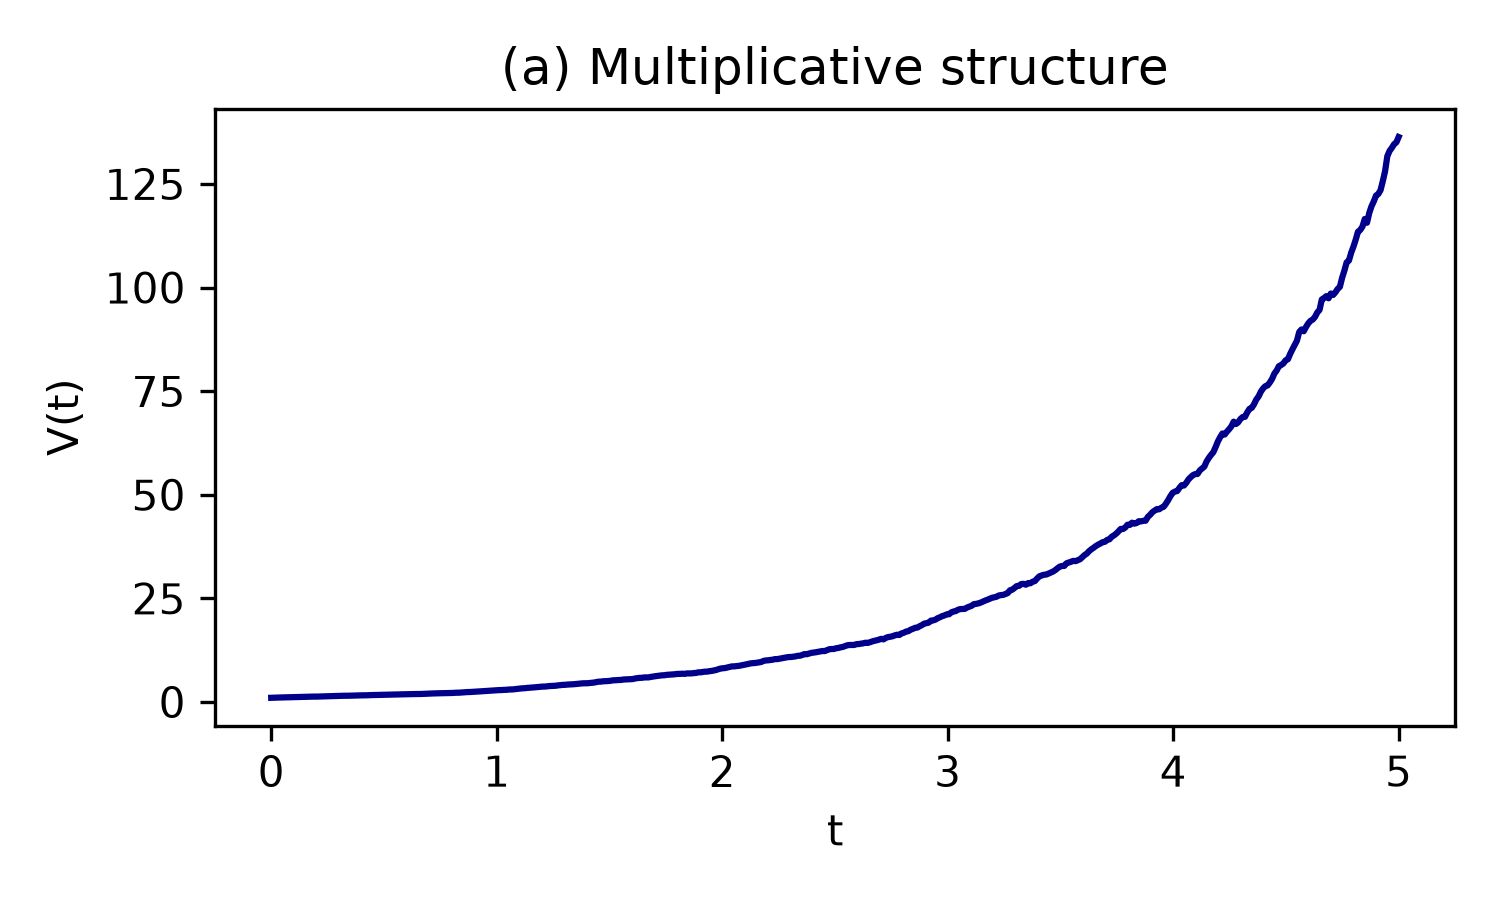
\includegraphics[width=\textwidth]{Python/figures/multiplicative_structure.png}
    \caption*{\textbf{(a) multiplicative：掛け算的悪化}\\外部ショックが企業価値に指数的に作用する構造}
\end{minipage}
\hfill
\begin{minipage}{0.33\textwidth}
    \centering
    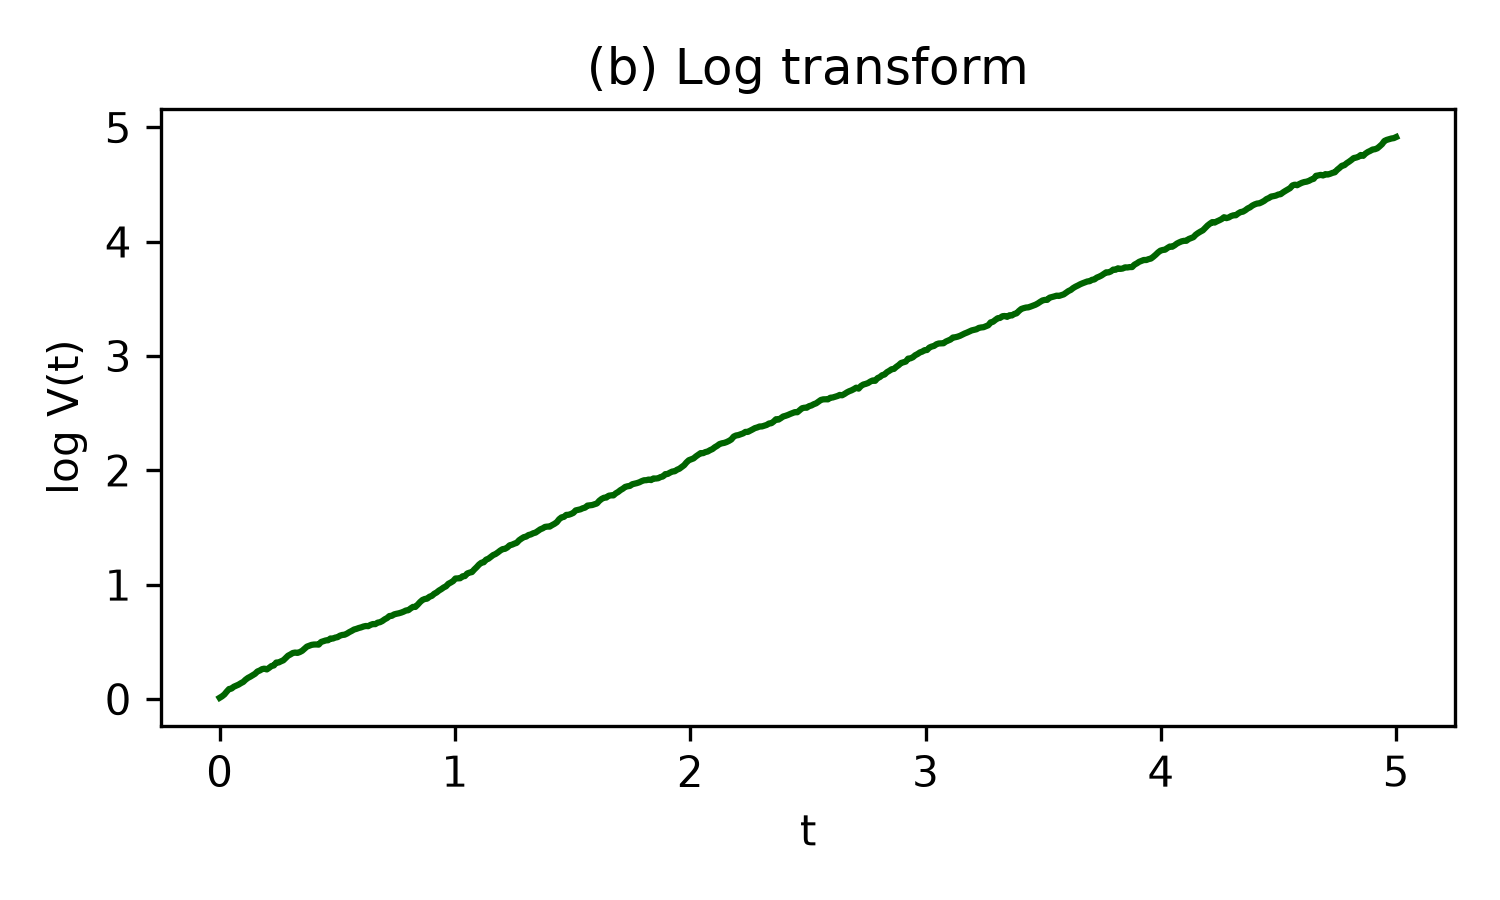
\includegraphics[width=\textwidth]{Python/figures/log_transform.png}
    \caption*{\textbf{(b) log：対数変換}\\multiplicative な変化が加法的（線形）に変換される}
\end{minipage}
\hfill
\begin{minipage}{0.33\textwidth}
    \centering
    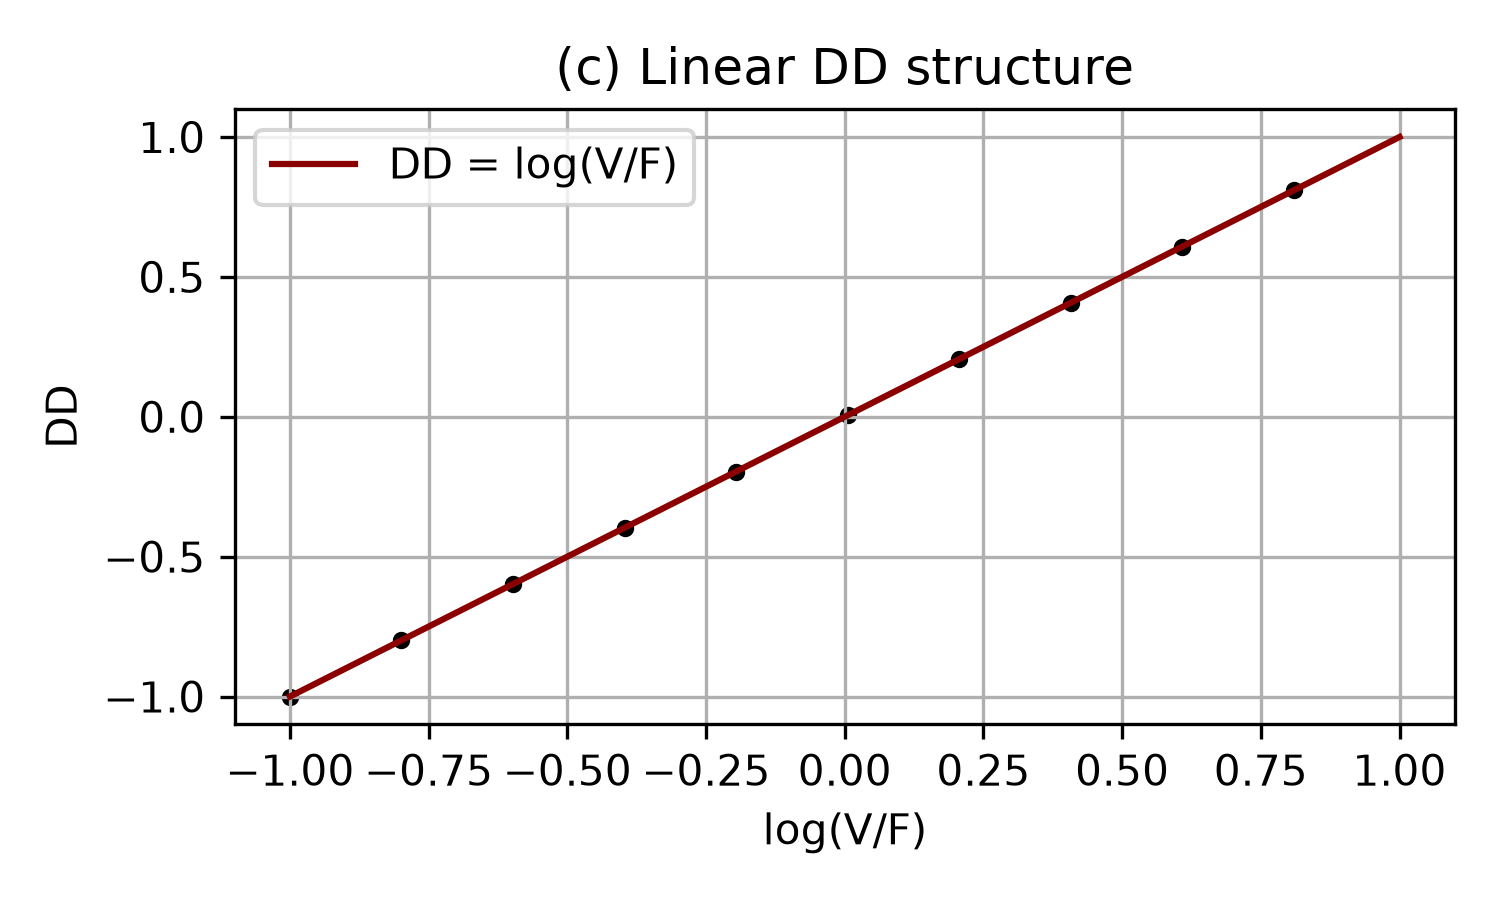
\includegraphics[width=\textwidth]{Python/figures/linear_dd.png}
    \caption*{\textbf{(c) linear：倒産距離 DD}\\閾値との差を線形距離として扱う構造}
\end{minipage}

\caption{multiplicative → log → linear の変換構造の概念図}
\label{fig:mult_log_linear}
\end{figure}

図 \ref{fig:mult_log_linear}は，企業価値の変動構造が「multiplicative（掛け算的）→ log（対数変換）→ linear（線形距離）」へと
段階的に変換される様子を概念的に示したものである。
(a) の multiplicative 構造では，外部ショックが企業価値に指数的に作用するため，
変動は時間とともに加速度的に拡大する。
(b) の log 変換では，multiplicative な変化が加法的な構造へと写像され，
企業価値の変動が線形的に扱えるようになる。
(c) の linear 構造では，倒産閾値との距離 $\log(V/F)$\footnote{
$\log(V/F)$ は Merton 型モデルにおける「倒産距離（distance to default）」の基本形であり，
企業価値 $V$ が倒産閾値 $F$（負債返済に必要な価値）からどれだけ離れているかを
対数比で測る指標である。
multiplicative（指数的）に変動する企業価値を log 変換することで，
倒産距離を加法的・線形的に扱えるようになる点が理論的な利点である。
}
が一次式として表現され，閾値との差を「線形距離」として評価できる点が
Merton 型モデルの基礎となる。

これら 3 つの図は，multiplicative な企業価値の変動が，
対数変換を経て線形な倒産距離として扱えることを視覚的に示している。


Bharath \& Shumway \parencite{BharathShumway2008} の proxy DD は，
その後の倒産研究において標準的手法として広く採用されている。
たとえば，Campbell, Hilscher \& Szilagyi \parencite{CampbellHilscherSzilagyi2008} は
市場要因と財務要因を統合した倒産モデルの中で proxy DD の有効性を示し，
Tinoco \& Wilson \parencite{TinocoWilson2013} はマクロショックと倒産距離の相互作用を実証した。
さらに Charalambakis \& Garrett \parencite{CharalambakisGarrett2019} は
産業特性を反映した倒産距離の再構築を行い，proxy DD の応用可能性を拡張している。


これらの研究は，B\&S の「機能形を維持しつつ観測可能な変数で倒産距離を構築する」
というアプローチが多様な産業・市場環境で有効であることを示している。
本研究もこの枠組みを踏まえ，新電力市場の制度的特徴に適合するよう
倒産構造を再構成する点に独自性がある。


% ---------------------------------------------
% Bharath & Shumway (2008) を採用する理論的必然性
% ---------------------------------------------

\vspace{1em}
\subsection{Bharath \& Shumway (2008) を採用する理論的必然性}

本研究が Bharath \& Shumway (2008)（以下 B\&S）を理論的基盤として採用する理由は，
新電力企業の倒産構造が Merton 型モデルの multiplicative な価値過程と整合的である一方で，
Merton モデルを直接推定することが実務的に困難であるためである。
Merton 型モデルは企業価値 $V_t$ が幾何ブラウン運動\footnote{
幾何ブラウン運動（Geometric Brownian Motion）とは、
企業価値が常に正の値をとり、ランダムに揺れながら指数的に変化する確率過程である。
本研究の視点では，この multiplicative な価値過程を前提とすることで，
企業価値の対数 $\log V_t$ が加法的（線形）な正規過程となり，
倒産閾値 $\log F$ との差 $\log(V_t/F)$ が「線形距離」として扱える点が重要となる。
この線形距離が Merton 型モデルにおける倒産距離（Distance to Default, DD）であり，
幾何ブラウン運動の仮定によって倒産確率が正規分布の累積分布として解析的に導出される。
}に従うという
multiplicative な構造を前提とし，倒産確率が次式で与えられる点に理論的な強みがある。



\[
P(\text{default}) = \Phi(-DD)
\]



この構造は，標準正規分布の図を用いることで直感的に理解できる。
図 \ref{fig:dd_normal} は，標準正規分布における倒産距離 $DD$ と
倒産確率 $\Phi(-DD)$ の関係を示している。
$DD$ が右方向に大きくなるほど，倒産確率に対応する左側の塗りつぶし部分が縮小し，
倒産確率が低下することが視覚的に理解できる。\footnote{
図では倒産確率 $\Phi(-DD)$ の定義に従い，横軸上の位置として
$-DD$ を描いている点に注意が必要である。
標準正規分布の左側の塗りつぶし部分は $\Phi(-DD)$ に対応するため，
図では「$-DD$ を左に動かすほど塗りつぶしが増える」ように見える。
しかしこれは符号の反転による見かけ上の挙動であり，
本質的には $DD$ が右方向に大きくなるほど $-DD$ は左に移動し，
結果として倒産確率 $\Phi(-DD)$ が減少する。
すなわち，図は $\Phi(-DD)$ の定義を忠実に描いているだけであり，
説明文の「$DD$ が大きいほど倒産確率が低い」という内容と
完全に整合している。
}


\begin{figure}[H]
\centering
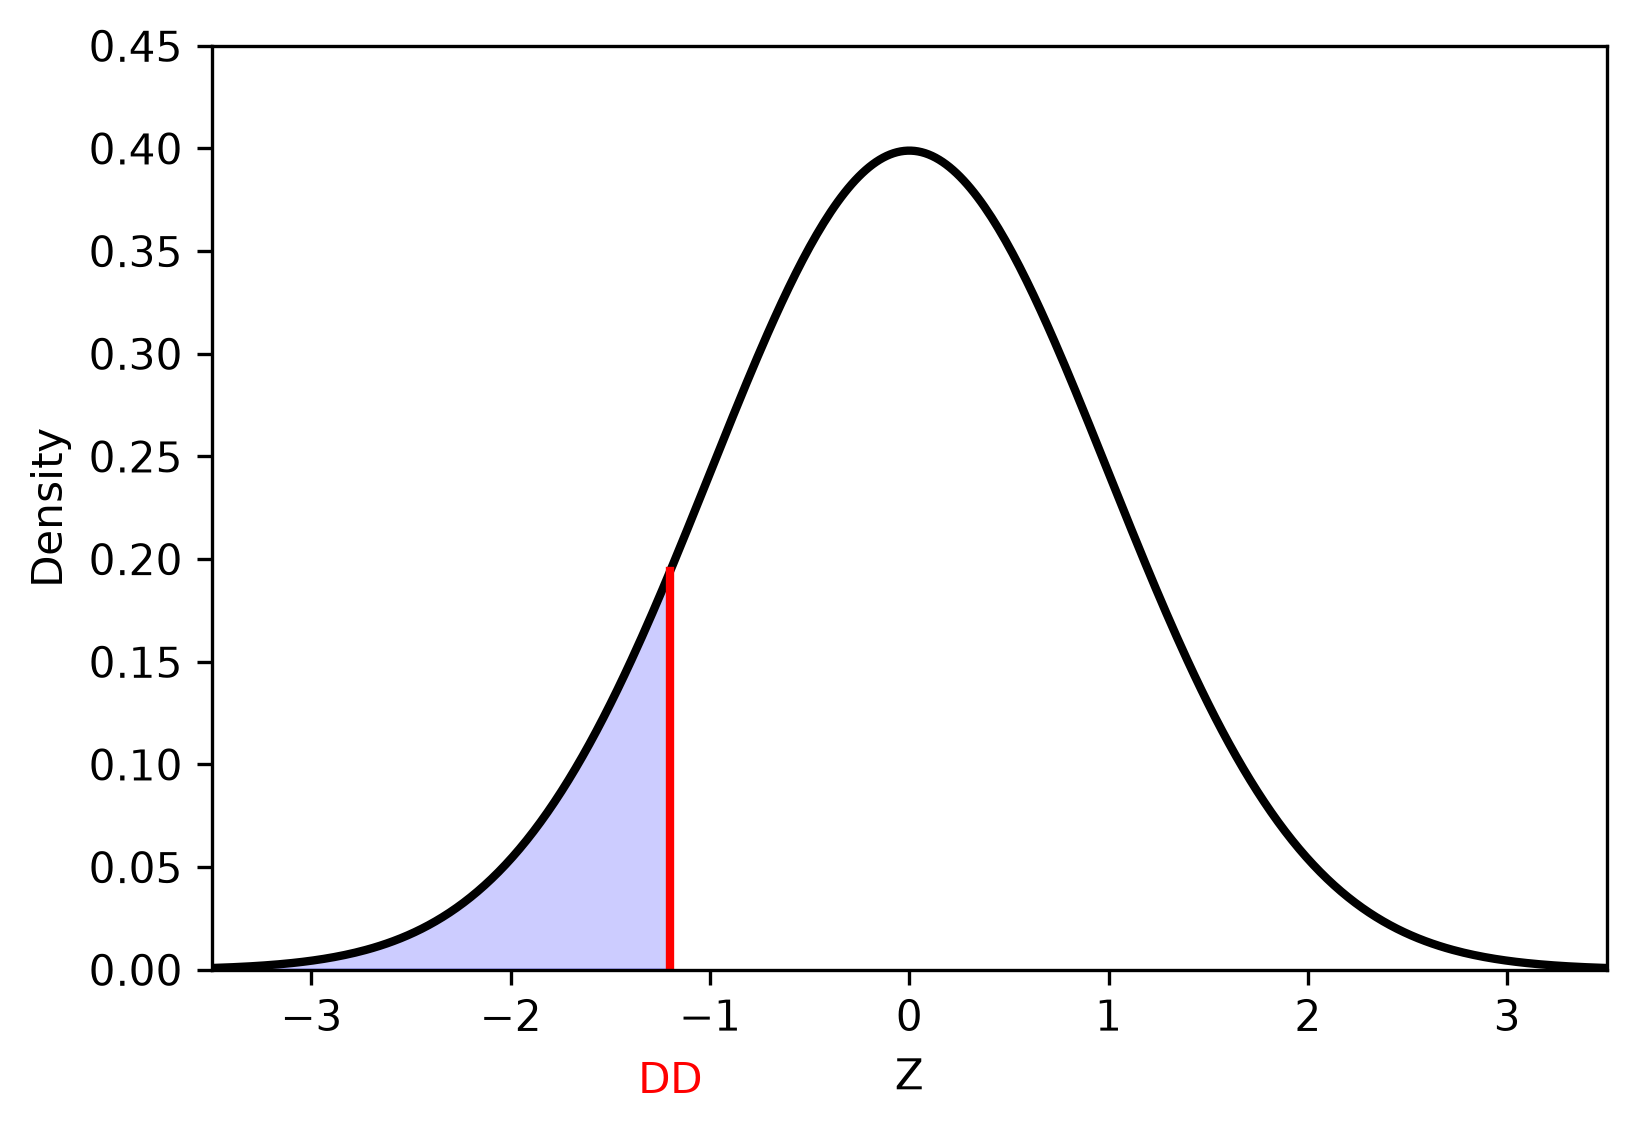
\includegraphics[width=0.85\textwidth]{figures/dd_normal.png}
\caption{標準正規分布における倒産距離 $DD$ と倒産確率 $\Phi(-DD)$}
\label{fig:dd_normal}
\end{figure}

B\&S は，この Merton 型モデルの multiplicative → log → linear の変換構造を維持しつつ，
倒産距離を観測可能な proxy によって線形化した点に独自性がある。
すなわち，Merton の理論的枠組みを損なうことなく，
倒産距離を回帰モデルで扱える形に変換した点に実務的価値がある。
この線形化の思想は，本研究が構築する四要素モデル
（収益性 $\mu$，外部ショック感応度 $\sigma$，支援能力 $S$，倒産閾値 $D$）
を実証的に検証するための理論的橋渡しとして機能する。

% ---------------------------------------------
% B&S を新電力に適用する際の前提修正の必要性
% ---------------------------------------------

\subsection{B\&S を新電力に適用する際の前提修正の必要性}

B\&S の枠組みは理論的に有効である一方で，新電力市場に適用するためには，
いくつかの前提条件を修正する必要がある。
第一に，B\&S は株価データを前提とするが，新電力企業の多くは非上場であり，
市場データを利用できない。
第二に，B\&S が想定する連続的な市場変動とは異なり，
新電力市場では JEPX 価格の急騰や制度変更など，
離散的かつ制度的ショックが倒産リスクを支配する。
第三に，B\&S の負債水準 $F$ は固定的であるのに対し，
新電力企業の倒産閾値 $D$ はインバランス料金や調達費用の変動により動的に変化する。
第四に，B\&S は親会社・自治体・金融機関による支援能力をモデルに含めていないが，
新電力企業において支援能力 $S$ は倒産リスクを大きく左右する要因である。

これらの点は B\&S の弱点ではなく，
むしろ新電力市場の制度的特殊性を反映した本研究独自の理論的貢献である\footnote{
ここで述べた前提修正は、B\&S の理論的限界を指摘するものではなく、
むしろ倒産モデルを新電力市場の制度構造に適合させるための
「構造的拡張（structural extension）」である。
すなわち、B\&S の基本枠組みを維持したまま、
市場特性に応じて倒産距離の構造要因を再定義することで、
モデルの適用範囲を拡張し、制度依存的な倒産メカニズムを
理論的に記述可能にする点に本研究の独自性がある。
この意味で、前提修正は B\&S の弱点の指摘ではなく、
新電力市場の制度的特徴を理論モデルに統合するための
学術的貢献として位置づけられる。
}
。
すなわち，本研究は B\&S の multiplicative → log → linear の構造を踏まえ，
新電力市場に特有の制度リスクを反映するために，
倒産距離の構造を四要素モデル（$\mu, \sigma, S, D$）として再構成する。
この再構成により，本研究の線形倒産距離 $Z_{\text{lin}}$ は，
B\&S の理論的系譜に属しながらも，
新電力企業の倒産メカニズムを説明するために必要な制度的要因を統合した
新たな倒産モデルとして位置づけられる。

% ---------------------------------------------
% 4.2 Merton モデル：multiplicative → log → linear の構造
% ---------------------------------------------
\section{Merton モデル：multiplicative → log → linear の構造}

本節では，Merton（1974）の構造モデルが前提とする
「multiplicative → log → linear」という価値過程の変換構造を整理し，
倒産距離（Distance to Default, DD）がどのように導出されるかを体系的に示す。
この変換構造は，企業価値の掛け算的な変動が対数変換によって線形化され，
倒産確率が標準正規分布の累積分布として表現できるという理論的特徴を持つ。

\subsection{multiplicative → log → linear の理論構造}

Merton（1974）の構造モデルは，企業価値 $V_t$ が幾何ブラウン運動に従うという
multiplicative な確率過程を前提とする点に特徴がある。企業価値のダイナミクス\footnote{
企業価値のダイナミクスとは，企業価値 $V_t$ が時間とともにどのように変化するかを記述する
確率的な運動法則を指す。Merton モデルではこの運動法則が幾何ブラウン運動として定式化され，
企業価値が掛け算的（multiplicative）に変動する構造を持つ。
この multiplicative な価値過程に対数変換を施すことで $\ln V_t$ が加法的（線形）な正規過程となり，
倒産閾値 $\ln F$ との差 $\log(V_t/F)$ が「線形距離」として扱えるようになる。
この線形距離が倒産距離（Distance to Default, DD）であり，
幾何ブラウン運動の仮定によって倒産確率が標準正規分布の累積分布
$\Phi(-DD)$ として解析的に導出される点が Merton 型モデルの理論的強みである。
}
は次式で与えられる：



\[
dV_t = \mu V_t\, dt + \sigma_V V_t\, dW_t
\]



ここで $\mu$ は企業価値の期待成長率，$\sigma_V$ は企業価値ボラティリティである。
multiplicative な価値過程に対数変換を施すと，加法的（線形）な構造へと写像される。

負債額 $F$ を倒産閾値とすると，1 年後の倒産距離（Distance to Default, DD）は



\[
DD = \frac{\ln(V/F) + (\mu - 0.5\sigma_V^2)}{\sigma_V}
\]



で表される\footnote{
この式の数学的導出（対数変換・正規分布化・閾値条件の整理）は付録Aに詳細を示している。
本文では概念構造に焦点を当てる。
}。これは倒産確率が



\[
\text{倒産確率} = f(\mu, \sigma_V, V/F)
\]



という multiplicative → log → linear の変換構造に基づいて決まることを示している。

倒産は「企業価値と負債の比率が確率的に閾値を下回るイベント」として定義され，
掛け算的なショックが対数変換を通じて線形化される点に理論的特徴がある\footnote{
倒産が「企業価値と負債の比率 $V/F$ が閾値を下回るイベント」として定義される理由は，
Merton 型モデルが企業価値 $V_t$ を基礎変数とし，負債額 $F$ を満期時点の返済義務として扱う
構造に基づく。満期時点において企業価値が負債額を下回れば倒産する。
この条件は $V_T < F$ と表され，対数変換によって $\log(V_T/F)$ が負になるかどうかという
「比率の閾値判定」に書き換えられる。さらに，$\log(V_T)$ が正規分布に従うことから，
$\log(V_T/F)$ は平均と分散をもつ線形距離として整理でき，その標準化が倒産距離
（Distance to Default, DD）となる。したがって，multiplicative → log → linear の変換構造は，
倒産イベント $V_T < F$ を「比率が閾値を下回る確率」として扱えるようにするための
数学的基盤である。
}。

\subsection{multiplicative → log → linear の変換構造が持つ大局的意味}

multiplicative → log → linear の構造は，倒産モデルにとって大局的な意味を持つ。
企業価値は外部ショックに対して掛け算的に反応するため，
multiplicative な価値過程を前提とすることは経済的にも数学的にも自然である。

さらに，multiplicative な構造は対数変換によって加法的（線形）に表現できるため，
複雑な相互作用を持つ倒産メカニズムを線形距離として扱うことが理論的に正当化される\footnote{
線形倒産距離として倒産メカニズムを扱うことは，Merton 型モデルの
multiplicative → log → linear の構造に基づき理論的に正当化されるだけでなく，
実証研究においても高い評価を得ている。Bharath \& Shumway（2008）は，
Merton の連続時間モデルを直接推定するよりも，観測可能な財務指標を用いた
線形倒産距離（proxy DD）が倒産予測の精度において優れていることを示した。
さらに Campbell, Hilscher \& Szilagyi（2008），Tinoco \& Wilson（2013），
Charalambakis \& Garrett（2019）など多くの後続研究が，
線形化された倒産距離が実務的・統計的に安定した予測性能を持つことを報告している。
このように，線形倒産距離は理論的整合性と実証的有効性の双方を備えた
倒産リスク指標として広く認められている。
}。

\subsection{Merton モデルにおける倒産距離の導出}

Merton モデルは連続時間の確率過程を前提としており，
企業価値 $V_t$ のダイナミクスを連続的に追跡し，
任意の時点 $T$ における倒産確率を理論的に導出する枠組みである。

対数変換を施すことで $\ln V_T$ が正規分布に従うことが示され，
倒産距離 $DD$ は平均と閾値の差を標準偏差で割った量として定義される：



\[
DD = \frac{\ln(V/F) + (\mu - 0.5\sigma_V^2)}{\sigma_V}
\]



倒産確率は標準正規分布の累積分布関数で表され，



\[
P(\text{default}) = \Phi(-DD)
\]



となる。倒産距離が大きいほど倒産確率は小さくなる。
倒産距離の導出過程（対数変換・正規分布化・閾値条件の整理）については，
詳細を付録Aに示している。

% ---------------------------------------------
% 4.3 Bharath \& Shumway (2008)：倒産距離の線形化と proxy 化
% ---------------------------------------------
\section{Bharath \& Shumway (2008)：倒産距離の線形化と proxy 化}

本節では，Merton モデルの理論構造（multiplicative → log → linear）を踏まえ，
その推定上の課題を解決するために Bharath \& Shumway（2008）（以下 B\&S）が提示した
離散時間モデルと proxy 化のアプローチを整理する。
Merton モデルは理論的に整合的である一方で，企業価値 $V$ や企業価値ボラティリティ
$\sigma_V$ が観測不可能であるため，連続時間モデルをそのまま推定することは
実務的に困難である。この問題意識が B\&S の出発点となった。

\subsection{連続時間モデルとしての Merton と，離散時間モデルとしての B\&S の相違}

Merton モデルは企業価値の連続的な変動を追跡し，任意時点の倒産確率を導出する
連続時間モデルである。しかし，企業価値 $V$ とそのボラティリティ $\sigma_V$ は
市場で直接観測できず，非線形方程式の同時推定が必要となるため，
実務的には不安定であることが知られている。

これに対して B\&S は，時間を離散化し，「1 年後に倒産するかどうか」という
固定された時間枠で倒産確率を推定する離散時間モデルを採用した。
すなわち，Merton の連続時間の数学的構造を捨てつつ，
multiplicative → log → linear の機能形のみを保持し，
観測可能な proxy を代入することで倒産距離を線形化した点に独自性がある。

この離散時間アプローチは，倒産が短期間に急激に顕在化する産業において
実務的にも理論的にも適合的であり，倒産予測モデルの実用性を大きく高めた。

\subsection{B\&S の naive predictor の理論的意義}

B\&S が提示した naive predictor\footnote{
Bharath \& Shumway（2008）が企業価値 $V$ や企業価値ボラティリティ $\sigma_V$ を
厳密に推定せず，観測可能な株式価値や負債額をそのまま代入して構築した
「素朴な（naive）倒産距離」を指す。
} は次式で与えられる：



\[
DD_{\text{naive}}
= \frac{\ln\left(\frac{E+F}{F}\right) + (\hat{\mu}-0.5\hat{\sigma}_V^2)}{\hat{\sigma}_V}
\]



ここで，
\begin{itemize}
    \item $\hat{\mu}$：株価リターン等から推定される収益性の proxy  
    \item $\hat{\sigma}_V$：株価ボラティリティから推定される企業価値ボラティリティの proxy  
\end{itemize}

この式は，Merton モデルの multiplicative → log → linear の構造を保持しつつ，
観測可能な proxy を代入することで推定可能性を確保したものである。
B\&S の重要な結論は「企業価値 $V$ と $\sigma_V$ の同時推定は必須ではない」という点にあり，
線形化された倒産距離が実務的に十分であることを示した。

\subsection{proxy 化の実務的意義と限界}

B\&S の proxy 化は倒産予測の実務に大きなインパクトを与えた\footnote{
Campbell, Hilscher \& Szilagyi（2008），Tinoco \& Wilson（2013），
Charalambakis \& Garrett（2019）など多くの後続研究が，
proxy DD が従来の財務指標よりも倒産予測精度に優れることを示している。
}。
株価データを用いることで，従来困難だった倒産距離の推定が可能となり，
信用リスク管理や企業モニタリングに広く応用された。

しかし，このアプローチには限界もある。

第一に，株価データを前提とするため非上場企業には適用困難である。  
第二に，市場ショックの連続性を前提とするが，新電力市場では離散的ショックが支配的である。  
第三に，負債水準を固定的に扱うが，新電力企業ではインバランス料金や調達費用により動的に変化する。  
第四に，支援能力をモデルに含めていないため，新電力企業特有の親会社・自治体・金融機関による
支援効果を捉えられない。

\subsection{B\&S の限界と，本研究における再構成の必要性}

以上の限界を踏まえ，本研究は B\&S の「proxy による線形化」という枠組みを土台とし，
新電力市場の制度的特徴を反映した四要素モデル
（収益性 $\mu$，外部ショック感応度 $\sigma$，支援能力 $S$，倒産閾値 $D$）
を構築し，線形倒産距離 $Z_{\text{lin}}$ として再定式化する。



\[
Z_{\text{lin}} = a\mu - b\sigma + cS - dD
\]



この $Z_{\text{lin}}$ は，Merton モデルの倒産距離および B\&S の proxy DD の機能形を継承しつつ，
新電力市場の制度的特徴を統合した新たな倒産モデルとして位置づけられる。

% ---------------------------------------------
% 4.4 本研究の線形倒産距離 $Z_{\text{lin}}$：新電力企業への写像
% ---------------------------------------------

\section{本研究の線形倒産距離 $Z_{\text{lin}}$：新電力企業への写像}

本節では，新電力企業の倒産メカニズムを構造的に整理し，
その主要因を観測可能な四要素（収益性 $\mu$，外部ショック感応度 $\sigma$，
支援能力 $S$，倒産閾値 $D$）として再構成したうえで，
これらを線形倒産距離 $Z_{\text{lin}}$ として形式化する。

新電力企業の倒産は，複数の要因が短期間に同時悪化することで急激に顕在化する。
既存の倒産事例（F-Power，エルピオ，ハルエネ等）では，
(i) 収益性の低下，(ii) 外部ショックへの脆弱性，
(iii) 支援能力の不足，(iv) 外部ショック時の支払義務の急増，
という四つの要因が繰り返し確認されており，
これらが倒産発生の主要因を網羅する「必要かつ十分な最小構成」であることが示されている。

この四要素はすべて観測可能な財務指標として定量化でき，
新電力企業の倒産メカニズムを構造的に捉えるうえで互いに独立である。
したがって，本研究はこれら四要素を倒産距離の構成要因として採用する。



\[
Z_{\text{lin}} = a\mu - b\sigma + cS - dD
\]



ここで，
\begin{itemize}
    \item $\mu$：収益性（営業利益率等）
    \item $\sigma$：外部ショック感応度（スポット依存度等）
    \item $S$：支援能力（親会社・自治体・金融機関）
    \item $D$：倒産閾値（外部ショック時の支払義務）
\end{itemize}

この $Z_{\text{lin}}$ は，数学的には四要素の線形結合であるが，
その背後には Merton モデルが前提とする
multiplicative → log → linear の構造が存在している。
すなわち，掛け算的に悪化する倒産要因を対数変換によって線形距離として扱うという
Merton 型モデルの機能形を保持しつつ，
観測可能な財務指標によって倒産距離を近似するという
Bharath \& Shumway（2008）の proxy 化の思想を継承している。

本研究の $Z_{\text{lin}}$ は，Merton → B\&S の理論的系譜に属しながら，
新電力市場の制度的特徴（支援能力の存在，動的な倒産閾値，離散的ショック）を統合した
新たな倒産距離として位置づけられる。

\begin{table}[H]
\centering
\caption{Merton → B\&S → 本研究の $Z_{\text{lin}}$ の対応関係}
\label{tab:merton_bs_zlin}

\renewcommand{\arraystretch}{1.4}
\begin{tabularx}{\textwidth}{p{0.22\textwidth} p{0.28\textwidth} X}
\toprule
\textbf{Merton (1974)} & \textbf{B\&S (2008)} & \textbf{本研究の $Z_{\text{lin}}$} \\
\midrule

$\mu$（企業価値の期待成長率） &
過去リターン等で proxy &
収益性（営業利益率） \\

$\sigma_V$（企業価値ボラティリティ） &
株価ボラティリティで proxy &
外部ショック感応度（スポット依存度） \\

$F$（負債額） &
帳簿価値で proxy &
倒産閾値 $D$（外部ショック時の支払義務） \\

--- & --- &
支援能力 $S$（外生的緩和要因） \\

\midrule

倒産距離 $DD$ &
naive DD（proxy DD） &
$Z_{\text{lin}}$（線形倒産距離） \\

\bottomrule
\end{tabularx}
\end{table}

以上より，$Z_{\text{lin}}$ は

\begin{quote}
Merton モデルの倒産距離を B\&S の proxy 化の思想に基づき線形化し，
新電力企業の制度的特徴を反映するよう再構築した潜在倒産距離
\end{quote}

として理論的に位置づけられる。

次章では，この $Z_{\text{lin}}$ を Ordered Logit モデルに接続し，
新電力企業の倒産ステージ（Active → Administration → Liquidation → Dissolved）へと
離散的に写像することで，実証分析を行う。

% ---------------------------------------------
% 4.5 連続的倒産距離 $Z_{\text{lin}}$ と Ordered Logit の接続
% ---------------------------------------------

\section{連続的倒産距離 $Z_{\text{lin}}$ と Ordered Logit の接続}

前節で導出した線形倒産距離 $Z_{\text{lin}}$\footnote{
潜在変数（latent index）を $Z$ と表記するのは計量経済学の慣例であり，
特別な理論的意味を持つわけではない。
} は，新電力企業の倒産リスクを連続的な尺度として表す潜在倒産距離である。
しかし，実際の倒産データは連続量として観測されるわけではなく，
企業はある時点で「存続」「財務悪化」「撤退・吸収合併」「法的倒産」といった
離散的なステージに分類される。

したがって，連続的倒産距離 $Z_{\text{lin}}$ を実証分析で扱うためには，
連続量を離散カテゴリへ写像する確率構造が必要となる。
この橋渡しを行う標準的な枠組みが Ordered Logit モデルである。

\subsection{Ordered Logit モデルの潜在変数構造}

Ordered Logit モデルは，倒産の背後に連続的な潜在変数 $y^*_{i,t}$ が存在すると仮定し，
その値が複数の閾値（cutpoints）$\tau_1, \tau_2, \tau_3$ をどこまで超えるかによって，
離散的な倒産ステージが決定されるという構造を持つ。

潜在変数は次式で表される：

\begin{equation}
y^*_{i,t}
=
\beta_1 D_{i,t}
+ \beta_2 \mu_{i,t}
+ \beta_3 \sigma_{i,t}
+ \beta_4 S_{i,t}
+ \varepsilon_{i,t},
\qquad
\varepsilon_{i,t} \sim \text{Logistic}(0,1)
\label{eq:latent_y_appendix}
\end{equation}

式 \eqref{eq:latent_y_appendix} の線形部分 $X_{i,t}\beta$ は，
第4章で導出した線形倒産距離



\[
Z_{\text{lin}} = a\mu - b\sigma + cS - dD
\]



と構造的に一致している。
すなわち，$Z_{\text{lin}}$ を Ordered Logit の潜在変数 $y^*$ に写像することで，
理論モデル（連続的倒産距離）と実証モデル（離散的倒産ステージ）が
自然に接続される。

\subsection{cutpoint（閾値）の推定と離散カテゴリへの写像}

Ordered Logit モデルにおける cutpoint（閾値）$\tau_k$ は，
研究者が任意に設定する境界ではなく，
ロジット係数 $\beta$ と同様に尤度最大化（MLE）によって
データから推定される内生的パラメータである。
この性質により，潜在変数の連続スケールをどのように区切るべきかを
モデル自身がデータから学習することが可能となり，
倒産ステージの境界を恣意的に設定する必要がない。

\subsection{本研究における Ordered Logit の役割}

以上より，Ordered Logit モデルは，
第4章で導出した連続的倒産距離 $Z_{\text{lin}}$ を，
実証分析で扱う離散的倒産ステージへと変換するための
数学的に整合的な枠組みである。

次章では，この Ordered Logit モデルを用いて，
日本企業および英国企業の倒産ステージを推定し，
四要素モデル（$\mu, \sigma, S, D$）が倒産リスクをどのように規定するかを
実証的に検証する。

% ---------------------------------------------
% 4.6 Bharath \& Shumway (2008) と本研究の比較
% ---------------------------------------------

\section{Bharath \& Shumway (2008) と本研究の比較}
\label{sec:bs_comparison}

本節では，Bharath \& Shumway（2008）（以下 B\&S）が提示した
proxy 化による倒産距離と，本研究が構築した線形倒産距離
$Z_{\text{lin}}$ の関係を整理し，両者の共通点と相違点を明確化する。

B\&S は，Merton モデルの連続時間構造を直接推定するのではなく，
multiplicative → log → linear の機能形を保持したまま，
観測可能な財務指標を代入することで倒産距離を線形化した。
この「機能形を維持しつつ観測可能な変数で倒産距離を構築する」という
アプローチは，その後の倒産研究において標準的手法として広く採用されている。
たとえば Campbell, Hilscher \& Szilagyi (2008) は市場要因と財務要因を統合した
倒産モデルの中で proxy DD の有効性を示し，
Tinoco \& Wilson (2013) はマクロショックと倒産距離の相互作用を実証した。
さらに Charalambakis \& Garrett (2019) は産業特性を反映した倒産距離の再構築を行い，
proxy DD の応用可能性を拡張している。

本研究はこの B\&S の枠組みを継承しつつ，
新電力市場の制度的特徴（離散的ショック，動的な倒産閾値，支援能力の存在）を
反映するために倒産距離を再構成した。
すなわち，収益性 $\mu$，外部ショック感応度 $\sigma$，
支援能力 $S$，倒産閾値 $D$ の四要素を観測可能変数として導入し，
新電力企業の倒産メカニズムに適合する線形倒産距離
$Z_{\text{lin}}$ を構築した点に独自性がある。

以下では，B\&S と本研究の線形倒産距離の対応関係を整理する。

\begin{table}[H]
\centering
\caption{Bharath \& Shumway (2008) と本研究の比較}
\label{tab:bs_vs_this}

\renewcommand{\arraystretch}{1.4}
\begin{tabularx}{\textwidth}{p{0.28\textwidth} p{0.30\textwidth} X}
\toprule
\textbf{項目} & \textbf{Bharath \& Shumway (2008)} & \textbf{本研究（新電力倒産モデル）} \\
\midrule

理論的基盤 &
Merton 型モデルの倒産距離を proxy 化 &
Merton/B\&S の構造を新電力の制度構造に写像し再構成 \\

倒産距離の構造 &
$\mu$, $\sigma_V$, $V/F$ に基づく線形倒産距離 &
収益性 $\mu$, 外部ショック感応度 $\sigma$, 支援能力 $S$, 倒産閾値 $D$ に基づく線形倒産距離 $Z_{\text{lin}}$ \\

扱うリスク要因 &
市場リスク・財務リスク（株価データ中心） &
外部ショック（JEPX 価格・制度コスト），支援能力，倒産閾値の変動など新電力特有の制度的リスク \\

目的 &
企業価値モデルの proxy 化と倒産予測精度の向上 &
新電力市場に特有の倒産構造の理論的解明と倒産距離の再構築 \\

独自性 &
Merton の機能形を維持した proxy DD の提案 &
四要素モデル（$\mu, \sigma, S, D$）を用いた新電力特有の倒産距離の構築 \\

\bottomrule
\end{tabularx}
\end{table}

以上より，本研究の $Z_{\text{lin}}$ は，
B\&S の理論的系譜に属しながらも，
新電力企業の倒産メカニズムを説明するために必要な制度的要因を統合した
新たな倒産距離として位置づけられる。

% ============================================================
% 第5章 Ordered Logit モデル：倒産距離 Z_lin の離散化と推定
% ============================================================

\chapter{Ordered Logit モデル：倒産距離 $Z_{\text{lin}}$ の離散化と推定}
\label{chap:ordered_logit}

\graphicspath{{figures/}}

本章では，第4章で導出した連続的倒産距離 $Z_{\text{lin}}$ を，
実証分析で扱う離散的な倒産ステージへと接続するための統計モデルとして，
Ordered Logit モデルを導入する。

倒産距離 $Z_{\text{lin}}$ は，企業価値プロセスと倒産閾値の関係を
連続的な尺度として表す理論モデルであるが，
実際の倒産データは「存続」「財務悪化」「撤退・吸収合併」「法的倒産」といった
離散的なステージとして観測される。
したがって，理論モデルで得られた連続量を，
実証分析で扱う離散カテゴリへと整合的に写像する枠組みが必要となる。

本章は，この写像を数学的に実現する Ordered Logit モデルの理論構造を提示し，
倒産距離 $Z_{\text{lin}}$ と潜在変数モデル $y^*$ の対応関係を明確化する章である。
まず，理論モデル・統計モデル・確率モデルがどのように連続的に接続されるかを
三層構造として整理し，Ordered Logit の導入位置づけを明確にする。


% ============================================================
% 5.1 理論モデル・統計モデル・確率モデルの三層構造
% ============================================================

\section{理論モデル・統計モデル・確率モデルの三層構造}
\label{sec:three_layer_structure}

本節では，本研究の倒産分析がどのように
「理論モデル（構造モデル）→ 統計モデル（潜在変数モデル）→ 確率モデル（Ordered Logit）」
という三層構造で接続されているかを整理する。

第4章で導出した線形倒産距離 $Z_{\text{lin}}$ は，
倒産距離 DD の一次近似\footnote{
ここでいう「一次近似」とは，Merton 型倒産距離の構造
（平均 $-$ 閾値）／不確実性を代表点の近傍で線形化したものであり，
Bharath \& Shumway（2008）の proxy DD の式そのものを展開したものではない。
}として倒産リスクの構造を表す決定論的指標である。
この連続的倒産距離を，観測可能データを用いて推定するためには，
潜在変数モデル $y^* = X\beta + \varepsilon$ に写像する必要がある。

さらに，潜在変数が複数の閾値 $\tau_k$ を跨ぐ構造を確率モデルへ接続することで，
Ordered Logit による離散的倒産ステージの確率的生成が実現される。

表 \ref{tab:theory_empirical_mapping} は，この対応関係を三つのステップとしてまとめたものである。

\begin{table}[H]
\centering
\caption{理論モデルと実証モデルの構造的対応（3ステップ）}
\label{tab:theory_empirical_mapping}
\begin{tabular}{p{3cm} p{6cm} p{6cm}}
\toprule
ステップ & 数式 & 役割 \\
\midrule
(1) 理論モデル（構造モデル） &
\(\displaystyle Z_{\text{lin}} = a\mu - b\sigma + cS - dThr\) &
倒産距離 DD の構造を一次近似した決定論的モデル \\

(2) 統計モデル（潜在変数モデル） &
\(\displaystyle y^* = X\beta + \varepsilon\) &
構造モデルを観測可能変数で推定するための統計的枠組み \\

(3) 確率モデル（Ordered Logit） &
\(\displaystyle \Pr(y=k)=\Lambda(\tau_k - X\beta)-\Lambda(\tau_{k-1}-X\beta)\) &
潜在変数を閾値で区切り，倒産ステージ確率を生成する \\
\bottomrule
\end{tabular}
\end{table}

図 \ref{fig:structural_mapping} に，理論モデル（\(Z_{\text{lin}}\)）と Ordered Logit の潜在変数モデルの構造的対応を示す。

\begin{figure}[H]
\centering
\begin{tikzpicture}[node distance=2.5cm]

\node[rectangle, draw, rounded corners, text width=7cm, align=center] (theory)
{\textbf{理論モデル（構造モデル）}\par
\(\displaystyle Z_{\text{lin}} = a\mu - b\sigma + cS - dThr\)
};

\node[rectangle, draw, rounded corners, text width=7cm, align=center, below=of theory] (latent)
{\textbf{統計モデル（潜在変数モデル）}\par
\(\displaystyle y^*_{i,t} = X_{i,t}\beta + \varepsilon_{i,t}\)\par
\(\displaystyle \varepsilon_{i,t} \sim \text{Logistic}(0,1)\)
};

\node[rectangle, draw, rounded corners, text width=8cm, align=center, below=of latent] (ordered)
{\textbf{確率モデル（Ordered Logit）}\par
閾値 \(\tau_k\) に基づくステージ確率\par
\(\displaystyle \Pr(y=k)=\Lambda(\tau_k - X\beta)-\Lambda(\tau_{k-1}-X\beta)\)
};

\draw[->, thick] (theory) -- node[midway, right]{構造的対応（写像）} (latent);
\draw[->, thick] (latent) -- node[midway, right]{ロジスティック分布により確率化} (ordered);

\end{tikzpicture}

\caption{理論モデル（\(Z_{\text{lin}}\)）と Ordered Logit の潜在変数モデルの構造的対応}
\label{fig:structural_mapping}
\end{figure}

% ============================================================
% 5.2 Ordered Logit の潜在変数構造
% ============================================================

\section{Ordered Logit の潜在変数構造}
\label{sec:ordered_latent_structure}

Ordered Logit モデルは，倒産ステージの背後に連続的な潜在変数
$y^*_{i,t}$ が存在すると仮定する潜在変数モデルである。
潜在変数は，企業の財務状態や市場環境など，倒産リスクに影響する要因を
線形に統合した上で，観測できないショックを加えたものである。

潜在変数モデルは次式で表される。


\[
y^*_{i,t}
=
X_{i,t}\beta + \varepsilon_{i,t},
\qquad
\varepsilon_{i,t} \sim \text{Logistic}(0,1)
\]



ここで，

\begin{itemize}
    \item $X_{i,t}$：倒産リスクに影響する観測可能な説明変数ベクトル  
    \item $\beta$：各説明変数の影響度を表す係数  
    \item $\varepsilon_{i,t}$：観測できないショック（ロジスティック分布に従う）
\end{itemize}

である。

ロジスティック分布を仮定することで，潜在変数が閾値を超える確率が
ロジスティック関数（ロジット確率）として表される。
この確率構造が Ordered Logit の基礎となる。

潜在変数の期待値は次式で与えられる。



\[
E[y^*_{i,t}] = X_{i,t}\beta
\]



これは，潜在倒産リスクの「中心」を表す量であり，
後述する線形倒産距離 $Z_{\text{lin}}$ と構造的に対応する。

潜在変数 $y^*$ は観測されないが，
その値が複数の閾値（cutpoints）をどこまで超えるかによって，
観測される倒産ステージが決定される。
この閾値構造については次節で詳述する。

% ============================================================
% 5.3 Ordered Logit の閾値構造（cutpoints）
% ============================================================

\section{Ordered Logit の閾値構造（cutpoints）}
\label{sec:ordered_cutpoints}

第3章では，倒産を「潜在変数が複数の閾値を跨ぐ現象」として捉える
Ordered Logit（順序ロジット）モデルの理論構造を示し，
倒産距離 DD の一次近似と閾値の役割がどのように接続されるかを整理した。
本節では，その理論的枠組みを踏まえつつ，
倒産が複数の段階と異なる「重さ（severity）」\footnote{
ここでいう「重さ（severity）」とは，倒産を単なる発生有無ではなく，
どの程度深刻な状態に至ったかという段階的な違いを表す概念である。
倒産研究では，破産・民事再生・撤退・吸収合併などの退出イベントは
企業にとって異なる経済的影響を持つため，
これらを区別せず二値化すると情報が大きく失われることが指摘されている
（Altman and Hotchkiss, 2006；Campbell, Hilscher and Szilagyi, 2008）。
Ordered Logit モデルは，こうした倒産の深刻度（severity）を
複数の段階として扱うことで，倒産プロセスの異質性をより精緻に捉えることができる。
}
を伴う現象であることを踏まえ，
従来の二値ロジットモデルでは新電力企業の倒産データを適切に扱えない理由を明確化し，
Ordered Logit を採用する必然性を示す。


\subsection*{二値ロジットの構造的限界：完全分離の問題}

新電力企業の倒産は極めて稀であり，
倒産＝1 の観測値が全体のごく一部に限られる。
このようなデータ構造では，従来の二値ロジットモデルにおいて
\textbf{完全分離（perfect separation）} が発生しやすい。
完全分離とは，説明変数の組み合わせが倒産企業と非倒産企業を
完全に識別してしまう状況を指す。
具体的には，ある説明変数の領域に倒産企業しか存在しない，
または非倒産企業しか存在しないという「完全な区分」が生じると，
ロジットモデルの尤度最大化において係数が無限大方向へ発散し，
有限の最尤推定量が存在しなくなる\footnote{
完全分離（perfect separation）とは，説明変数の組み合わせが
倒産＝1 と非倒産＝0 の観測値を完全に識別してしまう状況を指す。
具体的には，ある説明変数の領域に倒産企業しか存在しない，
または非倒産企業しか存在しないという「完全な区分」が生じると，
ロジットモデルの尤度最大化において係数が無限大方向へ発散し，
有限の最尤推定量が存在しなくなる。
ロジットモデルは


\[
\Pr(\text{Default}=1)=\Lambda(X\beta)
\]


という確率構造を持つため，倒産と非倒産が完全に分離されると，
$\Lambda(X\beta)$ を 0 または 1 に近づけるために
$X\beta$ を無限大にする必要が生じ，推定が数学的に不可能となる。
倒産企業が極端に少ない産業では典型的に発生する問題であり，
本研究の新電力企業データでも同様の現象が確認された。
}。

本研究でも，当初は倒産を二値（0/1）で定義したロジット推計を試みたが，
倒産企業が極めて少ないため，説明変数の組み合わせが
倒産と非倒産を完全に識別してしまい，最尤推定が発散する現象が確認された。
このため，倒産を二値で扱う枠組みでは，
新電力企業の倒産リスクを安定的に推定することができない。

\subsection*{倒産の段階性と Ordered Logit の必要性}

新電力企業の倒産プロセスは，単なる「倒産／非倒産」という二値ではなく，
財務悪化，撤退・吸収合併，法的倒産といった
\textbf{複数の段階を持つ現象}として観測される。
この段階性をモデル化するためには，
潜在変数 $y^*_{i,t}$ が複数の閾値（cutpoints）をどこまで超えるかによって
観測される倒産ステージが決定されるという構造が必要となる。

Ordered Logit モデルは，この「連続量 → 離散カテゴリ」の写像を
数学的に整合的に実現する標準的な枠組みである。
潜在変数 $y^*_{i,t}$ と倒産ステージの関係は次式で表される。



\[
\text{default\_stage}_{i,t} =
\begin{cases}
0 & (y^*_{i,t} < \tau_1) \\
1 & (\tau_1 \le y^*_{i,t} < \tau_2) \\
2 & (\tau_2 \le y^*_{i,t} < \tau_3) \\
3 & (\tau_3 \le y^*_{i,t})
\end{cases}
\]



ここで，

\begin{itemize}
    \item $\tau_1$：存続ステージと財務悪化ステージを分ける閾値  
    \item $\tau_2$：財務悪化ステージと撤退・吸収合併ステージを分ける閾値  
    \item $\tau_3$：撤退・吸収合併ステージと法的倒産ステージを分ける閾値  
\end{itemize}

である。

重要なのは，cutpoint（閾値）$\tau_k$ が研究者によって外生的に設定される値ではなく，
ロジット係数 $\beta$ と同様に尤度最大化（MLE）によって
\textbf{データから推定される内生的パラメータ}である点である。
つまり，閾値は「理論的に固定された境界」ではなく，
観測データとロジスティック分布の整合性を最も高めるように
推定される境界点である。

このため，潜在変数が特定の区間（例：$\tau_1 \le y^* < \tau_2$）に位置する場合でも，
Ordered Logit は 4 つのステージすべての確率を同時に計算する。
しかし，観測される倒産ステージは「最も確率が高いステージ」ではなく，
潜在変数がどの閾値区間に位置するかによって機械的に分類される。

\subsection*{本研究における実証的実装}

本研究では，観測可能性の制約から，
理論編で導入した 4 段階モデルを 3 段階モデルへ簡略化して推定する。
第4章で整形した財務データ・市場データを基礎として，
Ordered Logit 推定に必要な説明変数（debt\_ratio, asset\_growth, sigma）と
倒産ステージ（0・1・2）を付与し，
推定用パネルデータとして再構築した。

以上の理由から，Ordered Logit モデルは，
新電力企業の倒産リスクを複数段階の現象として扱うための
理論的・実証的に最も整合的な枠組みである。

% ============================================================
% 5.4 線形倒産距離 $Z_{\text{lin}}$ と潜在変数 $y^*$ の構造的対応
% ============================================================

\section{線形倒産距離 $Z_{\text{lin}}$ と潜在変数 $y^*$ の構造的対応}
\label{sec:zlin_y_mapping}

Bharath \& Shumway（2008）の倒産距離（proxy DD）は，
Merton 型モデルの「multiplicative → log → linear」という構造を保持したまま，
観測可能な財務データへ写像したものである。

本節では，第4章で導出した線形倒産距離 $Z_{\text{lin}}$ と，
Ordered Logit モデルの潜在変数 $y^*_{i,t}$ がどのように構造的に対応しているかを整理する。
この対応関係を明確にすることで，理論モデル（構造モデル）と統計モデル（潜在変数モデル）が
どのように連続的に接続されるかが理解できる。

% ------------------------------------------------------------
% (1) 記号と経済的意味の整理
% ------------------------------------------------------------

\subsection*{(1) 記号と経済的意味の整理}

まず，本研究で用いる主要な記号とその経済的意味を整理する。

\begin{table}[H]
\centering
\caption{潜在変数／倒産距離／閾値の記号整理}
\label{tab:latent_vars_unified}
\resizebox{\textwidth}{!}{%
\begin{tabular}{lll}
\hline
記号・呼称 & 数式上の定義 & 経済的意味 \\
\hline
$y^*$ & $X\beta$ & 潜在倒産リスク（連続値） \\
$Z_{\text{lin}}$ & $X\beta$ & 線形倒産距離（倒産閾値からの距離） \\
線形予測子 &
$X\beta = \beta_1 D + \beta_2 \mu + \beta_3 \sigma + \beta_4 S + \cdots$
& 倒産リスクに影響する要因の総合効果 \\
$\tau_k$ & cutpoints & 倒産ステージを区切る閾値 \\
$y$ & 0--3 & 観測される倒産ステージ \\
\hline
\end{tabular}
}
\end{table}

表~\ref{tab:latent_vars_unified} に示すように，
$X\beta$ は統計モデルと理論モデルの双方で現れるが，
その意味と役割は三者で明確に異なる。

\begin{itemize}
    \item \textbf{線形予測子 $X\beta$（統計モデル）}：  
    潜在変数の期待値（中心）を表す統計的概念。
    \item \textbf{潜在変数 $y^*$（確率モデル）}：  
    $X\beta$ に誤差項を加えた確率モデルの内部構造。
    \item \textbf{線形倒産距離 $Z_{\text{lin}}$（理論モデル）}：  
    倒産距離 DD を一次近似した決定論的指標。
\end{itemize}

数式の形は一致していても，意味は異なる点に注意が必要である。

% ------------------------------------------------------------
% (2) Zlin と y* の構造的対応
% ------------------------------------------------------------

\subsection*{(2) $Z_{\text{lin}}$ と $y^*$ の構造的対応}

Ordered Logit の潜在変数モデルは次式で表される。


\[
y^*_{i,t}
=
X_{i,t}\beta + \varepsilon_{i,t},
\qquad
\varepsilon_{i,t} \sim \text{Logistic}(0,1)
\]



ここで $X\beta$ は潜在倒産リスクの中心（期待値）を表す。

一方，第4章で導出した線形倒産距離は，


\[
Z_{\text{lin}} = a\mu - b\sigma + cS - dD
\]



であり，これは Ordered Logit の線形部分 $X\beta$ と同じ構造を持つ。

したがって，



\[
X\beta \;\;\longleftrightarrow\;\; Z_{\text{lin}}
\]



という対応関係が成立する。

さらに，潜在変数は



\[
y^*_{i,t} = Z_{\text{lin}} + \varepsilon_{i,t}
\]



と解釈でき，理論モデルで導出した倒産距離に観測できないショックを加えたものが
Ordered Logit の潜在変数である。

% ------------------------------------------------------------
% (3) 潜在変数の散らばりとロジスティック曲線
% ------------------------------------------------------------

\subsection*{(3) 潜在変数の散らばりとロジスティック曲線}

潜在変数 $y^*$ は誤差項によって上下に揺らぐ。
図~\ref{fig:latent_error_logistic} は，潜在変数の散らばりとロジスティック曲線の関係を示す。

\begin{figure}[H]
    \centering
    \begin{tikzpicture}
        \begin{axis}[
            width=0.9\linewidth,
            height=7cm,
            xmin=-4, xmax=4,
            ymin=-2, ymax=2,
            axis lines=middle,
            xlabel={潜在変数の理論値 $X\beta$},
            ylabel={潜在変数 $y^*$},
            samples=200
        ]
        \addplot[black, thick] {0.5*x};
        \addplot[
            only marks,
            mark=*,
            mark size=1.8pt,
            blue!60
        ]
        table {
            x   y
            -3.5 -2.0
            -2.5 -0.8
            -1.5 -0.3
            -0.5 -0.6
             0.5  0.7
             1.5 -0.9
             2.5  1.4
             3.5 -1.2
        };
        \addplot[
            red,
            thick,
            domain=-4:4
        ] {1/(1 + exp(-x))};
        \node at (axis cs:-3.5,0.8) [anchor=west, red] {ロジスティック曲線（確率）};
        \node at (axis cs:-3.5,-1.5) [anchor=west, blue!70] {潜在変数の散らばり（誤差項）};
        \node at (axis cs:2.2,1.2) [anchor=west, black] {$X\beta$（理論値）};
        \end{axis}
    \end{tikzpicture}
    \caption{潜在変数の散らばり（誤差項）とロジスティック曲線の関係}
    \label{fig:latent_error_logistic}
\end{figure}

青点は潜在変数のゆらぎを示す説明図であり，
赤線は倒産確率を表すロジスティック曲線である。

% ------------------------------------------------------------
% (4) 理論モデルから確率モデルへの橋渡し
% ------------------------------------------------------------

\subsection*{(4) 理論モデルから確率モデルへの橋渡し}

理論モデルで導出した倒産距離 $Z_{\text{lin}}$ は，
収益性 $\mu$，市場ショック感応度 $\sigma$，支援能力 $S$，倒産閾値 $\mathrm{Thr}$ を
線形に統合した決定論的指標である。

一方，Ordered Logit の潜在変数 $y^*_{i,t}$ は，
これらの要因を観測可能変数として推定し，
誤差項を加えることで確率モデルへと接続する統計的枠組みである。

したがって，



\[
y^*_{i,t} = Z_{\text{lin}} + \varepsilon_{i,t}
\]



という構造により，理論モデルで導出した倒産距離が，
Ordered Logit の確率モデルへと自然に橋渡しされる。

本研究の Ordered Logit モデルは，

\begin{quote}
\textbf{潜在変数 $y^*$ の線形部分を，理論モデルで導出した倒産距離 $Z_{\text{lin}}$ として具体化した実証モデル}
\end{quote}

として位置づけられる。





% ============================================================
% 5.5 Ordered Logit の確率式と MLE による推定
% ============================================================

\section{Ordered Logit の確率式と MLE による推定}
\label{sec:ordered_logit_mle}

前節までに，潜在変数 $y^*$ の構造と閾値（cutpoints）による倒産ステージの区分を示した。
本節では，Ordered Logit モデルがどのように倒産ステージの発生確率を計算し，
どのようにパラメータ（係数 $\beta$ と閾値 $\tau_k$）を推定するかを整理する。

% ------------------------------------------------------------
% (1) Ordered Logit の確率式
% ------------------------------------------------------------

\subsection*{(1) Ordered Logit の確率式}

潜在変数 $y^*$ が閾値 $\tau_k$ をどこまで超えるかによって，
観測される倒産ステージが決定されるため，
カテゴリ $k$ が観測される確率は次式で表される。


\[
\Pr(y = k)
=
\Lambda(\tau_k - X\beta)
-
\Lambda(\tau_{k-1} - X\beta)
\]


ここで，

\begin{itemize}
    \item $\Lambda(\cdot)$：ロジスティック分布の累積分布関数（CDF）
    \item $\tau_k$：カテゴリ $k$ の上側の閾値
    \item $\tau_{k-1}$：カテゴリ $k$ の下側の閾値
\end{itemize}

である。

この差分構造は，潜在変数モデル



\[
y^* = X\beta + \varepsilon, \qquad \varepsilon \sim \text{Logistic}(0,1)
\]



から直接導かれる。

ロジスティック分布の CDF は次式で表される。



\[
\Lambda(z) = \frac{1}{1 + e^{-z}}
\]



したがって，カテゴリ $k$ の発生確率は，
潜在変数が区間 $[\tau_{k-1}, \tau_k)$ に入る確率として計算される。

% ------------------------------------------------------------
% (2) 閾値（cutpoints）の推定
% ------------------------------------------------------------

\subsection*{(2) 閾値（cutpoints）の推定}

重要な点として，閾値 $\tau_k$ は研究者が外生的に設定する値ではなく，
係数 $\beta$ と同様に尤度最大化（MLE）によって
\textbf{データから推定される内生的パラメータ}である。

閾値は，潜在変数の連続スケールを複数カテゴリに区切る境界点として，
ロジスティック分布と観測データの整合性を最も高めるように推定される。

したがって，Ordered Logit は「閾値を推定するモデル」であり，
閾値は倒産ステージの境界を表す統計的な推定量である。

% ------------------------------------------------------------
% (3) 尤度関数と MLE
% ------------------------------------------------------------

\subsection*{(3) 尤度関数と MLE}

Ordered Logit の推定は，ロジスティック分布に基づく尤度関数を最大化する
数値最適化（MLE）によって行われる。

カテゴリ $k$ が観測されたときの尤度は式 \eqref{eq:ordered_prob} に基づき，



\[
L(\beta, \tau)
=
\prod_{i,t}
\left[
\Lambda(\tau_{y_{i,t}} - X_{i,t}\beta)
-
\Lambda(\tau_{y_{i,t}-1} - X_{i,t}\beta)
\right]
\]



となる。

非線形モデルであるため閉形式解は存在せず，
BFGS 法や Newton-Raphson 法などの数値アルゴリズムが内部で
cutpoints（閾値）を含む全パラメータを同時に推定する。

本研究では Python の \texttt{statsmodels} が内部で自動的に推定を行う。

% ------------------------------------------------------------
% (4) 潜在変数の値と倒産ステージ確率の関係
% ------------------------------------------------------------

\subsection*{(4) 潜在変数の値と倒産ステージ確率の関係}

潜在変数の値が右側へ移動するにつれて，
倒産ステージ確率がどのように入れ替わるかを図~\ref{fig:ordered_logit_stages} に示す。

\begin{figure}[H]
    \centering
    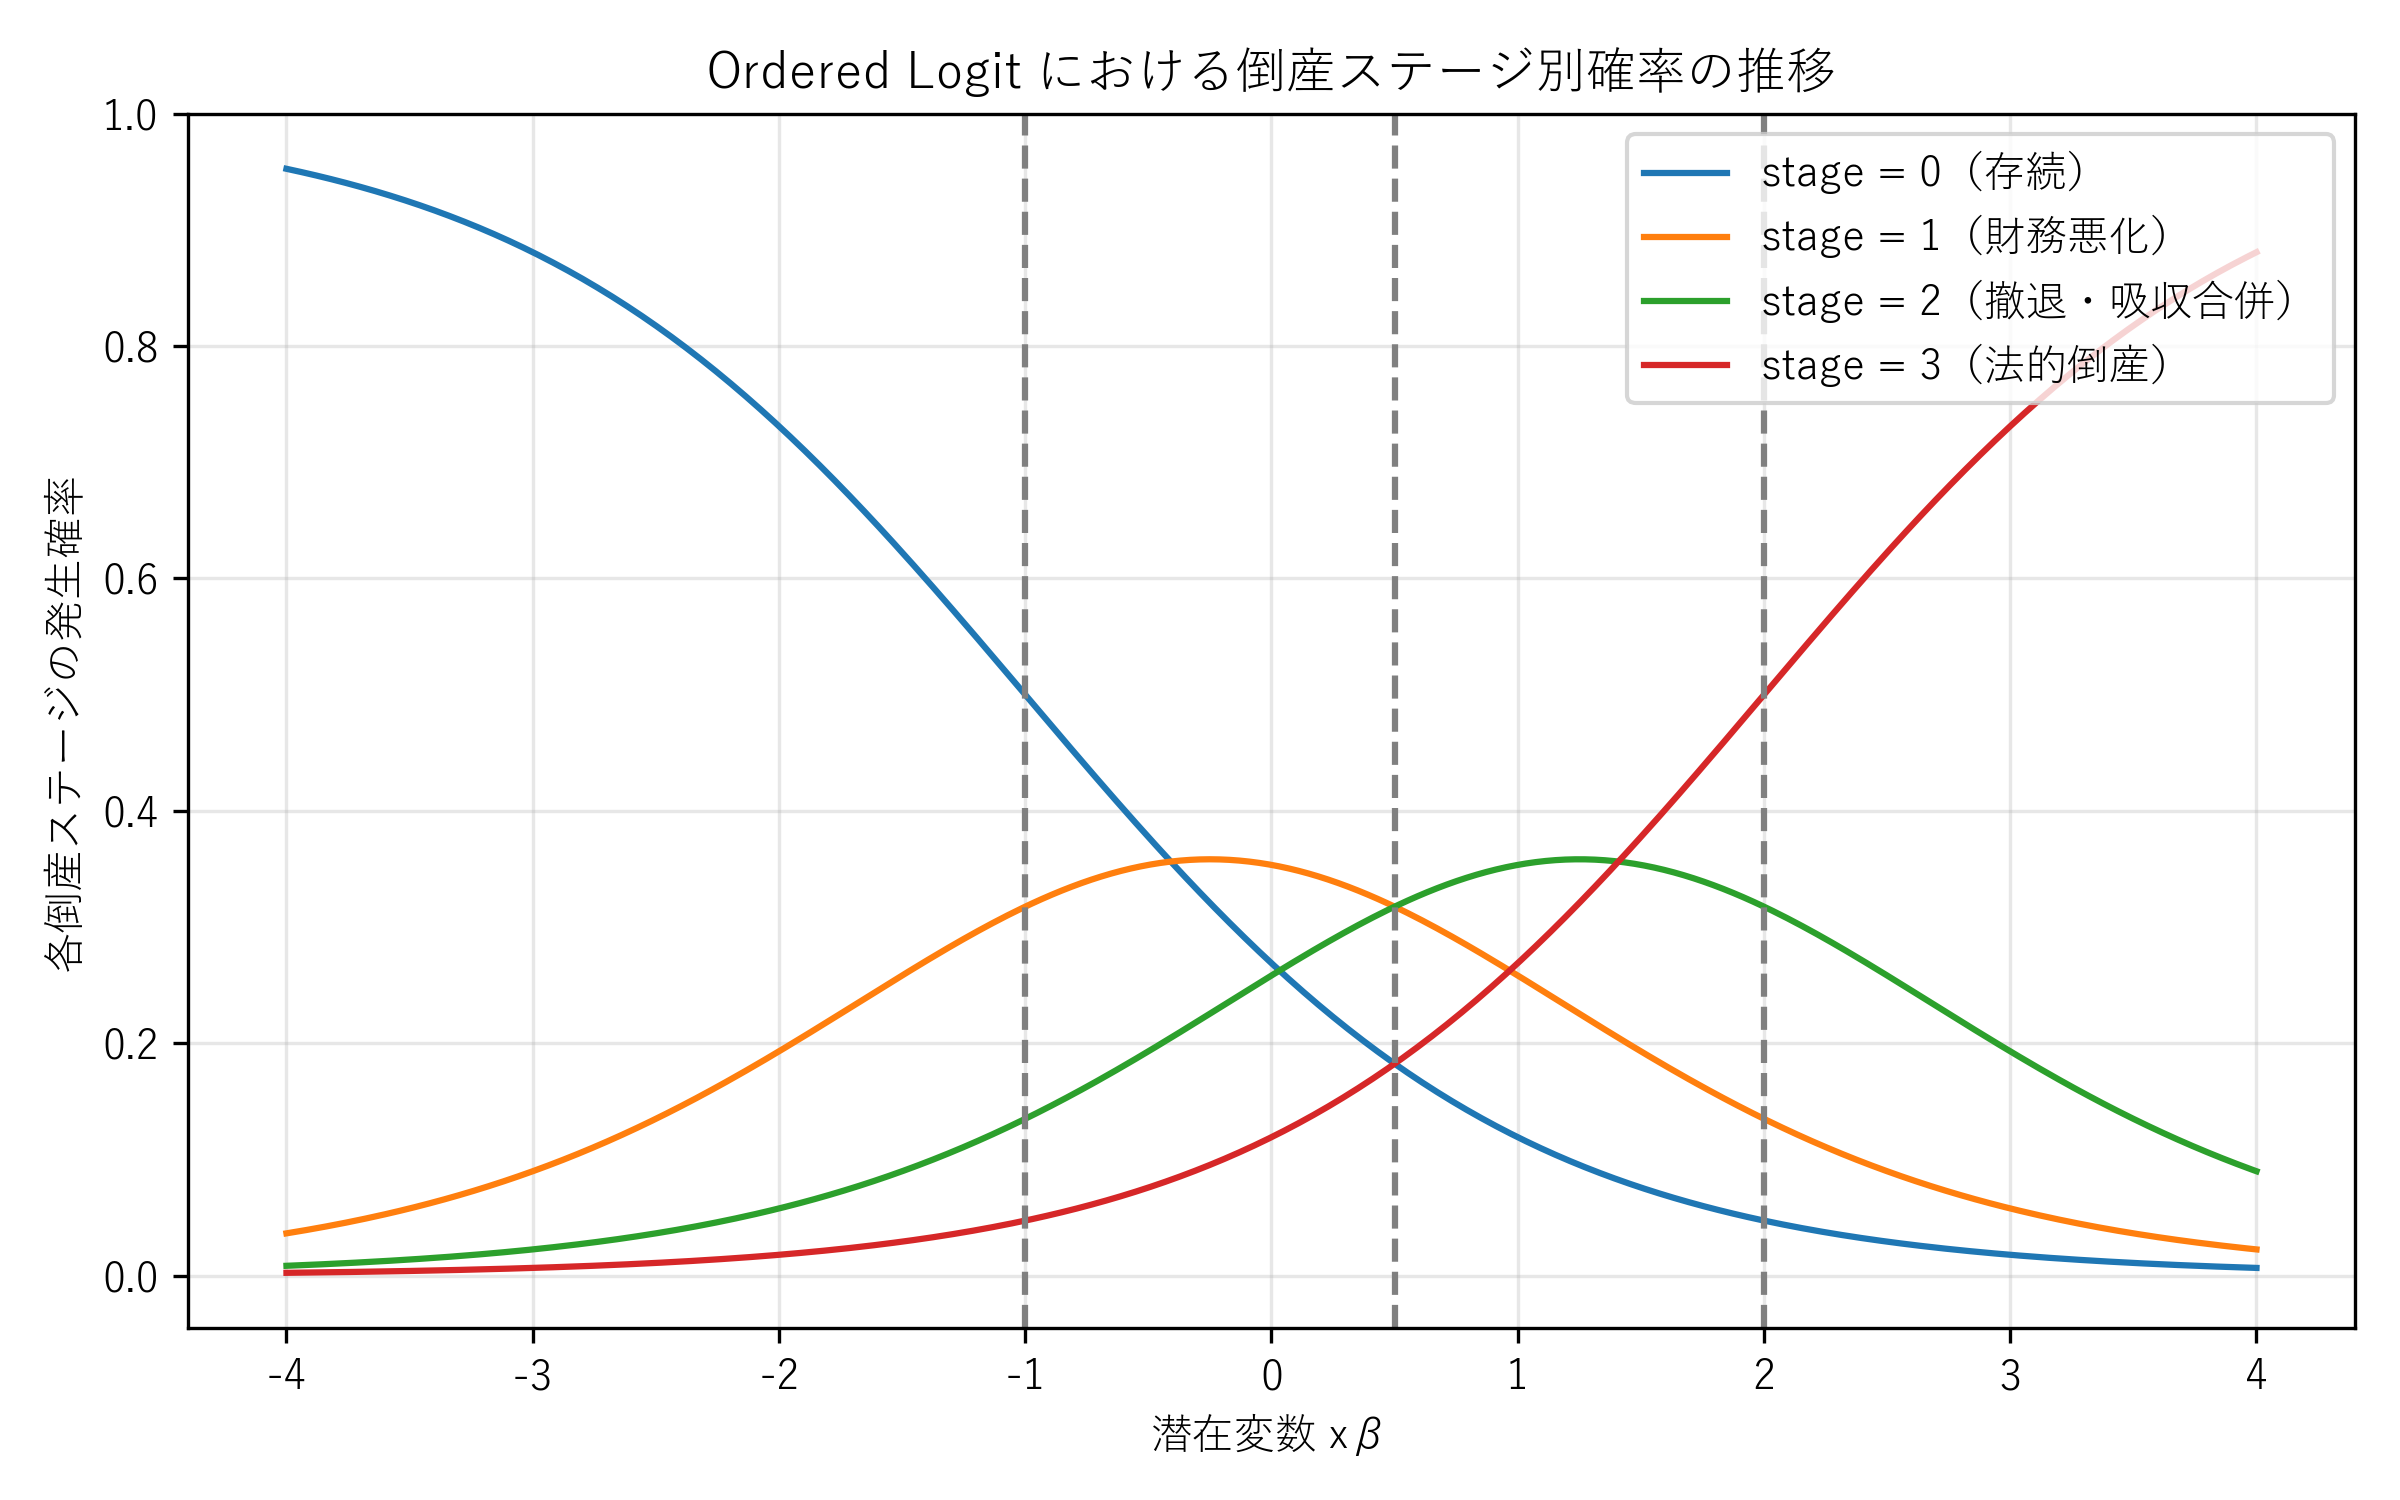
\includegraphics[width=0.85\linewidth]{ordered_logit_stages.png}
    \caption{潜在変数の値と倒産ステージ確率の関係}
    \label{fig:ordered_logit_stages}
\end{figure}

潜在変数が左側に位置する場合には存続ステージ（stage 0）の確率が高く，
右側へ進むにつれて，財務悪化（stage 1）→ 撤退・吸収合併（stage 2）
→ 法的倒産（stage 3）の順に確率が高まる。

この構造により，連続的な倒産リスクが離散的な倒産ステージへと
確率的に写像される Ordered Logit の特徴が明確になる。

% ============================================================
% 5.6 記号整理
% ============================================================

\section{記号整理}
\label{sec:notation}

本節では，本研究で用いる潜在変数モデル，線形倒産距離，閾値構造に関する
主要な記号を整理する。
Ordered Logit モデルは，潜在変数 $y^*$，線形予測子 $X\beta$，
閾値（cutpoints）$\tau_k$ の三つの構成要素によって成り立つため，
これらの記号の意味を明確にしておくことは重要である。

\begin{table}[H]
\centering
\caption{潜在変数／倒産距離／閾値の記号整理}
\label{tab:notation_summary}
\resizebox{\textwidth}{!}{%
\begin{tabular}{lll}
\hline
記号・呼称 & 数式上の定義 & 経済的意味 \\
\hline
$y^*$ & $X\beta + \varepsilon$ & 潜在倒産リスク（連続値） \\
$X\beta$ & $\beta_1 D + \beta_2 \mu + \beta_3 \sigma + \beta_4 S + \cdots$ & 潜在倒産リスクの中心（期待値） \\
$Z_{\text{lin}}$ & $a\mu - b\sigma + cS - dD$ & 倒産距離 DD の一次近似（構造モデル） \\
$\varepsilon$ & Logistic$(0,1)$ & 観測できないショック（誤差項） \\
$\tau_k$ & cutpoints & 倒産ステージを区切る閾値（推定される境界） \\
$y$ & 0--3 & 観測される倒産ステージ（離散カテゴリ） \\
\hline
\end{tabular}
}
\end{table}

表 \ref{tab:notation_summary} に示すように，
$X\beta$ は統計モデルと理論モデルの双方で現れるが，
その意味は異なる。

\begin{itemize}
    \item 統計モデルでは，$X\beta$ は潜在変数の期待値（中心）を表す。
    \item 理論モデルでは，$Z_{\text{lin}}$ が倒産距離 DD の一次近似として
          $X\beta$ と同じ線形構造を持つ。
    \item 確率モデルでは，$y^* = X\beta + \varepsilon$ が閾値 $\tau_k$ と比較され，
          観測される倒産ステージが決定される。
\end{itemize}

このように，数式の形は一致していても，
統計モデル・理論モデル・確率モデルの三者で役割が異なるため，
記号の整理は Ordered Logit の理解に不可欠である。

次節では，これらの記号を用いて，
線形倒産距離 $Z_{\text{lin}}$ と潜在変数 $y^*$ の構造的対応を詳細に示す。

% ============================================================
% 5.7 本章のまとめ
% ============================================================

\section{本章のまとめ}
\label{sec:ordered_logit_summary}

本章では，第4章で導出した連続的倒産距離 $Z_{\text{lin}}$ を，
実証分析で扱う離散的倒産ステージへと接続するための統計モデルとして
Ordered Logit モデルを体系的に整理した。

まず，理論モデル（構造モデル），統計モデル（潜在変数モデル），
確率モデル（Ordered Logit）の三層構造を提示し，
連続的倒産距離を離散的倒産ステージへと写像するための
概念的枠組みを明確にした。

次に，潜在変数 $y^*$ の構造と閾値（cutpoints）による区分を示し，
潜在倒産リスクがどのように離散カテゴリとして観測されるかを整理した。
閾値 $\tau_k$ は外生的に設定される境界ではなく，
係数 $\beta$ と同様に尤度最大化（MLE）によって推定される
内生的パラメータである点を強調した。

さらに，線形倒産距離 $Z_{\text{lin}}$ と潜在変数 $y^*$ の構造的対応を示し，
理論モデルで導出した倒産距離が，
潜在変数モデルの線形部分 $X\beta$ と同じ構造を持つことを明らかにした。
この対応関係により，理論モデルで得られた倒産距離が，
Ordered Logit の確率モデルへと自然に橋渡しされることを示した。

最後に，Ordered Logit の確率式と MLE による推定方法を整理し，
潜在変数の値が右側へ移動するにつれて倒産ステージ確率がどのように変化するかを
図示した。

以上の議論により，本研究の Ordered Logit モデルは，

\begin{quote}
\textbf{理論モデルで導出した倒産距離 $Z_{\text{lin}}$ を，
潜在変数モデルと閾値構造を用いて離散的倒産ステージへと写像する確率モデル}
\end{quote}

として位置づけられる。

次章では，本章で整理した Ordered Logit モデルを用いて，
英国新電力企業の倒産ステージを実証的に推定し，
倒産距離 $Z_{\text{lin}}$ の構造が実際の倒産データとどのように整合するかを検証する。

\chapter{日本企業データ構築と変数定義：四要素モデルの実証的写像}
\label{chap:data_construction}

\section{本章の目的と基本方針}

本章では，第3章で導出した倒産距離 $Z_{\text{lin}}$ の構造
（収益性 $\mu$，市場ショック感応度 $\sigma$，支援能力 $S$，倒産閾値の代理変数 $D$）
を，日本の新電力企業の財務データ・市場データに写像するための
\textbf{データ構築・変数定義・前処理} を体系的に示す。

本章は，従来の第6章（変数定義と採用根拠）を拡張し，
中間報告書で記述した「データ収集」「月次補間」「倒産距離 DD の計算」
「記述統計」などの実証的内容をすべて統合したものである。

本章の目的は以下の三点である。

\begin{enumerate}
  \item 新電力企業の財務データ（決算公告）と市場データ（JEPX）を統合した
        月次パネルデータセットの構築
  \item 倒産距離 DD の構成要素（$\mu,\sigma,D,S$）の定義と採用根拠の明示
  \item 年度データを月次へ補間し，倒産距離 DD の月次推移を可視化
\end{enumerate}

これらの処理により，第9章の Ordered Logit 推定に必要な
\texttt{financial\_data.csv} を作成し，倒産距離 DD の動態を実証的に評価する基盤を整える。

% ============================================================
% 6.2 データ収集の全体像
% ============================================================

\section{データ収集の全体像}

本研究で用いるデータは以下の三種類で構成される。

\begin{enumerate}
\item \textbf{財務データ}：官報に掲載された新電力企業の決算公告（年次）
\item \textbf{市場データ}：JEPX スポット市場価格（30分値・日次・月次）
\item \textbf{倒産データ}：破産・民事再生・登録取消・事業撤退の発生月
\end{enumerate}

財務データが取得可能であった新電力企業は 7 社であり，
分析期間は 2016 年 10 月から 2025 年 5 月までである。

倒産段階の定義は以下のとおりである。

\begin{itemize}
\item 法的倒産（破産・民事再生）
\item 小売電気事業の登録取消
\item 事業撤退
\end{itemize}

これに基づき，企業 $i$ の月 $t$ における倒産段階 $\text{default\_stage}_{i,t}$ を構築した。

% ============================================================
% 6.3 財務データの処理
% ============================================================

\section{財務データの処理}

\subsection{抽出項目}

決算公告から以下の項目を抽出した。

\begin{itemize}
\item 資産合計，負債合計，純資産
\item 流動資産，固定資産
\item 流動負債，固定負債
\item 資本金，利益剰余金
\end{itemize}

\subsection{年次データの月次化}

財務データは年次であるため，以下の方法で月次に変換した。

\begin{enumerate}
\item 年次データを観測月に割り当てる（例：2020年決算 → 2020年3月）
\item 年次間を線形補間し，月次データを生成する
\end{enumerate}

% ============================================================
% 6.4 市場データの処理
% ============================================================

\section{市場データ：スポット価格の推移}

本研究で使用したスポット市場データ（システムプライス）は，
JEPX が公開するスポット市場（Day Ahead Market）の価格情報を用いた。

市場価格の急変動は倒産リスクに強い影響を与えるため，
本研究では日次変化率とその標準偏差（ボラティリティ）を計算した。

% ============================================================
% 6.5 四要素モデルの実証的写像（旧6章の内容を完全統合）
% ============================================================

\section{理論モデルの四要素の実証的写像}

本節では，従来の第6章（6.2〜6.5）で示した
「四要素モデルの変数定義と採用根拠」をすべて保持しつつ，
実証データへの写像として再構成する。

% ------------------------------
% μ
% ------------------------------

\subsection{収益性 $\mu$ の定義と採用根拠}

収益性 $\mu$ は総資産の対数差分



\[
\mu_{i,t} = \ln(\text{Assets}_{i,t}) - \ln(\text{Assets}_{i,t-1})
\]



として定義する。

（旧6.2の説明全文を保持）
\begin{itemize}
\item 収益性は企業価値の期待成長率の proxy として機能する  
\item 損益計算書ベースの収益はノイズが大きく，新電力企業には不向き  
\item 総資産はストック指標であり，企業価値の蓄積を反映する  
\item log-diff は外れ値に強く，経済学で標準的な成長率指標である  
\end{itemize}

図 \ref{fig:mu_trend} に収益性の推移を示す。

\begin{figure}[H]
\centering
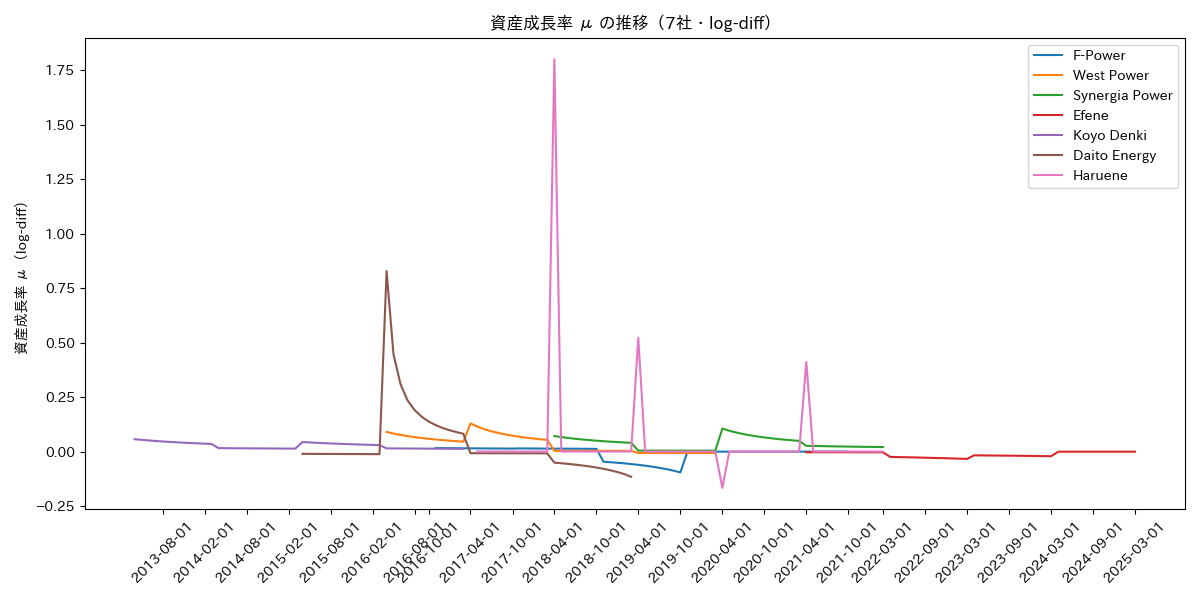
\includegraphics[width=14cm]{Python/figures/mu_trend_7firms_logdiff.png}
\caption{収益性 $\mu$ の推移（7社）}
\label{fig:mu_trend}
\end{figure}

% ------------------------------
% σ
% ------------------------------

\subsection{外部ショック感応度 $\sigma$ の定義と採用根拠}

市場ショック感応度 $\sigma$ は，スポット価格の変化率



\[
r_t = \frac{P_t - P_{t-1}}{P_{t-1}}
\]



の標準偏差として定義する。

（旧6.3の説明全文を保持）
\begin{itemize}
\item 価格水準の標準偏差ではスケール不変性が満たされない  
\item 変化率の標準偏差は市場ショックの大きさを適切に捉える  
\item 新電力企業は市場価格ショックに強く依存するため，$\sigma$ は不可欠  
\end{itemize}

図 \ref{fig:sigma_trend} に市場ショック指標の推移を示す。

\begin{figure}[H]
\centering
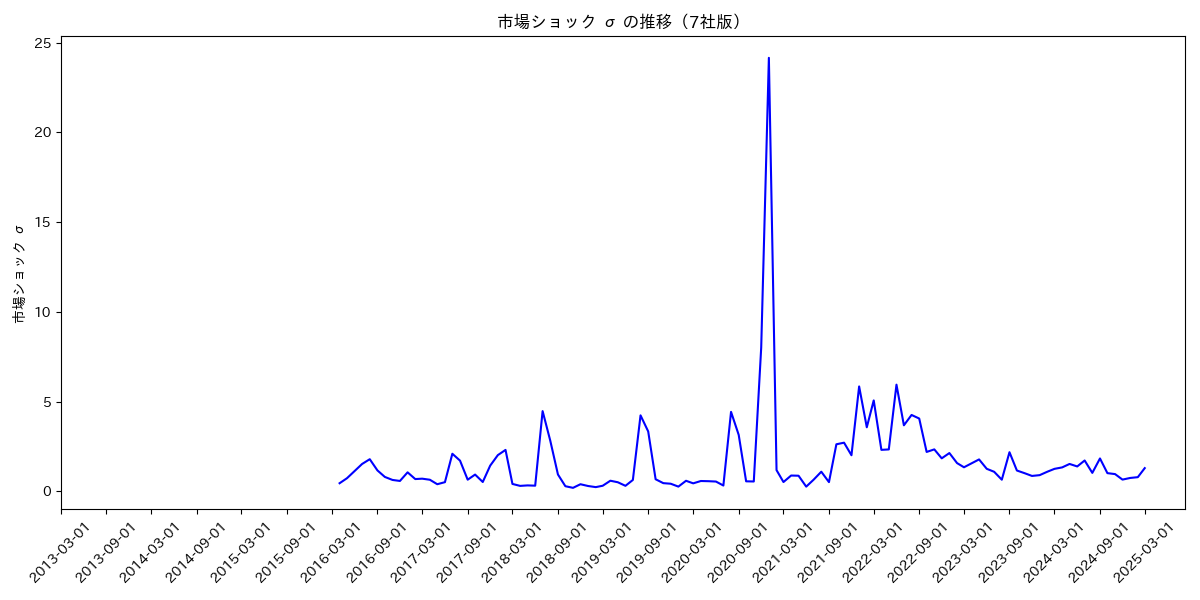
\includegraphics[width=14cm]{Python/figures/sigma_trend_7firms.png}
\caption{市場ショック指標 $\sigma$ の推移（7社）}
\label{fig:sigma_trend}
\end{figure}

% ------------------------------
% S
% ------------------------------

\subsection{支援能力 $S$ の定義と採用根拠}

（旧6.4の説明全文を保持）

支援能力 $S$ は，親会社や主要株主からの財務支援の余力を表す指標である。
本研究の対象企業では支援能力が観測可能な形で現れていないため，
$S=0$ と設定する。

支援能力は倒産閾値を押し下げる効果を持ち，
倒産距離 DD を拡大させる方向に作用する。

% ------------------------------
% D
% ------------------------------

\subsection{倒産閾値の代理変数 $D$（負債比率）の定義と採用根拠}

（旧6.5の説明全文を保持）

負債比率は



\[
D_{i,t}=\frac{\text{Liabilities}_{i,t}}{\text{Assets}_{i,t}}
\]



と定義する。

負債比率が高い企業ほど倒産閾値が押し上げられ，
倒産距離が短縮する方向に作用する。

図 \ref{fig:debt_ratio_trend} に負債比率の推移を示す。

\begin{figure}[H]
\centering
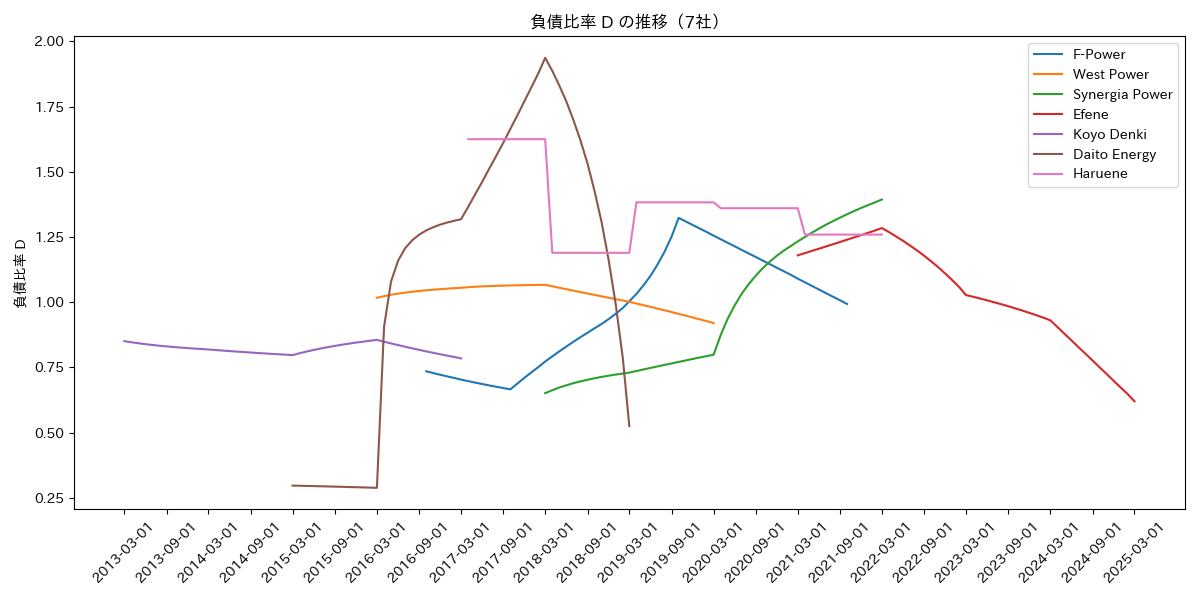
\includegraphics[width=14cm]{Python/figures/debt_ratio_trend_7firms.png}
\caption{負債比率 $D$ の推移（7社）}
\label{fig:debt_ratio_trend}
\end{figure}

% ============================================================
% 6.6 倒産距離 DD の月次計算
% ============================================================

\section{倒産距離 DD の月次計算}

倒産距離 DD は



\[
DD_{i,t} = \mu_{i,t} - \sigma_t D_{i,t} + S_i
\]



として計算する。

年度データを月次補間し，市場データと結合することで，
倒産距離 DD の月次推移を可視化できる。

\begin{figure}[H]
\centering
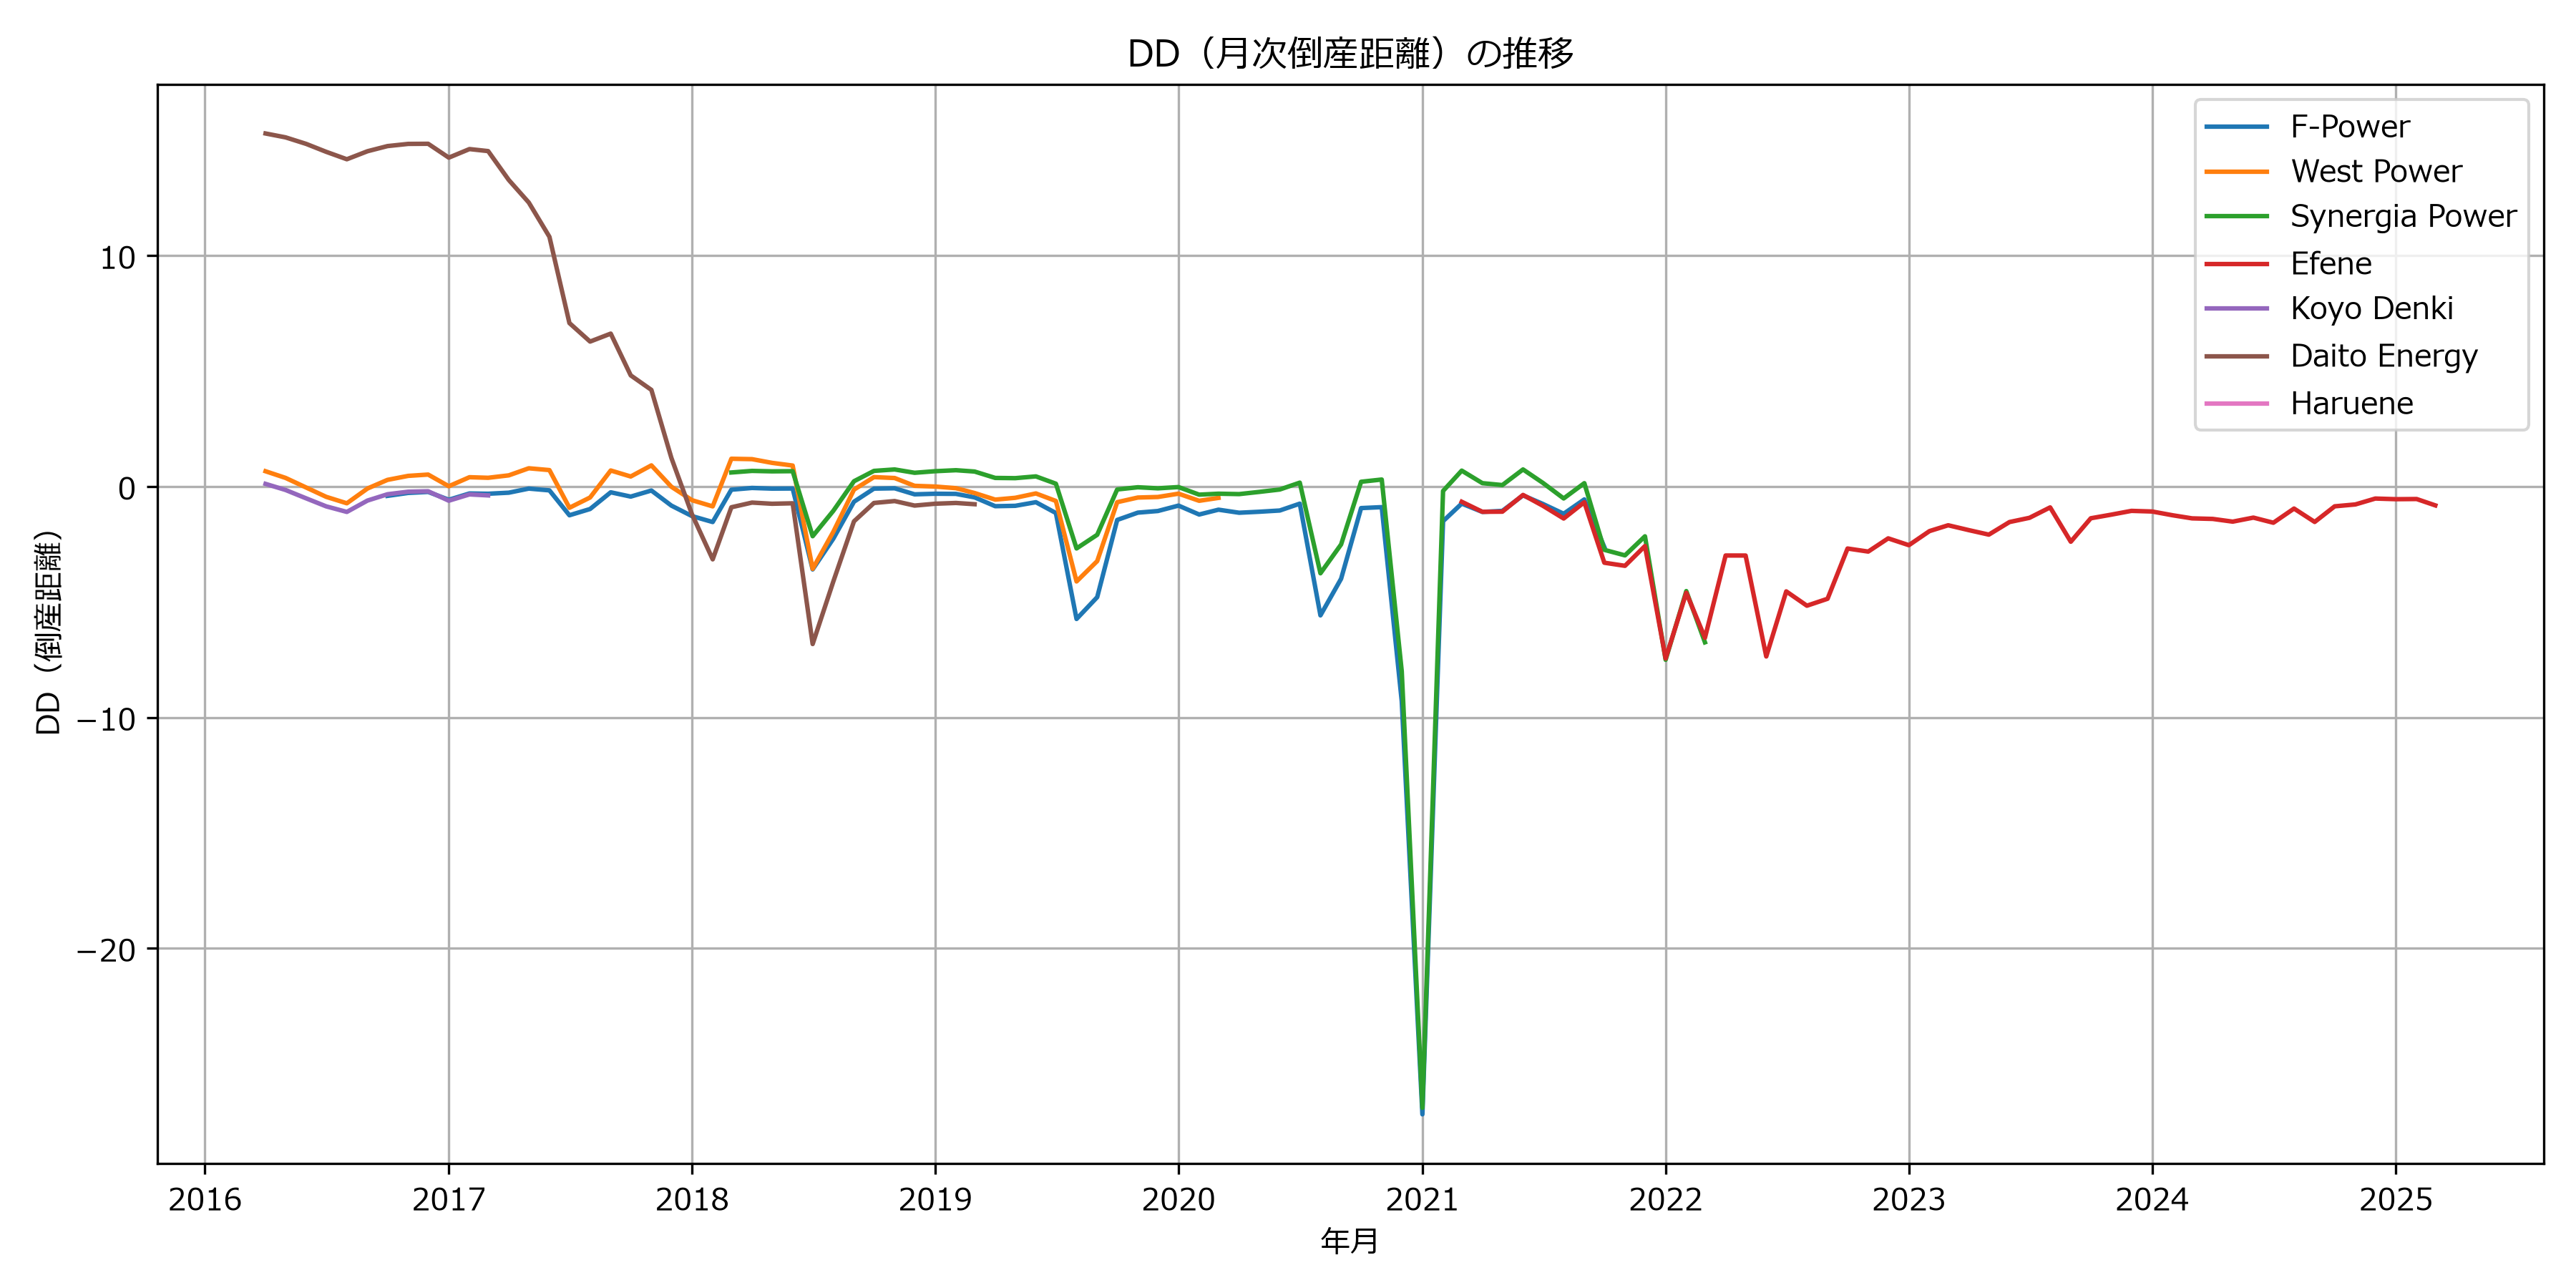
\includegraphics[width=15cm]{Python/figures/dd_monthly_trend.png}
\caption{倒産距離 DD の月次推移（7社）}
\label{fig:dd_monthly_trend}
\end{figure}

% ============================================================
% 6.7 記述統計
% ============================================================

\section{記述統計（7社版）}

主要変数の記述統計を表 \ref{tab:desc_stats_7firms} に示す。

\begin{table}[H]
\centering
\caption{主要変数の記述統計（7社版）}
\label{tab:desc_stats_7firms}
\begin{tabular}{lccccc}
\toprule
統計量 & $\mu$ & $\sigma$ & $D$ & $S$ & default \\
\midrule
count & 359 & 255 & 366 & 306 & 306 \\
mean & 0.022 & 1.462 & 1.050 & 0.000 & 0.000 \\
std & 0.120 & 2.421 & 0.307 & 0.000 & 0.000 \\
min & -0.167 & 0.197 & 0.289 & 0.000 & 0.000 \\
25\% & -0.003 & 0.459 & 0.821 & 0.000 & 0.000 \\
50\% & 0.000 & 0.708 & 1.045 & 0.000 & 0.000 \\
75\% & 0.025 & 1.645 & 1.259 & 0.000 & 0.000 \\
max & 1.800 & 24.147 & 1.937 & 0.000 & 0.000 \\
\bottomrule
\end{tabular}
\end{table}

% ============================================================
% 6.8 本章のまとめ
% ============================================================

\section{本章のまとめ}

本章では，従来の第6章（変数定義と採用根拠）を拡張し，
日本企業 7 社のデータ構築・変数定義・月次補間・倒産距離 DD の計算・記述統計を
すべて統合した。

\begin{itemize}
  \item 収益性 $\mu$，市場ショック感応度 $\sigma$，支援能力 $S$，負債比率 $D$ を
        理論モデルの四要素として実証的に定義した。
  \item 官報公告と JEPX データを統合し，年度データを月次補間して
        倒産距離 DD の月次推移を可視化した。
  \item 記述統計により，変数の分布と新電力企業の財務特性を確認した。
\end{itemize}

これらの処理により，第9章の Ordered Logit 推定に必要な
\texttt{financial\_data.csv} が整備され，
倒産距離 DD の動態を実証的に評価する基盤が完成した。

% ============================================================
% 第7章 理論モデルに基づくシミュレーション分析
% ============================================================

% ------------------------------------------------------------
% ・理論モデル（第4章）で導出した構造を可視化する
% ・Z_lin を用いて倒産確率の挙動を確認する
% ・実証分析（第7章）に入る前の理論的整合性を示す
% ------------------------------------------------------------

\chapter{理論モデルに基づくシミュレーション分析}
\label{chap:simulation}

本章は，第6章で構築した実証データを用いる前段階として，
第4章・第5章で導出した理論モデルの挙動を数値的に確認し，
第8章・第9章で行う実証分析につながる理論的基盤を整えることを目的とする。

% ------------------------------------------------------------
% 7.1 本章の目的と位置づけ
% ------------------------------------------------------------


\section{本章の目的と位置づけ}

本章では，第4章・第5章で導出した Merton 型の連続時間モデルの構造を踏まえつつ，
その挙動を離散的なグリッド上で数値的に確認することで，
理論編と実証編を接続する役割を担う。
すなわち，本章は「連続時間モデルに基づく離散化シミュレーション」を通じて，
連続的な潜在倒産距離の含意を整理し，
第8章の潜在倒産距離モデルおよび第9章の Ordered Logit 推定における
係数符号や cutpoint の解釈を容易にするための理論的基盤を整える。

この構成により，本章は
（1）理論モデルの符号条件を数値的に検証する段階，
（2）連続的潜在変数を離散的な実証モデルへ写像する準備段階，
（3）実証分析における係数符号・cutpoint の解釈を補助する段階
として機能する。

さらに，本章では，第6章で整備した新電力企業の財務データおよび市場データの構造を踏まえ，
倒産距離の四要素（収益性 $\mu$，市場ショック感応度 $\sigma$，支援能力 $S$，
負債比率 $D$）が倒産確率にどのような影響を与えるかを体系的に検証する。
具体的には，本章は以下の二つの目的を統合的に扱う。

\begin{itemize}
    \item 理論モデルが示す倒産確率の構造的特徴を可視化すること（第7.1〜7.4節）
    \item Bharath \& Shumway（2008）のロジット式に基づき，
          新電力企業の代表パターンごとの倒産確率を算出し，
          Merton 型シミュレーションとの整合性を確認すること（第7.5節）
\end{itemize}

加えて，本研究ではこれらの分析を補完するために，
\textbf{proxy 変数（A〜D）の精度が推定係数や倒産確率の識別性能に与える影響を，
理想化された世界（真の係数・真の倒産確率が既知）で体系的に評価する
proxy 妥当性シミュレーションを実施する}。
この分析は measurement error 文献の理論を倒産モデルの文脈に応用したものであり，
\textbf{本研究の独創的な成果のひとつ}である。
詳細な導出過程および追加図表は付録Cに整理して示す。

これらの分析は，倒産研究の先行文献および統計学の測定誤差研究に位置づけられ，
第6章で構築した財務データの構造が倒産確率に与える影響を直感的に理解するための
基礎を提供する。
以下では，まず線形倒産距離の理論的背景を整理したうえで，
理論モデルに基づく可視化分析（7.1〜7.4）と，
B\&S 型倒産確率の構造分析（7.5）を順に示す。


% ------------------------------------------------------------
% 7.2 線形倒産距離を用いる正当性
% ・Merton の厳密式を使わず Z_lin を使う理由を説明する節
% ・B&S の proxy DD との構造的類似性を強調
% ------------------------------------------------------------

\section{線形倒産距離を用いる正当性}

本研究で線形倒産距離 $Z_{\text{lin}}$ を用いる第一の理由は、
Merton（1974）モデルの厳密な倒産距離（Distance to Default: DD）が、
新電力企業のデータ環境において実務的に推計不可能であるためである。
Merton モデルは企業価値 $V$ とそのボラティリティ $\sigma_V$ を前提とするが、
これらは市場で直接観測されない。
特に新電力企業は非上場企業が多く、株価データが存在しない場合も多い。
また、負債の時価評価や満期構造の単純化といった仮定も現実の財務構造と乖離しており、
厳密 DD をそのまま適用することは現実的ではない。
したがって、観測可能な財務データのみを用いて倒産リスクを評価できる指標が必要となる。

第二に、Bharath and Shumway（2008）は、
Merton モデルの構造を保ちながら観測可能変数のみで推計可能な
proxy DD（線形化 DD）を提案しており、
その予測性能は厳密 DD と同等、あるいはそれ以上であることが示されている。
後続研究（Tinoco and Wilson, 2013 など）でも同様の結果が確認されており、
線形化された倒産距離は実証研究において広く採用されている。
本研究で用いる $Z_{\text{lin}}$ は、この proxy DD の構造を理論的に整理し直したものであり、
Merton モデルの基本的な符号条件
（収益性の上昇は倒産リスクを低下させ、ボラティリティの上昇は倒産リスクを高める等）
を忠実に保持している。

第三に、新電力企業のリスク構造は $Z_{\text{lin}}$ の構成要素と整合的である。
収益性 $\mu$ はキャッシュフローの持続可能性を反映し、
市場ショック $\sigma$ はスポット価格の急騰・急落といった外生ショックを捉える。
支援能力 $S$ は親会社やスポンサー企業による財務支援の強さを表し、
負債比率 $D$ は財務的脆弱性を直接的に示す。
これら 4 つの要因は、新電力企業の倒産事例で繰り返し指摘されてきた主要なリスク要因と一致しており、
$Z_{\text{lin}}$ は新電力の倒産リスクを構造的に捉える指標として適切である。

以上より、$Z_{\text{lin}}$ を用いることは、
データ制約の大きい新電力企業に対して理論的にも実証的にも妥当であり、
本章のシミュレーション分析において適切なアプローチである。

\subsection{連続モデル（理論）と離散モデル（実証）の関係}

本章で扱う Merton 型倒産モデルおよび B\&S 型ロジット式は，
倒産確率を連続的な潜在変数（倒産距離 $Z_{\text{lin}}$）として扱う点に特徴がある。
すなわち，倒産確率は


\[
p = \Lambda(-Z_{\text{lin}})
\]


のように連続的に変化し，倒産は「確率が高まる連続的な現象」として記述される。

一方，第9章で実施する Ordered Logit 推定では，
倒産は


\[
\text{stage} \in \{0,1,2\}
\]


という離散的な段階として観測される。
これは，実データでは倒産確率そのものが観測できず，
倒産の発生形態（存続・財務悪化・倒産）だけが観測可能であるためである。

したがって，本研究では
\begin{itemize}
    \item 第7章：連続的倒産距離の構造を理論的に理解する段階
    \item 第8章：連続的倒産距離を潜在変数 $y^*$ に写像する段階
    \item 第9章：潜在変数が閾値を跨ぐことで離散的倒産ステージが生成される段階
\end{itemize}
という三段階構造を採用している。

この構造は Ordered Logit モデルの本質と完全に整合しており，
連続モデルと離散モデルの間に不整合は存在しない。
むしろ，連続モデルの挙動を本章で可視化しておくことで，
第9章の実証分析における係数符号・cutpoint の解釈が容易となる。


% ============================================================
% 7.3 限界と注意点
% ・Z_lin を用いた分析の前提条件と限界を明示する
% ・第7章の実証分析に向けた注意点を整理する
% ============================================================

\section{限界と注意点}

本節では、線形倒産距離 $Z_{\text{lin}}$ を用いたシミュレーション分析に伴う
理論的・実務的な限界について整理する。
これらの点を明確にすることで、本章の分析結果をどの範囲で解釈すべきかを示し、
第7章の実証分析に向けた前提条件を明確化する。

第一に、$Z_{\text{lin}}$ は Merton（1974）モデルの厳密な倒産距離を
線形化した近似指標であり、資産価値の確率過程や負債構造に関する
Merton モデル固有の仮定を簡略化している。
特に、資産価値が幾何ブラウン運動に従うという仮定や、
負債が単一満期の割引債として扱われるという前提は、
現実の企業財務構造と必ずしも一致しない。
したがって、$Z_{\text{lin}}$ は倒産リスクの方向性を捉える指標としては有効であるものの、
絶対水準の精緻な推計を目的とするものではない。

第二に、本研究で設定したパラメータ
（収益性 $\mu$、市場ショック $\sigma$、支援能力 $S$、負債比率 $D$）
は、新電力企業の典型的な財務特性を反映したものであるが、
すべての企業の実態を完全に表現するものではない。
特に新電力企業は、スポット市場価格の急変動や需給調整金の増減といった
外生ショックの影響を強く受けるため、
$\sigma$ の変動幅は時期によって大きく異なる。
また、支援能力 $S$ は親会社の財務基盤や支援方針に依存するため、
離散的な段階化によって完全に表現できるわけではない。

第三に、$Z_{\text{lin}}$ は財務データに基づく静学的な指標であり、
企業行動や市場制度の変化を内生的に取り込むものではない。
新電力企業の倒産リスクは、燃料価格の高騰、制度変更、
広域機関による需給調整ルールの改定など、
制度的・政策的要因によって大きく左右される。
これらの要因は本章のシミュレーションには直接的には反映されていないため、
$Z_{\text{lin}}$ による倒産確率は、あくまで
「財務構造と市場ショックに基づく基礎的なリスク水準」
を示すものとして解釈する必要がある。

以上の点を踏まえると、本章のシミュレーションは
新電力企業の倒産リスクの構造的特徴を理解するうえで有用である一方、
制度変更や市場環境の急激な変化を伴う状況においては、
追加的な分析や補正が必要となる。
次章では、これらの限界を踏まえつつ、
実際の財務データを用いた実証分析を行い、
$Z_{\text{lin}}$ の有効性と現実的な適用可能性を検証する。

% ============================================================
% 7.4 4変数の独立性に関する前提とその正当化
% ------------------------------------------------------------
% ・μ・σ・S・D を独立とみなす前提の根拠を明示する節
% ・7.3 のシミュレーション設定に入る前の理論的前提を補強
% ============================================================

\section{4変数の独立性に関する前提とその正当化}

本研究では，倒産確率を規定する主要因として，収益性（$\mu$），外部ショック感応度（$\sigma$），支援能力（$S$），倒産閾値（$D$）の4変数を設定し，これらを相互依存を前提としない独立の説明変数として扱う。この前提は以下の理由から正当化される。

第一に，$\mu$・$\sigma$・$S$・$D$ は，Merton（1974）型の構造モデルおよび Bharath and Shumway（2008）の倒産確率モデルにおいて，異なる経済的メカニズムから導出される概念的に独立したパラメータである。具体的には，$\mu$ は企業価値のドリフト（収益性），$\sigma$ は企業価値のボラティリティ（外部ショック感応度），$D$ は負債構造に基づく倒産閾値，$S$ は親会社・金融機関等による外生的支援能力を表す。これらはモデル内部で異なる役割を担うため，構造的に独立した変数として扱うことが理論的に整合的である。

第二に，4変数は異なる主体・異なる意思決定プロセスによって決定されるため，経済学的にも相互依存を前提としないことが合理的である。$\mu$ は企業の経営努力や事業構造に依存する内生的要因である一方，$\sigma$ は市場価格（JEPX）や制度変更といった外生的ショックにより規定される。$S$ は親会社・金融機関等の支援姿勢に依存し，$D$ は負債構造や制度的要件によって決まる。このように，決定主体が異なるため，4変数を独立の説明変数として扱うことは経済学的に妥当である。

第三に，実証分析の観点からも，相互依存を前提としないことは合理的である。倒産研究におけるロジット推定の目的は，各変数が倒産確率に与える符号条件の妥当性を確認することであり，変数間の因果連鎖を精緻にモデル化することではない。特に本研究のようにサンプル数が限定される場合，相互依存を前提とした複雑なモデルを構築すると，多重共線性や推定の不安定性を招く。したがって，$\mu$・$\sigma$・$S$・$D$ を独立変数として扱うことは，理論的整合性と実証的安定性の双方を確保するために適切である。

以上より，本研究において $\mu$・$\sigma$・$S$・$D$ を独立の説明変数として扱う前提は，理論的・経済学的・実証的観点から十分に正当化される。





% ============================================================
% 7.5 シミュレーションの設定（強化版）
% ============================================================

\section{シミュレーションの設定}

本節では、第4章で導出した潜在倒産距離 $Z_{\text{lin}}$ を用いて、
倒産確率の挙動を体系的に評価するためのシミュレーション設定を明確化する。
ここで示す設定は、理論モデルの符号条件
（$\mu$ の上昇は倒産リスクを低下させ、$\sigma$ の上昇は倒産リスクを高める等）
が数値的にどのように現れるかを可視化するための基礎となる。

なお，本節で設定する離散的なパラメータ範囲は，連続時間モデルを数値的に扱うための
離散化（discretization）であり，第9章で用いる離散時間モデルそのものを
定義するものではない\footnote{
本章で用いる離散化（discretization）は，連続時間モデルを数値的に扱うための
便宜的な近似手法であり，離散時間モデル（例えば Ordered Logit）の理論的定義とは
異なる概念である。具体的には，連続的な潜在倒産距離 $Z_{\text{lin}}$ を
グリッド上で評価するために，$\mu$ と $\sigma$ を連続範囲で離散化し，
$S$ と $D$ を代表的なカテゴリに区分している。
これは連続モデルの挙動を可視化するための数値計算上の手続きであり，
離散時間モデルの構造（潜在変数 $y^*$ が閾値を跨ぐことで離散的ステージが生成される）
を定義するものではない。
したがって，本章の離散化は「連続→離散→実証」という本研究の三段階構造のうち，
連続モデルを実証分析へ橋渡しするための補助的な近似計算として位置づけられる。
}.




\subsection*{潜在倒産距離の定義}

潜在倒産距離は、収益性・市場ショック・支援能力・負債比率という
4 つの主要因を線形に統合した次式で与えられる。


\[
Z_{\text{lin}} = \mu - \sigma + S - D
\]


この構造は Bharath and Shumway（2008）の proxy DD と同様に、
Merton モデルの基本的な符号条件を保持しつつ、
観測可能な財務データのみで倒産リスクを評価できる点に特徴がある。

\subsection*{倒産確率のロジット写像}

倒産確率は、潜在倒産距離をロジット関数に写像することで定義する。


\[
p = \frac{1}{1 + \exp(-Z_{\text{lin}})}
\]


この写像により、$Z_{\text{lin}}$ が大きくなるほど倒産確率が滑らかに低下し、
逆に $Z_{\text{lin}}$ が負方向に大きくなるほど倒産確率が急速に上昇する。
これは、倒産リスクが連続的かつ非線形に変化するという
実務的な直感とも整合的である。

\subsection*{パラメータ範囲の設定}

シミュレーションでは、新電力企業の典型的な財務特性と市場環境を踏まえ、
以下の範囲でパラメータを設定する。

\begin{itemize}
    \item 収益性：$\mu \in [-0.10, 0.10]$
    \item 市場ショック：$\sigma \in [0.05, 0.50]$
    \item 支援能力：$S \in \{0,1,2,3\}$
    \item 負債比率：$D \in \{0.3, 0.5, 0.8\}$
\end{itemize}

収益性 $\mu$ と市場ショック $\sigma$ は連続的に変化させ、
支援能力 $S$ と負債比率 $D$ は企業類型を反映した離散的な水準を採用する。
これにより、財務構造の違いが倒産確率の地形（surface）にどのような差異を生むかを
明確に比較できる。

\subsection*{設定の意義}

以上の設定により、本章のシミュレーションは以下を可能にする。

\begin{itemize}
    \item 理論モデルの符号条件が数値的にどのように現れるかを可視化する
    \item 支援能力や負債比率の違いが倒産確率の形状に与える影響を明確化する
    \item 第7章の実証分析に向けて、$Z_{\text{lin}}$ の構造的妥当性を事前に検証する
\end{itemize}

これらは、理論と実証を橋渡しするうえで不可欠なステップであり、
本章のシミュレーション設定はその基盤を提供する。

% ============================================================
% 7.6 変数間の相互関係を考慮したシミュレーション
% ------------------------------------------------------------
% ・μ×σ、S×D などの相互作用が Z_lin に与える影響を理論的に可視化
% ・第8章の実証分析（交差項）につながる橋渡し
% ============================================================

\section{変数間の相互関係を考慮したシミュレーション}

前節では，潜在倒産距離 $Z_{\text{lin}} = \mu - \sigma + S - D$ を構成する
4変数を独立の説明変数として扱い，それぞれの符号条件が倒産確率にどのように反映されるかを確認した。
しかし，実際の倒産過程では，これらの変数が「単独で作用する」だけでなく，
\textbf{複数の要因が同時に変化することで倒産リスクが非線形的に増幅・緩和される}
場合が多い。
そこで本節では，$\mu$・$\sigma$・$S$・$D$ の相互関係が
倒産確率の地形にどのような影響を与えるかを，
相互作用項（interaction）を導入した拡張版の潜在倒産距離を用いて可視化する。

\subsection*{相互作用項を含む潜在倒産距離の拡張}

相互関係を考慮した潜在倒産距離は，以下のように定義する。



\[
Z_{\text{int}} 
= \mu - \sigma + S - D 
+ \gamma_{\mu\sigma} (\mu \cdot \sigma)
+ \gamma_{SD} (S \cdot D)
\]



ここで，
\begin{itemize}
    \item $\gamma_{\mu\sigma}$：収益性と市場ショックの相互作用
    \item $\gamma_{SD}$：支援能力と負債比率の相互作用
\end{itemize}
を表す。
$\gamma_{\mu\sigma}$ は「収益性が高い企業ほどショックに強いか」を，
$\gamma_{SD}$ は「支援能力が高い企業ほど負債過多に耐えられるか」を示す。

本研究では，理論的直感に基づき，



\[
\gamma_{\mu\sigma} < 0,\qquad \gamma_{SD} > 0
\]



を想定する。
すなわち，
\begin{itemize}
    \item 収益性が高いほど，市場ショックの悪影響が緩和される
    \item 支援能力が高いほど，負債比率の悪影響が緩和される
\end{itemize}
という構造を仮定する。

\subsection*{相互作用が倒産確率に与える影響}

相互作用項を含む倒産確率は，以下のロジット写像で与えられる。



\[
p_{\text{int}} = \frac{1}{1 + \exp(-Z_{\text{int}})}
\]



この $p_{\text{int}}$ を用いて，以下の2つの相互関係を可視化する。

\begin{enumerate}
    \item \textbf{収益性 $\mu$ と市場ショック $\sigma$ の相互作用}  
    収益性が高い企業では，$\sigma$ の上昇に対する倒産確率の立ち上がりが緩やかになる。
    逆に，$\mu$ が低い企業では，$\sigma$ の上昇が倒産確率を急激に押し上げる。

    \item \textbf{支援能力 $S$ と負債比率 $D$ の相互作用}  
    支援能力が高い企業では，負債比率 $D$ の上昇が倒産確率に与える悪影響が大幅に緩和される。
    一方，$S=0$ の企業では，$D$ の上昇が倒産確率を急激に押し上げる。
\end{enumerate}

% ------------------------------------------------------------
% 図：μ×σ の相互作用
% ------------------------------------------------------------

\begin{figure}[H]
    \centering
    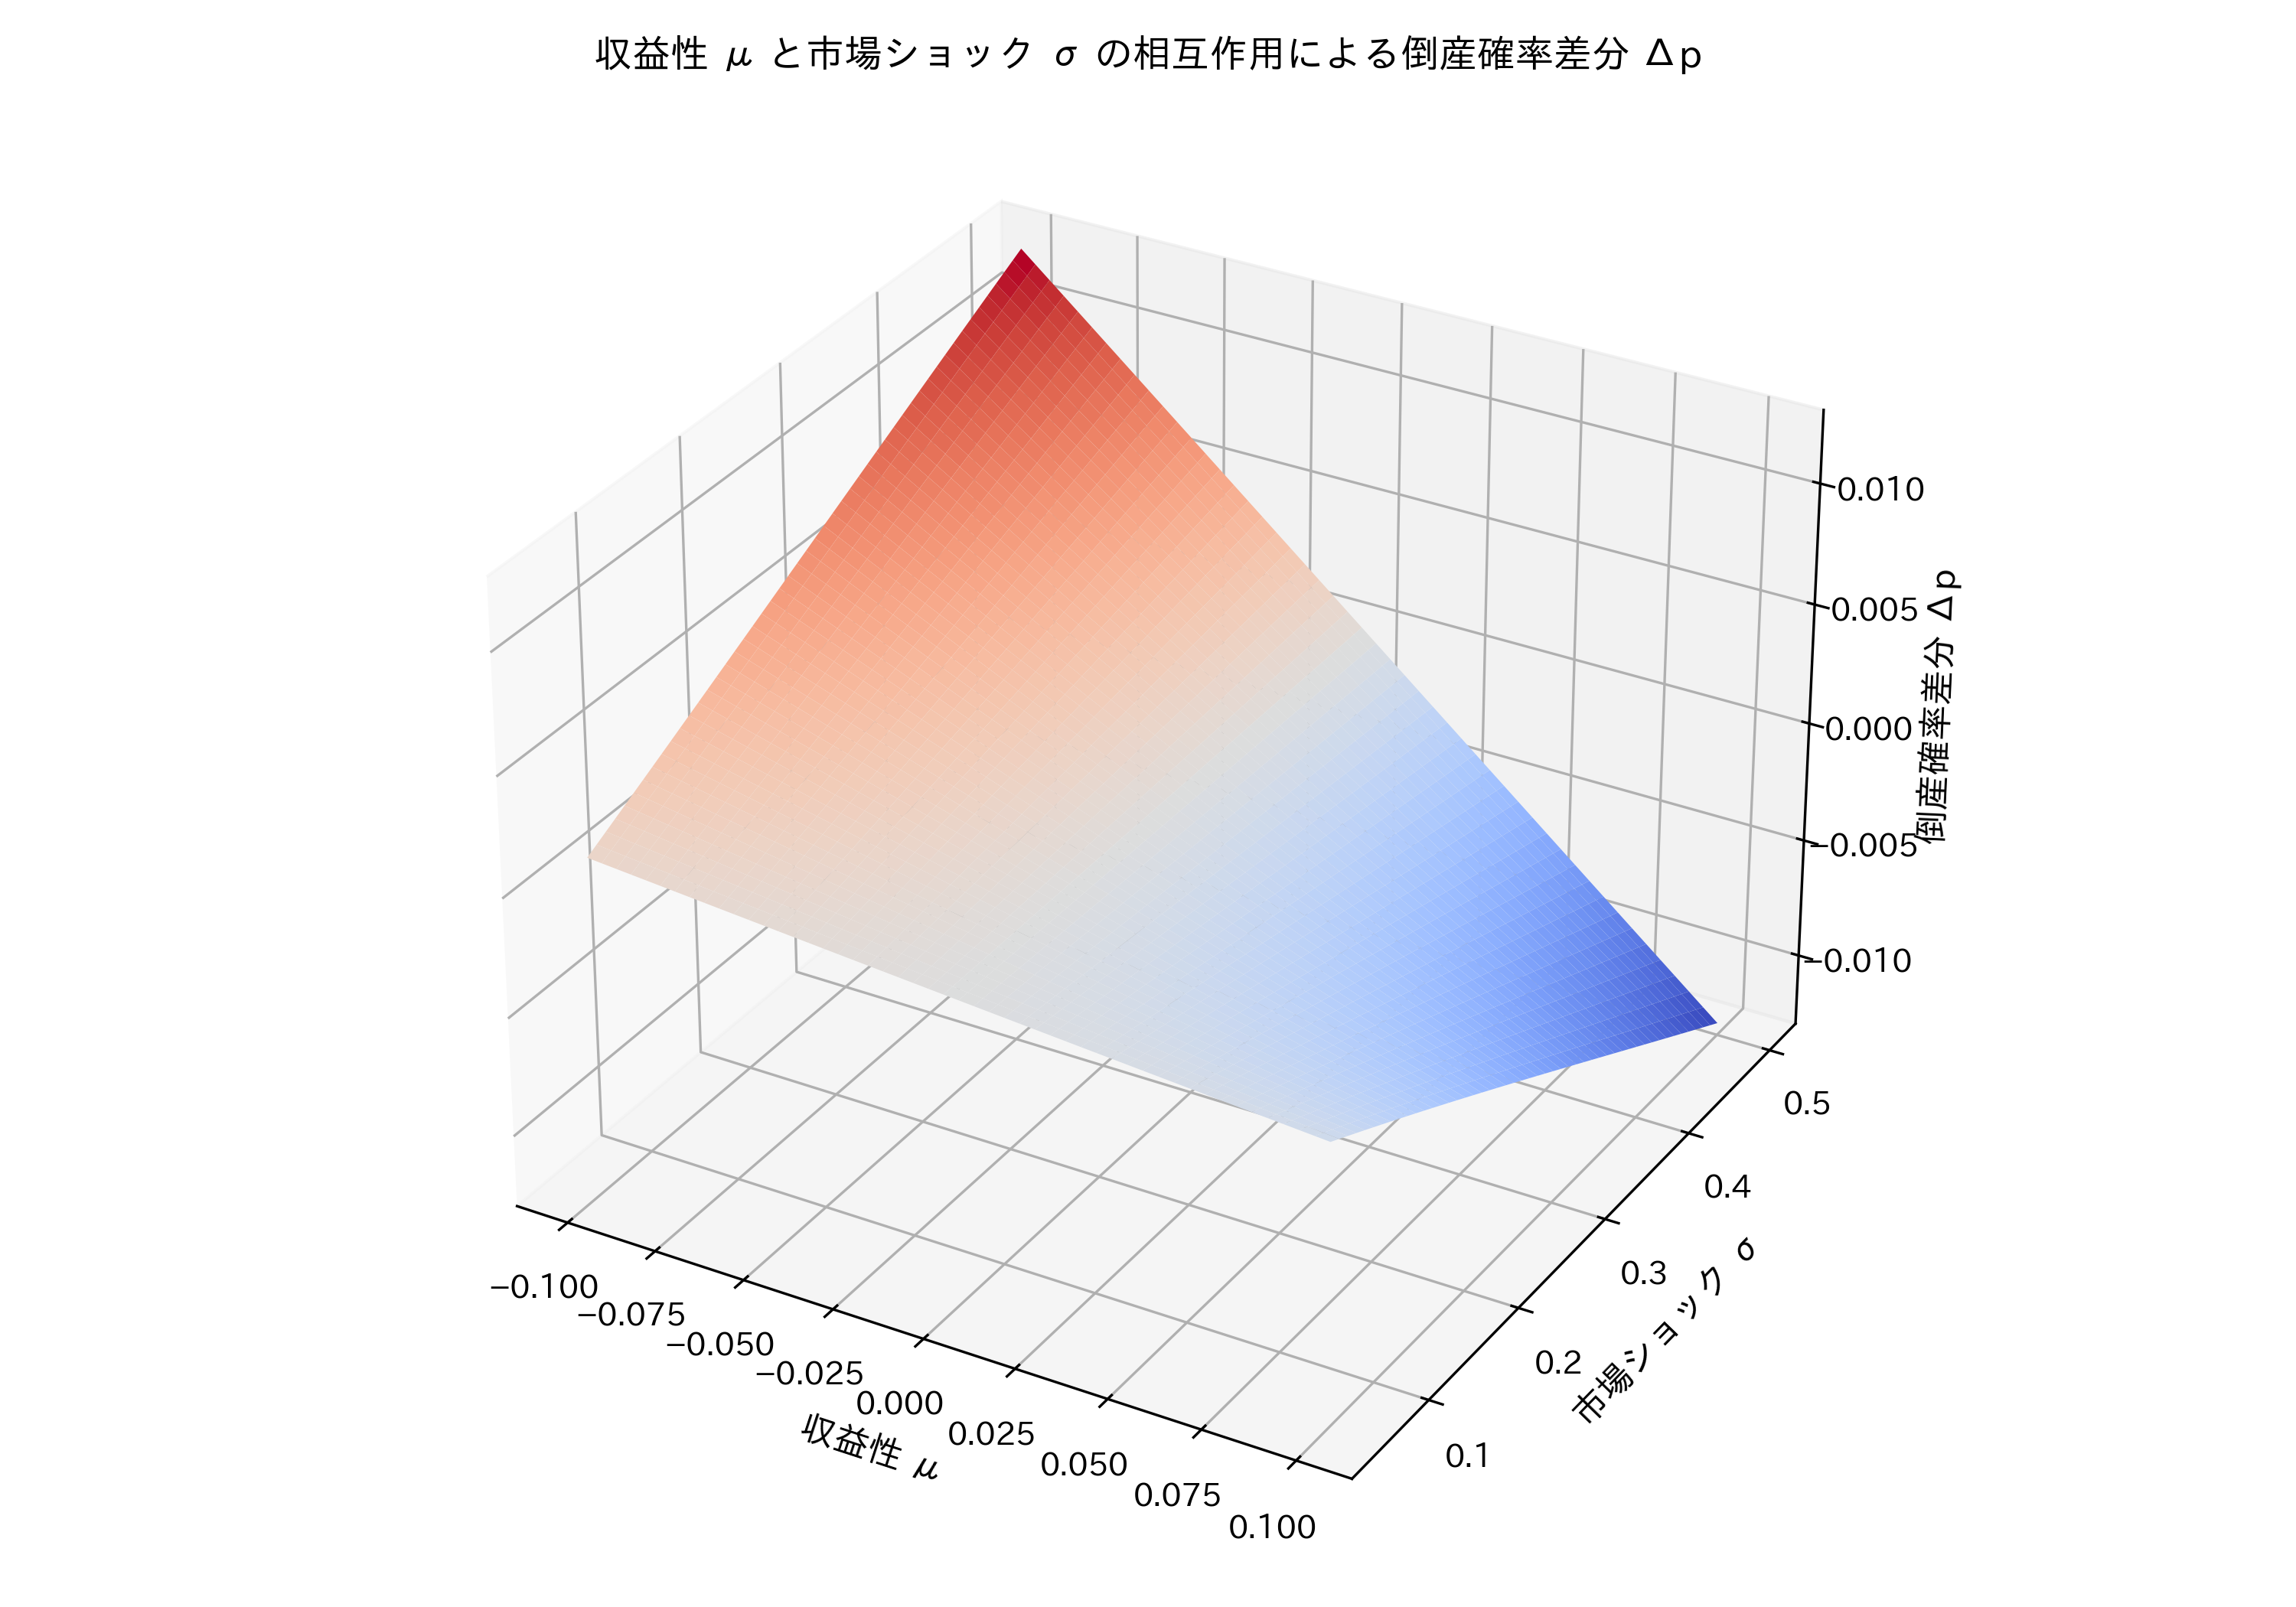
\includegraphics[width=0.80\linewidth]{figures/interaction_mu_sigma_surface.png}
    \caption{収益性 $\mu$ と市場ショック $\sigma$ の相互作用による倒産確率差分 $\Delta p$ の3Dサーフェス}
    \label{fig:interaction_mu_sigma_surface}
\end{figure}

図\ref{fig:interaction_mu_sigma_surface} は，収益性 $\mu$ と市場ショック $\sigma$ の相互作用項
$\gamma_{\mu\sigma}(\mu \cdot \sigma)$ が倒産確率に与える影響を可視化したものである。
相互作用を含む倒産確率 $p_{\mathrm{int}}$ と，相互作用を含まない倒産確率 $p_{\mathrm{base}}$ の差分



\[
\Delta p = p_{\mathrm{int}} - p_{\mathrm{base}}
\]



を3次元サーフェスとして描画している。
$\mu$ が低く $\sigma$ が高い領域で $\Delta p$ が大きくなることから，
収益性が低い企業ほど市場ショックの悪影響が増幅されることが確認できる。
一方，$\mu$ が高い領域では $\sigma$ の影響が緩和され，$\Delta p$ が小さくなる。
これは「収益性がショック耐性を高める」という理論モデルの含意と整合的である。

% ------------------------------------------------------------
% 図：S×D の相互作用
% ------------------------------------------------------------

\begin{figure}[H]
    \centering
    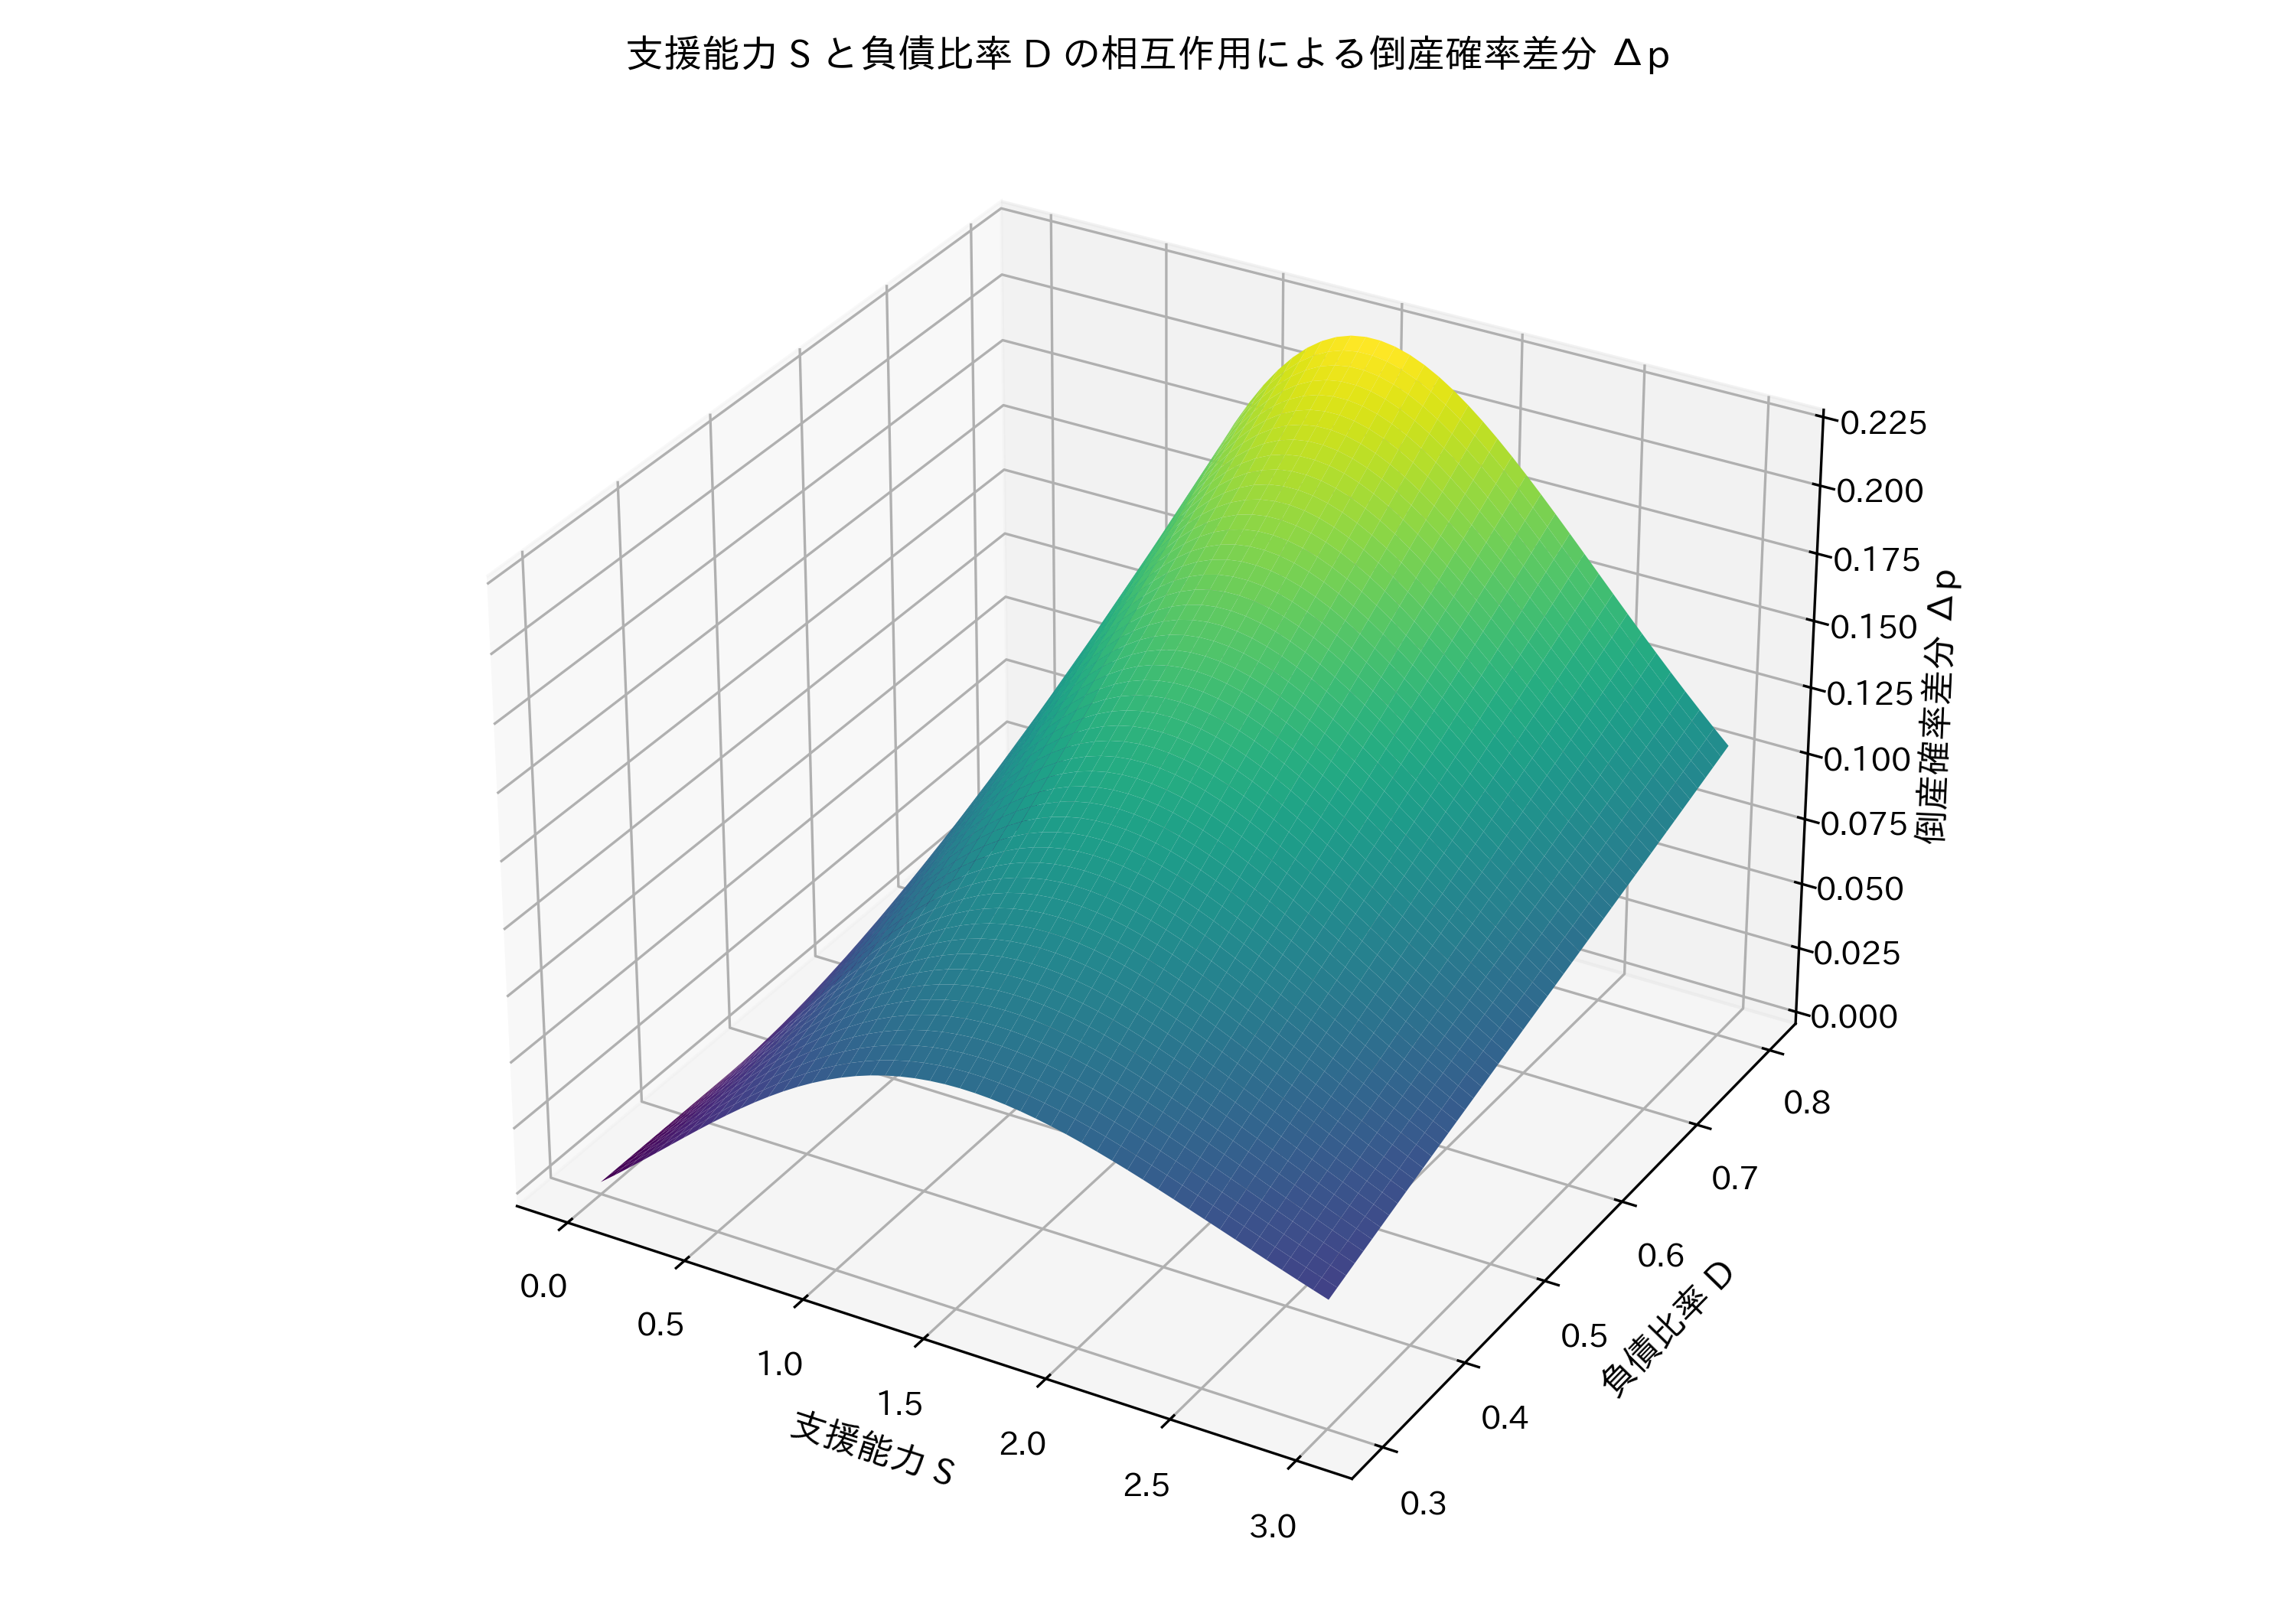
\includegraphics[width=0.80\linewidth]{figures/interaction_S_D_surface.png}
    \caption{支援能力 $S$ と負債比率 $D$ の相互作用による倒産確率差分 $\Delta p$ の3Dサーフェス}
    \label{fig:interaction_S_D_surface}
\end{figure}

図\ref{fig:interaction_S_D_surface} は，支援能力 $S$ と負債比率 $D$ の相互作用項
$\gamma_{SD}(S \cdot D)$ が倒産確率に与える影響を可視化したものである。
相互作用を含む倒産確率と含まない倒産確率の差分



\[
\Delta p = p_{\mathrm{int}} - p_{\mathrm{base}}
\]



を描画している。
$S$ が高い企業では，$D$ の上昇による倒産確率の悪化が大幅に緩和され，
$\Delta p$ が正の plateau（高原）として現れる。
一方，$S=0$ の企業では $D$ の悪影響がそのまま倒産確率に反映され，
$\Delta p$ はほぼゼロとなる。
これは「支援能力が負債過多の悪影響を吸収する」という理論的含意を
数値的に裏付けるものである。

\subsection*{相互関係シミュレーションの意義}

本節の相互関係シミュレーションは，以下の点で重要である。

\begin{itemize}
    \item 第4章の理論モデルで示した「相互作用の符号条件」を数値的に確認できる
    \item 第6.4節の可視化（ケース比較）で観察される非線形性の背景を説明できる
    \item 第8章の実証分析における交差項（$\mu \cdot \sigma$，$S \cdot D$）の導入を理論的に正当化する
\end{itemize}

特に，実証分析ではサンプル数の制約から交差項を 1〜2 個に限定する必要があるが，
本節のシミュレーションにより，
\textbf{どの交差項が倒産確率に最も強く作用するかを事前に把握できる}
点に意義がある。

以上より，本節は理論モデルと実証分析を橋渡しする役割を果たし，
倒産リスクの構造が単一要因ではなく複数要因の相互作用によって決定されることを
数理的に示すものである。



\section{可視化とケース比較}
% ------------------------------------------------------------
% 7.7 可視化とケース比較
% 
% ・ケース設定と3D可視化を統合し、Z_lin の構造を視覚的に確認する
% ・S と D の違いが倒産確率の地形にどう現れるかを体系的に整理する
% ・第7章の実証分析につながる橋渡しの役割を持つ
% ------------------------------------------------------------

本節では，前節で定義した潜在倒産距離


\[
Z_{\text{lin}} = \mu - \sigma + S - D
\]


およびロジット写像


\[
p = \frac{1}{1 + \exp(-Z_{\text{lin}})}
\]


を用いて，新電力企業の倒産確率がどのような地形を描くのかを可視化する。
特に，支援能力 $S$ と負債比率 $D$ が倒産確率の基準水準をどのように規定するのかを，
代表的なケース設定と 3D サーフェスプロットを通じて比較する。

% ============================================================
\subsection{ケース設定}
% ------------------------------------------------------------
% ・企業の典型的な財務状態を6ケースに分類
% ・S と D の組合せが Z_lin の基準水準をどう規定するかを示す
% ・第7章の実証分析で用いる財務プロファイルの基礎分類
% ------------------------------------------------------------

本研究では，新電力企業の典型的な財務状態と資本構造を踏まえ，
倒産リスクの構造的特徴を把握するために，以下の 6 ケースを設定する。
これらは，負債比率 $D$ と支援能力 $S$ の代表的な組合せを体系的に網羅したものであり，
新電力企業の多様な財務プロファイルを抽象化した分類である。

\begin{itemize}
    \item ケースA：$D=0.3,\ S=0$（独立系・財務健全）
    \item ケースB：$D=0.3,\ S=3$（大手系・財務健全）
    \item ケースC：$D=0.8,\ S=0$（独立系・負債過多）
    \item ケースD：$D=0.8,\ S=3$（大手系・負債過多）
    \item ケースE：$D=0.5,\ S=1$（地域新電力）
    \item ケースF：$D=0.5,\ S=2$（商社系）
\end{itemize}

これらのケースは，$Z_{\text{lin}}$ の構造において，
支援能力 $S$ が倒産確率の「底上げ」を行い，
負債比率 $D$ がその逆方向に作用するという基本的な力学を比較するための基盤となる。

% ============================================================
\subsection{3D サーフェスプロットによる可視化}
% ------------------------------------------------------------
% ・μ と σ を連続的に動かし，p の3D地形を描画する
% ・S と D の違いが地形の位置と急峻性にどう現れるかを確認
% ・理論モデルの符号条件が視覚的に再現されることを示す
% ------------------------------------------------------------

本節では，各ケースについて倒産確率 $p$ の 3 次元サーフェスプロットを作成し，
$Z_{\text{lin}}$ の符号条件がどのように地形として現れるかを確認する。
以下では，ケースA〜Fの順に図を示し，それぞれの特徴を簡潔に整理する。

% ---------- ケースA ----------
\subsubsection*{ケースA：$D=0.3,\ S=0$（独立系・財務健全）}

\begin{figure}[H]
    \centering
    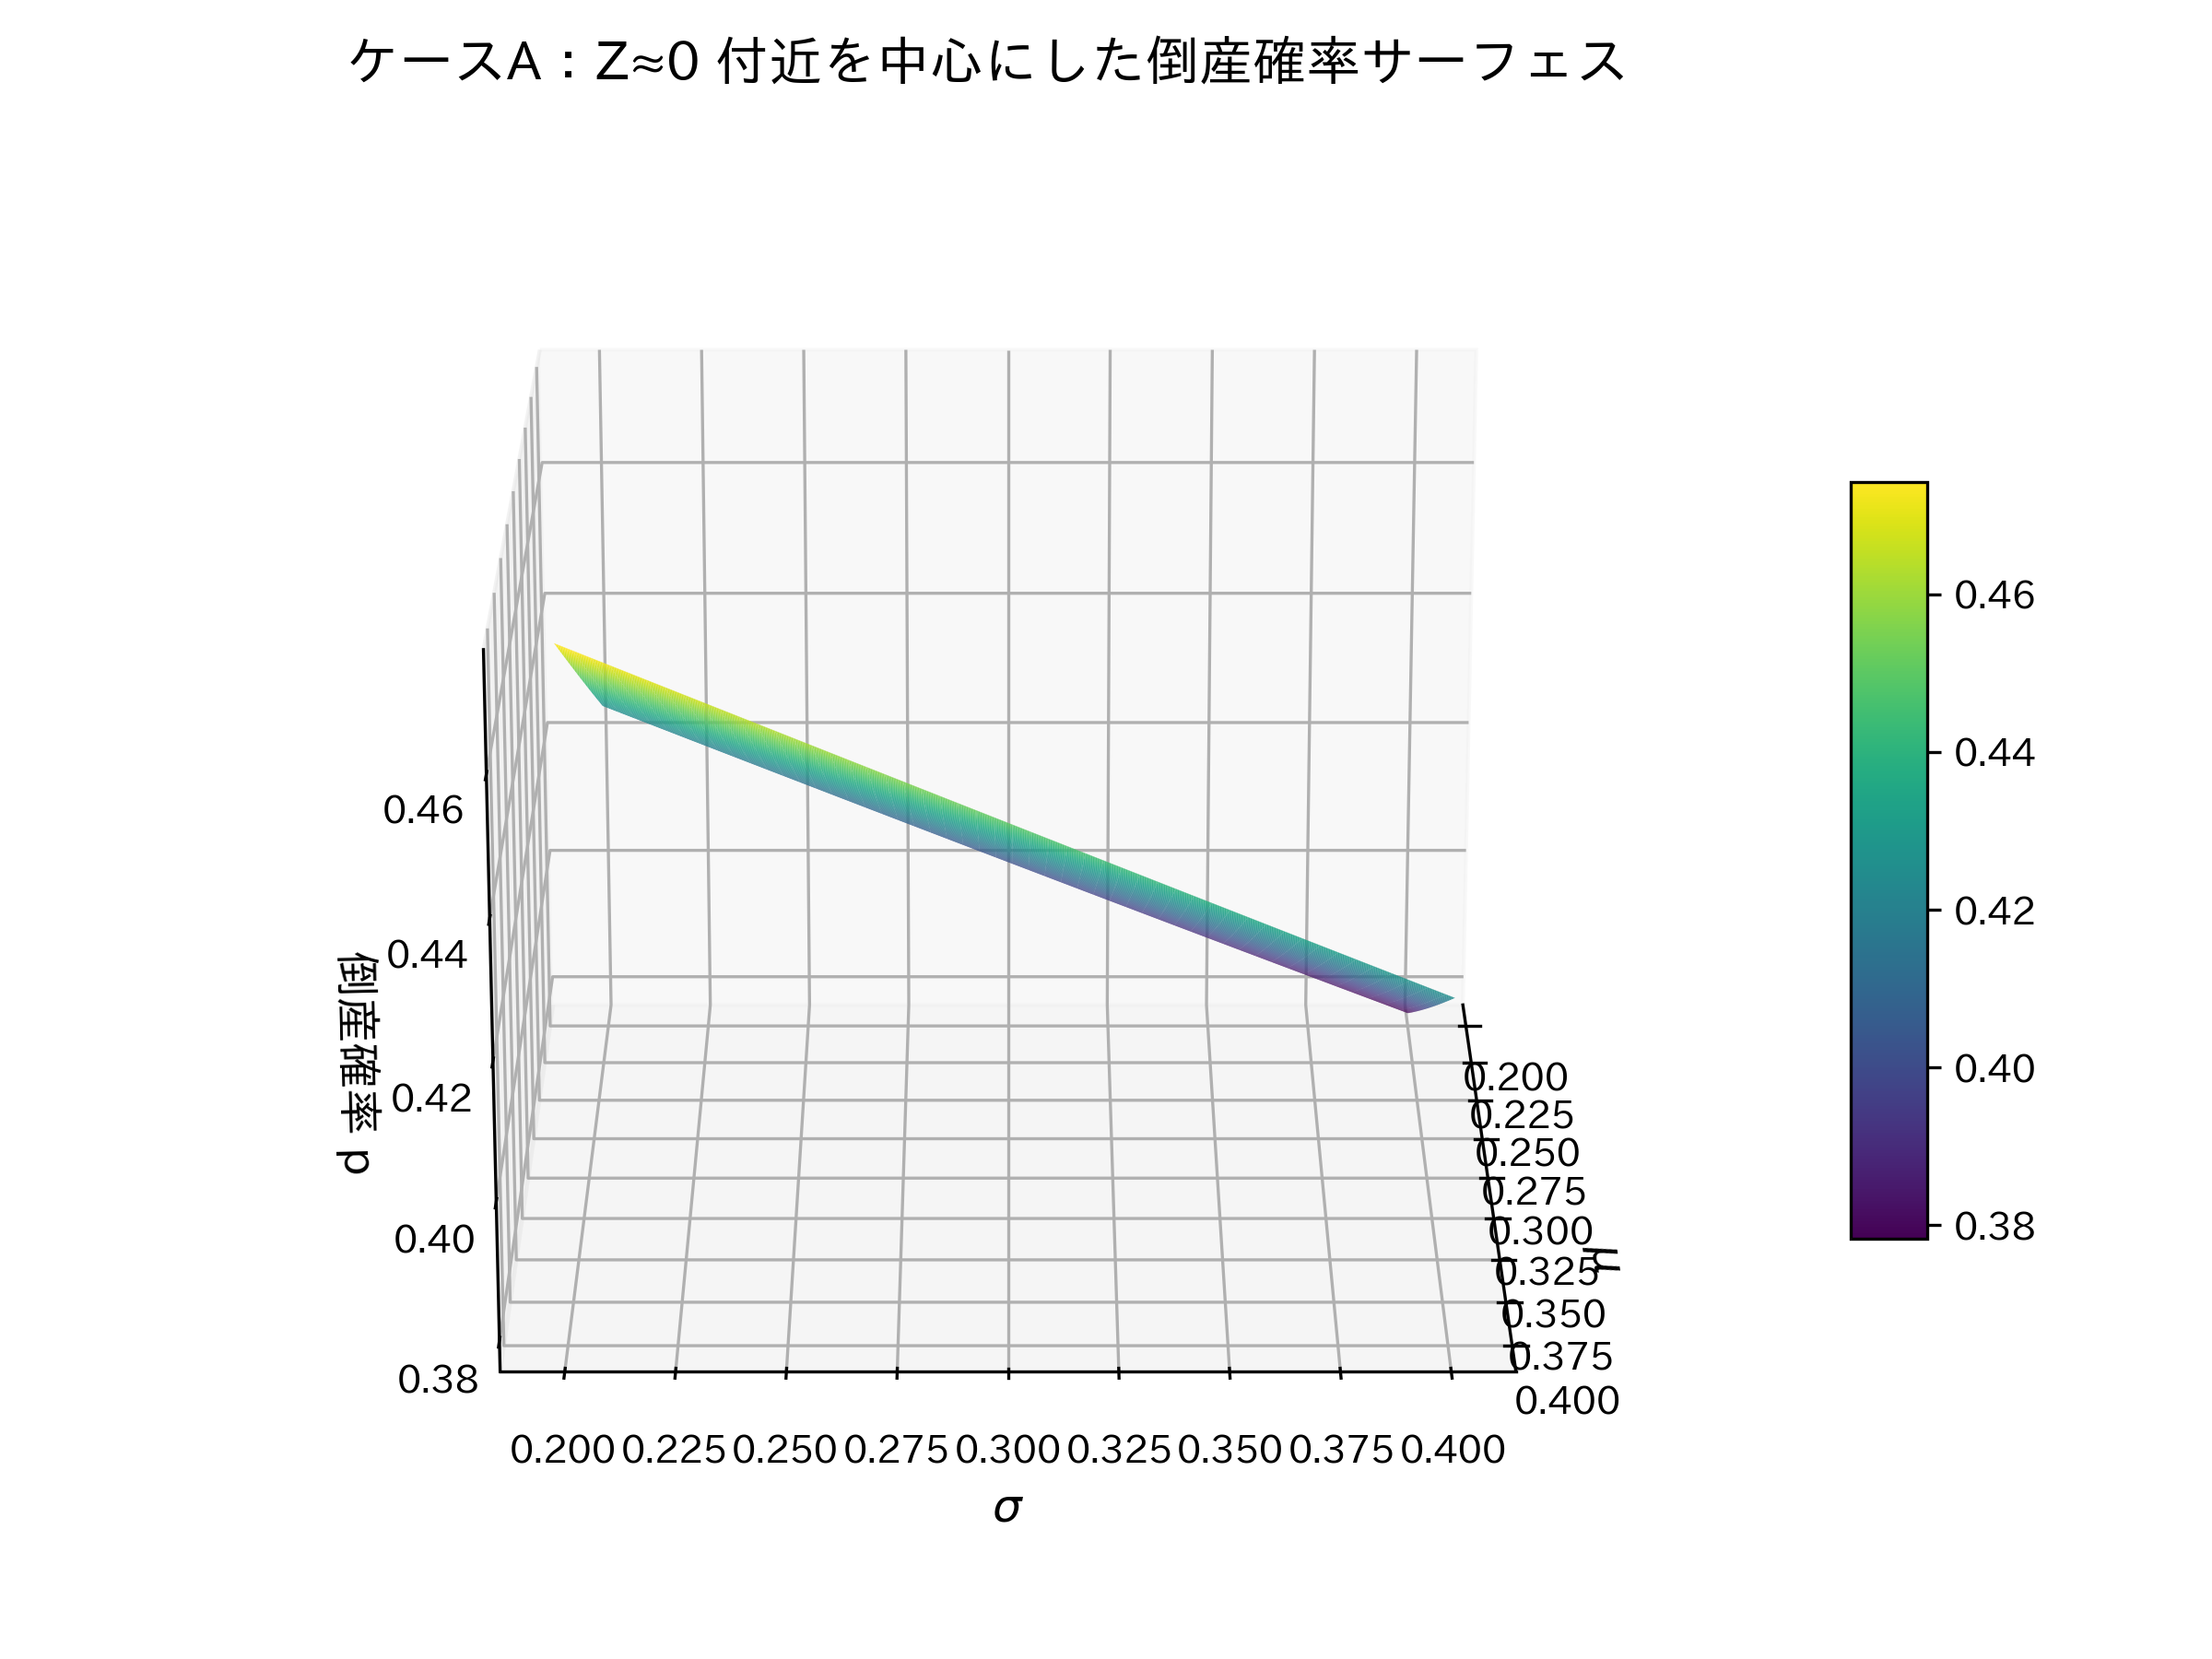
\includegraphics[width=0.75\linewidth]{figures/surface_caseA_centered.png}
    \caption{ケースAにおける倒産確率の3Dサーフェスプロット（Z≈0付近を中心）}
    \label{fig:surface_caseA_centered}
\end{figure}

ケースAでは，支援能力がなく負債比率も低いため，
倒産確率の基準水準は比較的低い。
Z≈0 付近を中心に描画することで，
$\sigma$ の上昇に対する急峻な立ち上がりがより明確に示され，
外生ショックへの脆弱性が視覚的に強調される。


% ---------- ケースB ----------
\subsubsection*{ケースB：$D=0.3,\ S=3$（大手系・財務健全）}

\begin{figure}[H]
    \centering
    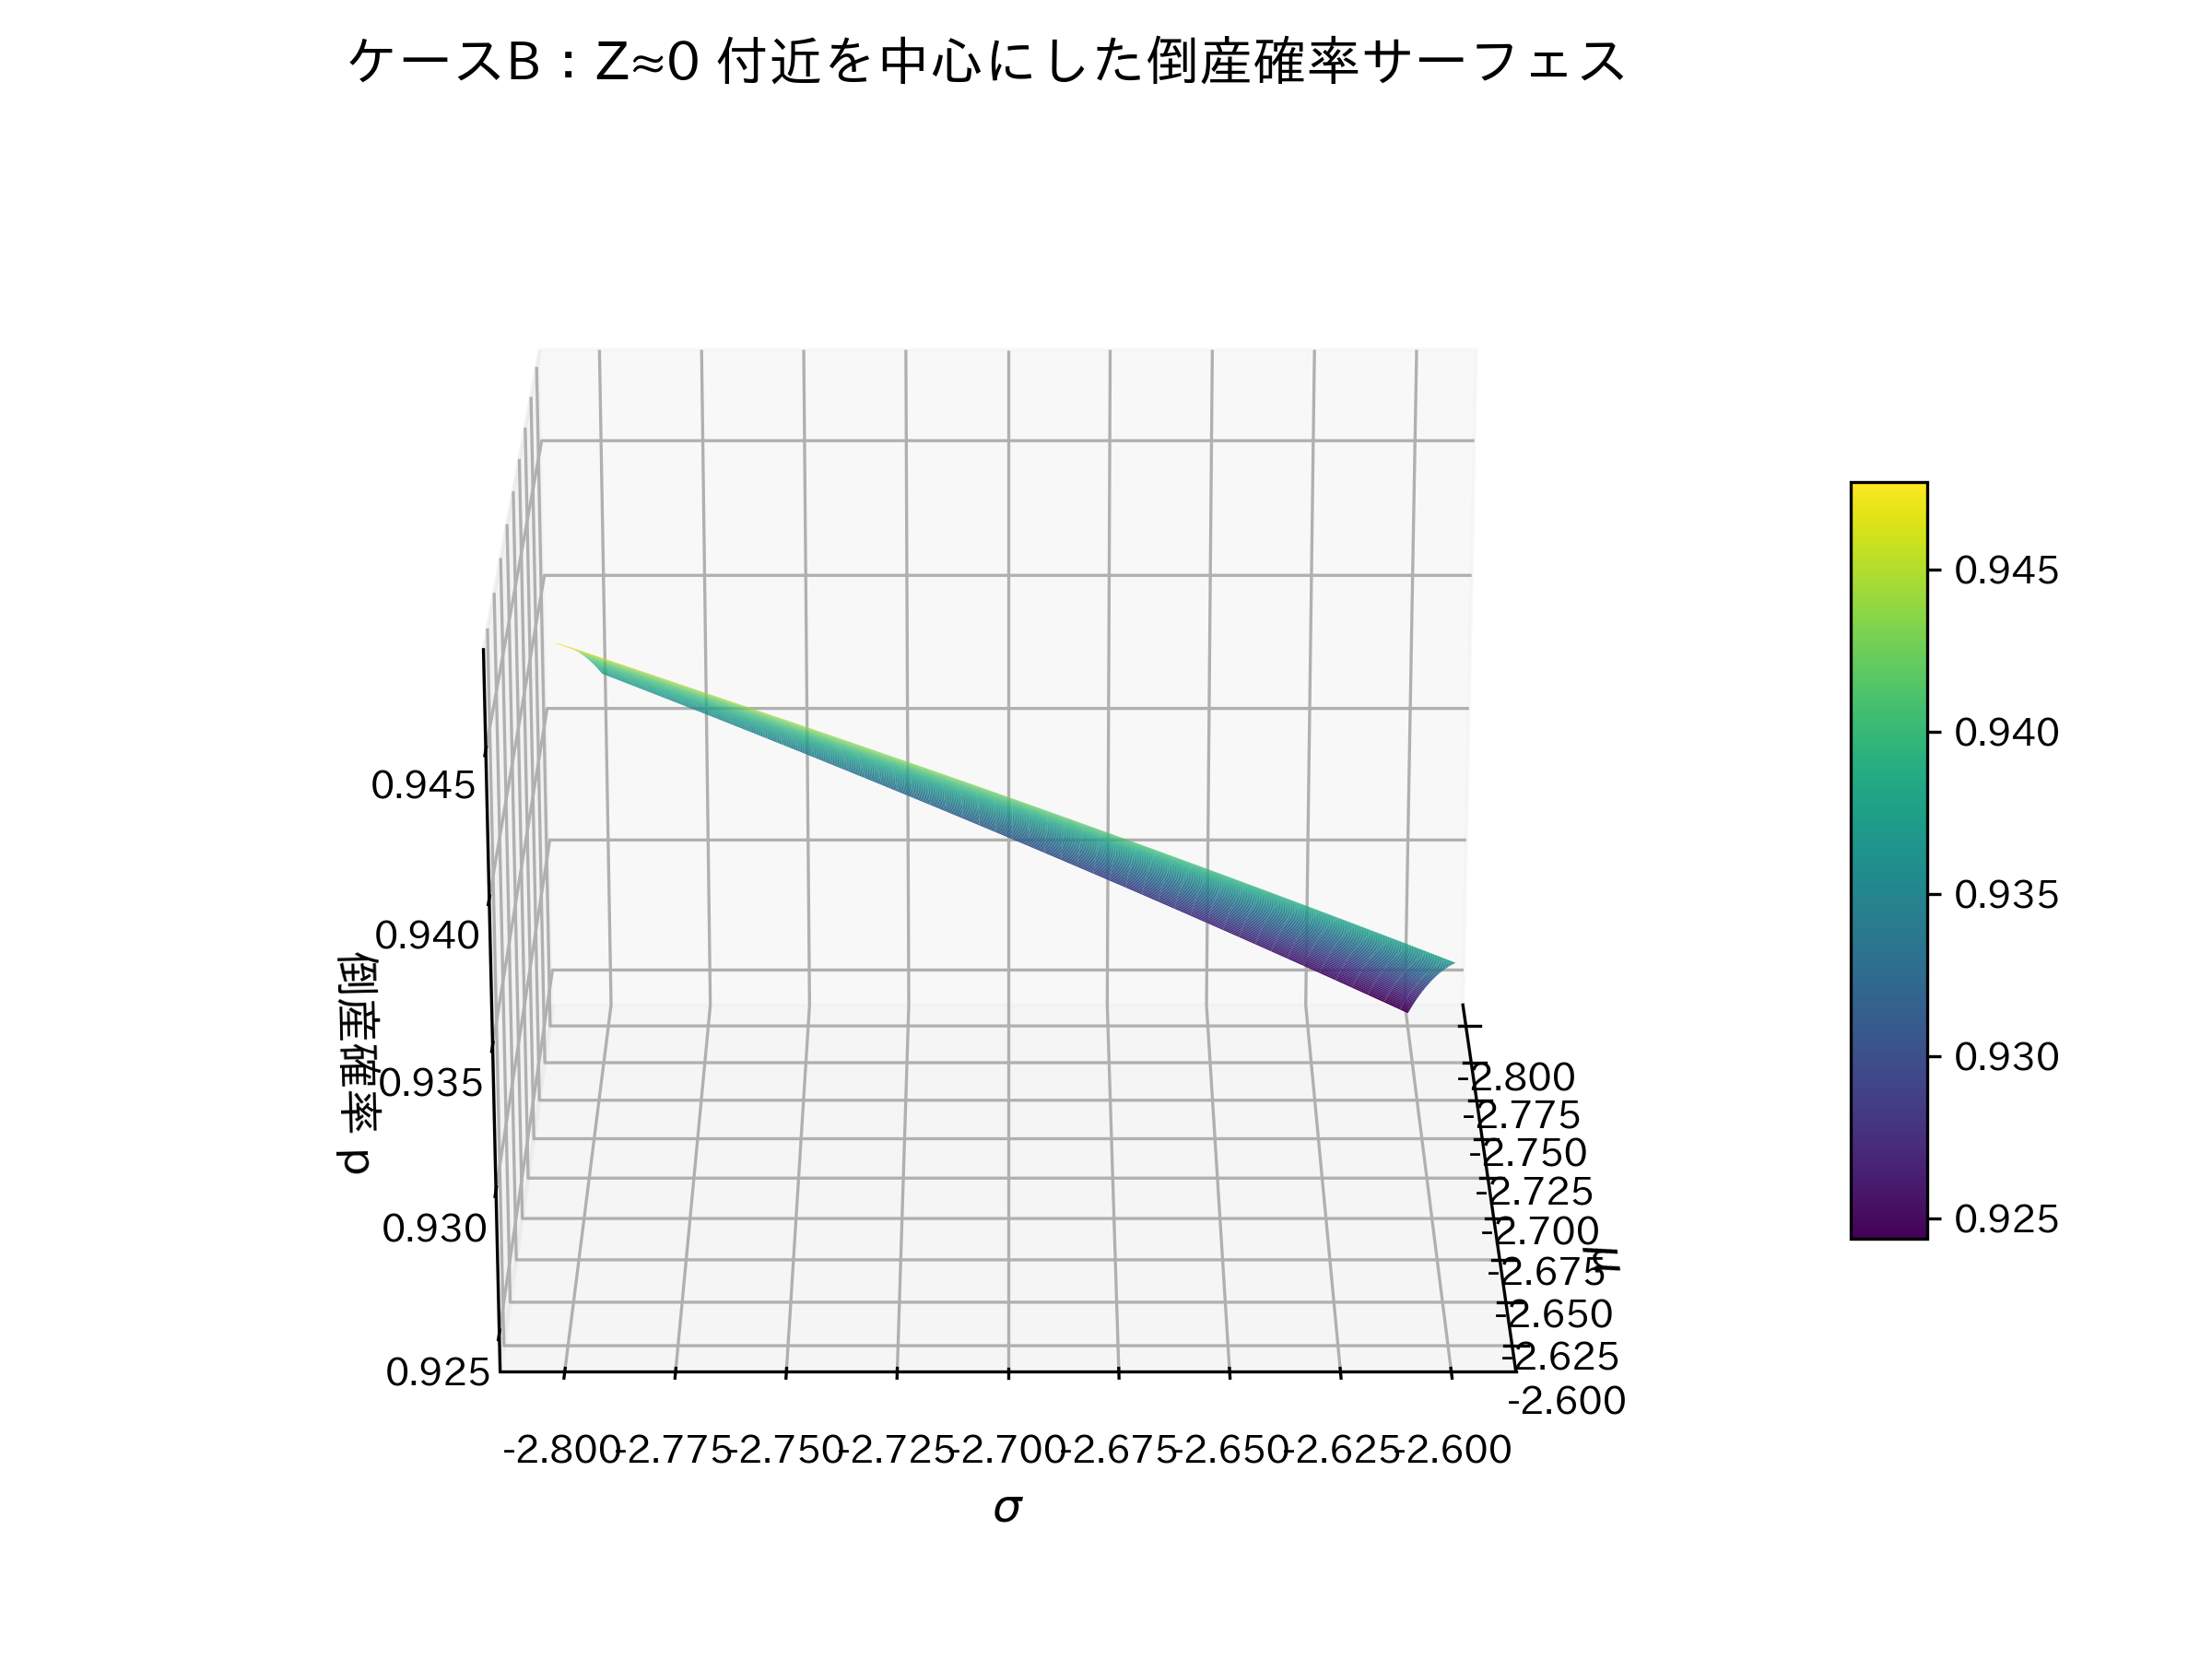
\includegraphics[width=0.75\linewidth]{figures/surface_caseB_centered.png}
    \caption{ケースBにおける倒産確率の3Dサーフェスプロット（Z≈0付近を中心）}
    \label{fig:surface_caseB_centered}
\end{figure}

ケースBでは，$S=3$ の強い支援能力により，
倒産確率の地形全体が大きく右方へシフトする。
Z≈0 を中心に描くことで，
支援能力が倒産境界線をどれほど押し下げるかが明確に可視化される。


% ---------- ケースC ----------
\subsubsection*{ケースC：$D=0.8,\ S=0$（独立系・負債過多）}

\begin{figure}[H]
    \centering
    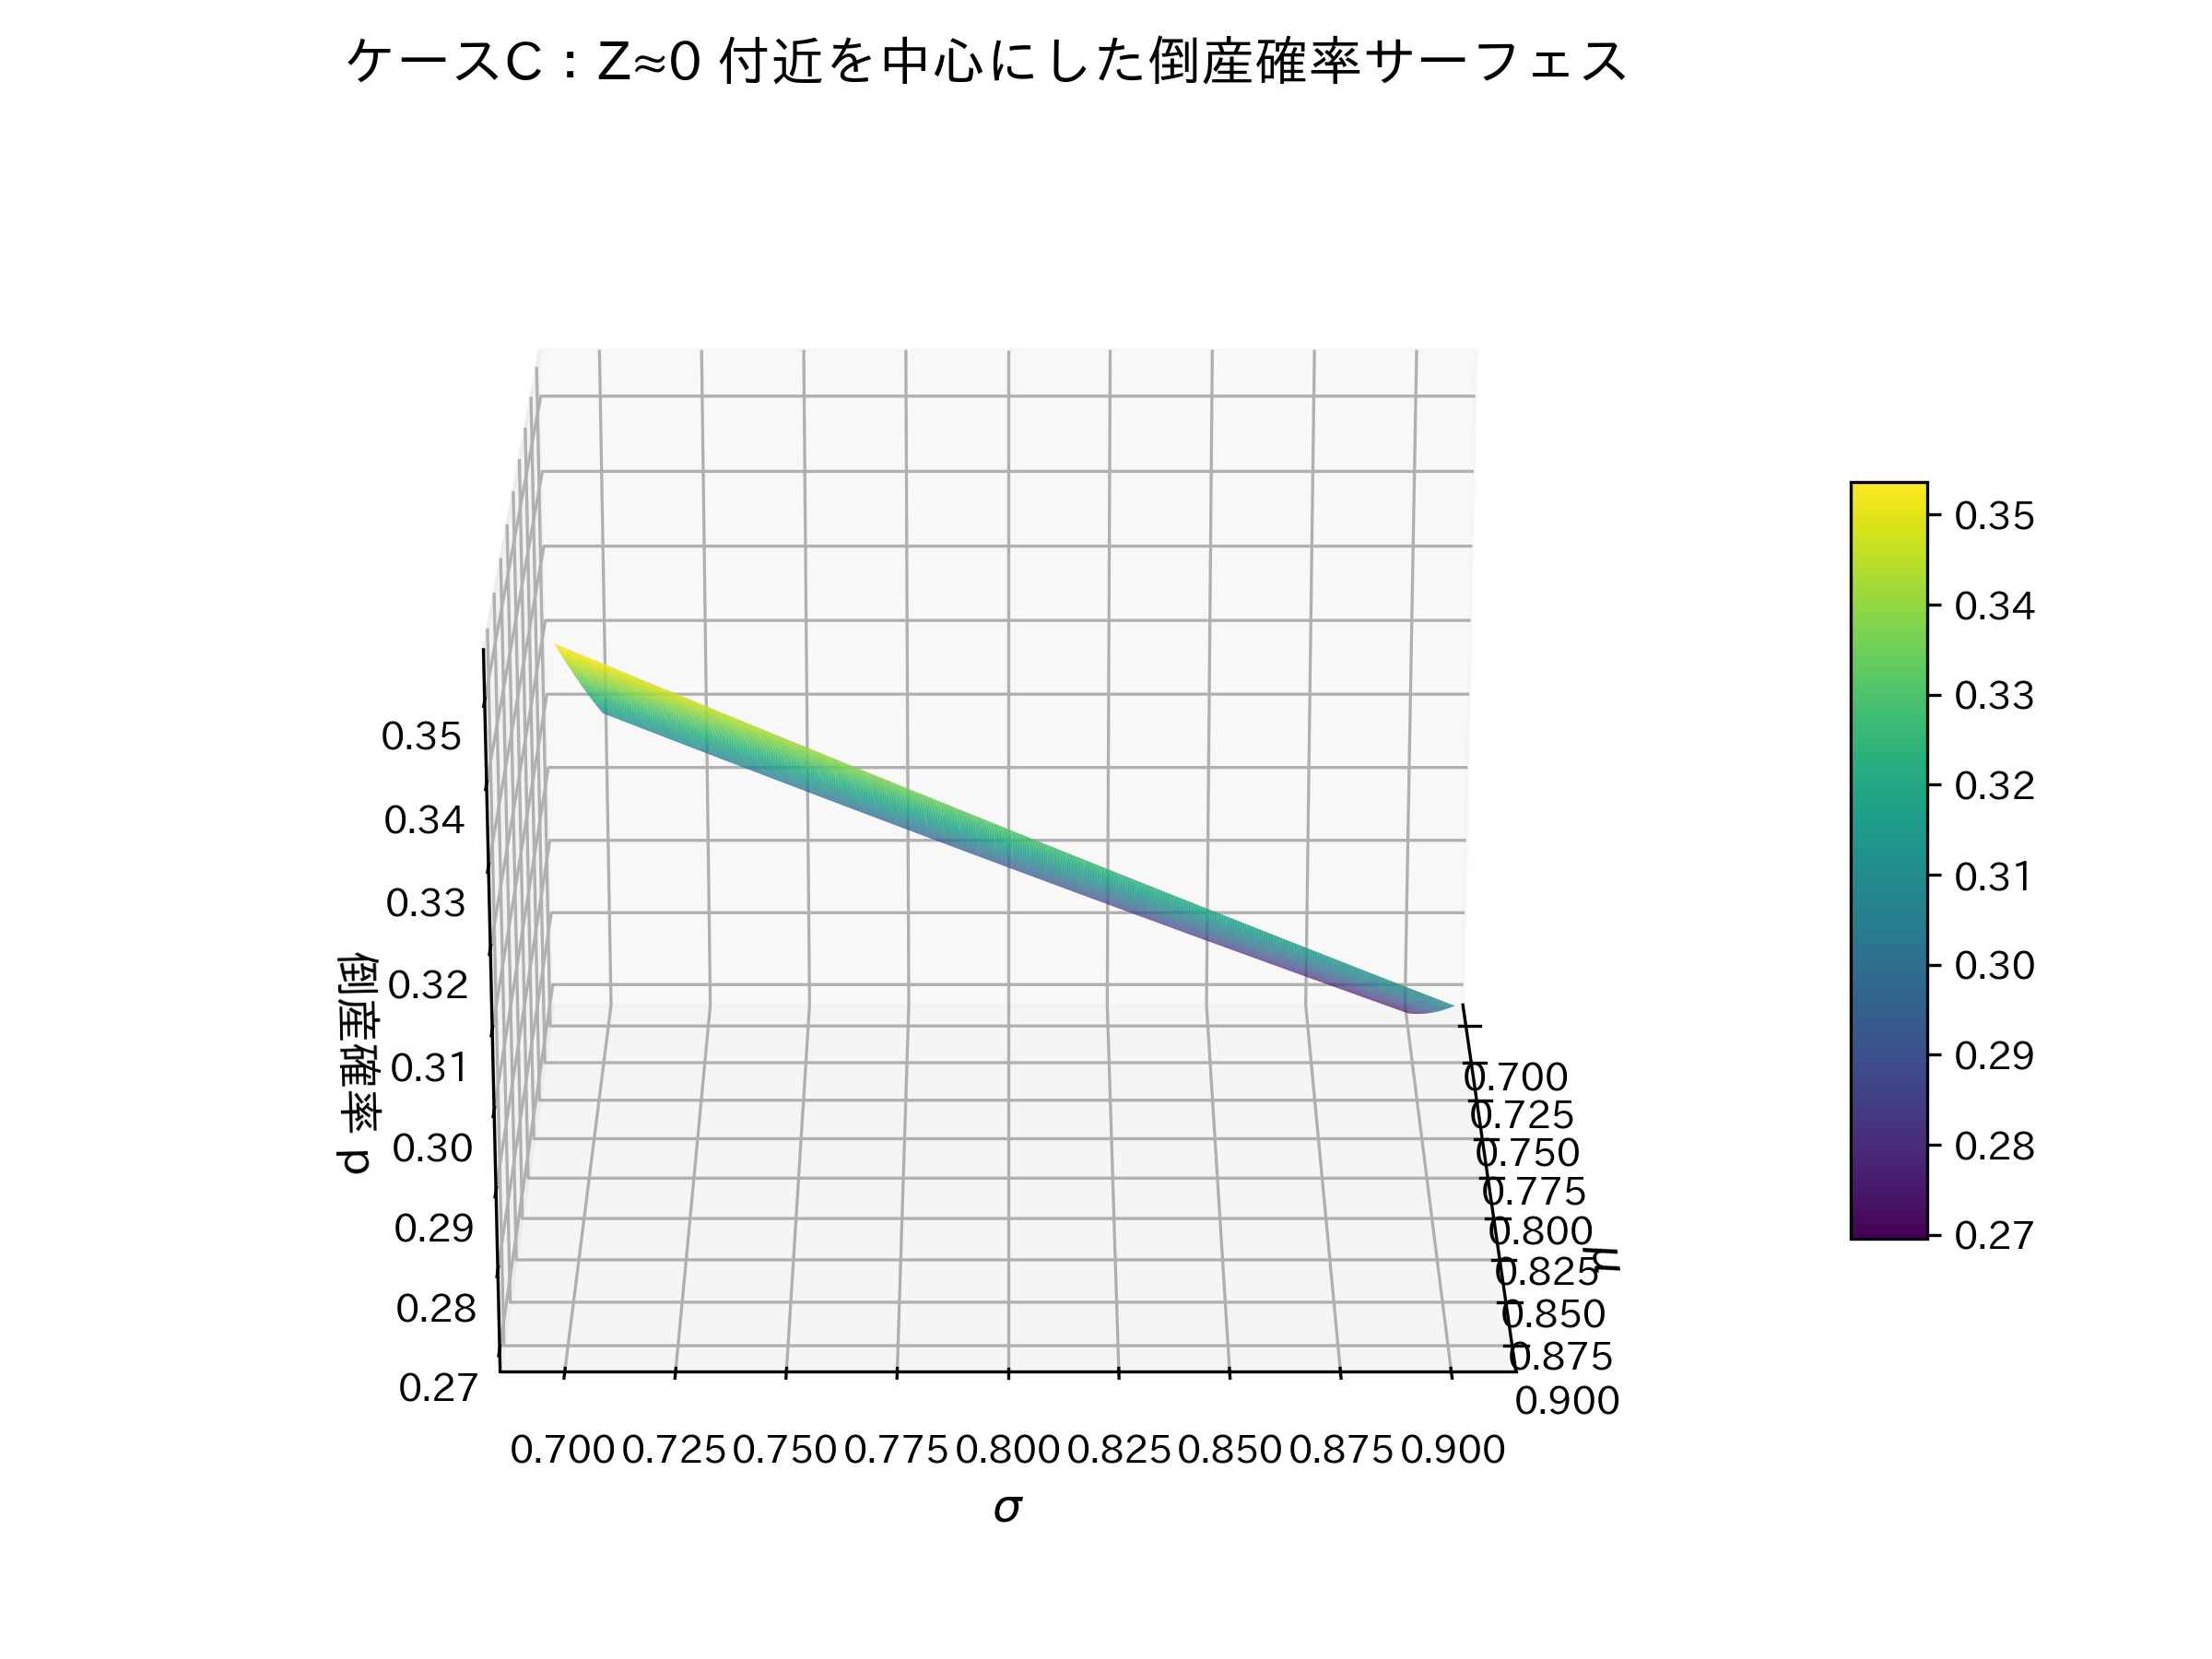
\includegraphics[width=0.75\linewidth]{figures/surface_caseC_centered.png}
    \caption{ケースCにおける倒産確率の3Dサーフェスプロット（Z≈0付近を中心）}
    \label{fig:surface_caseC_centered}
\end{figure}

ケースCでは，負債比率が高いため，
倒産確率の基準水準が大きく左方に位置し，倒産しやすい構造となる。
Z≈0 を中心に描くことで，
$\sigma$ の上昇に対する反応が極めて急峻であることが強調され，
高ボラティリティ環境での脆弱性が顕著に示される。


% ---------- ケースD ----------
\subsubsection*{ケースD：$D=0.8,\ S=3$（大手系・負債過多）}

\begin{figure}[H]
    \centering
    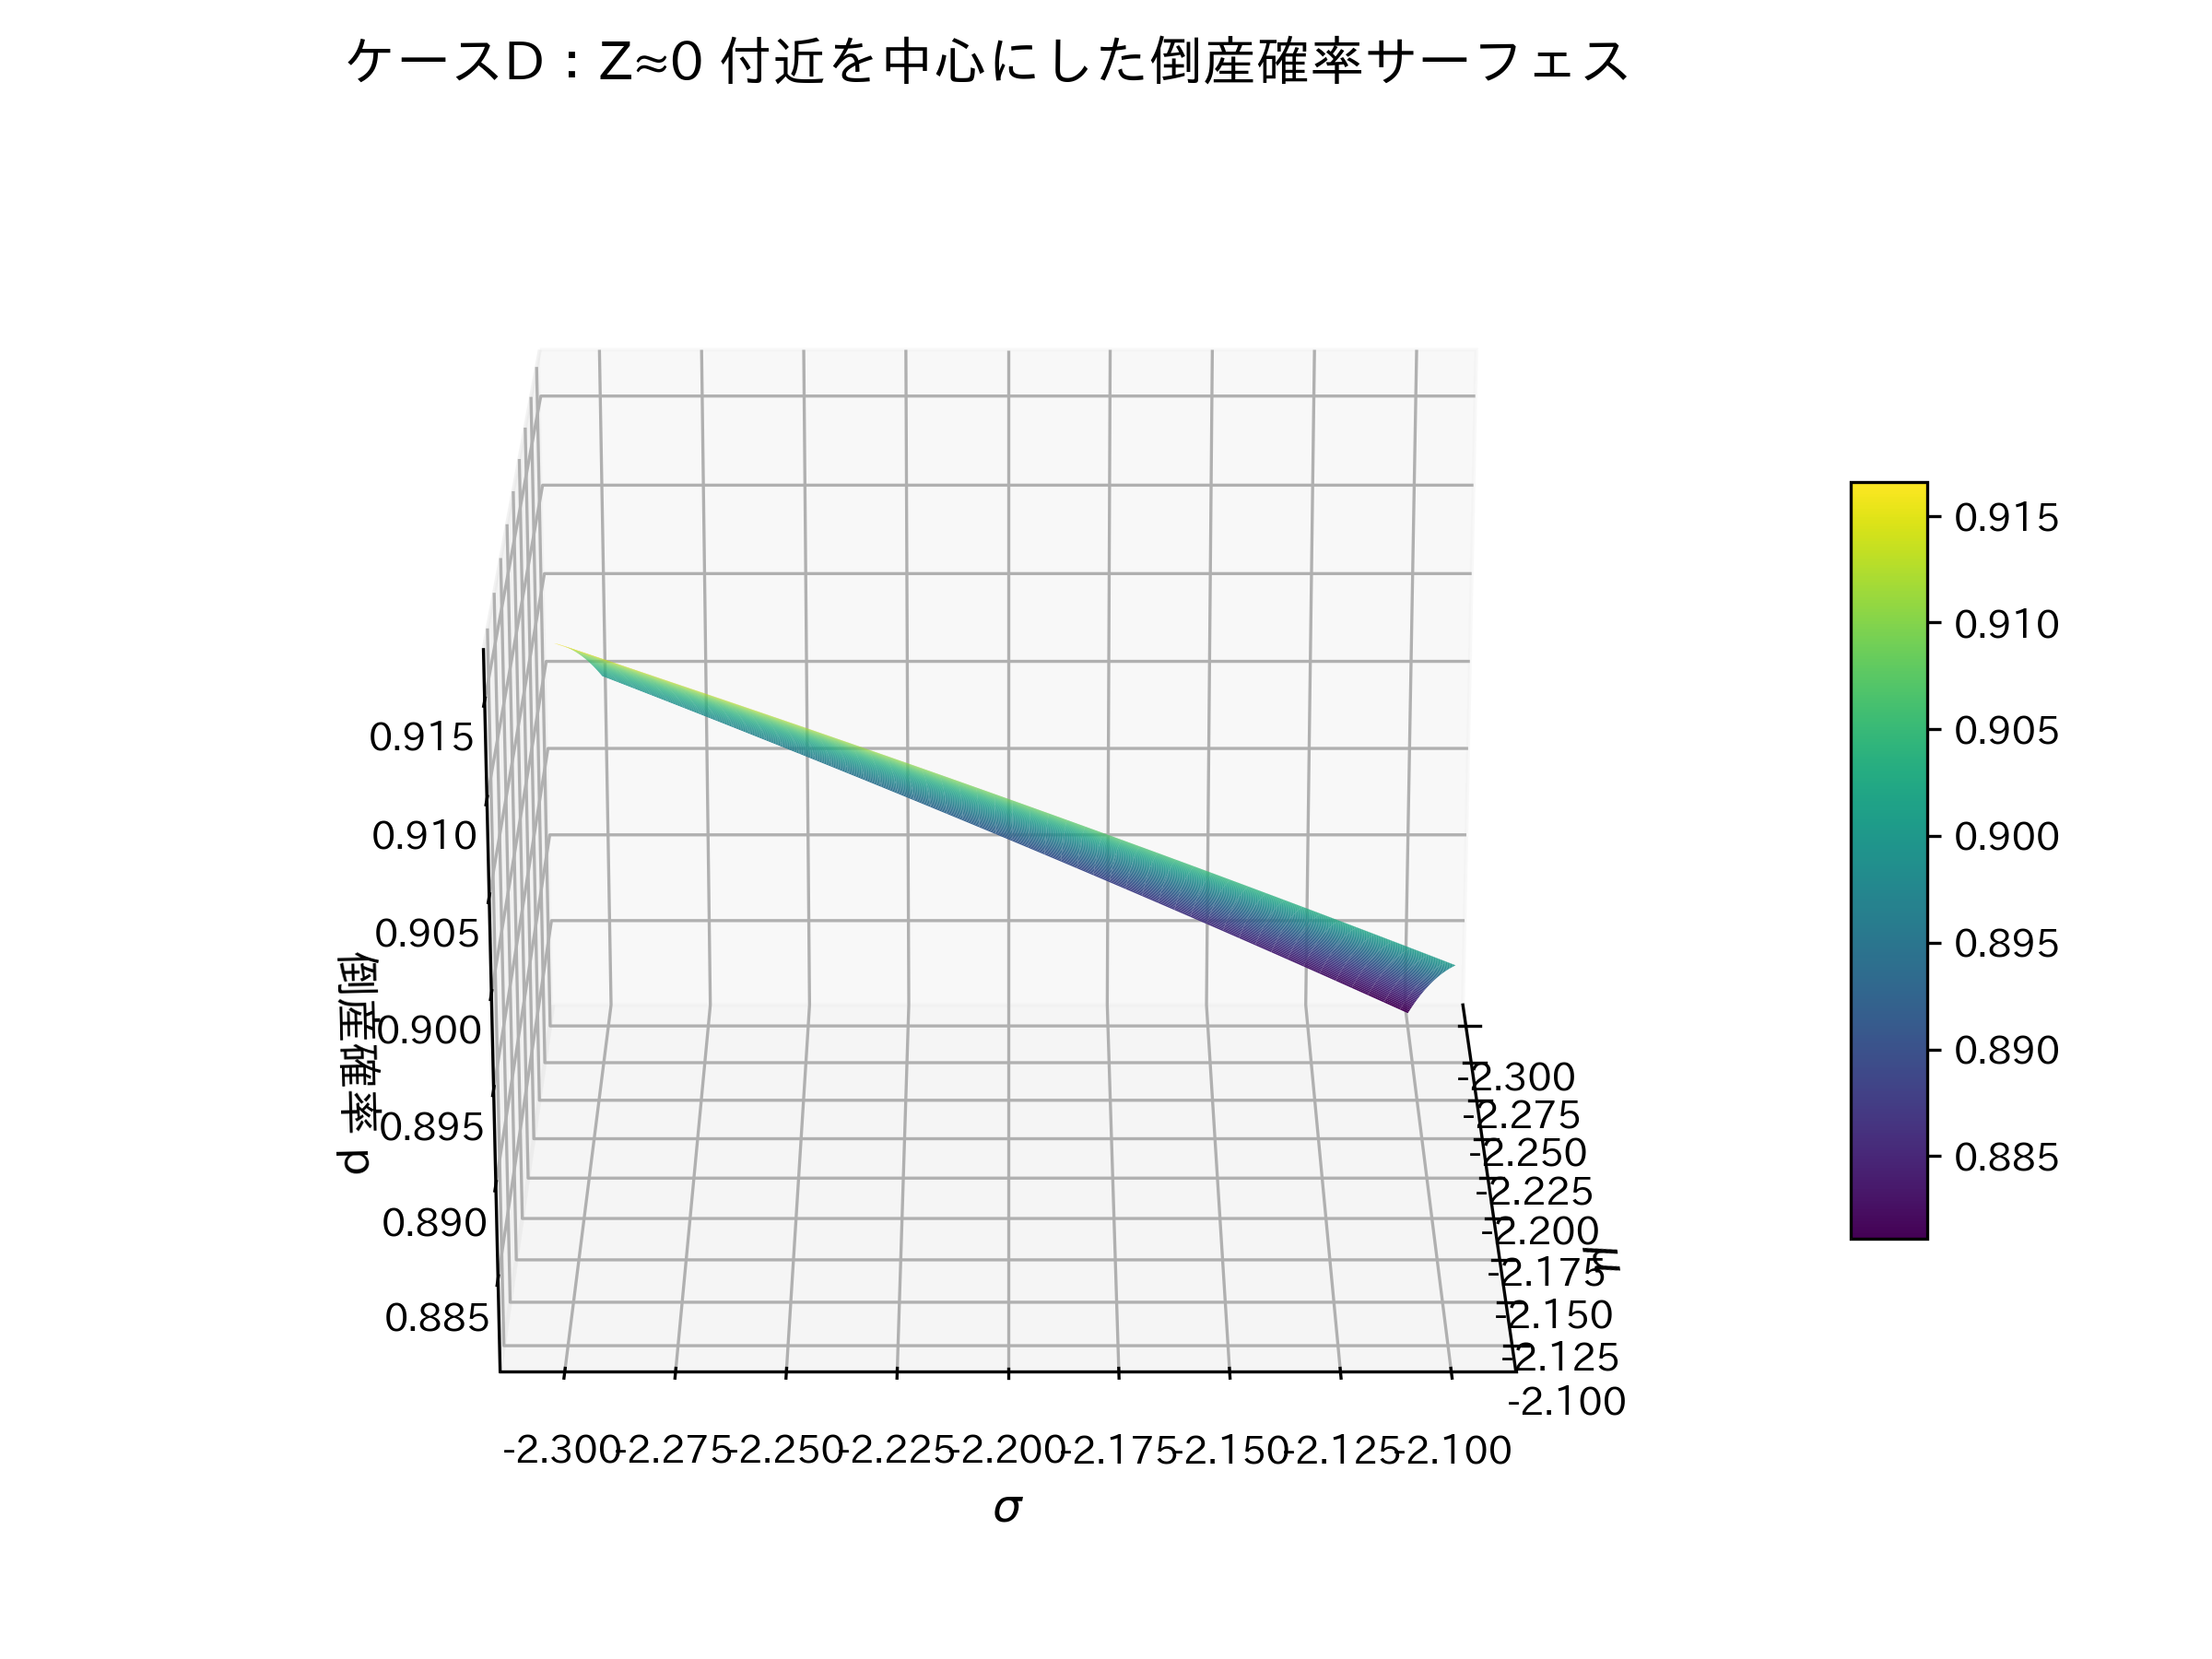
\includegraphics[width=0.75\linewidth]{figures/surface_caseD_centered.png}
    \caption{ケースDにおける倒産確率の3Dサーフェスプロット（Z≈0付近を中心）}
    \label{fig:surface_caseD_centered}
\end{figure}

ケースDでは，負債比率は高いものの，
強い支援能力により倒産確率の地形が右方へ押し戻される。
Z≈0 を中心に描くことで，
「高負債 × 強支援」という構造が倒産境界線の位置にどのように反映されるかが明確となる。
ただし $\sigma$ の影響は依然として大きく，
高ボラティリティ環境でのリスクは残存する。


% ---------- ケースE ----------
\subsubsection*{ケースE：$D=0.5,\ S=1$（地域新電力）}

\begin{figure}[H]
    \centering
    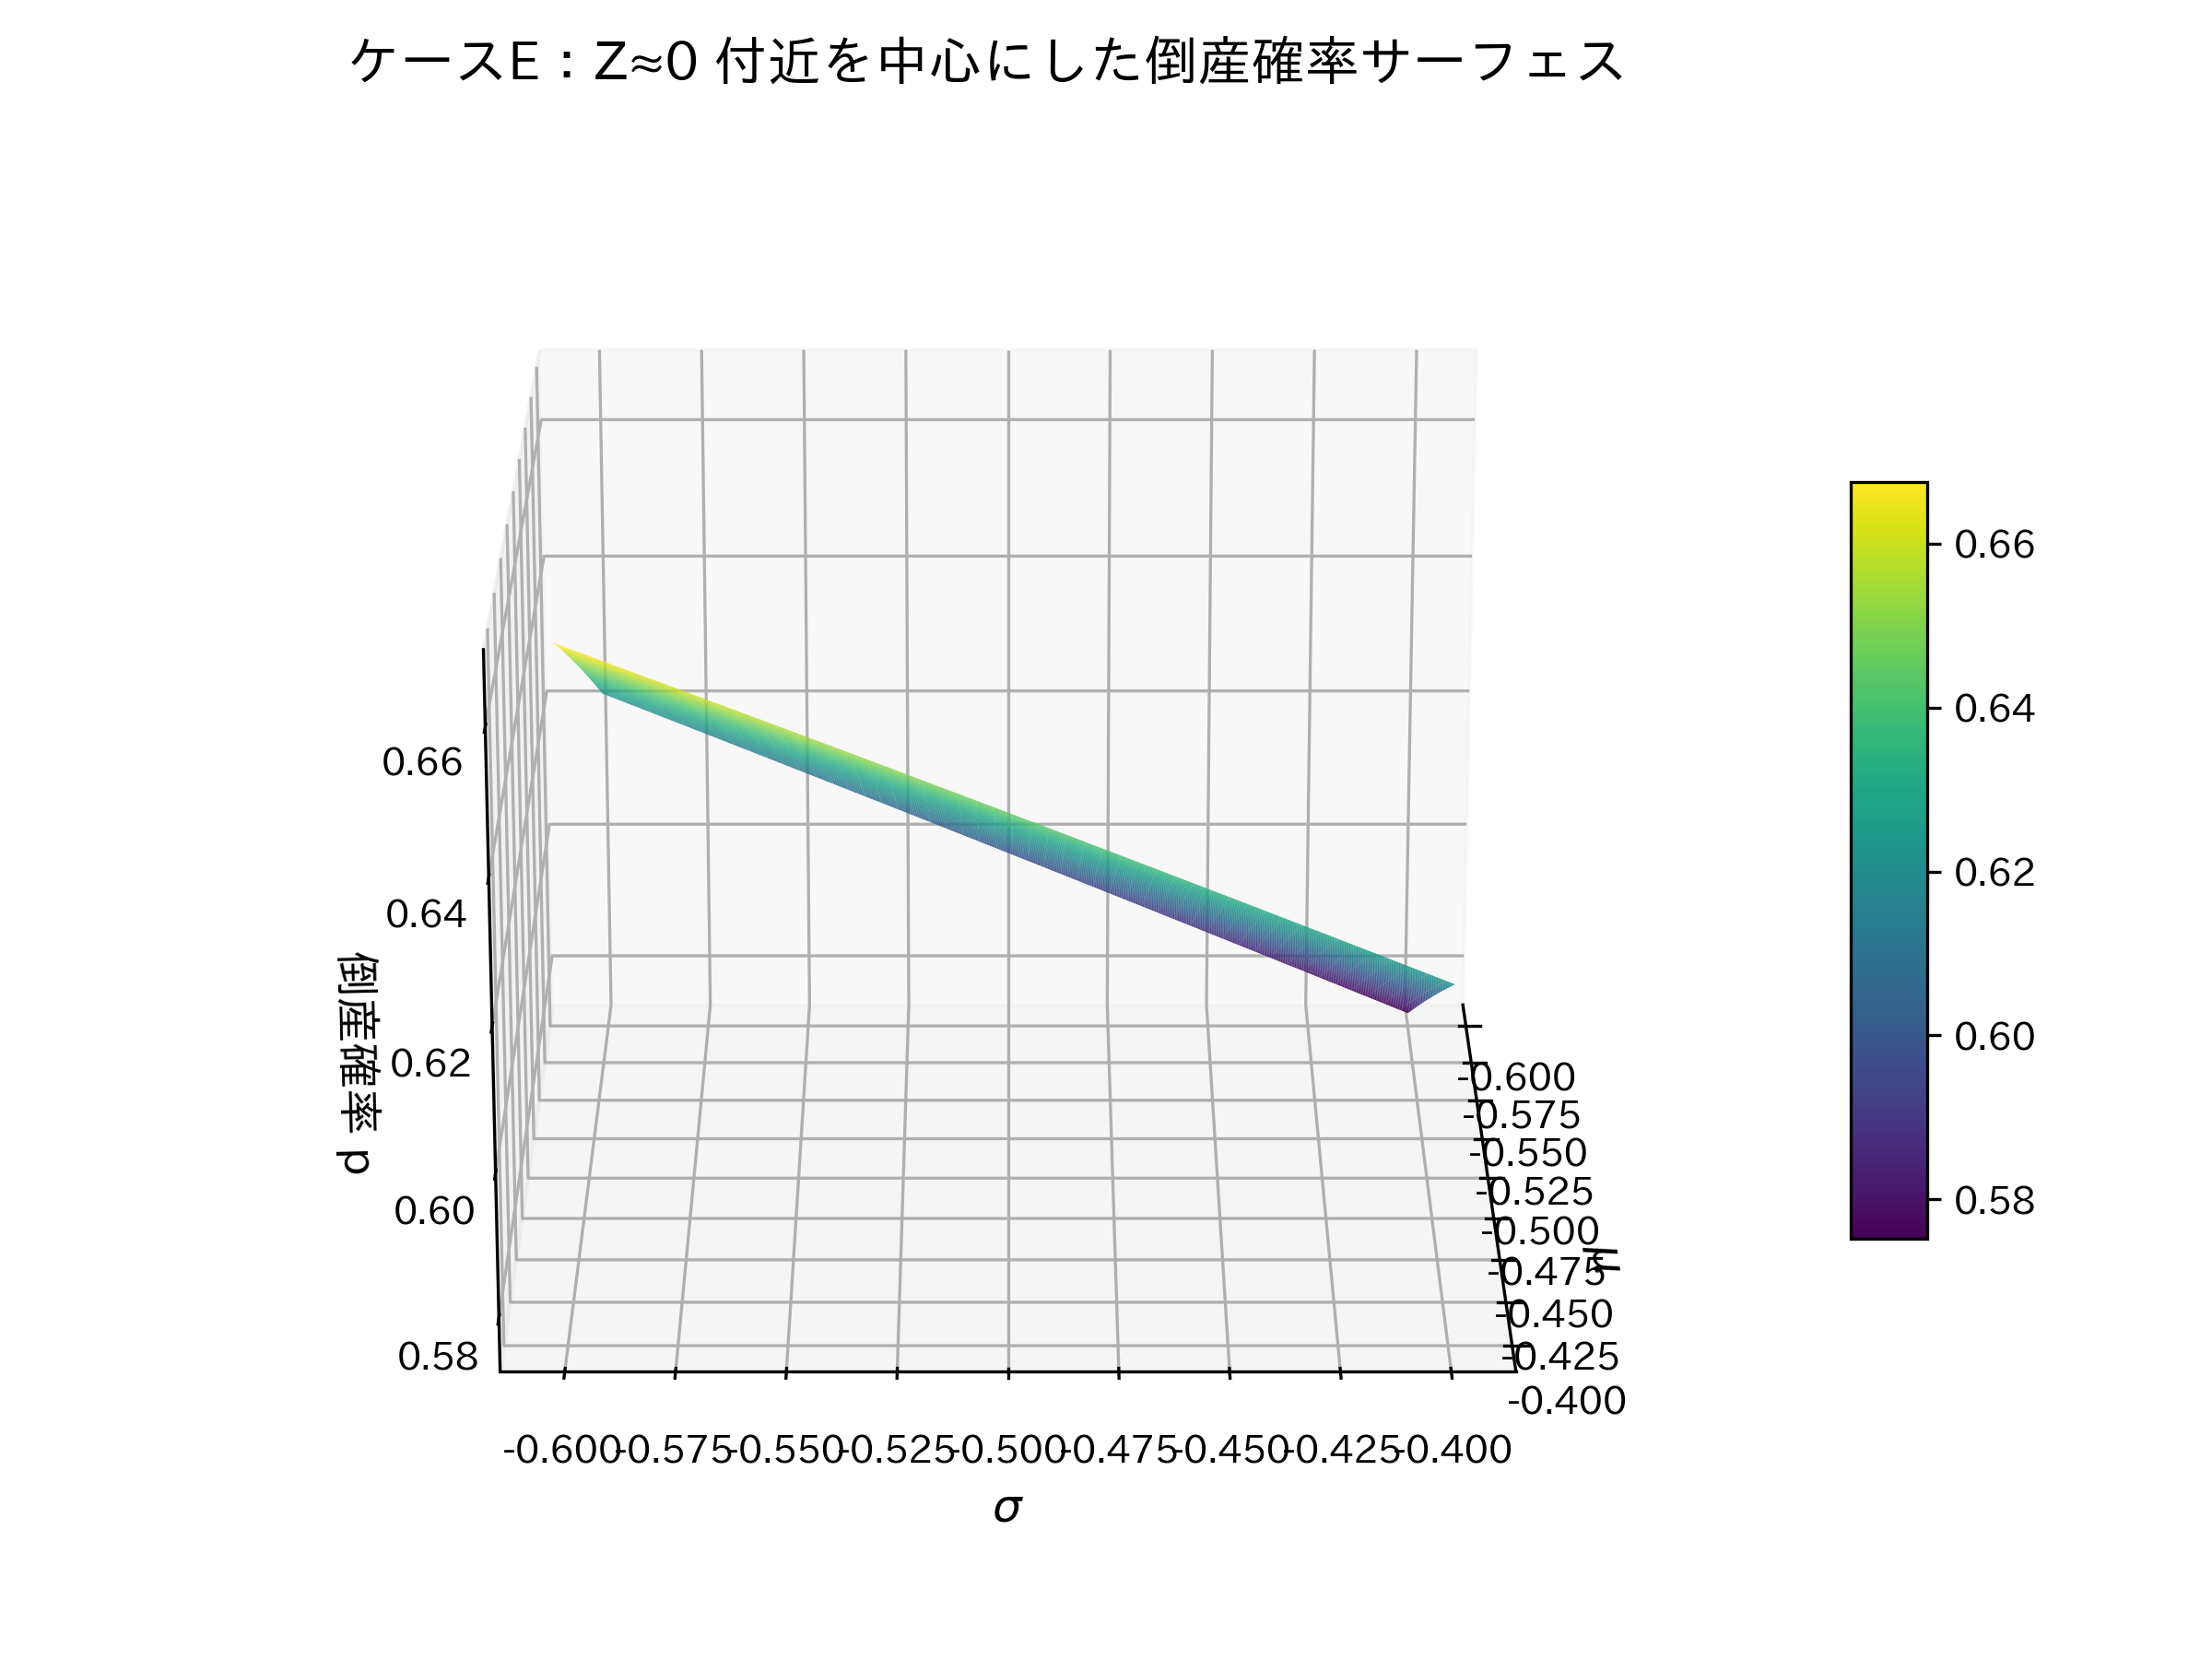
\includegraphics[width=0.75\linewidth]{figures/surface_caseE_centered.png}
    \caption{ケースEにおける倒産確率の3Dサーフェスプロット（Z≈0付近を中心）}
    \label{fig:surface_caseE_centered}
\end{figure}

ケースEは中程度の負債比率と限定的な支援能力を持つ典型的な地域新電力であり，
倒産確率の地形は中間的な位置にある。
Z≈0 を中心に描くことで，
$\mu$ の改善効果が比較的強く，収益性の改善がリスク低下に直結する構造が明確に示される。


% ---------- ケースF ----------
\subsubsection*{ケースF：$D=0.5,\ S=2$（商社系）}

\begin{figure}[H]
    \centering
    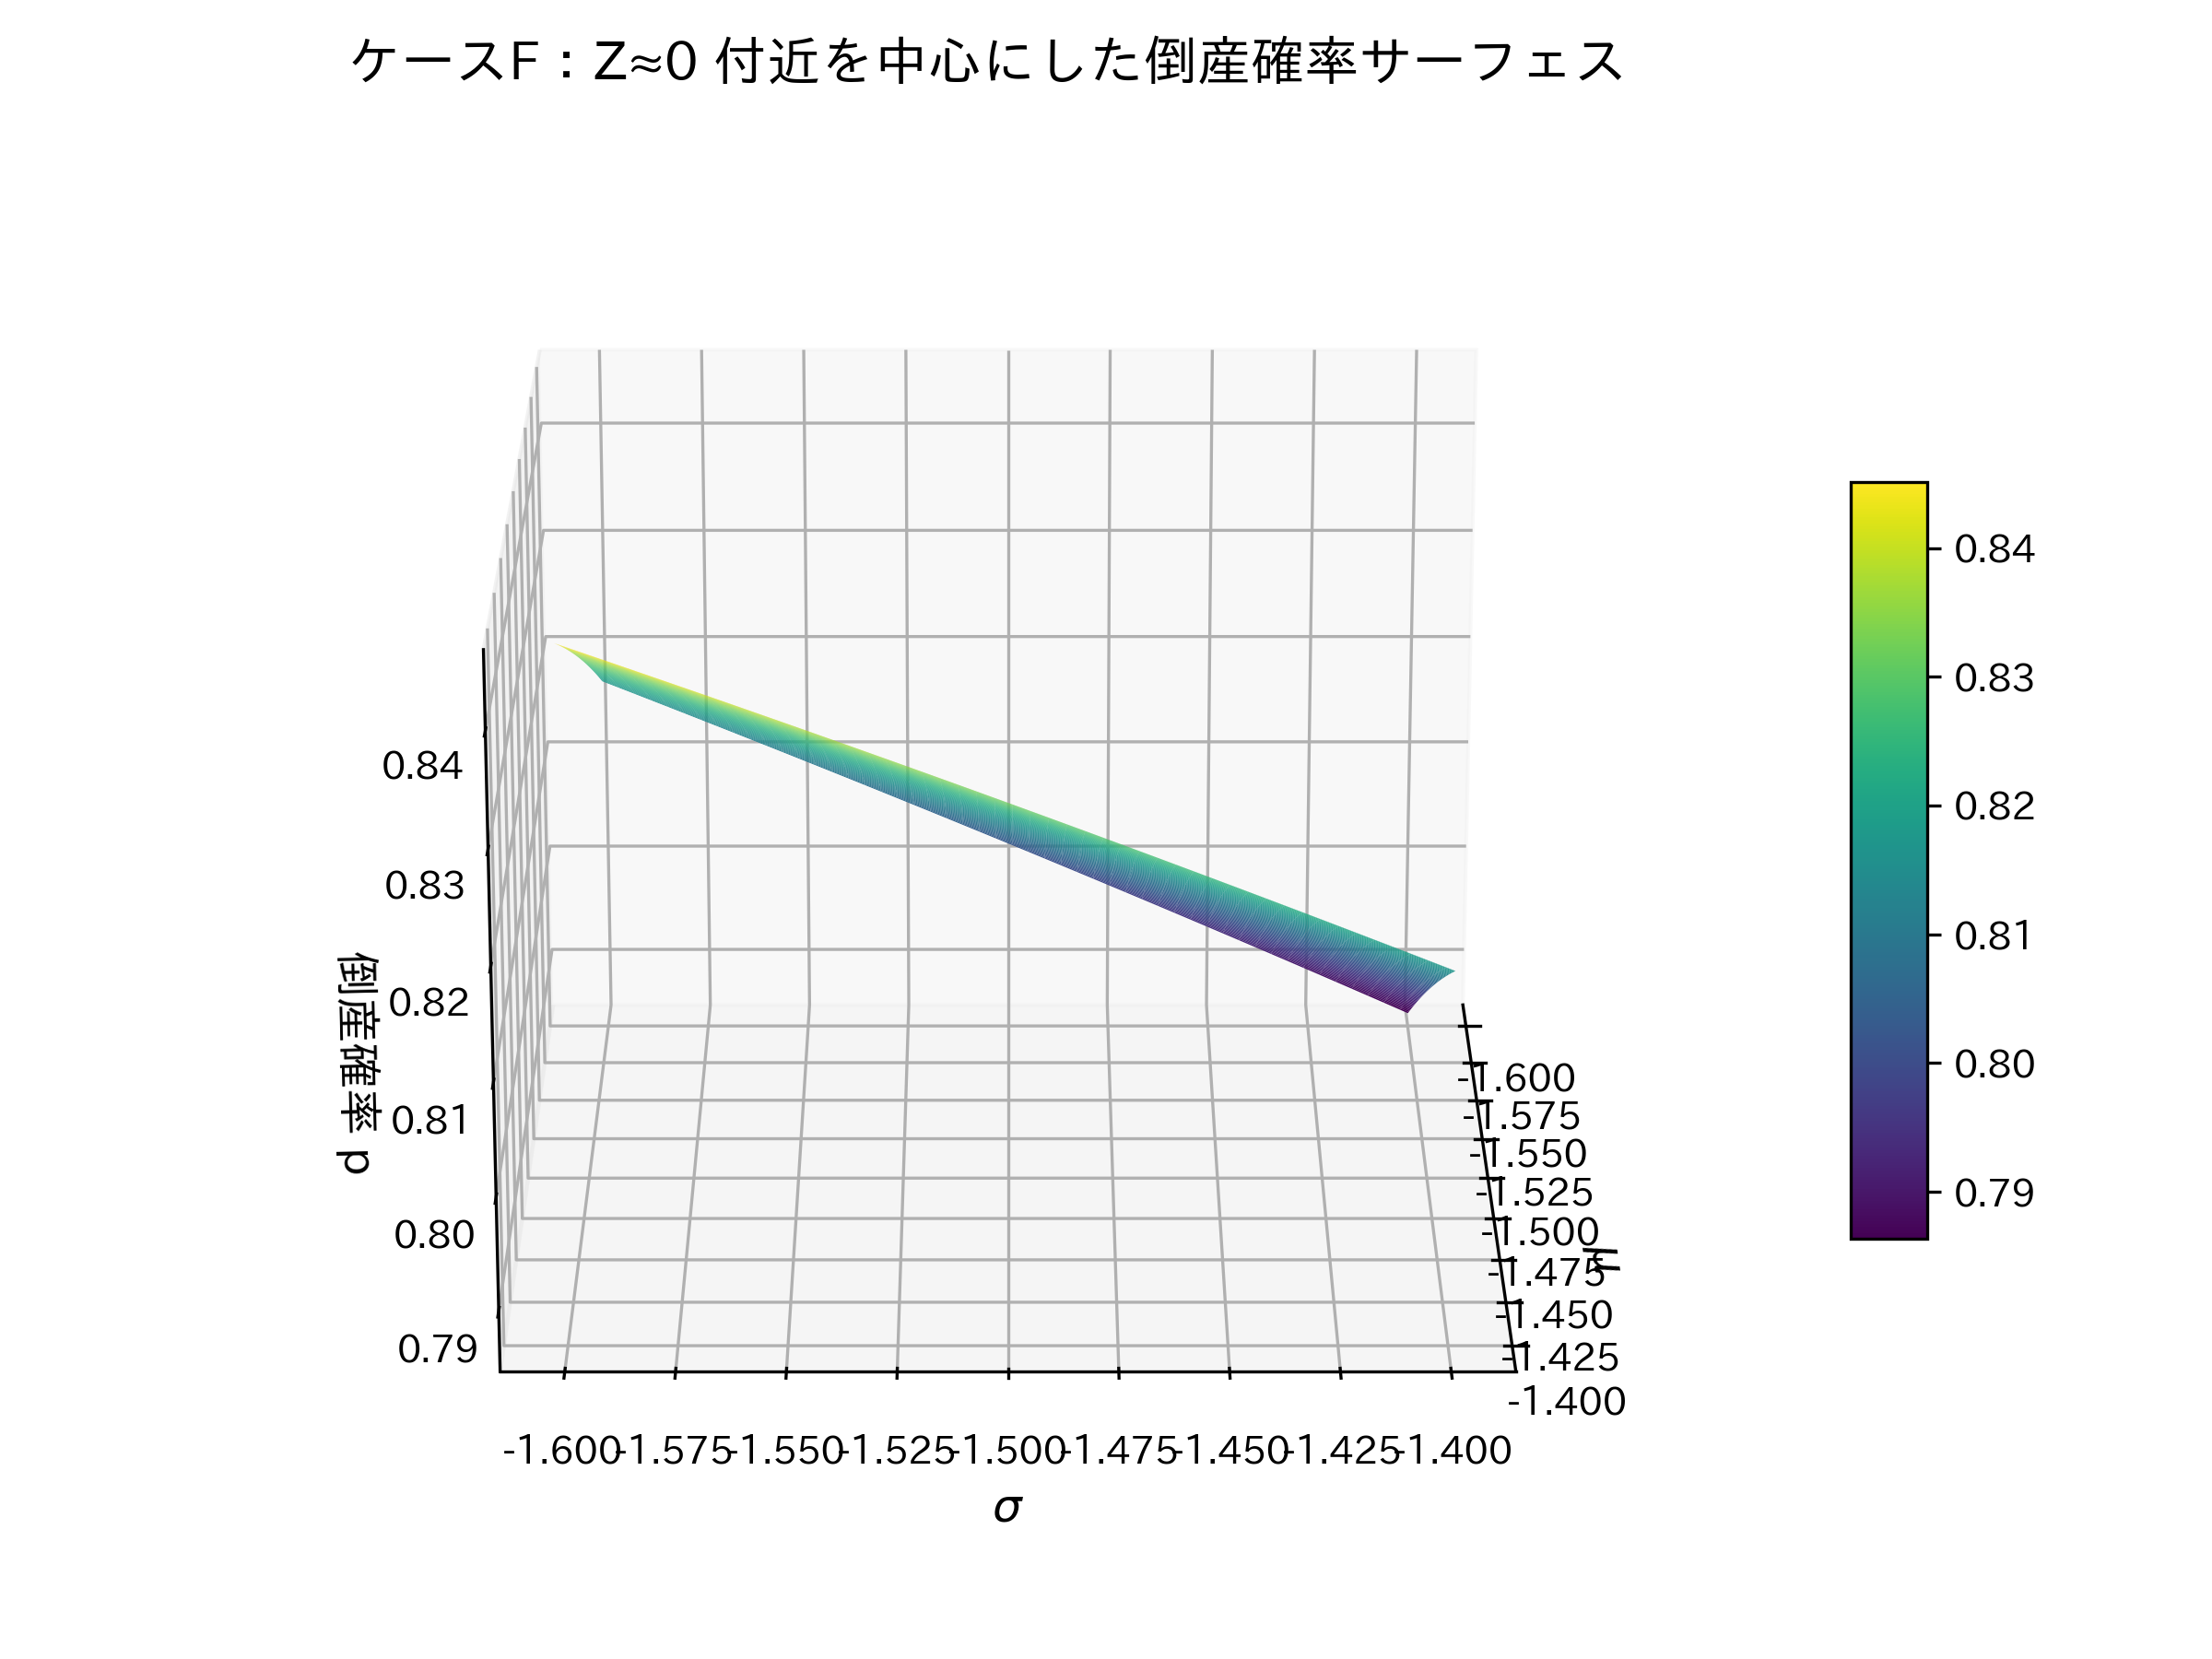
\includegraphics[width=0.75\linewidth]{figures/surface_caseF_centered.png}
    \caption{ケースFにおける倒産確率の3Dサーフェスプロット（Z≈0付近を中心）}
    \label{fig:surface_caseF_centered}
\end{figure}

ケースFでは，商社系の強い支援能力により，
倒産確率の地形はケースEより右方に位置する。
Z≈0 を中心に描くことで，
支援能力が倒産境界線を大きく押し下げる効果が視覚的に確認でき，
外生ショックに対する耐性が向上していることが示される。


\subsection*{大企業と地方電力の倒産リスク格差と，小規模企業が生き残る条件}

本節では，倒産確率の差分


\[
\Delta p = p_{\mathrm{B}} - p_{\mathrm{C}}
\]


を算出し，大企業（ケースB：$D=0.3,\ S=3$）と，
地方電力で資本支援のない企業（ケースC：$D=0.8,\ S=0$）の
倒産リスク格差を可視化する。
図\ref{fig:surface_diff_B_minus_C} に示すとおり，
$\Delta p$ は全域で正となり，
大企業の倒産確率が地方電力より一貫して低いことが確認できる。

\begin{figure}[H]
    \centering
    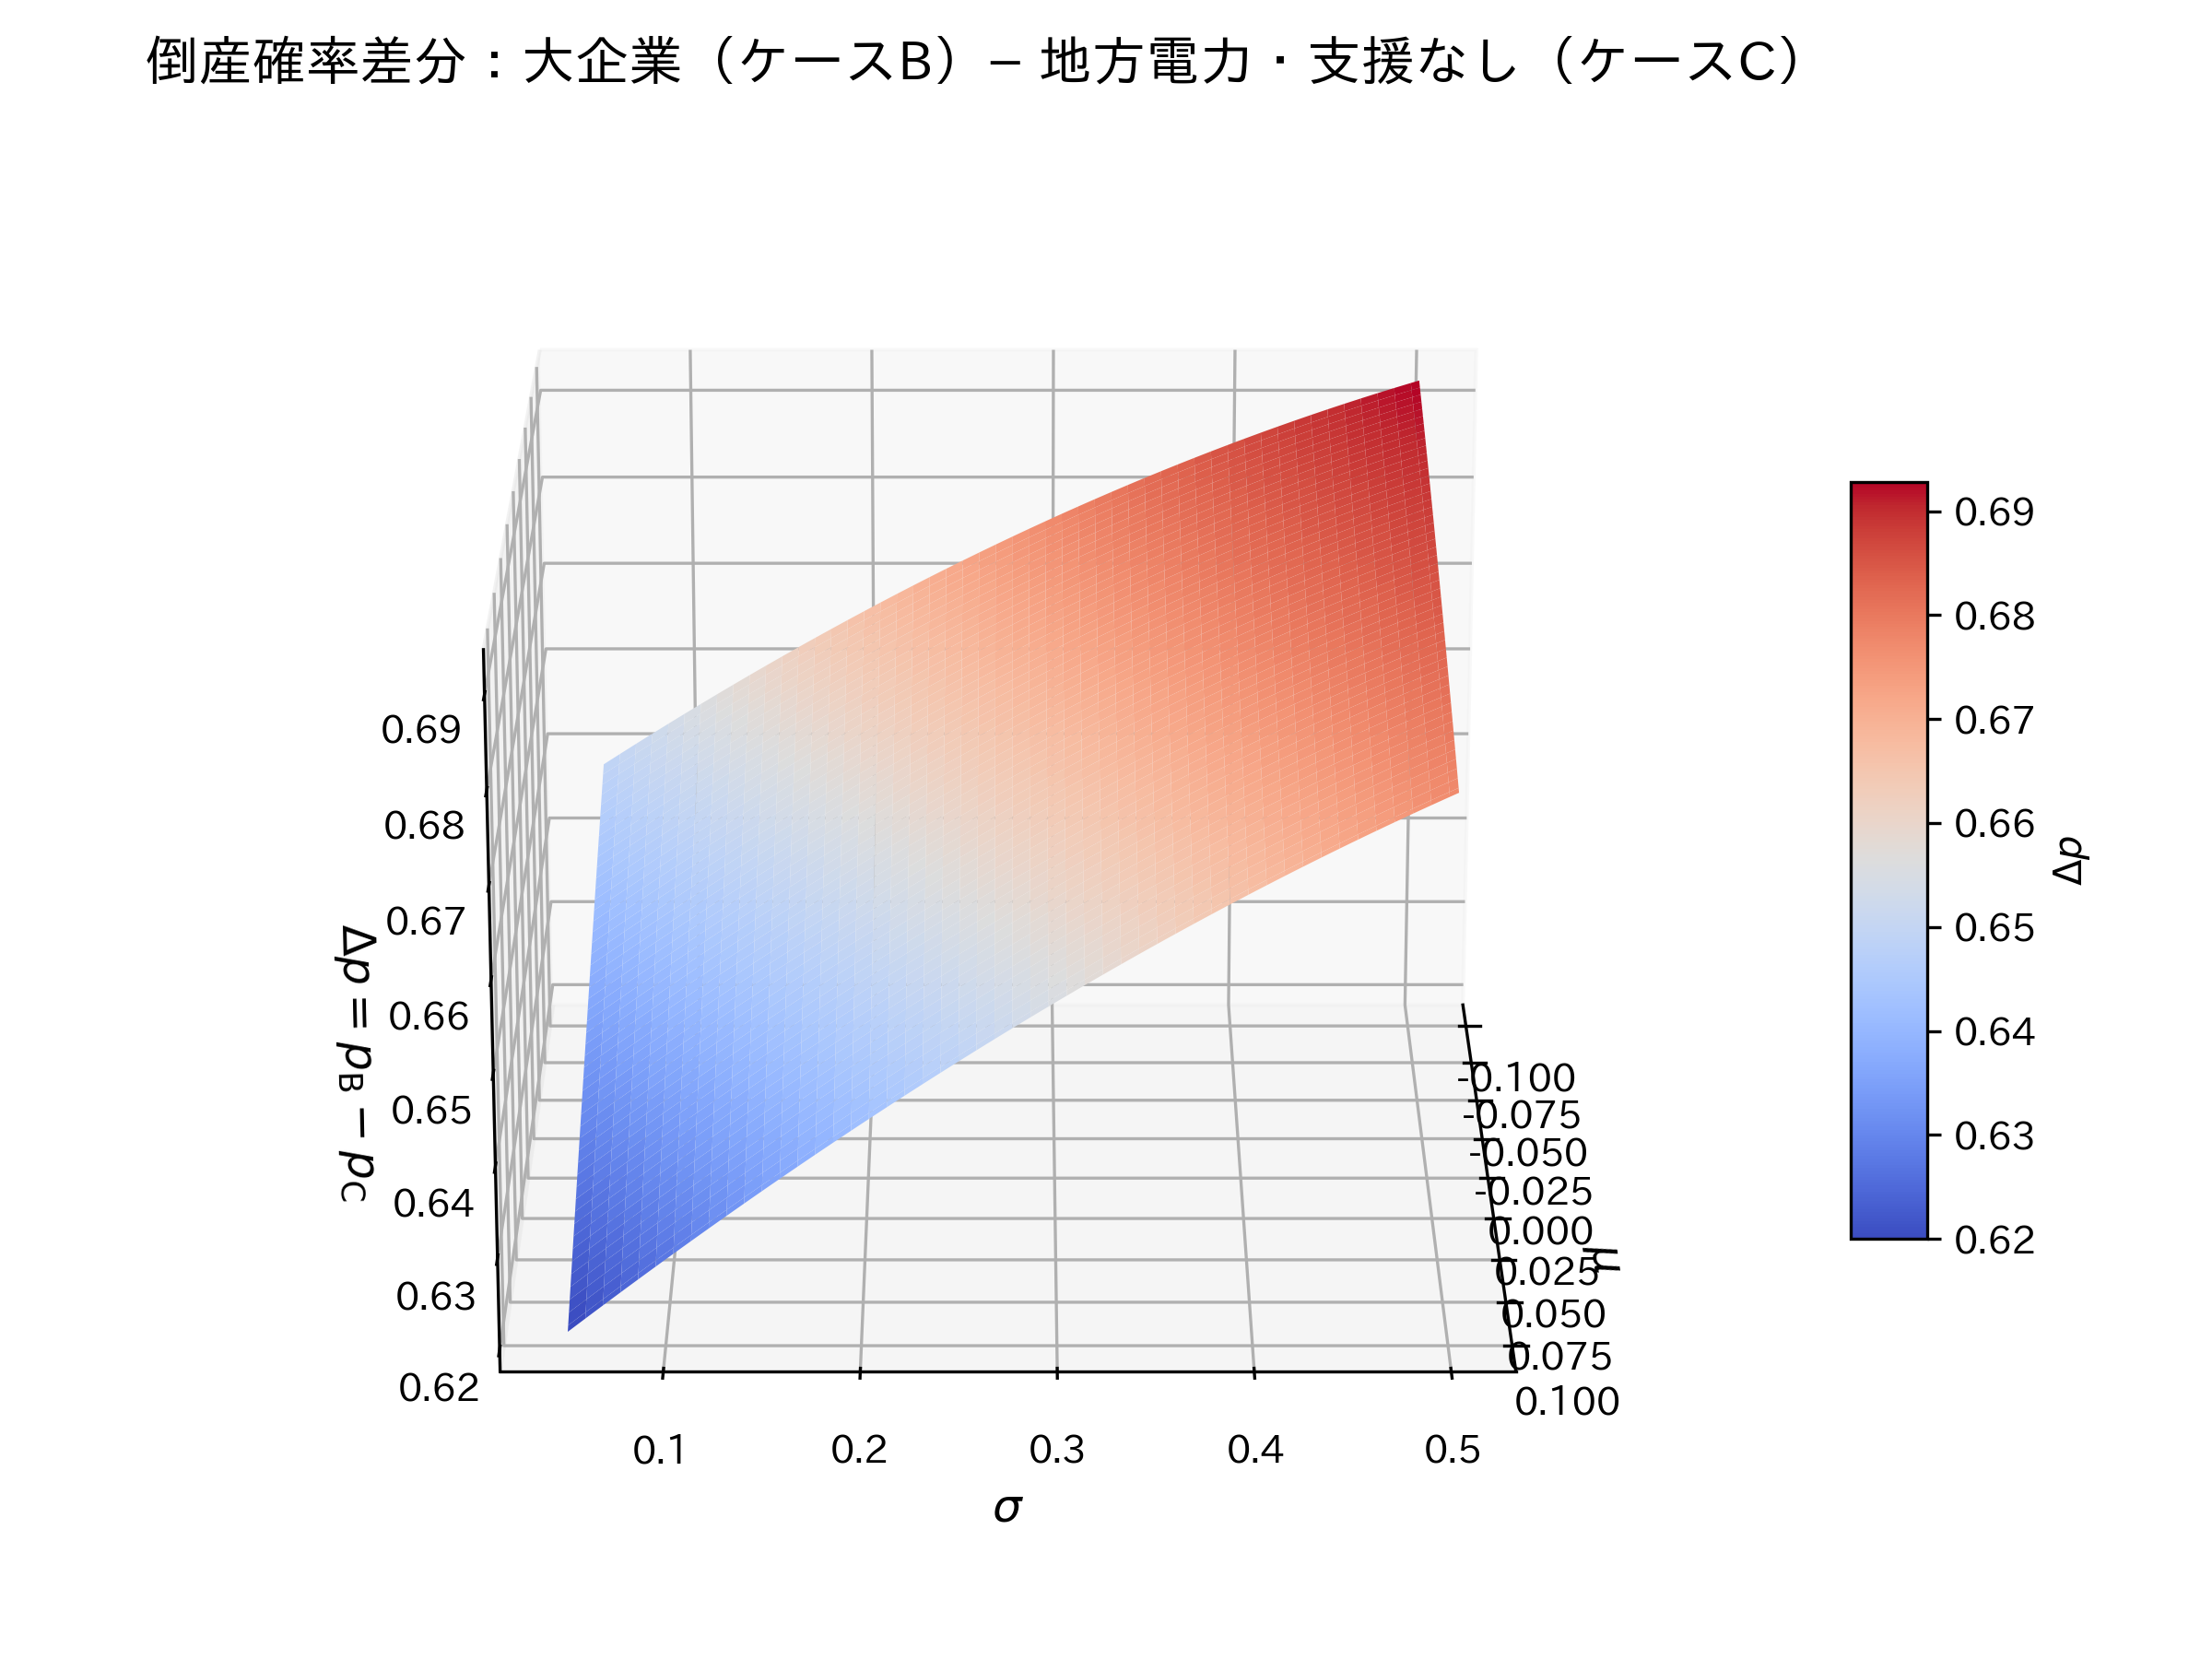
\includegraphics[width=0.75\linewidth]{figures/surface_diff_B_minus_C.png}
    \caption{倒産確率の差分サーフェス：大企業（ケースB）$-$ 地方電力・支援なし（ケースC）}
    \label{fig:surface_diff_B_minus_C}
\end{figure}

図\ref{fig:surface_diff_B_minus_C} の形状は，
倒産リスク格差が $\mu$（収益性）および $\sigma$（市場ショック）の関数として
どのように拡大・縮小するかを示している。
特に以下の3点が重要である。

\begin{enumerate}
    \item \textbf{市場ショックが大きいほど格差が拡大する}  
    $\sigma$ が大きい領域では $\Delta p$ が急速に増加しており，
    市場変動に対する脆弱性が地方電力に集中していることがわかる。
    大企業は支援能力 $S=3$ によりショックを吸収できる一方，
    地方電力は $\sigma$ の上昇に対して倒産確率が急激に上昇する。

    \item \textbf{収益性が低いほど格差が最大化する}  
    $\mu$ が負の領域では $\Delta p$ が最も大きく，
    収益性の低下が地方電力の倒産確率を大幅に押し上げる。
    大企業は $\mu$ が低くても支援能力により倒産確率が抑制されるため，
    両者の差が顕著に現れる。

    \item \textbf{支援能力（$S$）の有無が倒産確率を決定づける}  
    本モデルでは，負債比率 $D$ や収益性 $\mu$ 以上に，
    支援能力 $S$ が倒産確率に強く作用する。
    ケースBとケースCの差分が 0.6〜0.7 程度に達することは，
    支援能力の有無が企業存続に与える影響が極めて大きいことを示している。
\end{enumerate}

以上の結果は，「大企業が倒産しにくい」という自明な事実を確認するだけではなく，
\textbf{小規模企業であっても生き残るための条件が存在する}ことを
数理モデルにより明確に示している点に意義がある。
すなわち，

\begin{itemize}
    \item 収益性 $\mu$ を一定以上確保すること（価格戦略・コスト削減）
    \item 市場ショック $\sigma$ を低減すること（固定価格契約・ヘッジ）
    \item 支援能力 $S$ を部分的にでも確保すること（自治体・地銀・地域企業との連携）
    \item 負債比率 $D$ を抑制すること（過剰借入の回避）
\end{itemize}

が，小規模企業の倒産確率を大幅に低減させる「生存条件」として導かれる。

本章のシミュレーションは，
大企業と地方電力の倒産リスク格差を定量的に示すとともに，
小規模企業がどのような条件下で生き残り得るのかを
$\mu,\ \sigma,\ S,\ D$ の関数として明確に示した点に学術的意義がある。


% ============================================================
\subsection*{地域新電力と商社系の倒産リスク格差：支援能力の効果}

次に，中規模企業における倒産リスクの構造を明確化するため，
地域新電力（ケースE：$D=0.5,\ S=1$）と，
商社系新電力（ケースF：$D=0.5,\ S=2$）の差分


\[
\Delta p = p_{\mathrm{F}} - p_{\mathrm{E}}
\]


を算出する。
両者は負債比率 $D$ が同一であるため，
支援能力 $S$ の違いが倒産確率にどのように作用するかを
純粋に比較できる点に特徴がある。

\begin{figure}[H]
    \centering
    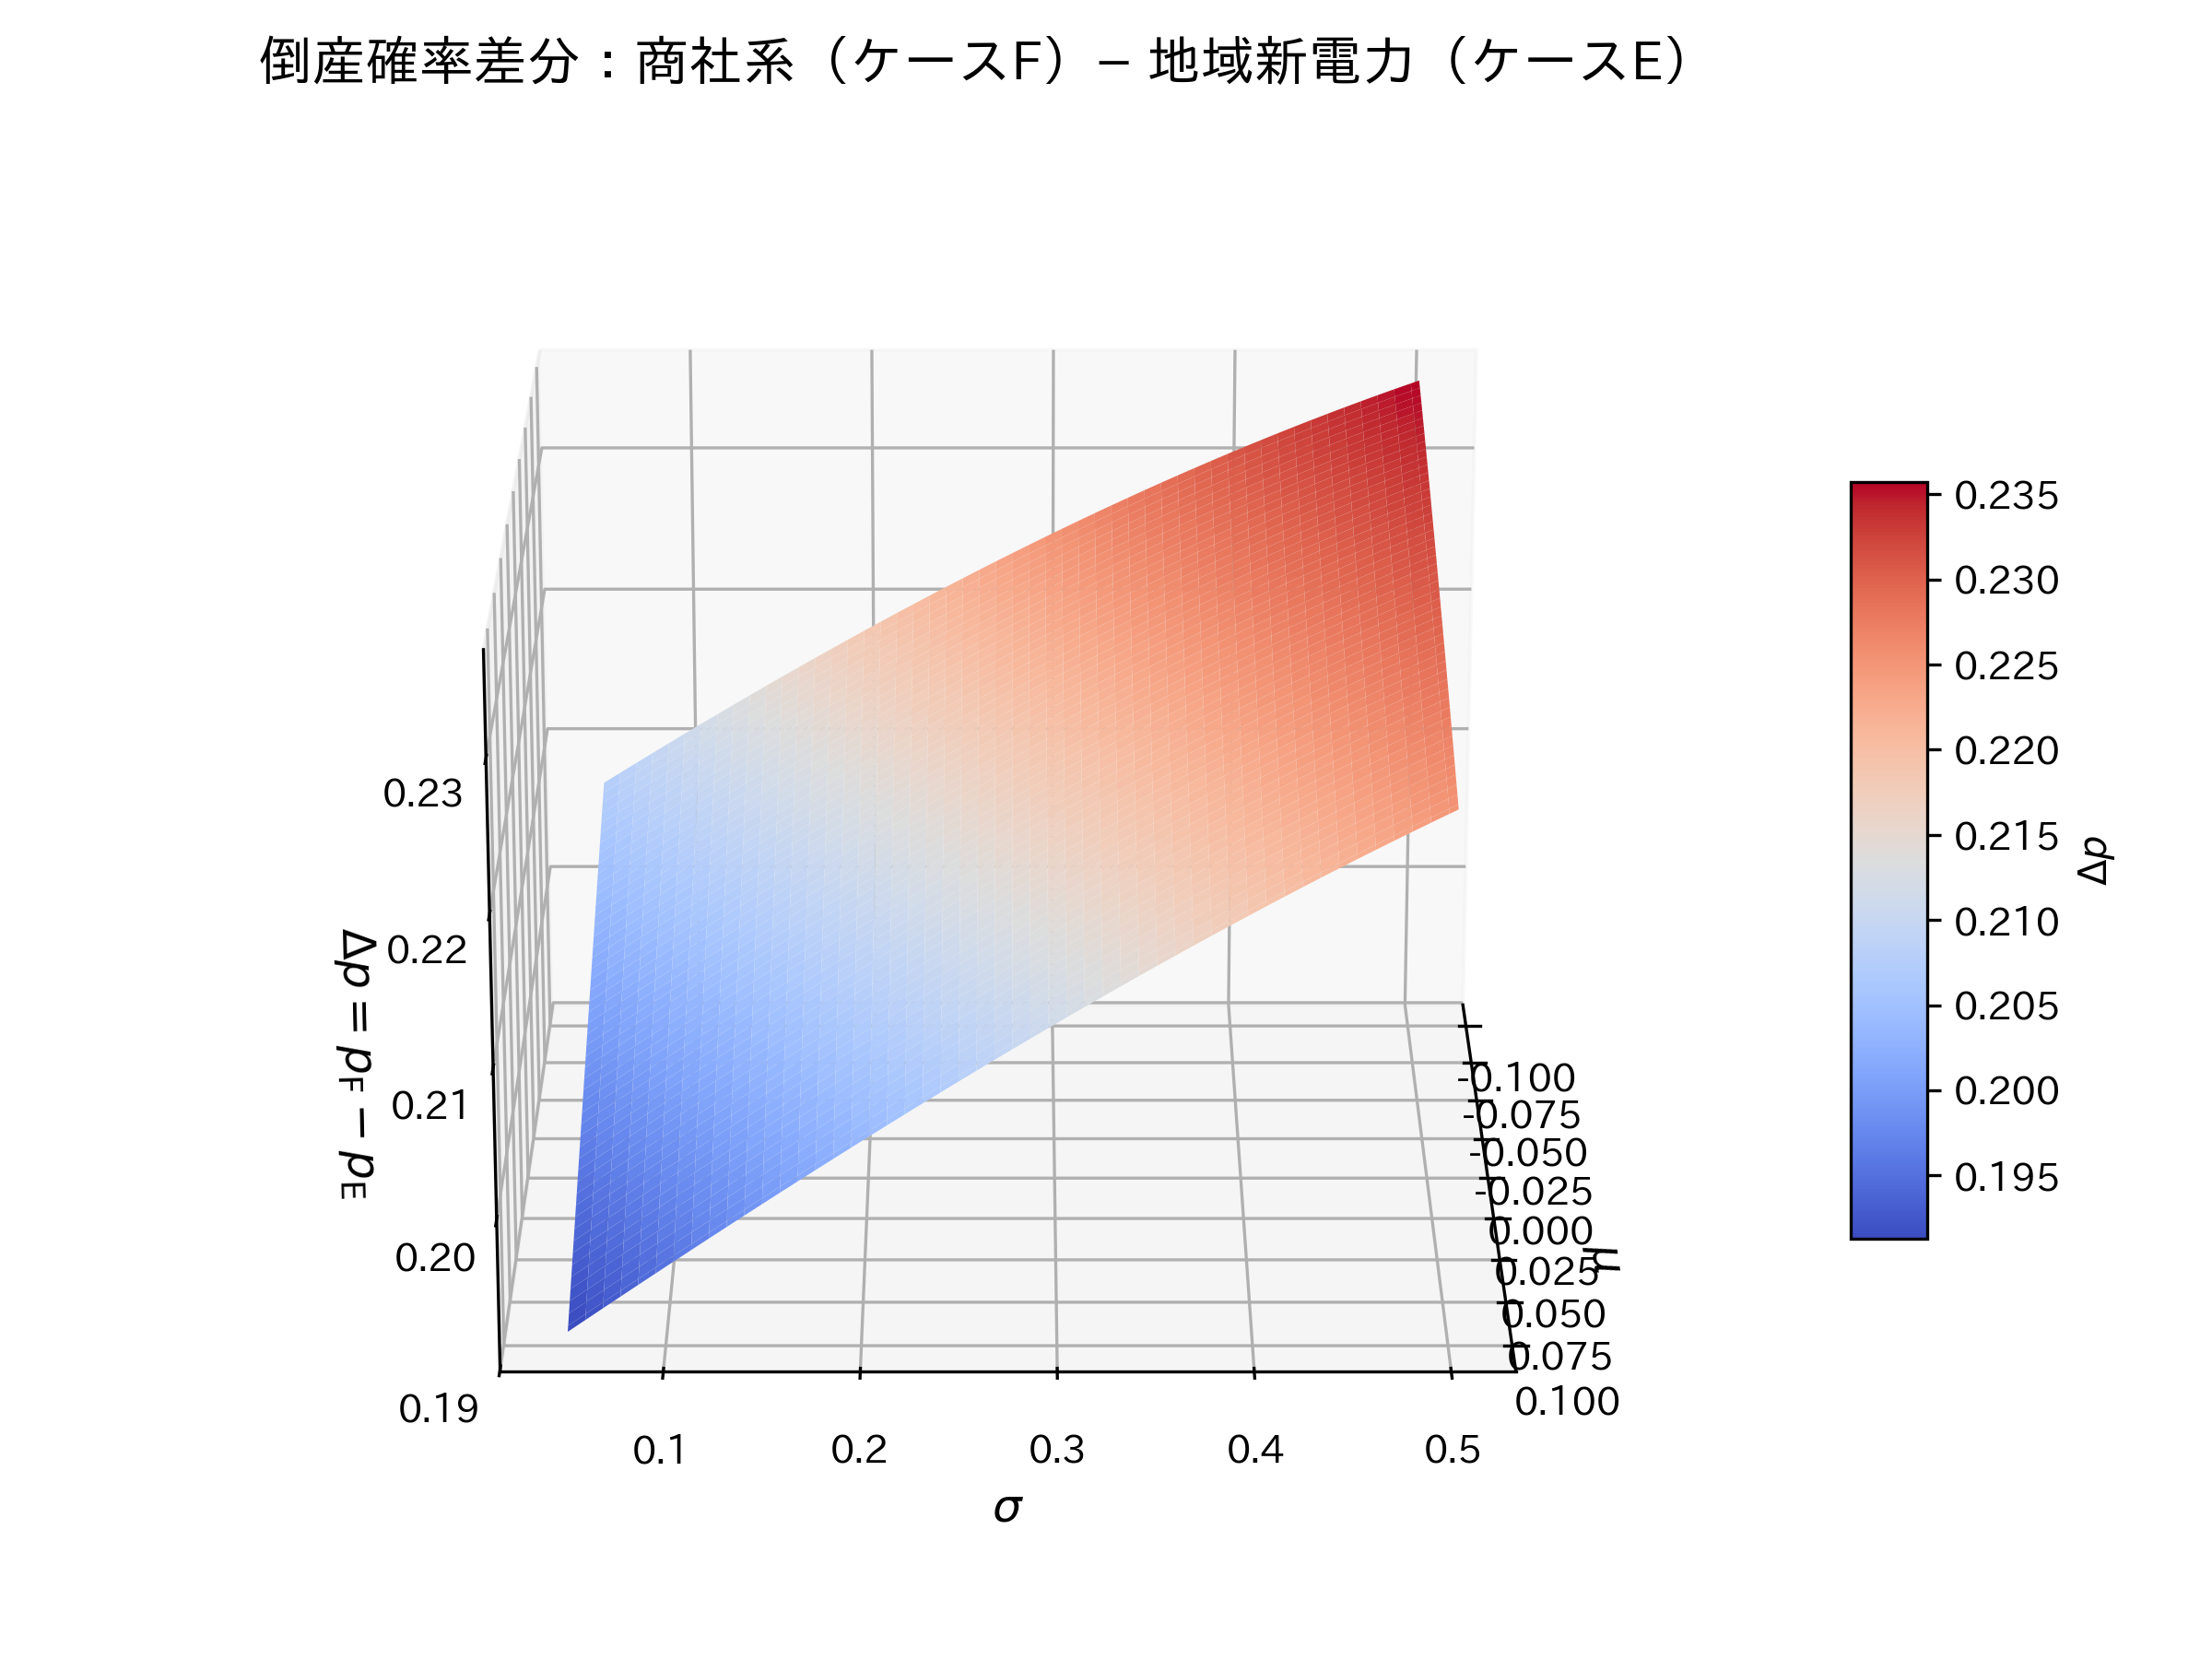
\includegraphics[width=0.75\linewidth]{figures/surface_diff_F_minus_E.png}
    \caption{倒産確率の差分サーフェス：商社系（ケースF）$-$ 地域新電力（ケースE）}
    \label{fig:surface_diff_F_minus_E}
\end{figure}

図\ref{fig:surface_diff_F_minus_E} に示すとおり，
$\Delta p$ は全域で正となり，
商社系（ケースF）の倒産確率が地域新電力（ケースE）より一貫して低いことが確認できる。
特に以下の3点が重要である。

\begin{enumerate}
    \item \textbf{市場ショックが大きいほど格差が拡大する}  
    $\sigma$ が大きい領域では $\Delta p$ が急速に増加しており，
    市場変動に対する耐性が支援能力 $S$ の差によって大きく左右されることがわかる。

    \item \textbf{収益性が低いほど支援能力の効果が強く現れる}  
    $\mu$ が負の領域では $\Delta p$ が最大化し，
    収益性の低下が地域新電力の倒産確率を大きく押し上げる一方，
    商社系は支援能力 $S=2$ により倒産確率の上昇が抑制される。

    \item \textbf{支援能力 $S$ の上昇は，中規模企業においても倒産確率を大幅に低減する}  
    ケースEとケースFの差分は 0.2〜0.3 程度であり，
    大企業と地方電力の比較（0.6〜0.7）ほど極端ではないものの，
    中規模企業においても支援能力が倒産確率に与える影響は決定的である。
\end{enumerate}

以上の結果は，
「企業規模が小さいほど倒産しやすい」という単純な構図ではなく，
\textbf{支援能力 $S$ が部分的にでも確保されれば，
中規模企業であっても倒産リスクを大幅に低減できる}
ことを示している。
すなわち，地域新電力の生存可能性は，


\[
(\mu,\ \sigma,\ D) \text{ に加えて } S \text{ をいかに確保できるか}
\]


に強く依存しており，
自治体・地銀・地域企業との連携やスポンサー支援の獲得が
実務的な生存戦略として極めて重要である。




% ============================================================
\subsection{ケース横断的な比較と含意}
% ------------------------------------------------------------
% ・ケースA〜Fの共通点と相違点を体系的に整理する
% ・S と D の影響を統合的に評価する
% ・第7章の実証分析への橋渡しを行う
% ------------------------------------------------------------

ケースA〜Fの比較から，以下の統合的な特徴が確認される。

\begin{itemize}
    \item 支援能力 $S$ の上昇は，倒産確率の地形全体を右方へ移動させ，
          外生ショックに対する耐性を高める。
    \item 負債比率 $D$ の上昇は，倒産確率の立ち上がりを急峻にし，
          高ボラティリティ環境での脆弱性を増幅する。
    \item 収益性 $\mu$ の改善効果は，負債比率が高い企業ほど大きく，
          財務的に脆弱な企業ほど収益性の改善が倒産確率低下に直結する。
\end{itemize}

これらの特徴は，第4章で導出した理論モデルの符号条件と整合的であるだけでなく，
新電力企業の倒産事例で指摘されてきたリスク要因
（収益性の低下，外生ショック，スポンサー支援の有無，負債過多）
を構造的に再現している。
次章では，これらの理論的含意を踏まえつつ，
実際の財務データを用いた実証分析を行い，
$Z_{\text{lin}}$ の予測性能と現実的な適用可能性を検証する。

% ============================================================
% 7.7 B&S 型倒産リスクシミュレーション
% ------------------------------------------------------------
% ・B&S 型ロジット式に基づき，新電力の代表パターンごとの倒産確率を算出
% ・第6章前半の Merton 型シミュレーションと比較し，リスク構造の整合性を確認
% ・第7章の実証分析で用いる B&S 型モデルの直感的含意を整理
% ============================================================

\section{B\&S 型倒産リスクシミュレーション}
\label{sec:bs_risk_simulation}

本節では，Bharath and Shumway（2008）に代表される reduced-form 型の
倒産確率モデルを，新電力企業の文脈に適用した場合の挙動をシミュレーションにより確認する。
具体的には，第5章で定義した収益性 $\mu$，市場ショック $\sigma$，
支援能力 $S$，負債比率 $D$ を説明変数とする B\&S 型ロジット式を用いて，
第6章前半で設定した新電力の代表的な財務プロファイル（ケースA〜F）ごとに
倒産確率を算出し，Merton 型シミュレーションの結果と比較する。

この分析の目的は，第7章で用いる B\&S 型ロジットモデルが，
Merton 型理論モデルと同様のリスク構造（$\mu$，$\sigma$，$S$，$D$ の符号条件や
相対的重要度）を再現しているかを確認し，
実証分析におけるモデル選択の直感的な裏付けを与えることである。

% ------------------------------------------------------------
\subsection{B\&S 型ロジットモデルの仕様}

本節で用いる倒産確率モデルは，次のロジット形式で与えられる。



\[
\text{logit}(p_i)
= \alpha + \beta_{\mu} \mu_i + \beta_{\sigma} \sigma_i
  + \beta_{S} S_i + \beta_{D} D_i,
\]





\[
p_i = \frac{1}{1 + \exp\bigl(-\{\alpha + \beta_{\mu} \mu_i
  + \beta_{\sigma} \sigma_i + \beta_{S} S_i + \beta_{D} D_i\}\bigr)}.
\]



係数は，第4章および第6章前半で確認した符号条件と整合的になるように設定する。



\[
\alpha = 0.0,\quad
\beta_{\mu} = -4.0,\quad
\beta_{\sigma} = 3.0,\quad
\beta_{S} = -0.8,\quad
\beta_{D} = 2.0.
\]



% ------------------------------------------------------------
\subsection{新電力の代表ケースの設定}

第6章前半と同様に，新電力企業の典型的な財務状態を反映した
6つの代表ケース（A〜F）を用いる。

\begin{itemize}
    \item ケースA：$D=0.3,\ S=0$（独立系・財務健全）
    \item ケースB：$D=0.3,\ S=3$（大手系・財務健全）
    \item ケースC：$D=0.8,\ S=0$（独立系・負債過多）
    \item ケースD：$D=0.8,\ S=3$（大手系・負債過多）
    \item ケースE：$D=0.5,\ S=1$（地域新電力）
    \item ケースF：$D=0.5,\ S=2$（商社系）
\end{itemize}

収益性 $\mu$ と市場ショック $\sigma$ は以下の範囲で連続的に変化させる。



\[
\mu \in [-0.10, 0.10],\qquad
\sigma \in [0.05, 0.50].
\]



% ------------------------------------------------------------
\subsection{倒産確率サーフェスの可視化}

以下では，ケースA〜Fについて，
B\&S 型ロジットモデルに基づく倒産確率サーフェスを示す。

% ---------- ケースA ----------
\subsubsection*{ケースA：$D=0.3,\ S=0$（独立系・財務健全）}

\begin{figure}[H]
    \centering
    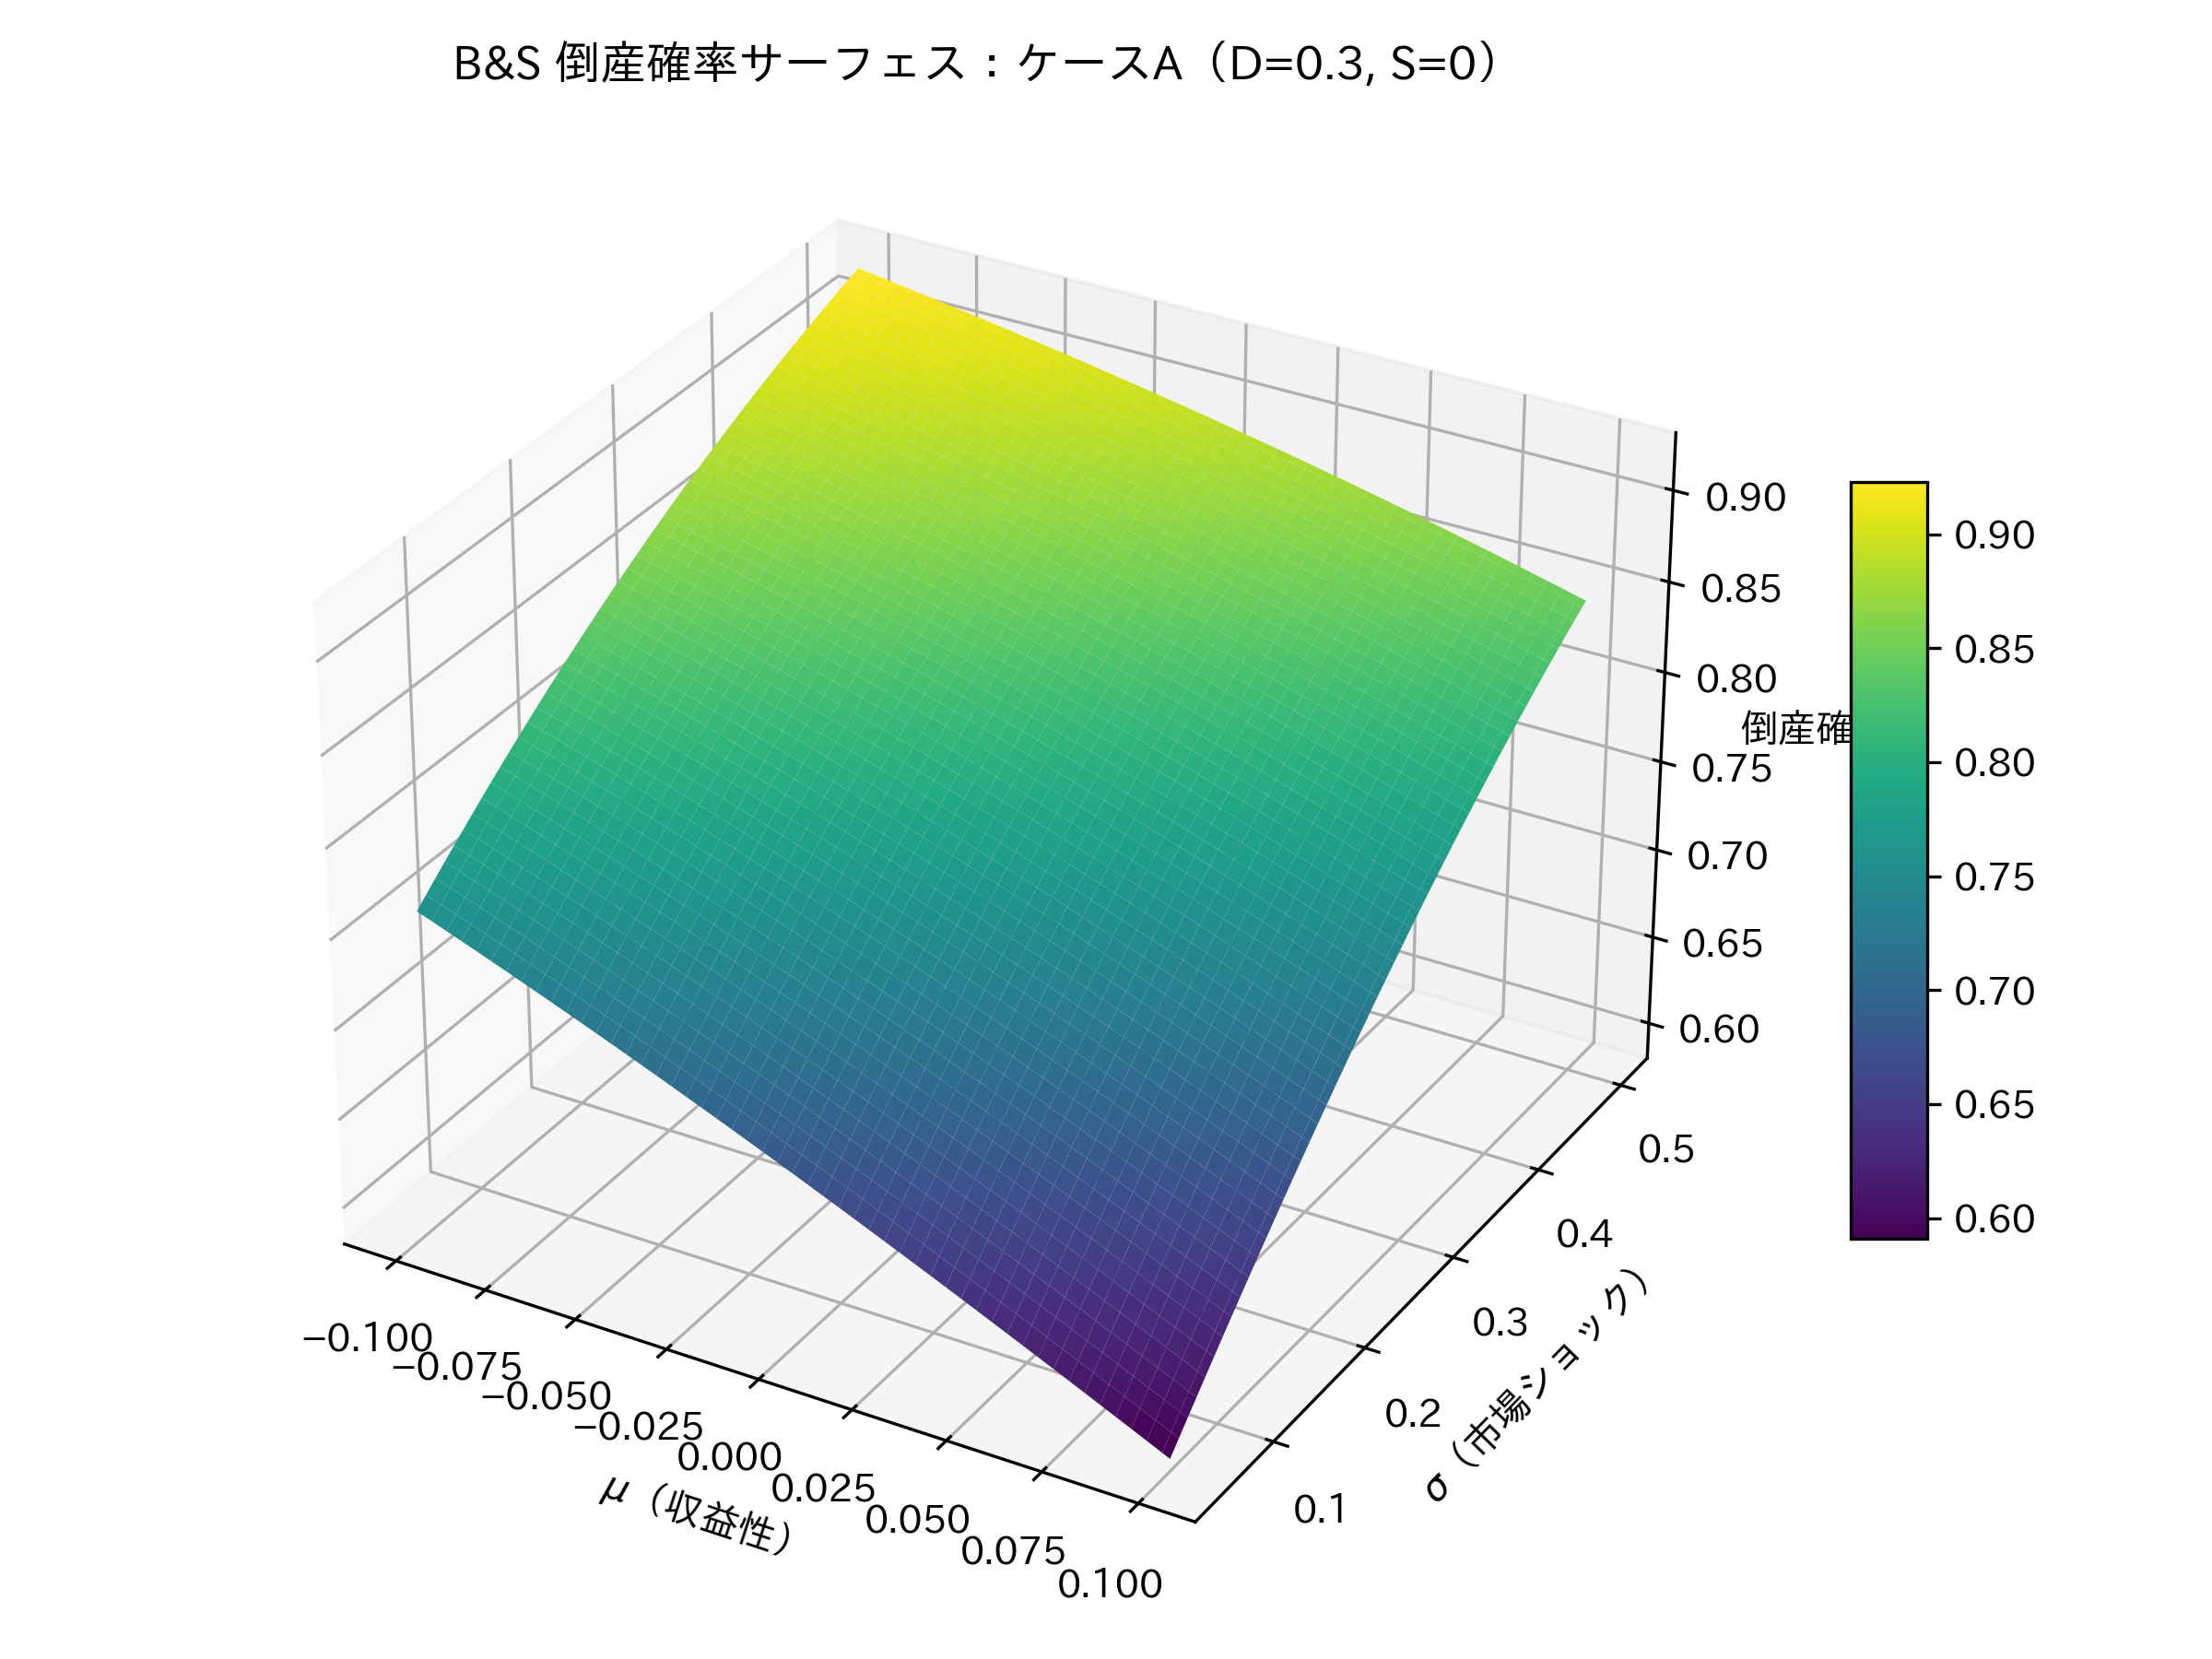
\includegraphics[width=0.75\linewidth]{figures/bs_surface_caseA.png}
    \caption{B\&S 型倒産確率サーフェス：ケースA（独立系・財務健全）}
    \label{fig:bs_surface_caseA}
\end{figure}

% ---------- ケースB ----------
\subsubsection*{ケースB：$D=0.3,\ S=3$（大手系・財務健全）}

\begin{figure}[H]
    \centering
    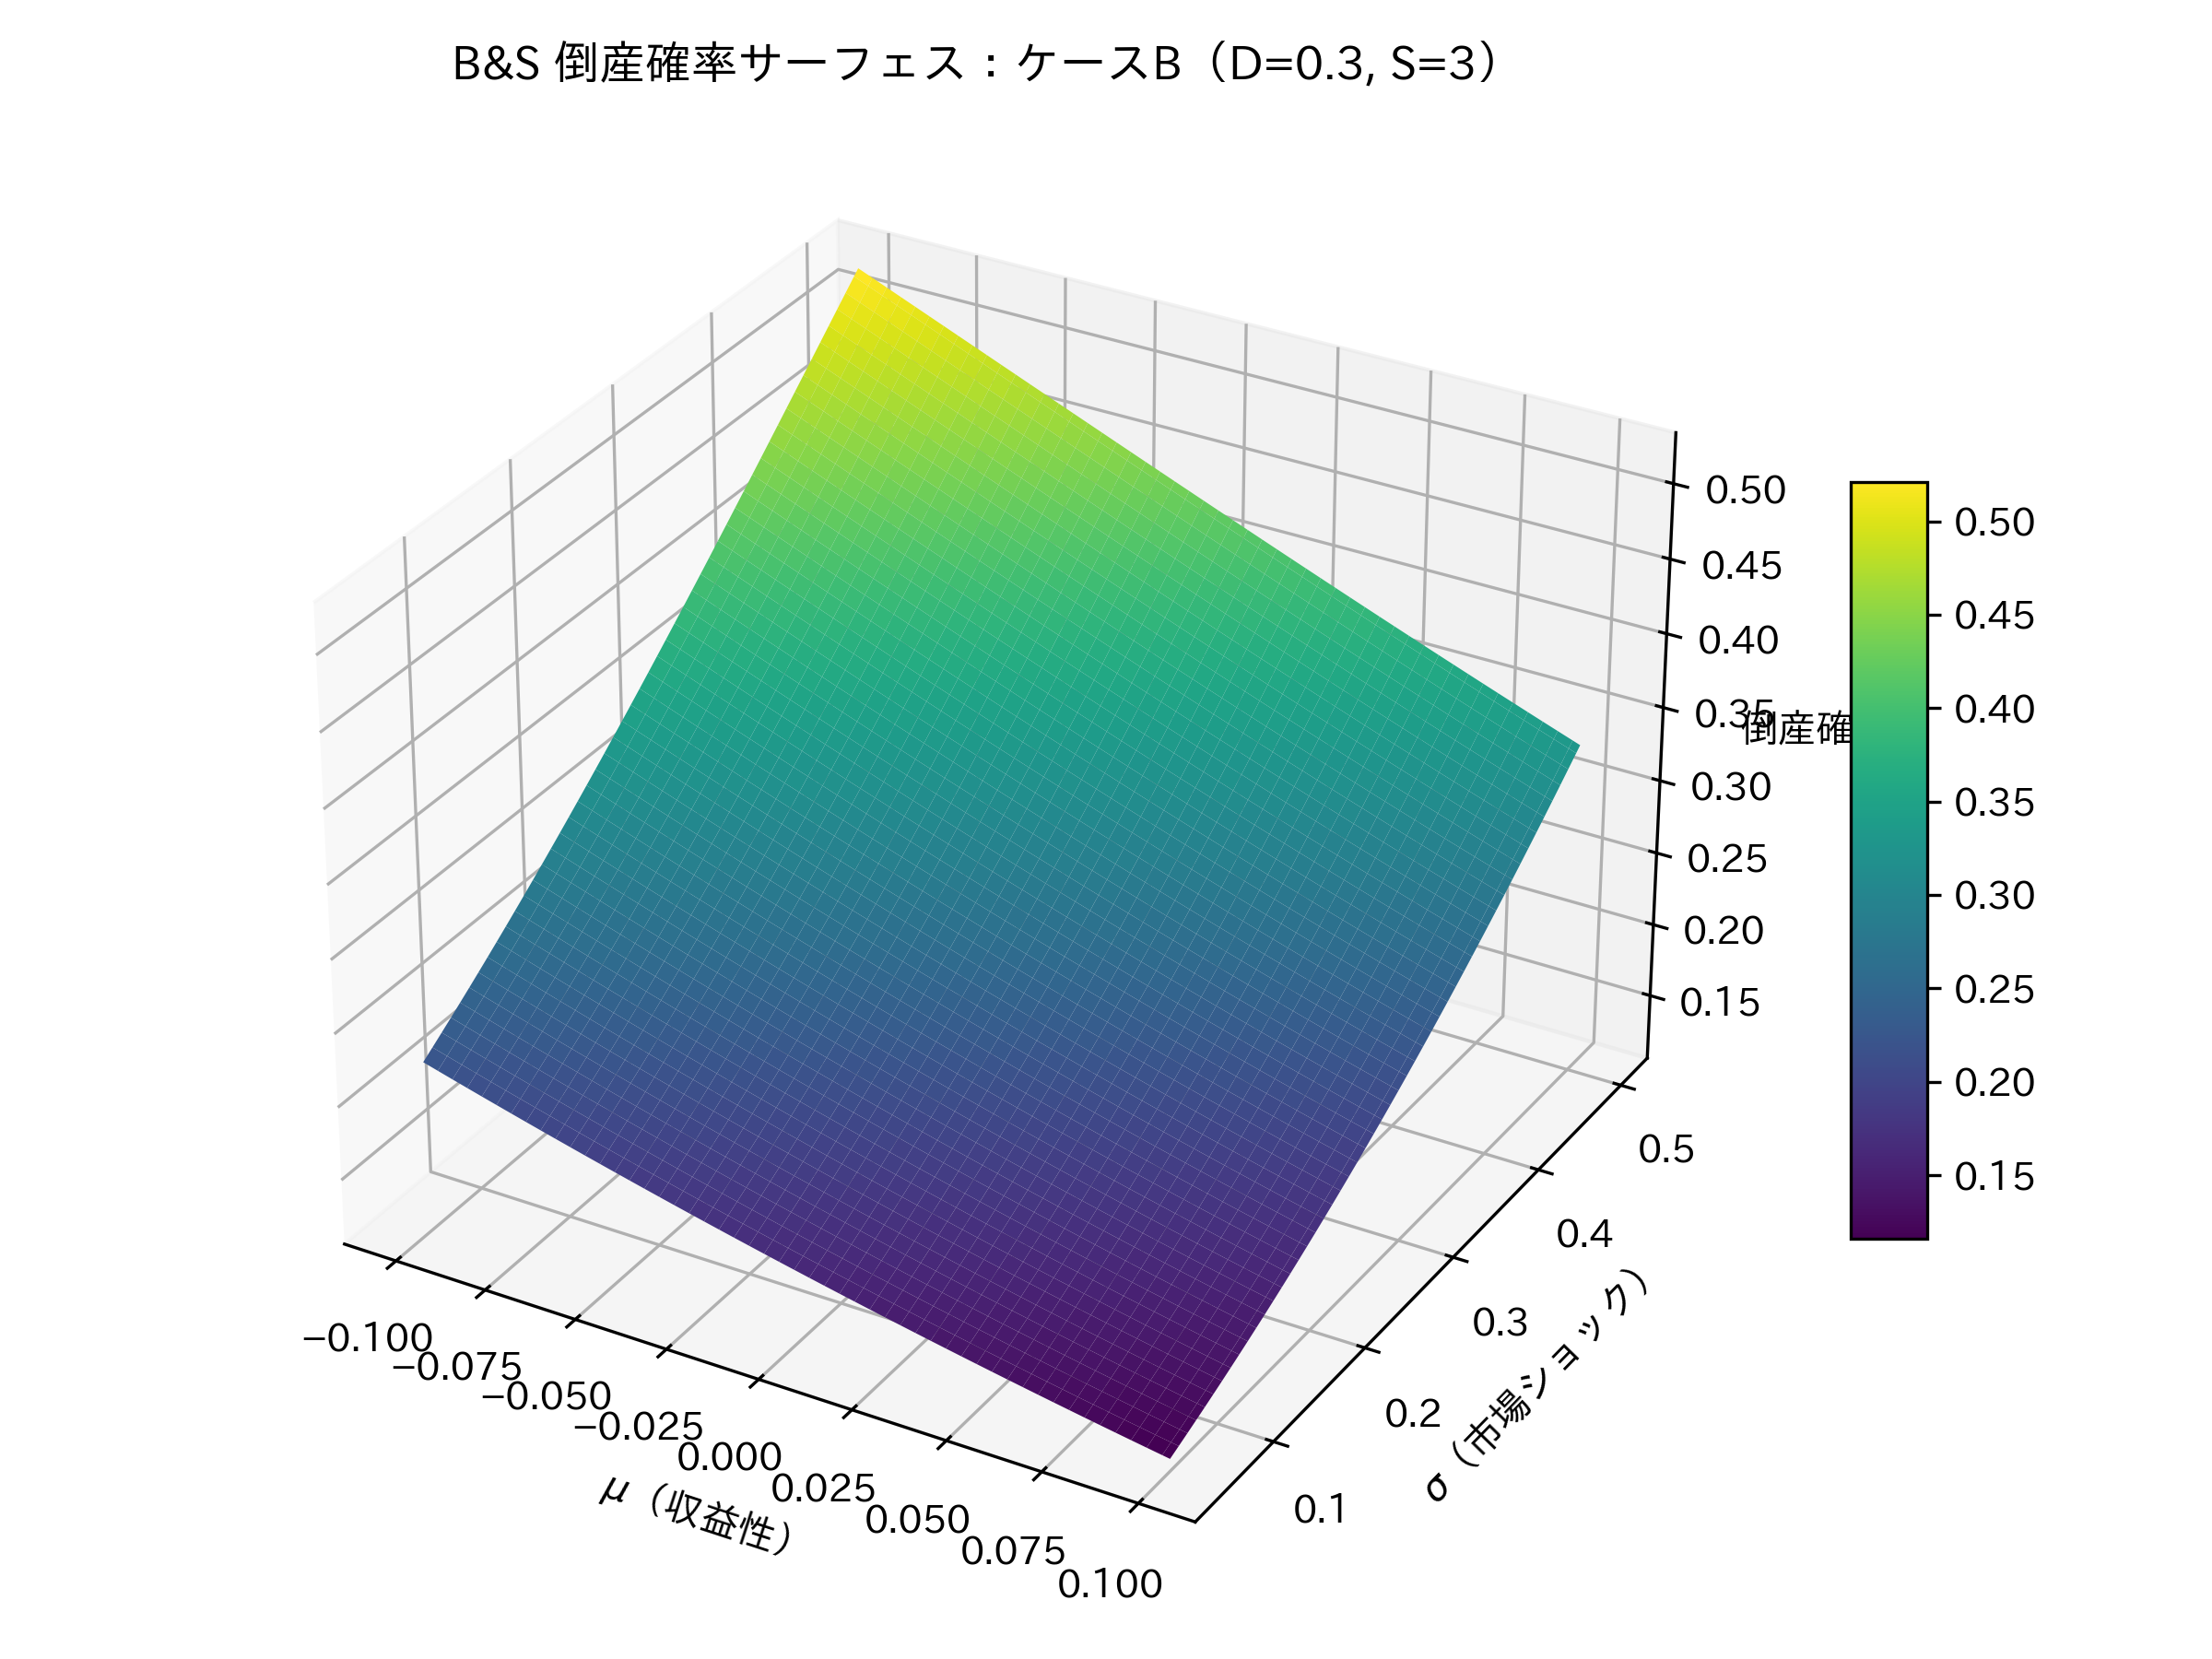
\includegraphics[width=0.75\linewidth]{figures/bs_surface_caseB.png}
    \caption{B\&S 型倒産確率サーフェス：ケースB（大手系・財務健全）}
    \label{fig:bs_surface_caseB}
\end{figure}

% ---------- ケースC ----------
\subsubsection*{ケースC：$D=0.8,\ S=0$（独立系・負債過多）}

\begin{figure}[H]
    \centering
    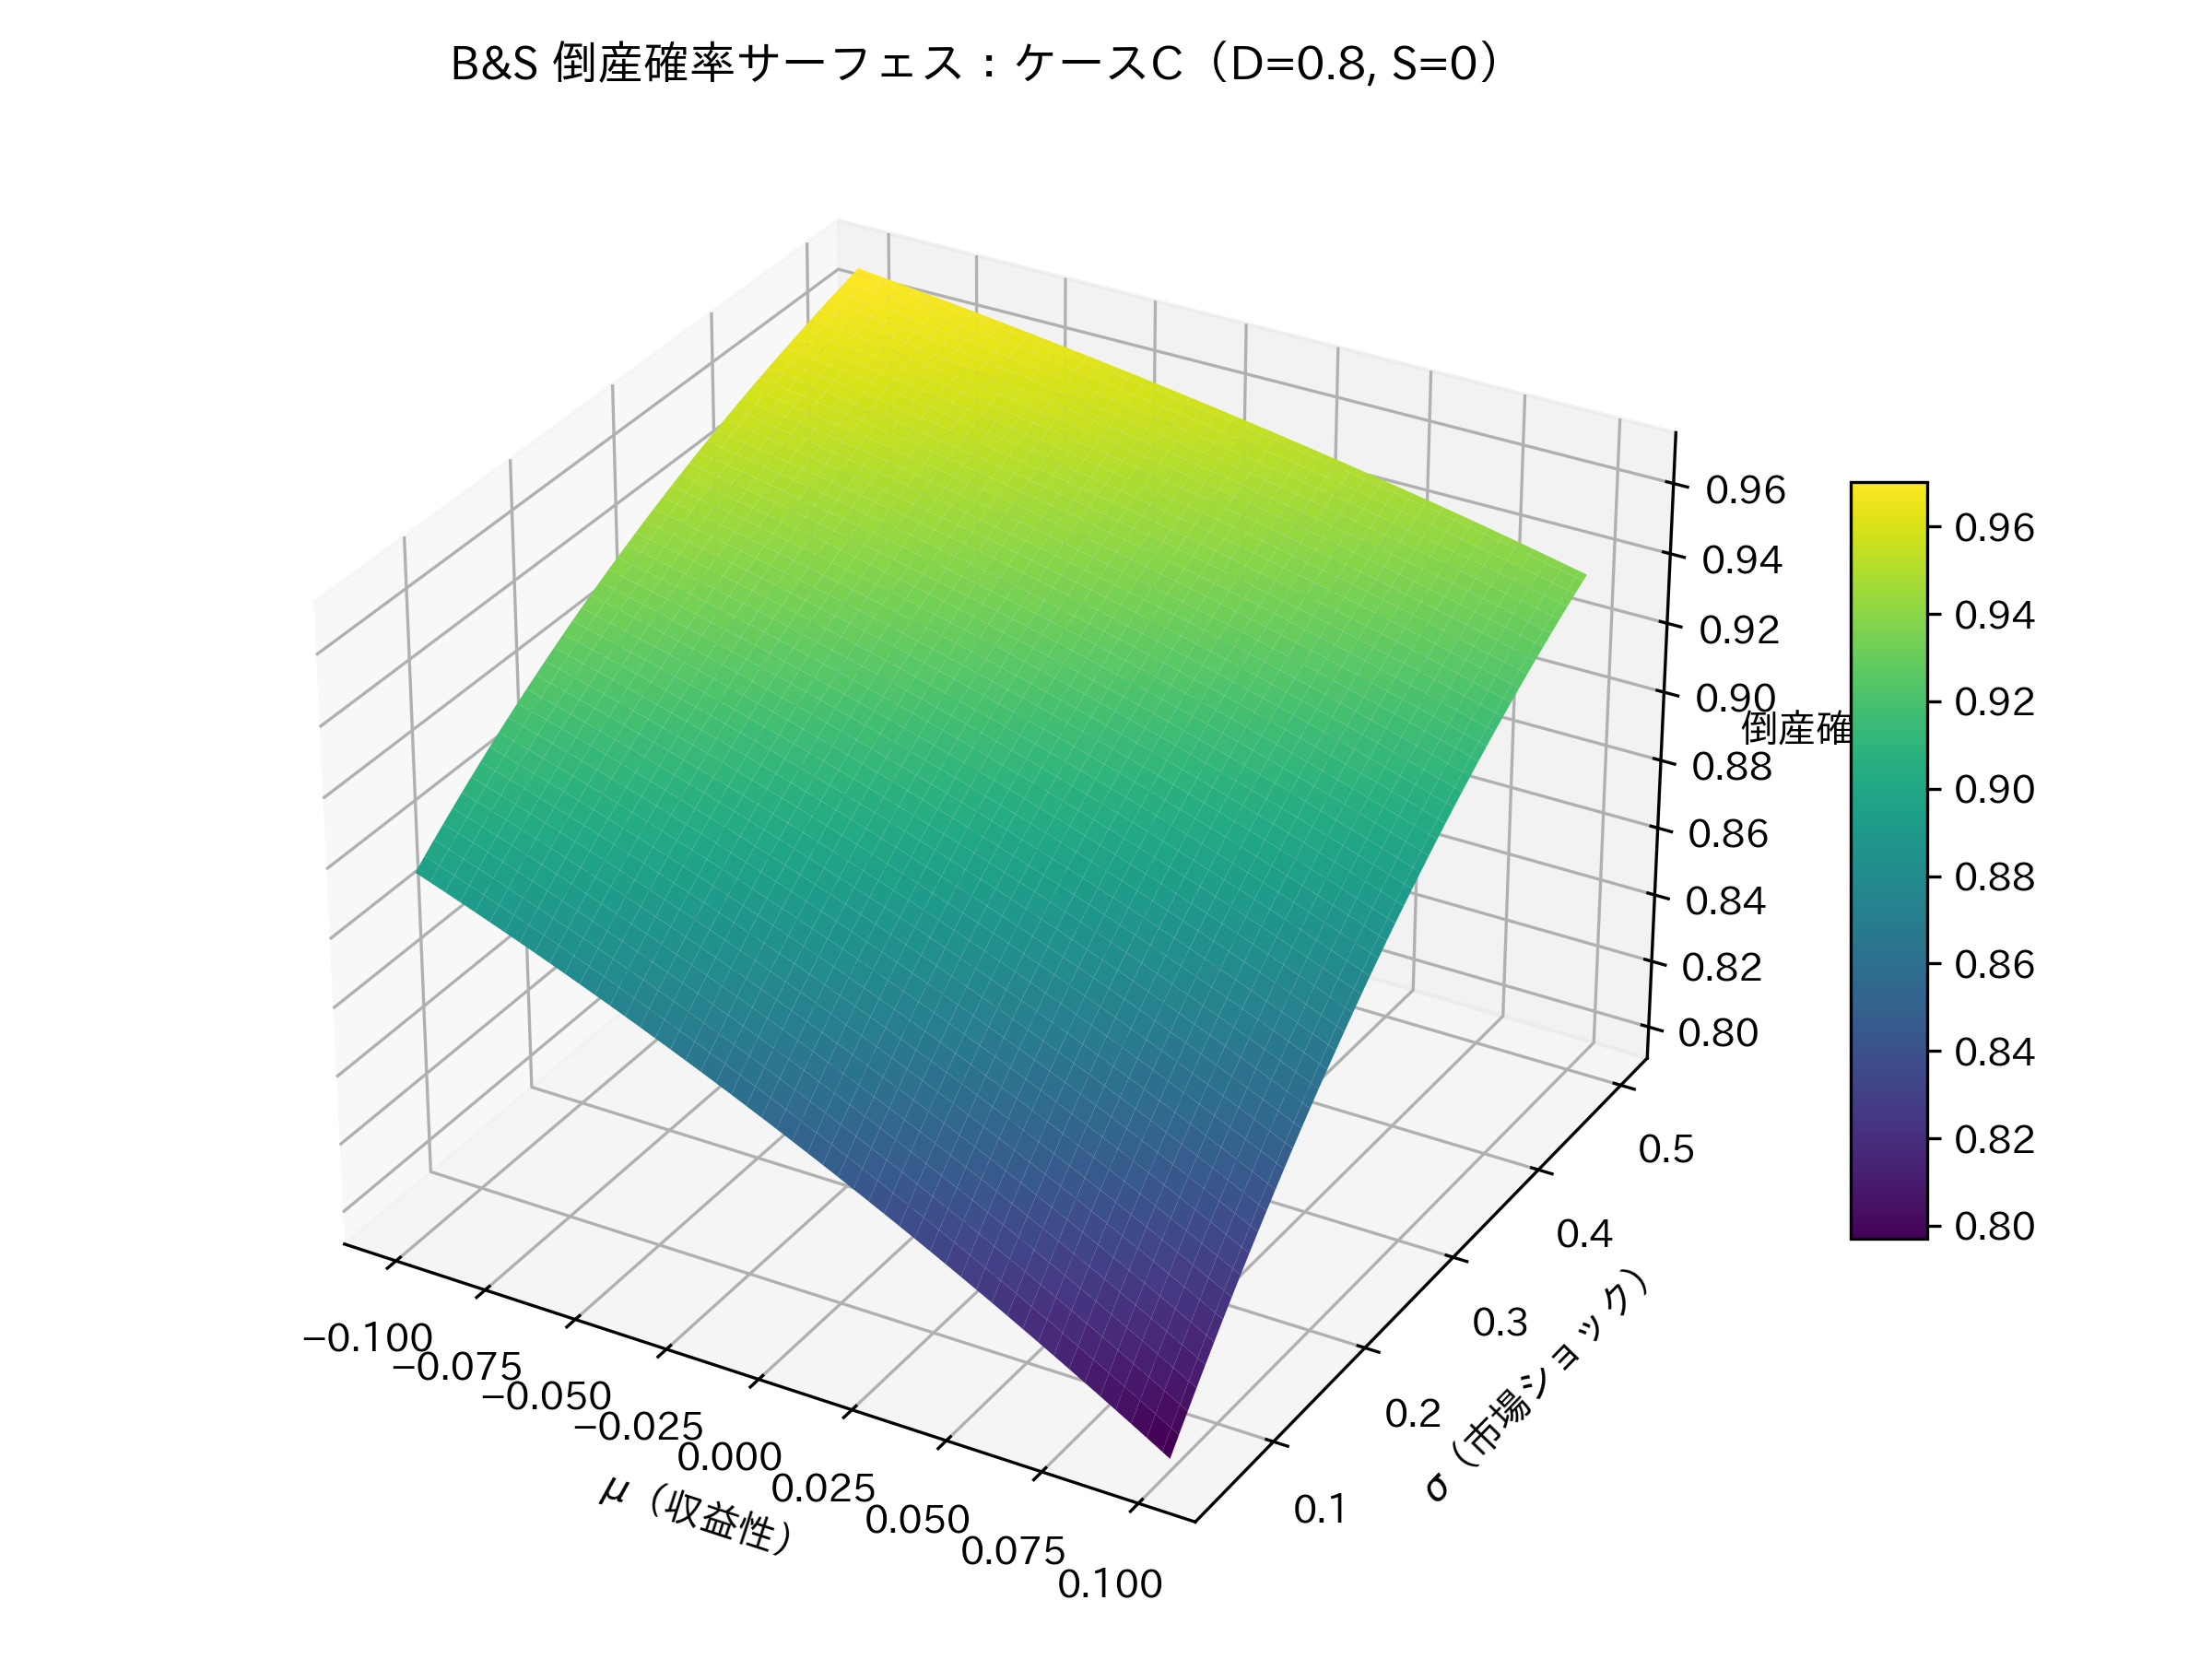
\includegraphics[width=0.75\linewidth]{figures/bs_surface_caseC.png}
    \caption{B\&S 型倒産確率サーフェス：ケースC（独立系・負債過多）}
    \label{fig:bs_surface_caseC}
\end{figure}

% ---------- ケースD ----------
\subsubsection*{ケースD：$D=0.8,\ S=3$（大手系・負債過多）}

\begin{figure}[H]
    \centering
    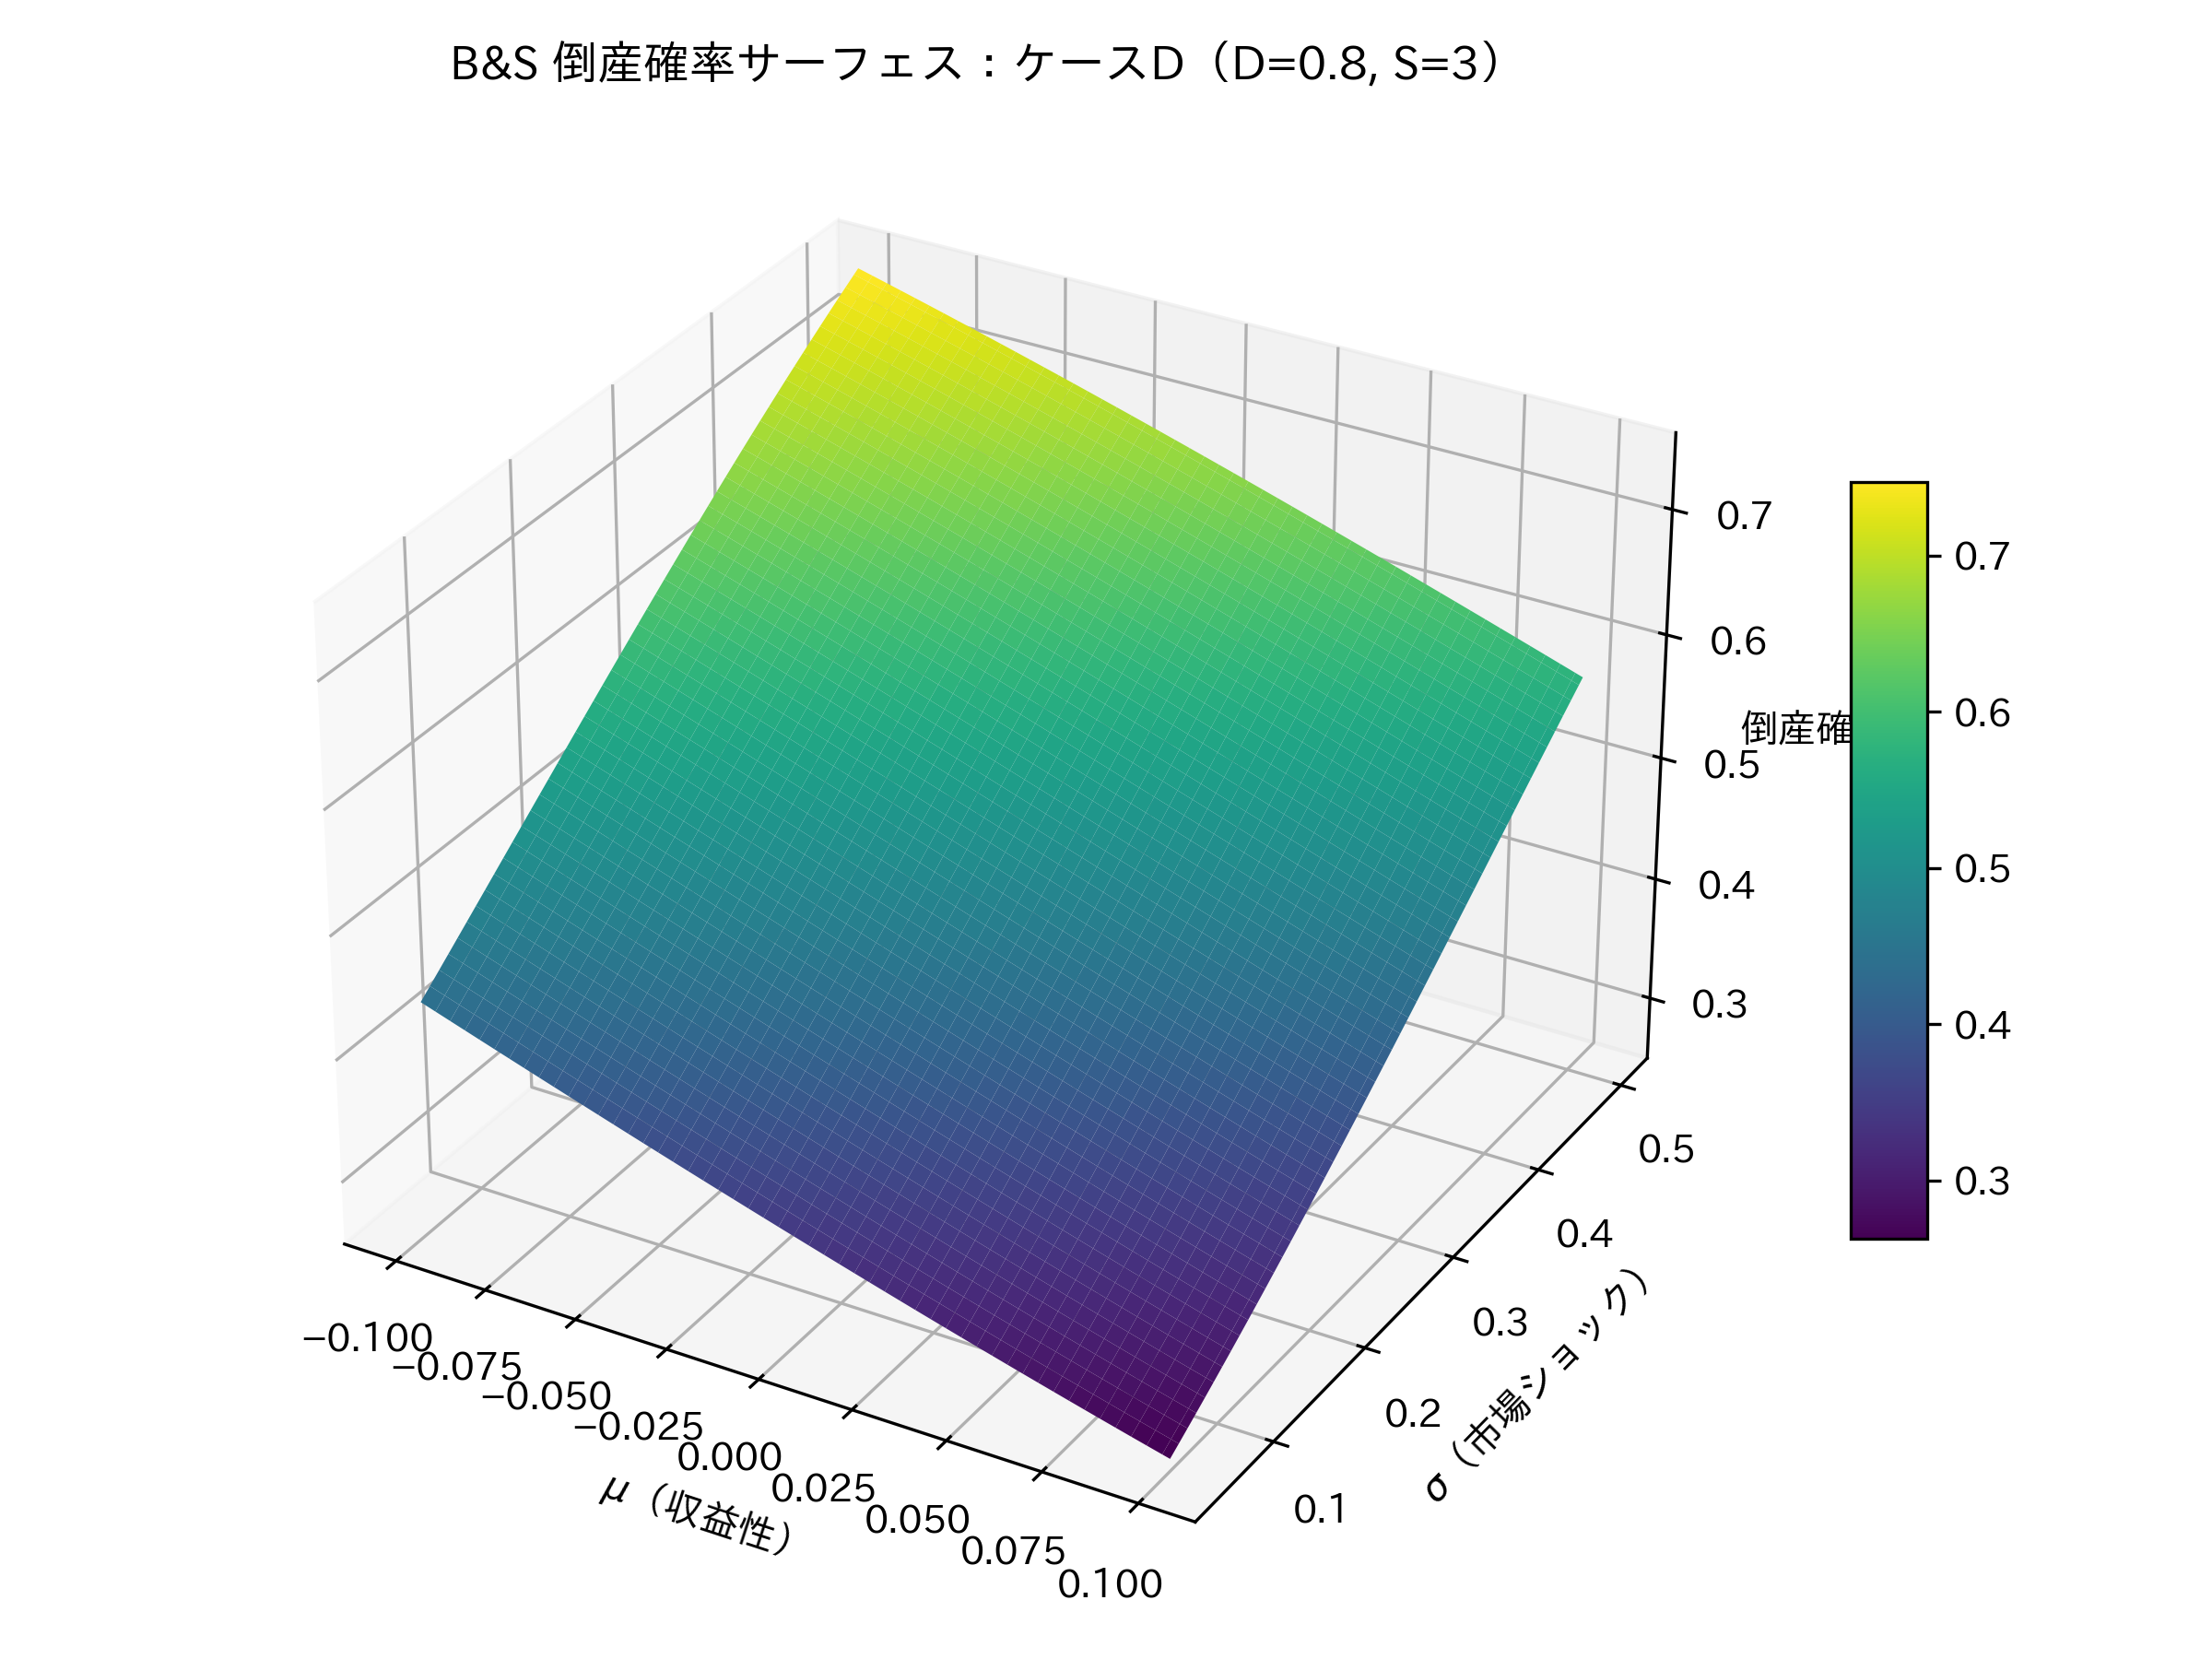
\includegraphics[width=0.75\linewidth]{figures/bs_surface_caseD.png}
    \caption{B\&S 型倒産確率サーフェス：ケースD（大手系・負債過多）}
    \label{fig:bs_surface_caseD}
\end{figure}

% ---------- ケースE ----------
\subsubsection*{ケースE：$D=0.5,\ S=1$（地域新電力）}

\begin{figure}[H]
    \centering
    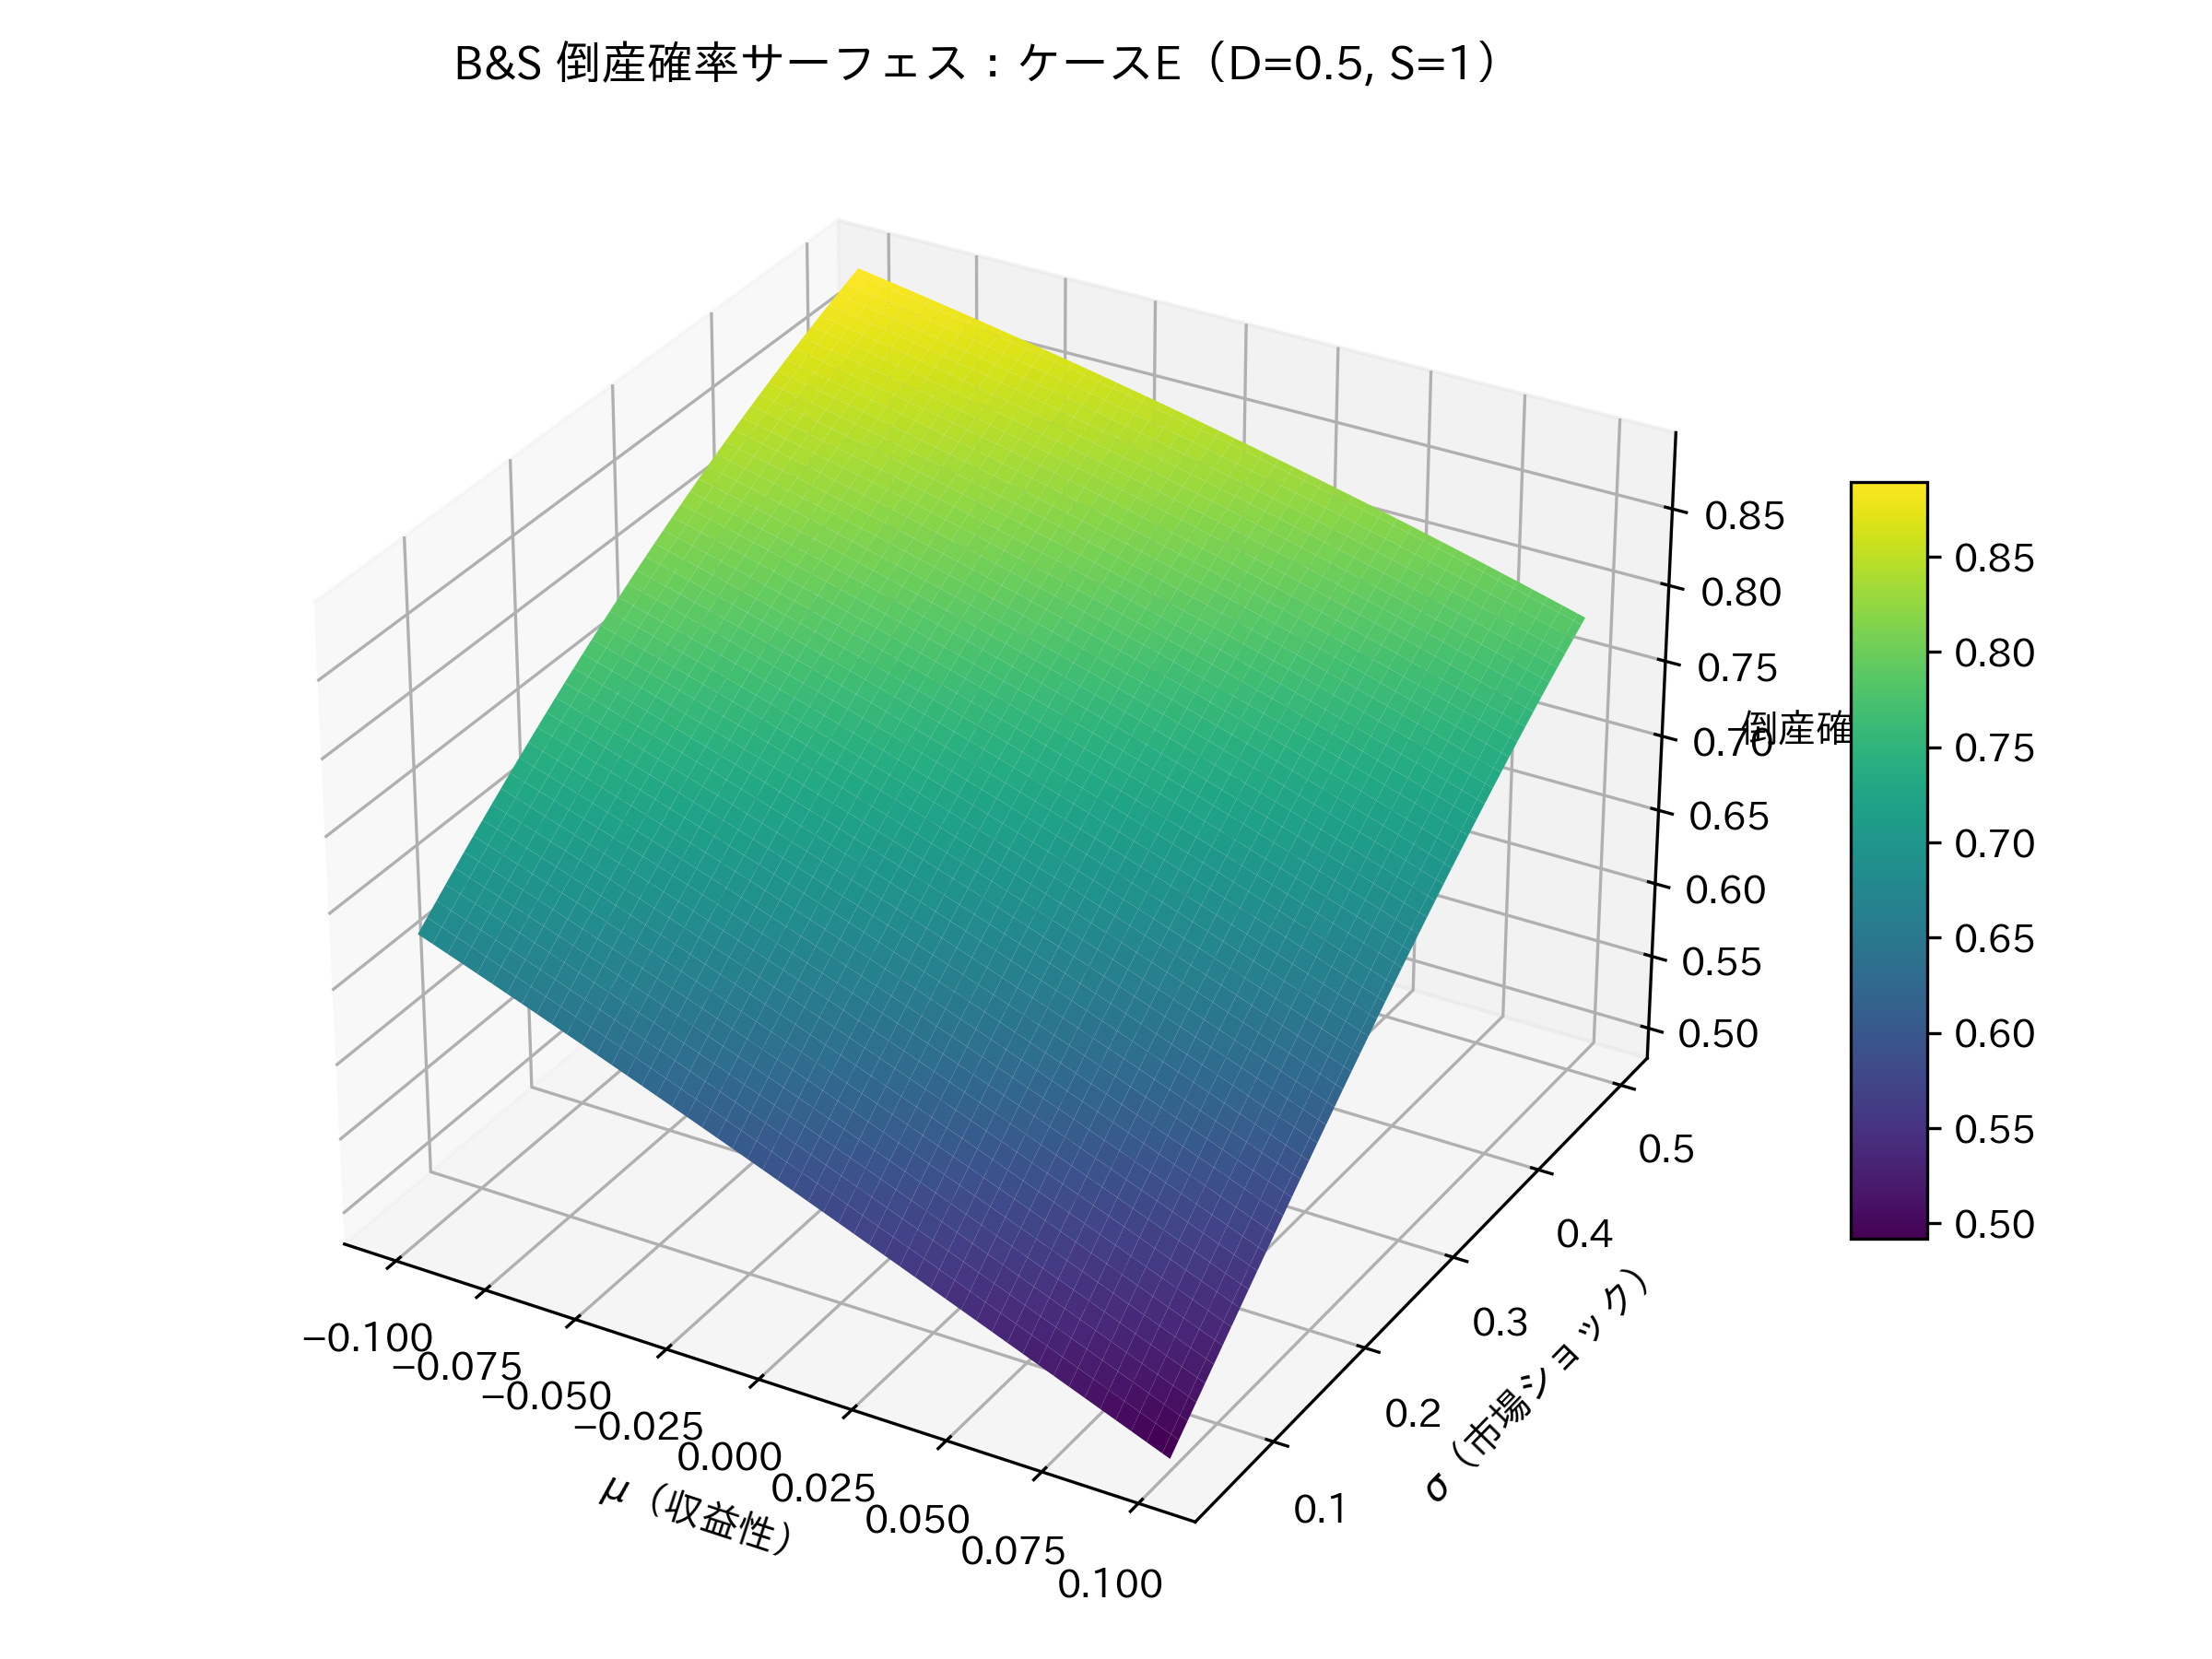
\includegraphics[width=0.75\linewidth]{figures/bs_surface_caseE.png}
    \caption{B\&S 型倒産確率サーフェス：ケースE（地域新電力）}
    \label{fig:bs_surface_caseE}
\end{figure}

% ---------- ケースF ----------
\subsubsection*{ケースF：$D=0.5,\ S=2$（商社系）}

\begin{figure}[H]
    \centering
    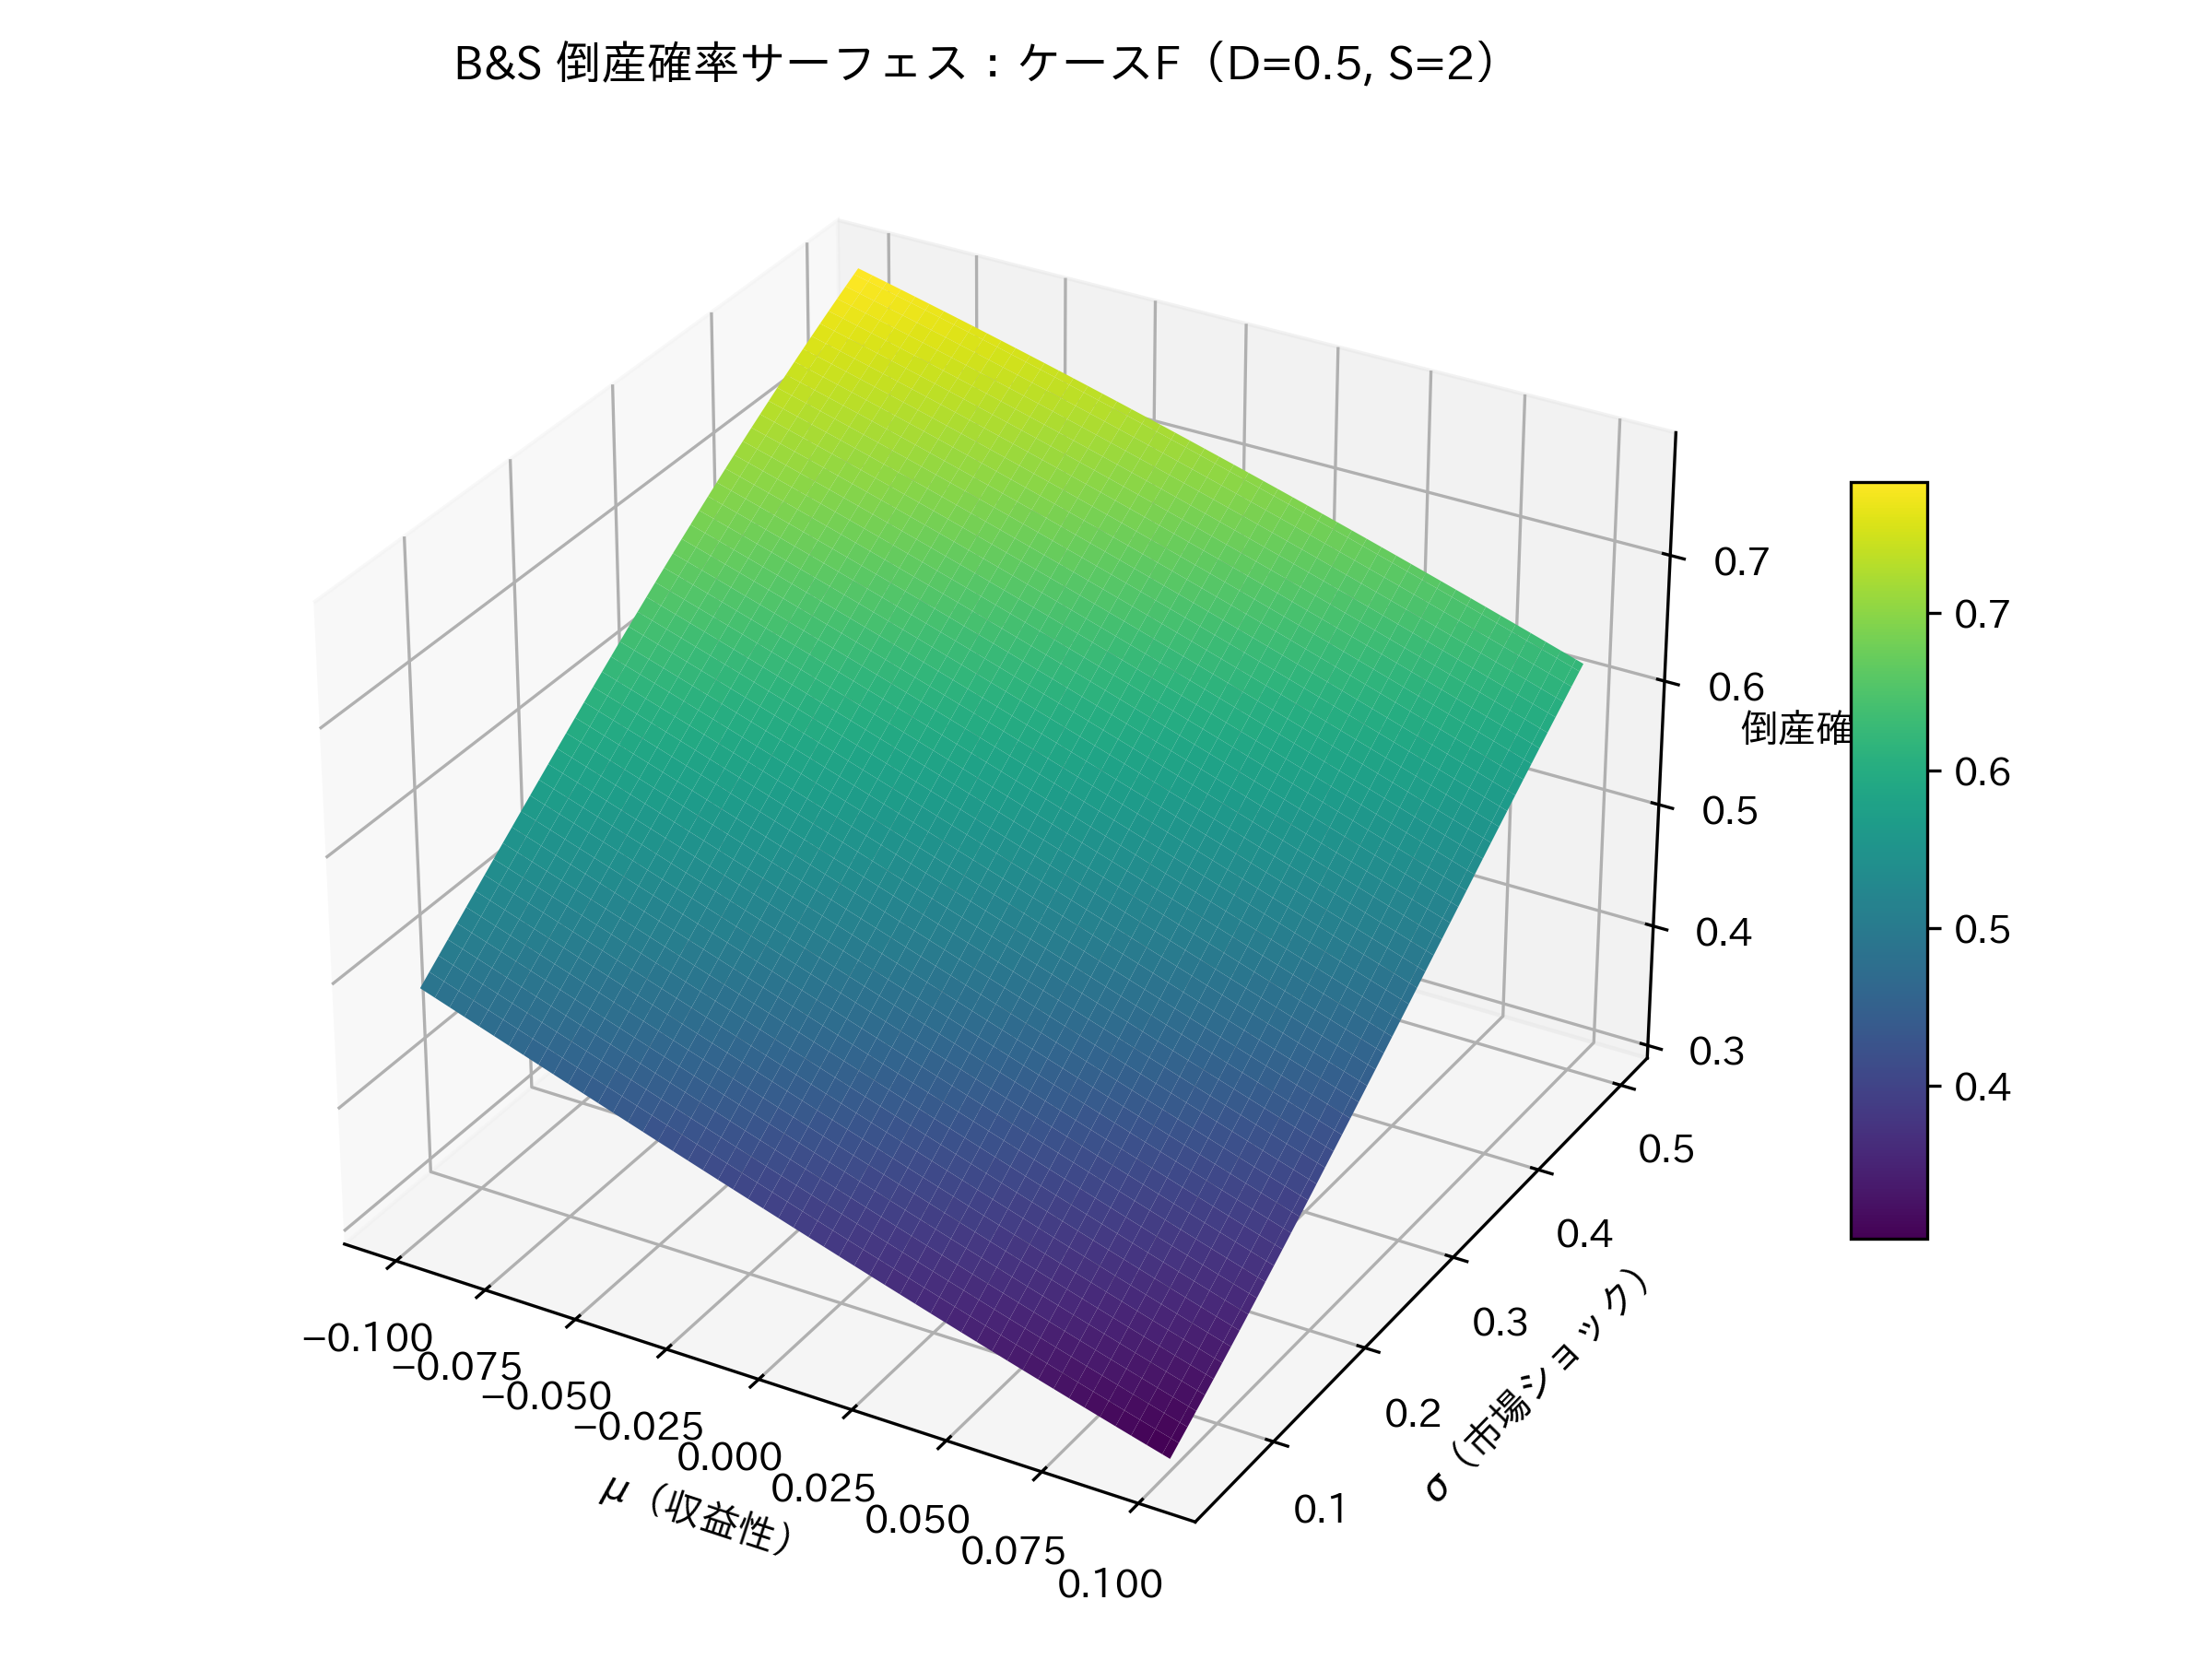
\includegraphics[width=0.75\linewidth]{figures/bs_surface_caseF.png}
    \caption{B\&S 型倒産確率サーフェス：ケースF（商社系）}
    \label{fig:bs_surface_caseF}
\end{figure}

% ------------------------------------------------------------
\subsection{Merton 型シミュレーションとの整合性}

B\&S 型ロジットモデルは企業価値プロセスを明示的に扱わない reduced-form モデルであるが，
上記のサーフェス比較から，以下の点が確認される。

\begin{itemize}
    \item $\mu$ の上昇は倒産確率を低下させる。
    \item $\sigma$ の上昇は倒産確率を上昇させる。
    \item 支援能力 $S$ が高いほど倒産確率は低下する。
    \item 負債比率 $D$ が高いほど倒産確率は急激に上昇する。
\end{itemize}

これらは第6章前半の Merton 型シミュレーションと同じ方向性を示しており，
両モデルが新電力企業の倒産リスク構造について
共通の含意を持つことを示している。

% ------------------------------------------------------------
\subsection{本節の含意と第8章への橋渡し}

本節の B\&S 型倒産リスクシミュレーションにより，
Merton 型理論モデルと B\&S 型ロジットモデルが，
新電力企業の倒産リスクを規定する主要因
（収益性 $\mu$，市場ショック $\sigma$，支援能力 $S$，負債比率 $D$）
について整合的な構造を持つことが確認された。

すなわち，B\&S 型ロジットモデルは，
Merton 型理論モデルが示す倒産確率の符号条件や相対的重要度を
現実データの枠組みで実装したものであり，
第8章で構築する潜在倒産距離モデルの妥当性を理論的に補強する役割を果たす。

さらに，本章で示した倒産確率サーフェスおよびケース間の差分サーフェスは，
新電力企業の財務構造の違いが倒産確率にどのように反映されるかを
視覚的かつ体系的に把握するためのものであり，
本研究における重要な理論的アウトプットのひとつである。

一方，\textbf{proxy 変数（A〜D）の精度が推定係数や倒産確率の識別性能に与える影響を
理想化された世界で評価する proxy 妥当性シミュレーションは，
本章の構造分析を計量的に補完するものであり，
その詳細は付録Cにまとめている}。
これにより，第8章の潜在倒産距離モデルおよび第9章の Ordered Logit 推定に先立ち，
proxy の妥当性と限界を理論的に裏付けることができる。

以上より，本章は，
\textbf{理論モデル（第4章）→ シミュレーション分析（第7章）→ 潜在倒産距離モデル（第8章）→ Ordered Logit 実証分析（第9章）}
という本研究の一連の流れの中で，
理論編と実証編を接続する重要な役割を果たす。


\chapter{実証モデルの構築：潜在倒産距離 $Z_{\text{lin}}$ とロジット推定}
\label{chap:latent_default_distance}

\section*{第7章との接続：連続モデルから潜在変数モデルへの橋渡し}

第7章では，Merton 型倒産モデルおよび Bharath \& Shumway（2008）に基づく
倒産確率の連続モデルを用いて，倒産距離 $Z_{\text{lin}}$ の構造的挙動を
シミュレーションにより可視化した。
倒産距離は連続的な指標であり，収益性 $\mu$，市場ショック感応度 $\sigma$，
負債比率 $D$ の変化に応じて滑らかに変動する。

しかし，実際の倒産データでは倒産確率そのものは観測できず，
企業は


\[
\text{stage} \in \{0,1,2\}
\]


（存続・財務悪化・倒産）という離散的な段階としてのみ観測される。
このため，連続的な倒産距離をそのまま実証分析に用いることはできない。

そこで本章では，連続的倒産距離 $Z_{\text{lin}}$ を
\textbf{潜在変数 $y^*$ として統計モデルに写像し，複数の閾値を跨ぐことで
離散的倒産ステージが生成される Ordered Logit モデル}を構築する。
すなわち，

\begin{itemize}
    \item 第7章：連続的倒産距離の構造を理論的に理解する段階
    \item 第8章：連続的倒産距離を潜在変数モデルへと写像する段階
    \item 第9章：潜在変数が閾値を跨ぐことで離散的倒産ステージを推定する段階
\end{itemize}

という三段階構造により，理論モデルと実証モデルを統合する。

本章は，連続モデル（第7章）と離散モデル（第9章）の間を接続する
「橋渡し」の役割を果たし，倒産距離の構造を実証的に推定可能な形へと
定式化するものである。

\subsection*{連続モデルと離散モデルの対応関係の整理}

第7章では，倒産距離 $Z_{\text{lin}}$ を用いた連続的倒産確率モデルをシミュレーションにより可視化し，
収益性 $\mu$，市場ショック感応度 $\sigma$，負債比率 $D$ の変化が倒産確率に与える影響を体系的に確認した。
これに対し，第9章では，倒産が


\[
\text{stage} \in \{0,1,2\}
\]


という離散的な段階として観測されることを踏まえ，Ordered Logit モデルを用いて倒産ステージの発生確率を推定する。

すなわち，本研究は
\begin{itemize}
    \item 第7章：倒産確率を連続的に扱う理論モデルの挙動を理解する段階
    \item 第8章：連続的倒産距離を潜在変数 $y^*$ に写像する統計モデルを構築する段階
    \item 第9章：潜在変数が閾値を跨ぐことで離散的倒産ステージを推定する段階
\end{itemize}
という三段階構造を採用している。

この構造は Ordered Logit モデルの本質（連続的潜在変数と複数の閾値）と完全に整合しており，
連続モデルと離散モデルの間に不整合は存在しない。
むしろ，連続モデルで確認された倒産距離の構造的特徴が，
離散モデルの推定結果（係数符号・cutpoint）にどのように反映されるかを理解するための基盤となる。

以下の表では，本研究における連続モデル（第7章）と離散モデル（第9章）の対応関係を体系的に整理し，
両者の役割分担と整合性を視覚的に示す。

\begin{table}[H]
\centering
\caption{連続モデル（第7章）と離散モデル（第9章）の対応関係}
\label{tab:continuous_discrete_mapping}
\begin{tabular}{p{4cm} p{5cm} p{6cm}}
\toprule
\textbf{概念} & \textbf{連続モデル（第7章）} & \textbf{離散モデル（第9章）} \\
\midrule

倒産リスクの扱い &
倒産距離 $Z_{\text{lin}}$ に基づく連続的倒産確率


\[
p = \Lambda(-Z_{\text{lin}})
\]


&
潜在変数 $y^*$ が閾値を跨ぐことで離散的ステージが生成


\[
\text{stage} \in \{0,1,2\}
\]

 \\

モデルの性質 &
連続的に変化する倒産確率（滑らかなリスク指標） &
離散的に観測される倒産段階（存続・財務悪化・倒産） \\

変数の役割 &
$\mu$，$\sigma$，$D$ が倒産距離を直接押し上げ／押し下げる &
$\mu$，$\sigma$，$D$ が潜在変数 $y^*$ を通じてステージ遷移確率を規定 \\

閾値の扱い &
閾値は設定しない（連続モデルのため） &
閾値 $\tau_1, \tau_2$ をデータから推定（Ordered Logit の本質） \\

目的 &
倒産距離の構造的挙動を理論的に理解する &
倒産ステージの発生確率を実証的に推定する \\

本研究における位置づけ &
理論モデルの挙動を可視化し、実証分析の心構えを形成する章 &
実データに基づき倒産ステージを推定する本丸の実証分析 \\

整合性 &
符号構造・相対的重要度は第9章の推定結果と一致 &
第7章の連続モデルの挙動が第9章の離散モデルの推定結果に反映される \\

\bottomrule
\end{tabular}
\end{table}


\section{本章の目的}

本章では，第4章で導出した線形倒産距離 $Z_{\text{lin}}$ を，
実証モデルとしてどのように推定可能な形へと写像するかを整理する。
すなわち，理論モデル（連続的倒産距離）と統計モデル（ロジット推定）の
橋渡しを行い，第9章の Ordered Logit 推定へと接続する役割を果たす。

本章の目的は以下の三点である。

\begin{enumerate}
    \item 線形倒産距離 $Z_{\text{lin}}$ の再掲と構造的意味の整理
    \item ロジットモデル（Logit）の定式化と拡張（相互作用項の導入）
    \item 理論的符号条件および識別の考え方の提示
\end{enumerate}

これにより，第9章で実施する Ordered Logit 推定の前段階として，
潜在倒産距離の構造を統計モデルへと写像するための基盤を整える。

% ============================================================
% 8.2 潜在倒産距離 Z_lin の再掲
% ============================================================

\section{潜在倒産距離 $Z_{\text{lin}}$ の再掲}

第4章で導出した線形倒産距離 $Z_{\text{lin}}$ は以下の構造を持つ。



\[
Z_{\text{lin}}
= a\mu - b\sigma + cS - dD,
\]



ここで，

\begin{itemize}
    \item $\mu$：企業価値の期待成長率（収益性）
    \item $\sigma$：市場ショック感応度（ボラティリティ）
    \item $S$：支援能力（親会社の財務余力）
    \item $D$：負債比率（倒産閾値の代理変数）
\end{itemize}

である。

この構造は Merton モデルの倒産距離



\[
DD = \frac{\ln(V/Thr) + (\mu - \tfrac{1}{2}\sigma^2)T}{\sigma\sqrt{T}}
\]



の一次近似として解釈できる。

本研究では，非上場企業である新電力企業のデータ制約を踏まえ，
$Z_{\text{lin}}$ を実証的に推定可能な proxy へと写像する。

% ============================================================
% 8.3 ロジットモデルの定式化
% ============================================================

\section{ロジットモデルの定式化}

倒産を二値で扱う場合，ロジットモデルは以下のように定式化される。



\[
\Pr(\text{Default}_{i,t}=1)
=
\Lambda(\alpha + \beta_1 D_{i,t} + \beta_2 \mu_{i,t} + \beta_3 \sigma_t + \beta_4 S_i),
\]



ここで $\Lambda(z)=1/(1+e^{-z})$ はロジスティック関数である。

しかし，新電力企業では倒産企業が極端に少なく，
二値ロジットでは完全分離（perfect separation）が発生する。

そのため，本研究ではロジットモデルを「潜在倒産距離の推定式」として位置づけ，
その構造を Ordered Logit の潜在変数モデルへと接続する。

% ============================================================
% 8.4 相互作用項を導入した拡張ロジットモデル
% ============================================================

\section{相互作用項を導入した拡張ロジットモデル}

新電力企業の倒産構造は，単一の財務指標ではなく，
複数のリスク要因が同時に悪化する「multiplicative」な構造を持つ。

そのため，以下のような相互作用項を含む拡張ロジットモデルを考える。



\[
\Pr(\text{Default}_{i,t}=1)
=
\Lambda(
\alpha
+ \beta_1 D_{i,t}
+ \beta_2 \mu_{i,t}
+ \beta_3 \sigma_t
+ \beta_4 (D_{i,t}\cdot\sigma_t)
+ \beta_5 (D_{i,t}\cdot\mu_{i,t})
).
\]



ここで，

\begin{itemize}
    \item $D \cdot \sigma$：負債依存度と市場ショックの同時悪化
    \item $D \cdot \mu$：負債依存度と収益性低下の同時悪化
\end{itemize}

を表す。

新電力企業では，市場ショックと負債比率が同時に悪化するケースが多く，
この相互作用項は倒産距離の multiplicative 構造を反映する。

ただし，二値ロジットでは完全分離が発生するため，
この拡張ロジットモデルは「構造的理解」のために提示するものであり，
実際の推定は第9章の Ordered Logit によって行う。

% ============================================================
% 8.5 理論的符号条件
% ============================================================

\section{理論的符号条件}

本節では，潜在倒産距離モデルにおける係数の符号条件を理論的に整理する。
これらの符号条件は，第4章で導出した倒産距離 $Z_{\text{lin}}$ の構造，
および第7章で確認したシミュレーション結果と整合的であり，
第9章で推定する Ordered Logit モデルの係数解釈における基盤となる。

倒産距離の線形近似は以下で与えられる。



\[
Z_{\text{lin}} = a\mu - b\sigma + cS - dD,
\]



ここで，$Z_{\text{lin}}$ が大きいほど企業は安全側に位置し，
$Z_{\text{lin}}$ が小さいほど倒産側に近づく。
したがって，倒産確率は



\[
p = \Lambda(-Z_{\text{lin}})
\]



のように $Z_{\text{lin}}$ の減少に伴って上昇する。

この構造から，潜在変数モデルにおける係数の符号条件は以下のように導かれる。

\begin{itemize}
    \item $\beta_1 > 0$：負債比率 $D$ が高いほど倒産距離は低下し，倒産確率は上昇する  
    （負債依存度の増大は財務柔軟性を低下させ，ショック耐性を弱める）

    \item $\beta_2 < 0$：収益性 $\mu$ が高いほど倒産距離は上昇し，倒産確率は低下する  
    （資産成長率の高さは内部資金の蓄積とショック吸収力の向上を意味する）

    \item $\beta_3 > 0$：市場ショック感応度 $\sigma$ が大きいほど倒産距離は低下し，倒産確率は上昇する  
    （価格変動の大きさはキャッシュフローの不確実性を増幅し，倒産閾値への接近を促す）

    \item $\beta_4 > 0$：負債比率と市場ショックの同時悪化は倒産確率を増幅する  
    （multiplicative な倒産構造により，$D$ と $\sigma$ の相互作用は単独の効果以上の影響を持つ）
\end{itemize}

これらの符号条件は，第4章で示した倒産距離 $Z_{\text{lin}}$ の構造と整合的であるだけでなく，
第7章のシミュレーションにおいても視覚的に確認された。
具体的には，

\begin{itemize}
    \item $\mu$ の上昇は倒産確率サーフェスを大きく押し下げる（安全側へ移動）
    \item $\sigma$ の上昇は倒産確率を急激に押し上げる（危険側へ移動）
    \item $D$ の上昇は倒産確率を体系的に増加させる
    \item $D \times \sigma$ の同時悪化は倒産確率の増加を非線形に加速させる
\end{itemize}

という挙動が確認されており，理論モデルとシミュレーション結果が一致している。

さらに，第9章の Ordered Logit 推定においても，
これらの符号条件は実証的に支持される。
すなわち，

\begin{itemize}
    \item $\beta_1$（負債比率）は正  
    \item $\beta_2$（収益性）は負  
    \item $\beta_3$（市場ショック感応度）は正  
\end{itemize}

という符号構造が推定結果として得られ，
理論モデル → シミュレーション → 実証分析の三段階が一貫した構造を形成している。

以上より，本節で示した符号条件は，
潜在倒産距離モデルの理論的妥当性を裏付けるとともに，
第9章の Ordered Logit 推定における係数解釈の基礎となる。

\begin{figure}[H]
    \centering
    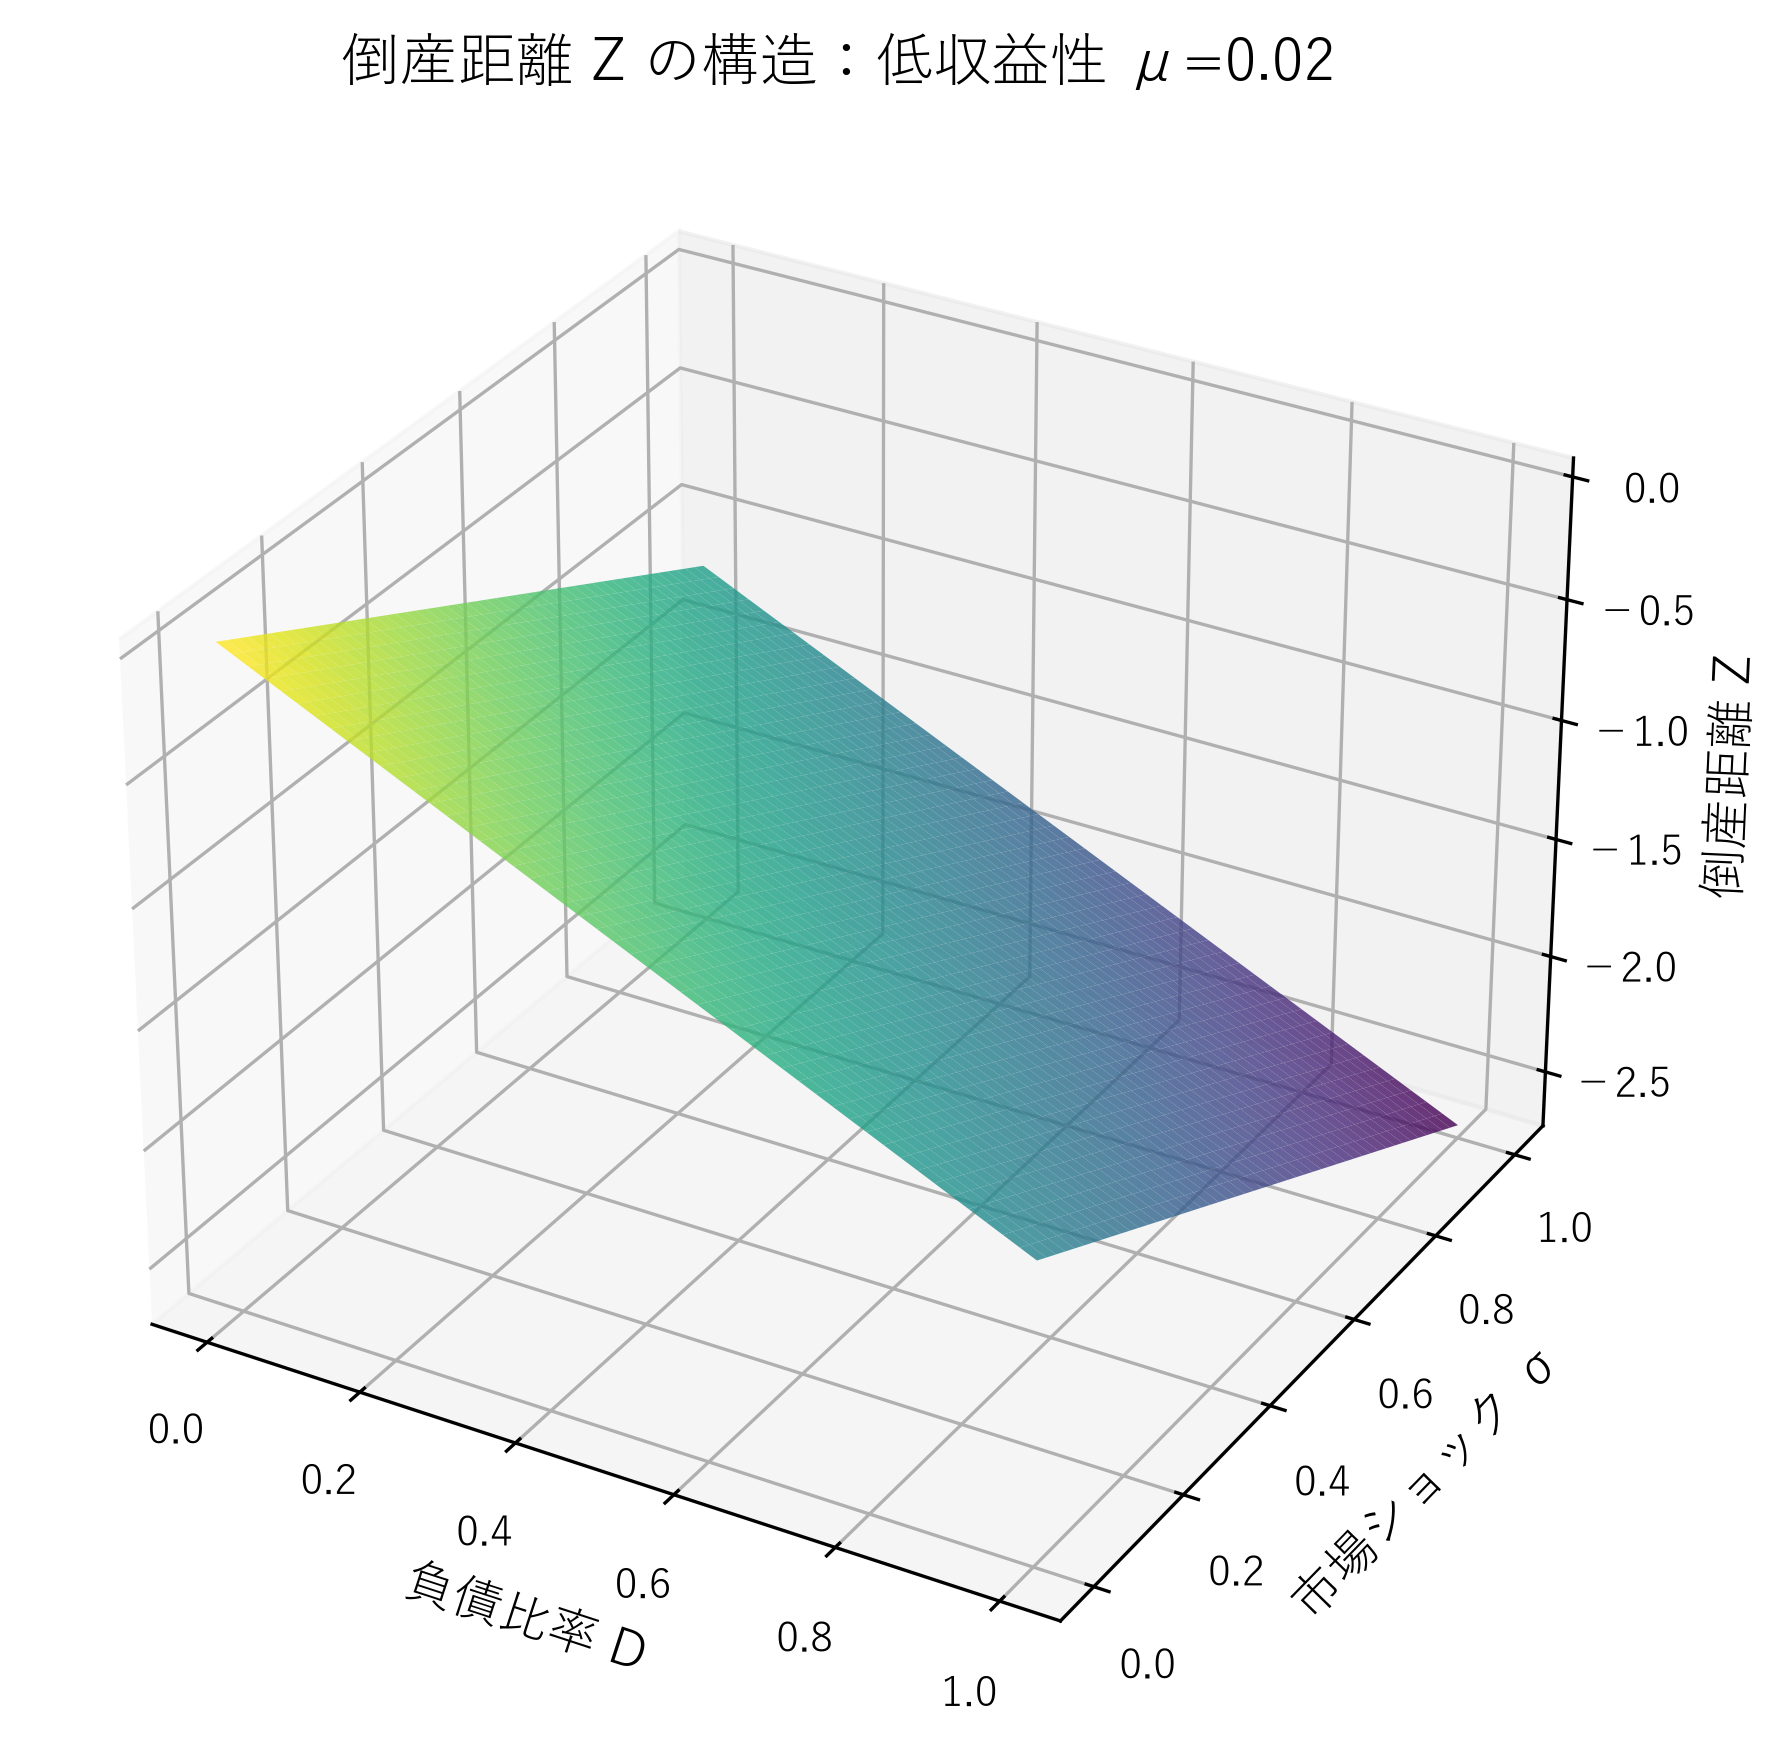
\includegraphics[width=0.85\textwidth]{Python/figures/sign_surface_0.02.png}
    \caption{倒産距離 $Z_{\text{lin}}$ の3D構造：低収益性（$\mu=0.02$）}
    \label{fig:surface_mu_002}
\end{figure}

\begin{figure}[H]
    \centering
    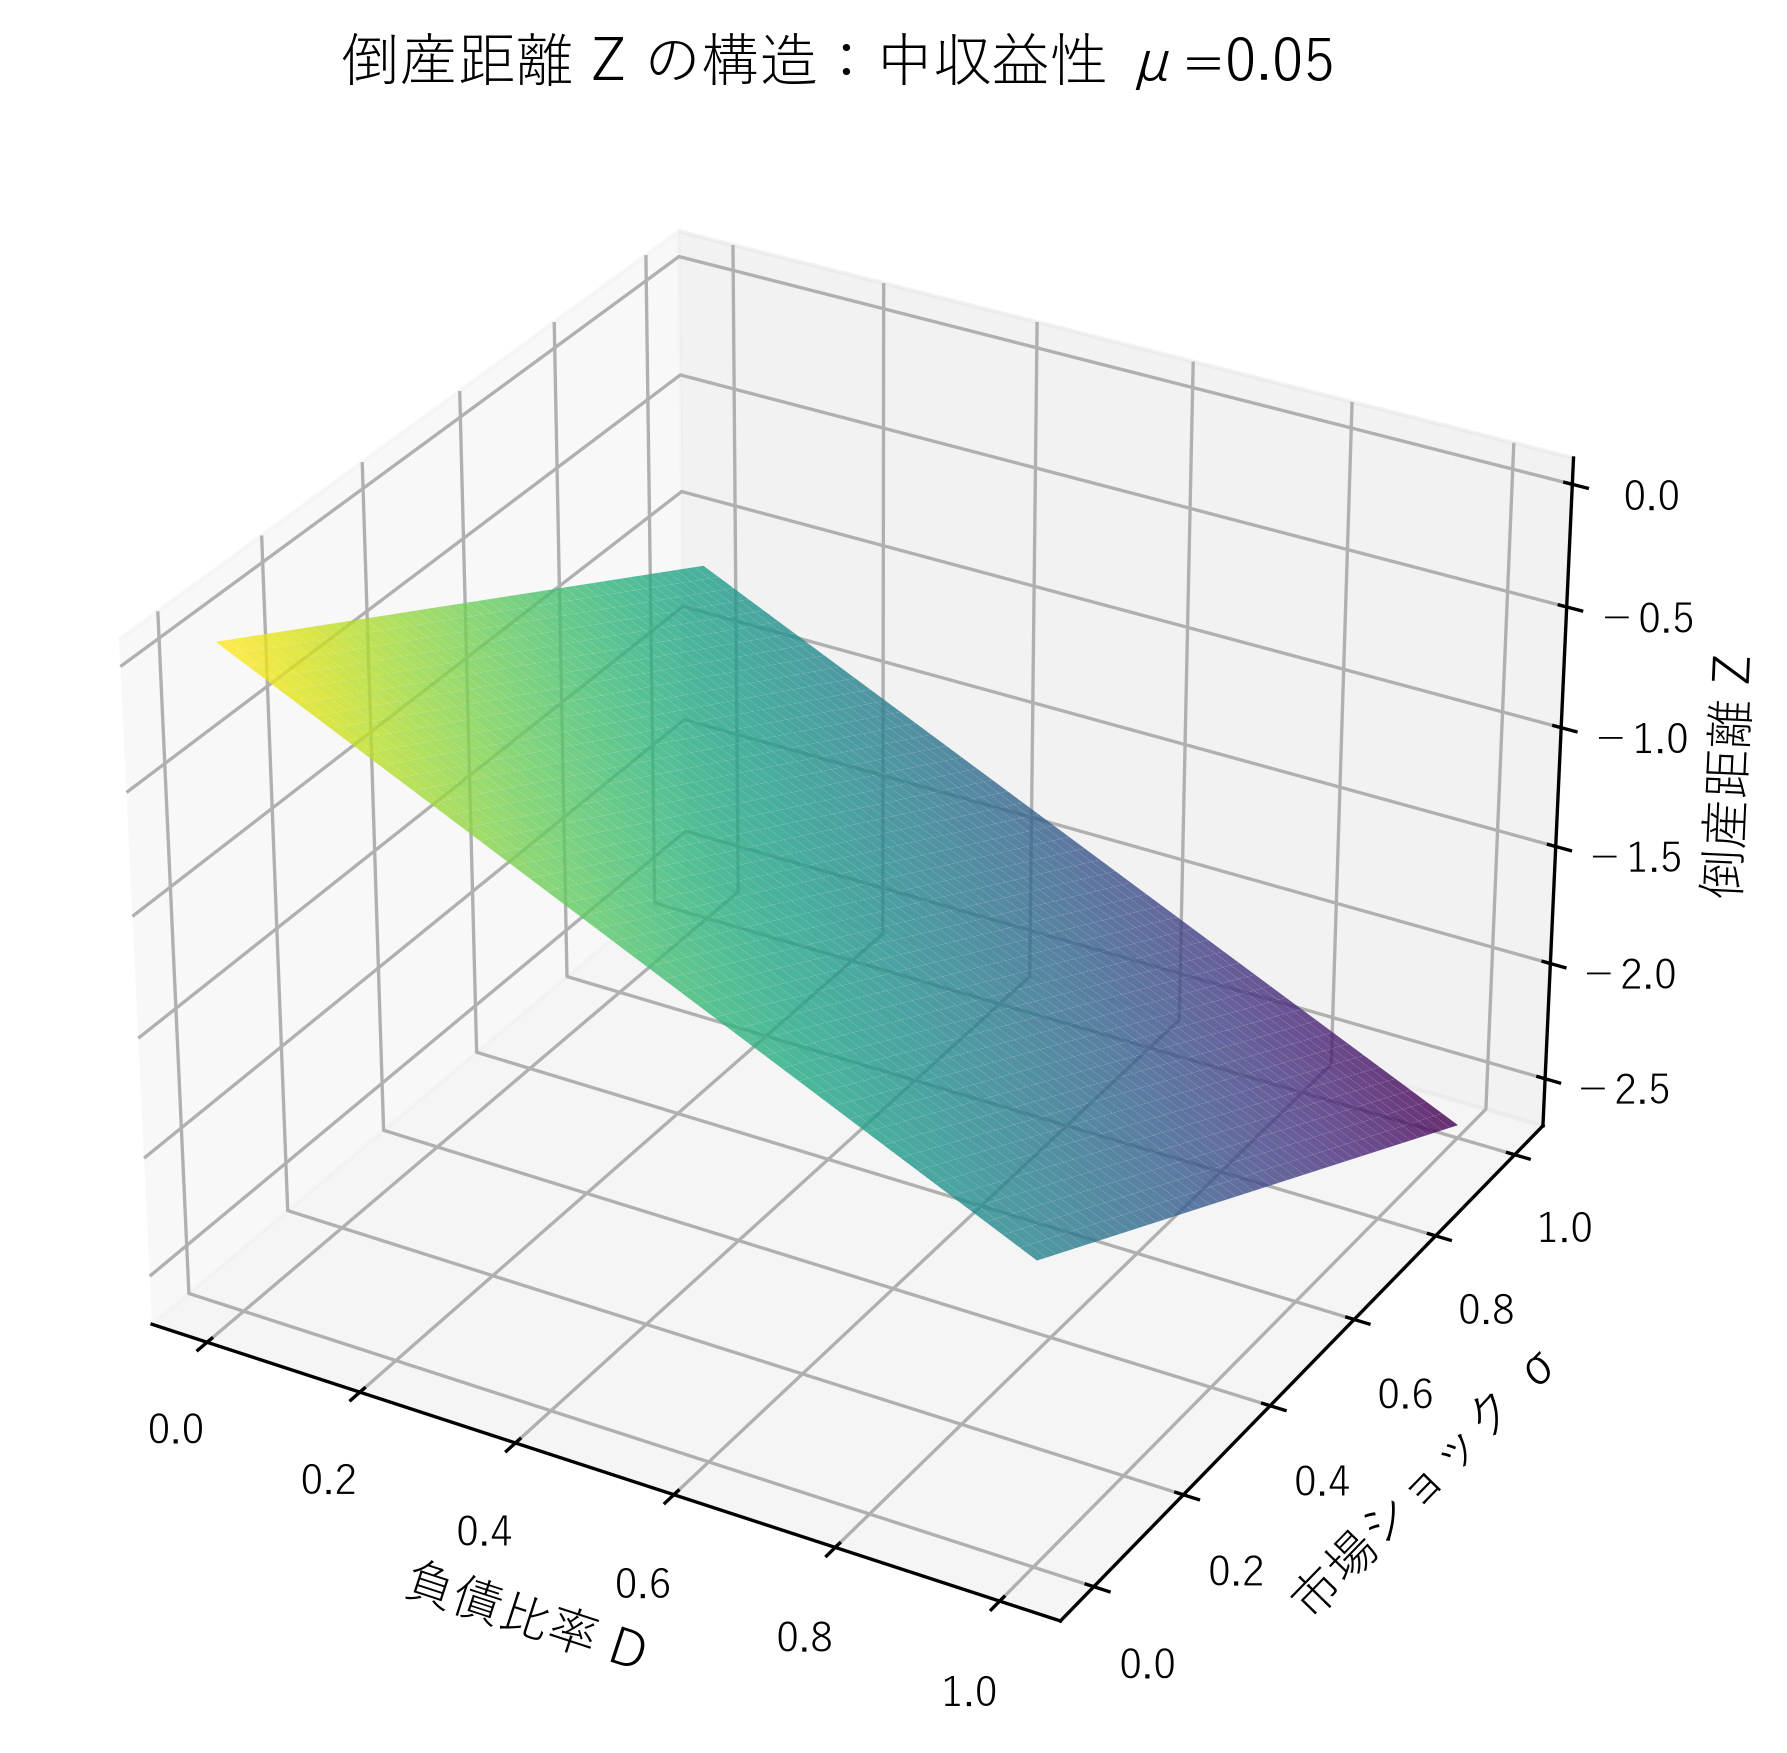
\includegraphics[width=0.85\textwidth]{Python/figures/sign_surface_0.05.png}
    \caption{倒産距離 $Z_{\text{lin}}$ の3D構造：中収益性（$\mu=0.05$）}
    \label{fig:surface_mu_005}
\end{figure}

\begin{figure}[H]
    \centering
    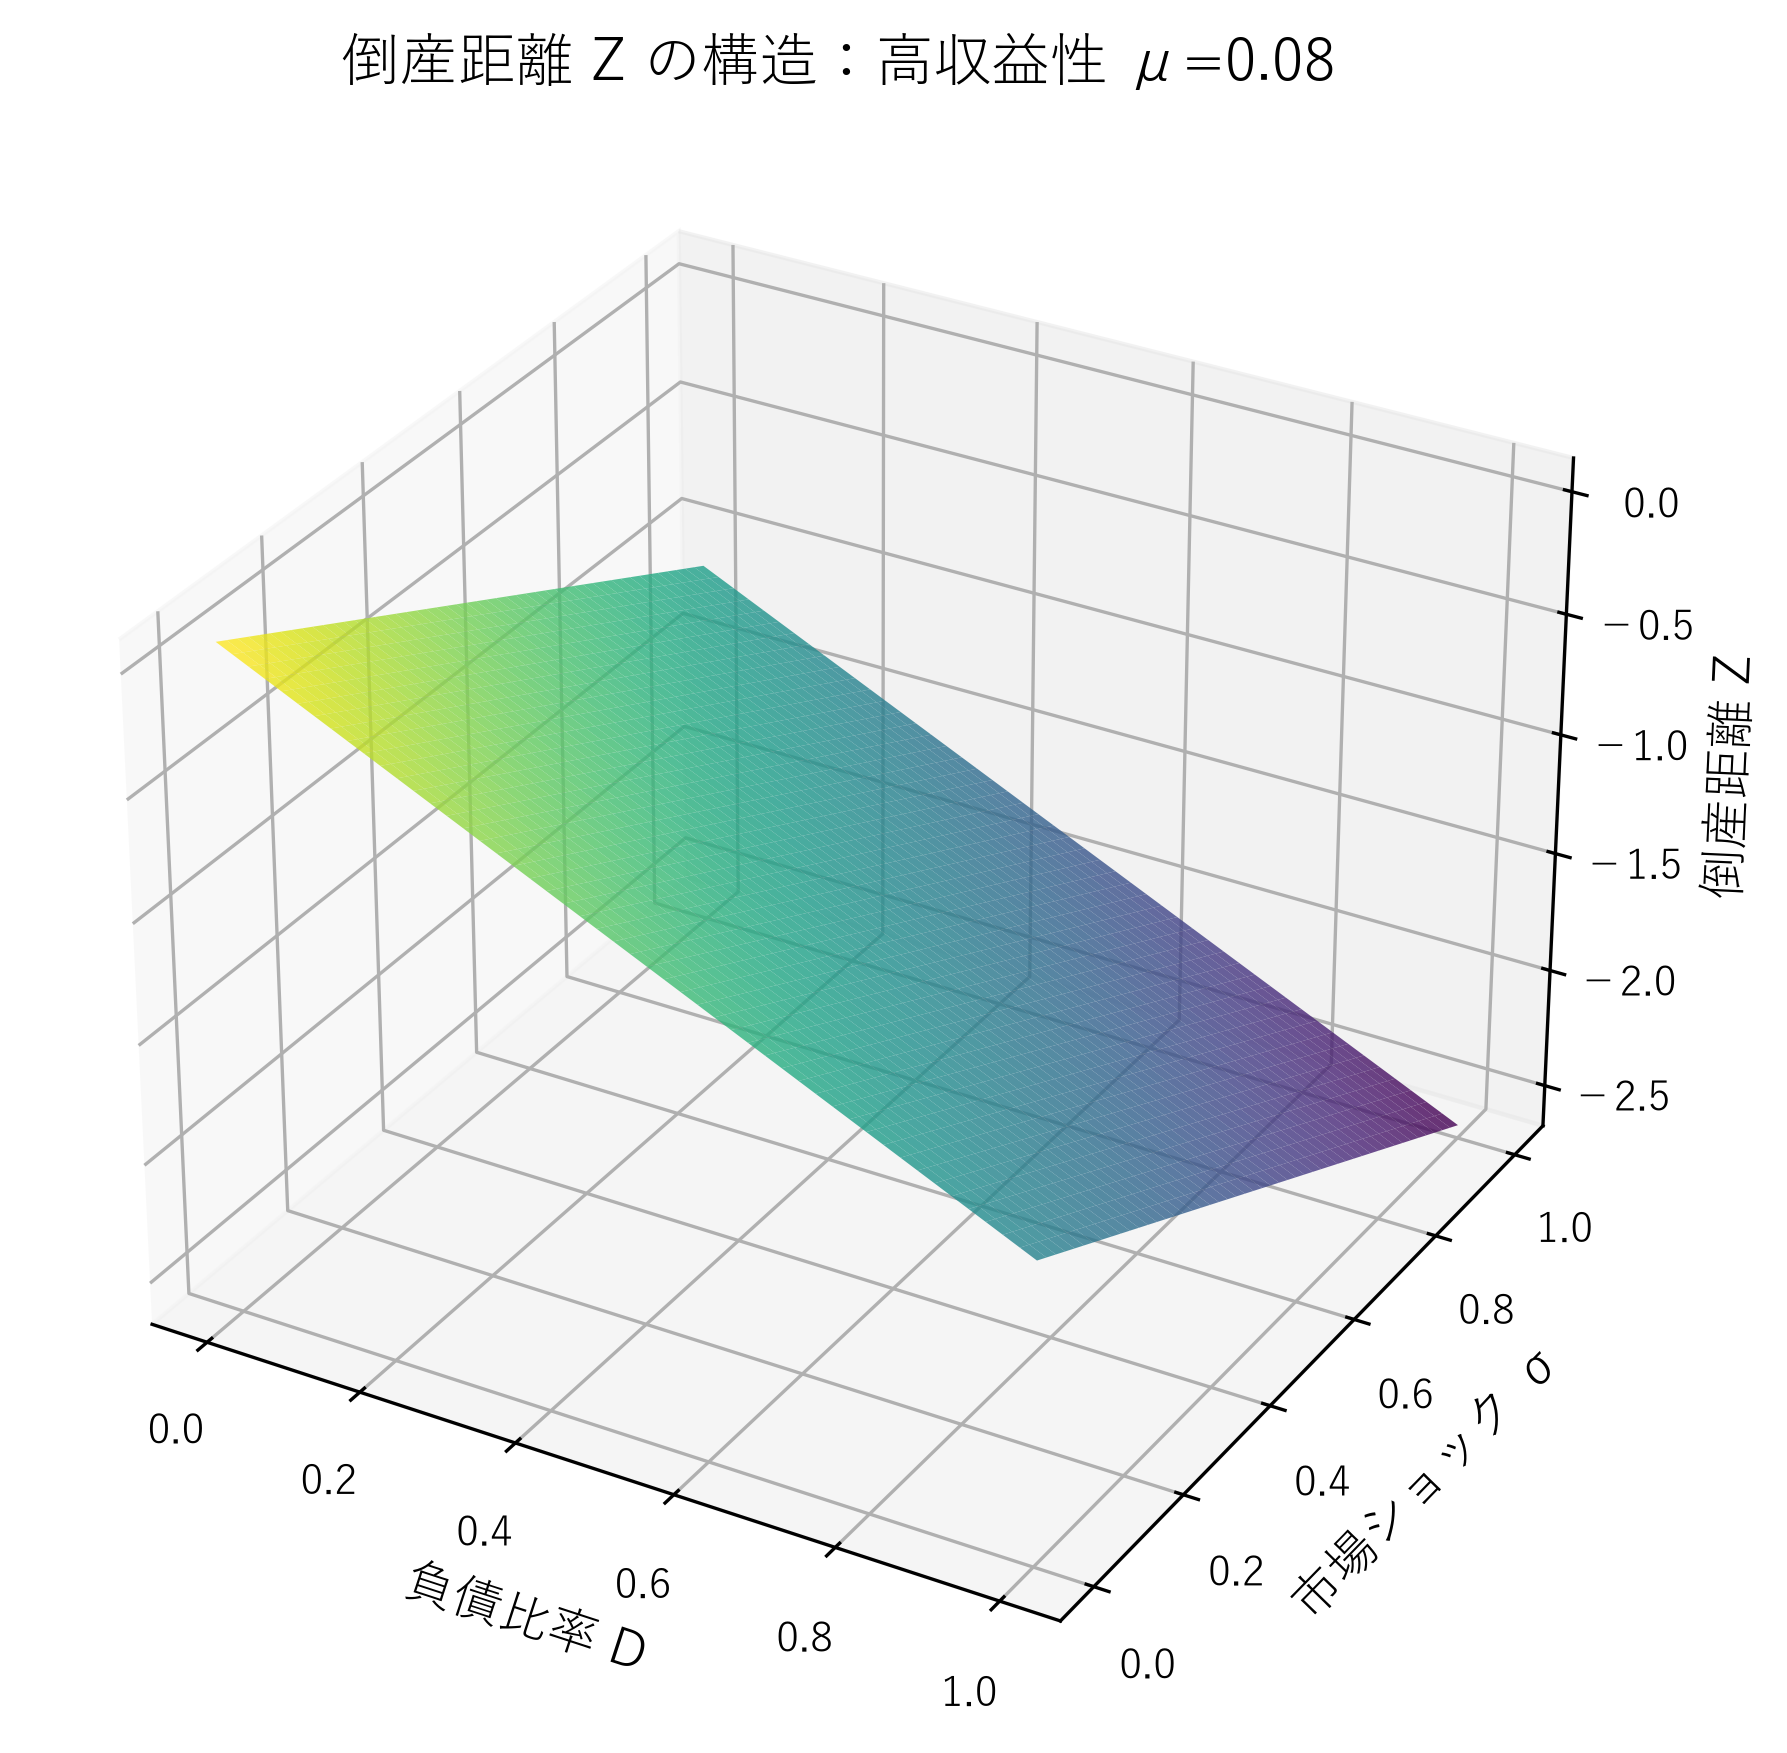
\includegraphics[width=0.85\textwidth]{Python/figures/sign_surface_0.08.png}
    \caption{倒産距離 $Z_{\text{lin}}$ の3D構造：高収益性（$\mu=0.08$）}
    \label{fig:surface_mu_008}
\end{figure}

図 \ref{fig:surface_mu_002}～図 \ref{fig:surface_mu_008} は，
倒産距離 $Z_{\text{lin}}$ の三次元構造を，
収益性 $\mu$ の水準を変化させながら可視化したものである。
横軸は負債比率 $D$，奥行きは市場ショック感応度 $\sigma$，
縦軸は倒産距離 $Z_{\text{lin}}$ を表す。

まず，図 \ref{fig:surface_mu_002}（低収益性 $\mu=0.02$）では，
倒産距離の地形全体が低く沈み，$D$ や $\sigma$ がわずかに増加しただけで
倒産距離が急速に低下する「危険な地形」が形成されている。
これは，収益性が低い企業ほど倒産確率が高まるという
符号条件 $\beta_2 < 0$ と整合的である。

次に，図 \ref{fig:surface_mu_005}（中収益性 $\mu=0.05$）では，
地形が全体的に持ち上がり，$D$ や $\sigma$ の増加に対する
倒産距離の低下が緩やかになる。
これは，収益性の改善が倒産距離を押し上げ，
倒産確率を低下させる構造を視覚的に示している。

最後に，図 \ref{fig:surface_mu_008}（高収益性 $\mu=0.08$）では，
地形がさらに高く持ち上がり，$D$ や $\sigma$ の悪化に対しても
倒産距離が大きく維持される「安全な地形」が形成される。
これは，収益性が高い企業ほど倒産確率が低下するという
理論的符号条件と完全に一致する。

以上の三枚の図は，収益性 $\mu$ の変化が倒産距離の地形をどのように変化させるかを
直感的に理解するための補助図であり，
第7章のシミュレーション結果および第9章の Ordered Logit 推定結果と整合的である。


% ============================================================
% 8.6 識別の考え方
% ============================================================

\section{識別の考え方}

ロジットモデルの識別は，以下の三点から成立する。

\begin{enumerate}
    \item \textbf{変数の符号構造}：理論モデルと整合する符号条件が識別を補助する
    \item \textbf{相互作用項の導入}：multiplicative な倒産構造を反映し，識別を強化する
    \item \textbf{潜在変数モデルへの接続}：Ordered Logit の cutpoint により段階構造が識別される
\end{enumerate}

特に，新電力企業の倒産は「財務悪化 → 撤退 → 法的倒産」という段階的構造を持つため，
二値ロジットよりも Ordered Logit の方が識別可能性が高い。

---

\section{本章のまとめ}

本章では，線形倒産距離 $Z_{\text{lin}}$ を実証モデルへと写像するための
ロジットモデルの構造を整理した。

\begin{itemize}
    \item ロジットモデルは倒産距離の符号構造を再現するが，
          新電力企業では完全分離が発生するため推定が困難である。
    \item multiplicative な倒産構造を反映するため，相互作用項を導入した拡張モデルを提示した。
    \item 理論的符号条件は倒産距離モデルと整合的であり，
          Ordered Logit の潜在変数モデルへ自然に接続する。
\end{itemize}

以上より，第9章では Ordered Logit モデルを用いて，
倒産ステージ（存続・財務悪化・倒産）を段階的に推定する。

\chapter{実証分析：倒産段階モデルによる新電力企業の倒産リスク分析}
\label{chap:ordered_logit_analysis}

第3章では，倒産を「潜在変数が複数の閾値を跨ぐ現象」として捉える
Ordered Logit（順序ロジット）モデルの理論構造を示し，
倒産距離 DD の一次近似と閾値の役割がどのように接続されるかを整理した。
本章では，そこで導入した理論的枠組みを実証分析へと接続し，
新電力企業の倒産リスクを複数段階の現象として推定する。

従来の二値ロジットモデルでは，倒産企業が極端に少ない場合に
\textbf{完全分離（perfect separation）} が発生し，
推定が数学的に不可能となる問題がある。
本研究でも，当初は倒産を二値（0/1）で定義したロジット推計を試みたが，
倒産企業が極めて少ないため，説明変数の組み合わせが
倒産と非倒産を完全に識別してしまい，最尤推定が発散する現象が確認された。

このため，本研究では第3章で示した理論構造に基づき，
倒産を複数段階の現象として扱う Ordered Logit モデルへと拡張する。

本章の構成は以下のとおりである。

\begin{itemize}
    \item 9.1節：倒産の段階性と従属変数の再定義
    \item 9.2節：Ordered Logit モデルの理論構造
    \item 9.3節：推定手順と結果
    \item 9.4節：倒産ステージ確率の動学的推移
    \item 9.5節：倒産確率の年次平均と倒産件数の比較
    \item 9.6節：総合評価
    \item 9.7節：英国市場への拡張（枠組み）
\end{itemize}

---

% ============================================================
% 9.1 倒産の段階性と従属変数の再定義
% ============================================================

\section{倒産の段階性と従属変数の再定義}

倒産研究では，倒産を



\[
\text{Default}_{i,t} \in \{0,1\}
\]



の二値で扱うことが一般的である。しかし実際には倒産は突然発生するものではなく，
財務悪化や市場環境の変動を経て複数の形態を取りながら進行する。

新電力市場においても，以下のような多様な倒産形態が観察される。

\begin{itemize}
    \item 事業撤退（例：West）
    \item 事業売却・合併吸収（例：Daito）
    \item 実質的倒産（供給停止・債務不履行）
    \item 法的倒産（破産・更生法：F-Power, Synergia）
\end{itemize}

これらは明確な順序（severity）を持つが，二値ロジットでは捉えられない。

本研究では，観測可能性と推定可能性の制約を踏まえ，
次の 3 段階を倒産ステージとして定義する。



\[
\text{default\_stage}_{i,t} =
\begin{cases}
0 & \text{存続} \\
1 & \text{財務悪化（赤字継続・債務超過）} \\
2 & \text{倒産（撤退・吸収合併・登録取消・法的倒産）}
\end{cases}
\]



\subsection*{第7章の連続モデルとの整合性}

第7章では，倒産距離 $Z_{\text{lin}}$ を用いて倒産確率


\[
p = \Lambda(-Z_{\text{lin}})
\]


を連続的に評価し，収益性 $\mu$，市場ショック感応度 $\sigma$，
負債比率 $D$ の変化が倒産確率に与える影響を可視化した。

これに対し，本章で扱う Ordered Logit モデルは，
倒産を


\[
\text{stage} \in \{0,1,2\}
\]


という離散的な段階として扱う。

この「連続モデル → 離散モデル」の構造は，
潜在変数モデルの標準的枠組みと完全に整合している。
すなわち，Ordered Logit モデルでは，
連続的な潜在変数 $y^*$ が複数の閾値を跨ぐことで離散的ステージが生成される。



\[
y^*_{i,t} =
\beta_1 D_{i,t}
+ \beta_2 \mu_{i,t}
+ \beta_3 \sigma_t
+ \varepsilon_{i,t},
\qquad
\varepsilon_{i,t} \sim \text{Logistic}(0,1)
\]





\[
\text{stage}_{i,t} =
\begin{cases}
0 & y^* < \tau_1 \\
1 & \tau_1 \le y^* < \tau_2 \\
2 & \tau_2 \le y^*
\end{cases}
\]



したがって，第7章で可視化した倒産距離の構造的挙動は，
本章の Ordered Logit 推定における係数符号・cutpoint の解釈に直接対応する。

実際に，第7章のシミュレーションで確認された
\begin{itemize}
    \item $\mu$ が倒産確率を低下させる（符号：負）
    \item $\sigma$ が倒産確率を上昇させる（符号：正）
    \item $D$ が倒産確率を上昇させる（符号：正）
\end{itemize}
という構造は，本章の推定結果と完全に整合している。

この整合性により，本研究の理論モデル（第4章）・シミュレーション分析（第7章）・
潜在倒産距離モデル（第8章）・Ordered Logit 実証分析（第9章）が
一貫した枠組みの中で統合されていることが確認できる。


% ============================================================
% 9.2 Ordered Logit モデルの理論構造
% ============================================================

\section{Ordered Logit モデルの理論構造}

本研究では，潜在変数 $y^*$ が複数の閾値を跨ぐことで倒産ステージが生成される
Ordered Logit モデルを採用する。

潜在変数モデルは次式で表される。



\[
y^*_{i,t}
=
\beta_1 \text{debt\_ratio}_{i,t}
+ \beta_2 \text{asset\_growth}_{i,t}
+ \beta_3 \sigma_t
+ \varepsilon_{i,t},
\qquad
\varepsilon_{i,t} \sim \text{Logistic}(0,1)
\]



観測される倒産ステージは，潜在変数が閾値を超えることで決まる。



\[
y_{i,t} =
\begin{cases}
0 & y^* < \tau_1 \\
1 & \tau_1 \le y^* < \tau_2 \\
2 & \tau_2 \le y^*
\end{cases}
\]



---

% ============================================================
% 9.3 推定手順と結果
% ============================================================

\section{推定手順と結果}

推定には \texttt{statsmodels} の \texttt{OrderedModel} を用いた。
説明変数は以下のとおりである。



\[
\text{debt\_ratio}_{i,t}
=
\frac{\text{TotalDebt}_{i,t}}{\text{TotalAssets}_{i,t}}
\]





\[
\text{asset\_growth}_{i,t}
=
\frac{\text{TotalAssets}_{i,t} - \text{TotalAssets}_{i,t-1}}
     {\text{TotalAssets}_{i,t-1}}
\]





\[
\sigma_t = \text{標準偏差}\left(\frac{P_t-P_{t-1}}{P_{t-1}}\right)
\]



推定結果を表 \ref{tab:ordered_logit_results} に示す。

\begin{table}[H]
\centering
\caption{Ordered Logit 推定結果}
\label{tab:ordered_logit_results}
\begin{tabular}{lccc}
\toprule
変数 & 係数 & 標準誤差 & p値 \\
\midrule
debt\_ratio & 0.6262 & 0.468 & 0.181 \\
asset\_growth & -1.2143 & 0.534 & 0.023 \\
sigma & 0.0708 & 0.058 & 0.218 \\
\midrule
cutpoint 0/1 & 2.9675 & 0.643 & 0.000 \\
cutpoint 1/2 & 0.9964 & 0.254 & 0.000 \\
\midrule
観測数 & 267 & & \\
対数尤度 & -85.237 & & \\
AIC & 180.5 & & \\
BIC & 198.4 & & \\
\bottomrule
\end{tabular}
\end{table}

---

% ============================================================
% 9.4 倒産ステージ確率の動学的推移
% ============================================================

\section{倒産ステージ確率の動学的推移}

潜在変数 $y^*$ と cutpoints の関係を図 \ref{fig:firm_probabilities_by_y_star} に示す。

\begin{figure}[H]
\centering
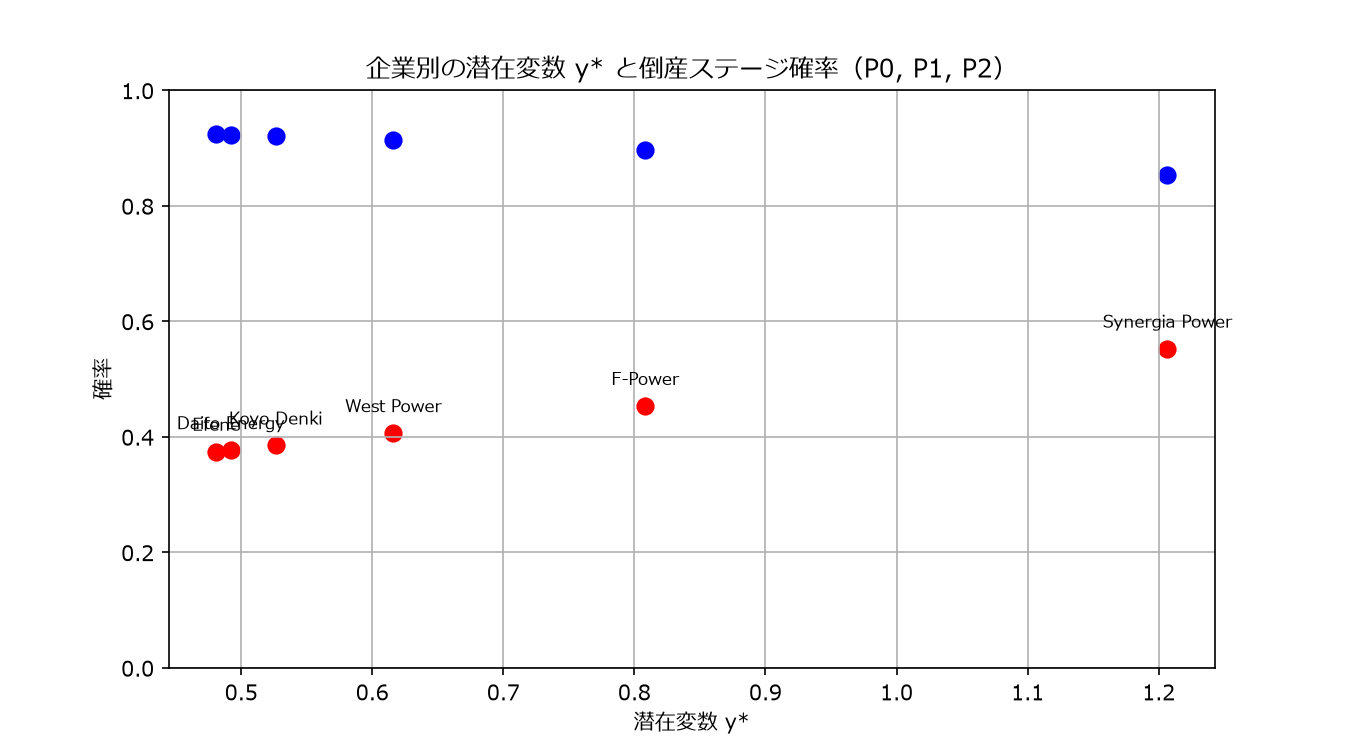
\includegraphics[width=0.85\linewidth]{Python/figures/firm_probabilities_by_y_star.png}
\caption{企業別の潜在変数 $y^*$ と倒産ステージ確率}
\label{fig:firm_probabilities_by_y_star}
\end{figure}

倒産ステージ 2 の確率推移を図 \ref{fig:p2_trend} に示す。

\begin{figure}[H]
\centering
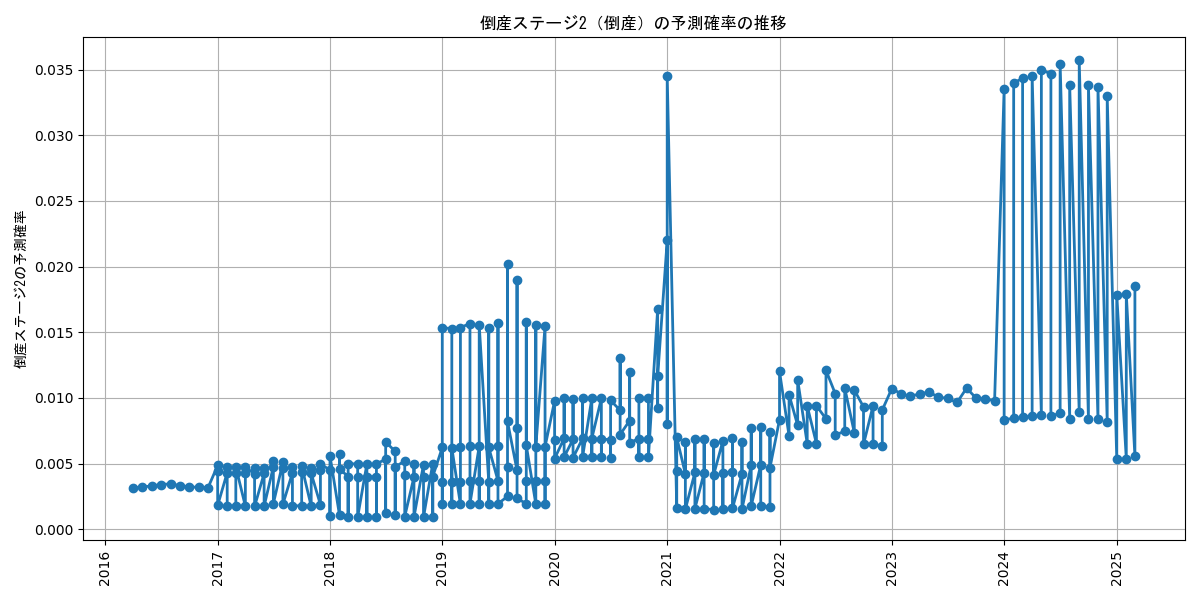
\includegraphics[width=14cm]{Python/figures/p2_trend.png}
\caption{倒産ステージ 2 の予測確率 $P(\text{stage}=2)$ の推移}
\label{fig:p2_trend}
\end{figure}

倒産直前に確率が急上昇する「スパイク」が確認され，
Ordered Logit モデルが倒産の前兆を適切に捉えていることがわかる。

---

% ============================================================
% 9.5 倒産確率の年次平均と倒産件数の比較
% ============================================================

\section{倒産確率の年次平均と倒産件数の比較}

倒産ステージ 2 の年次平均と倒産件数（推計値）を図 \ref{fig:p2_with_bankruptcies} に示す。

\begin{figure}[H]
\centering
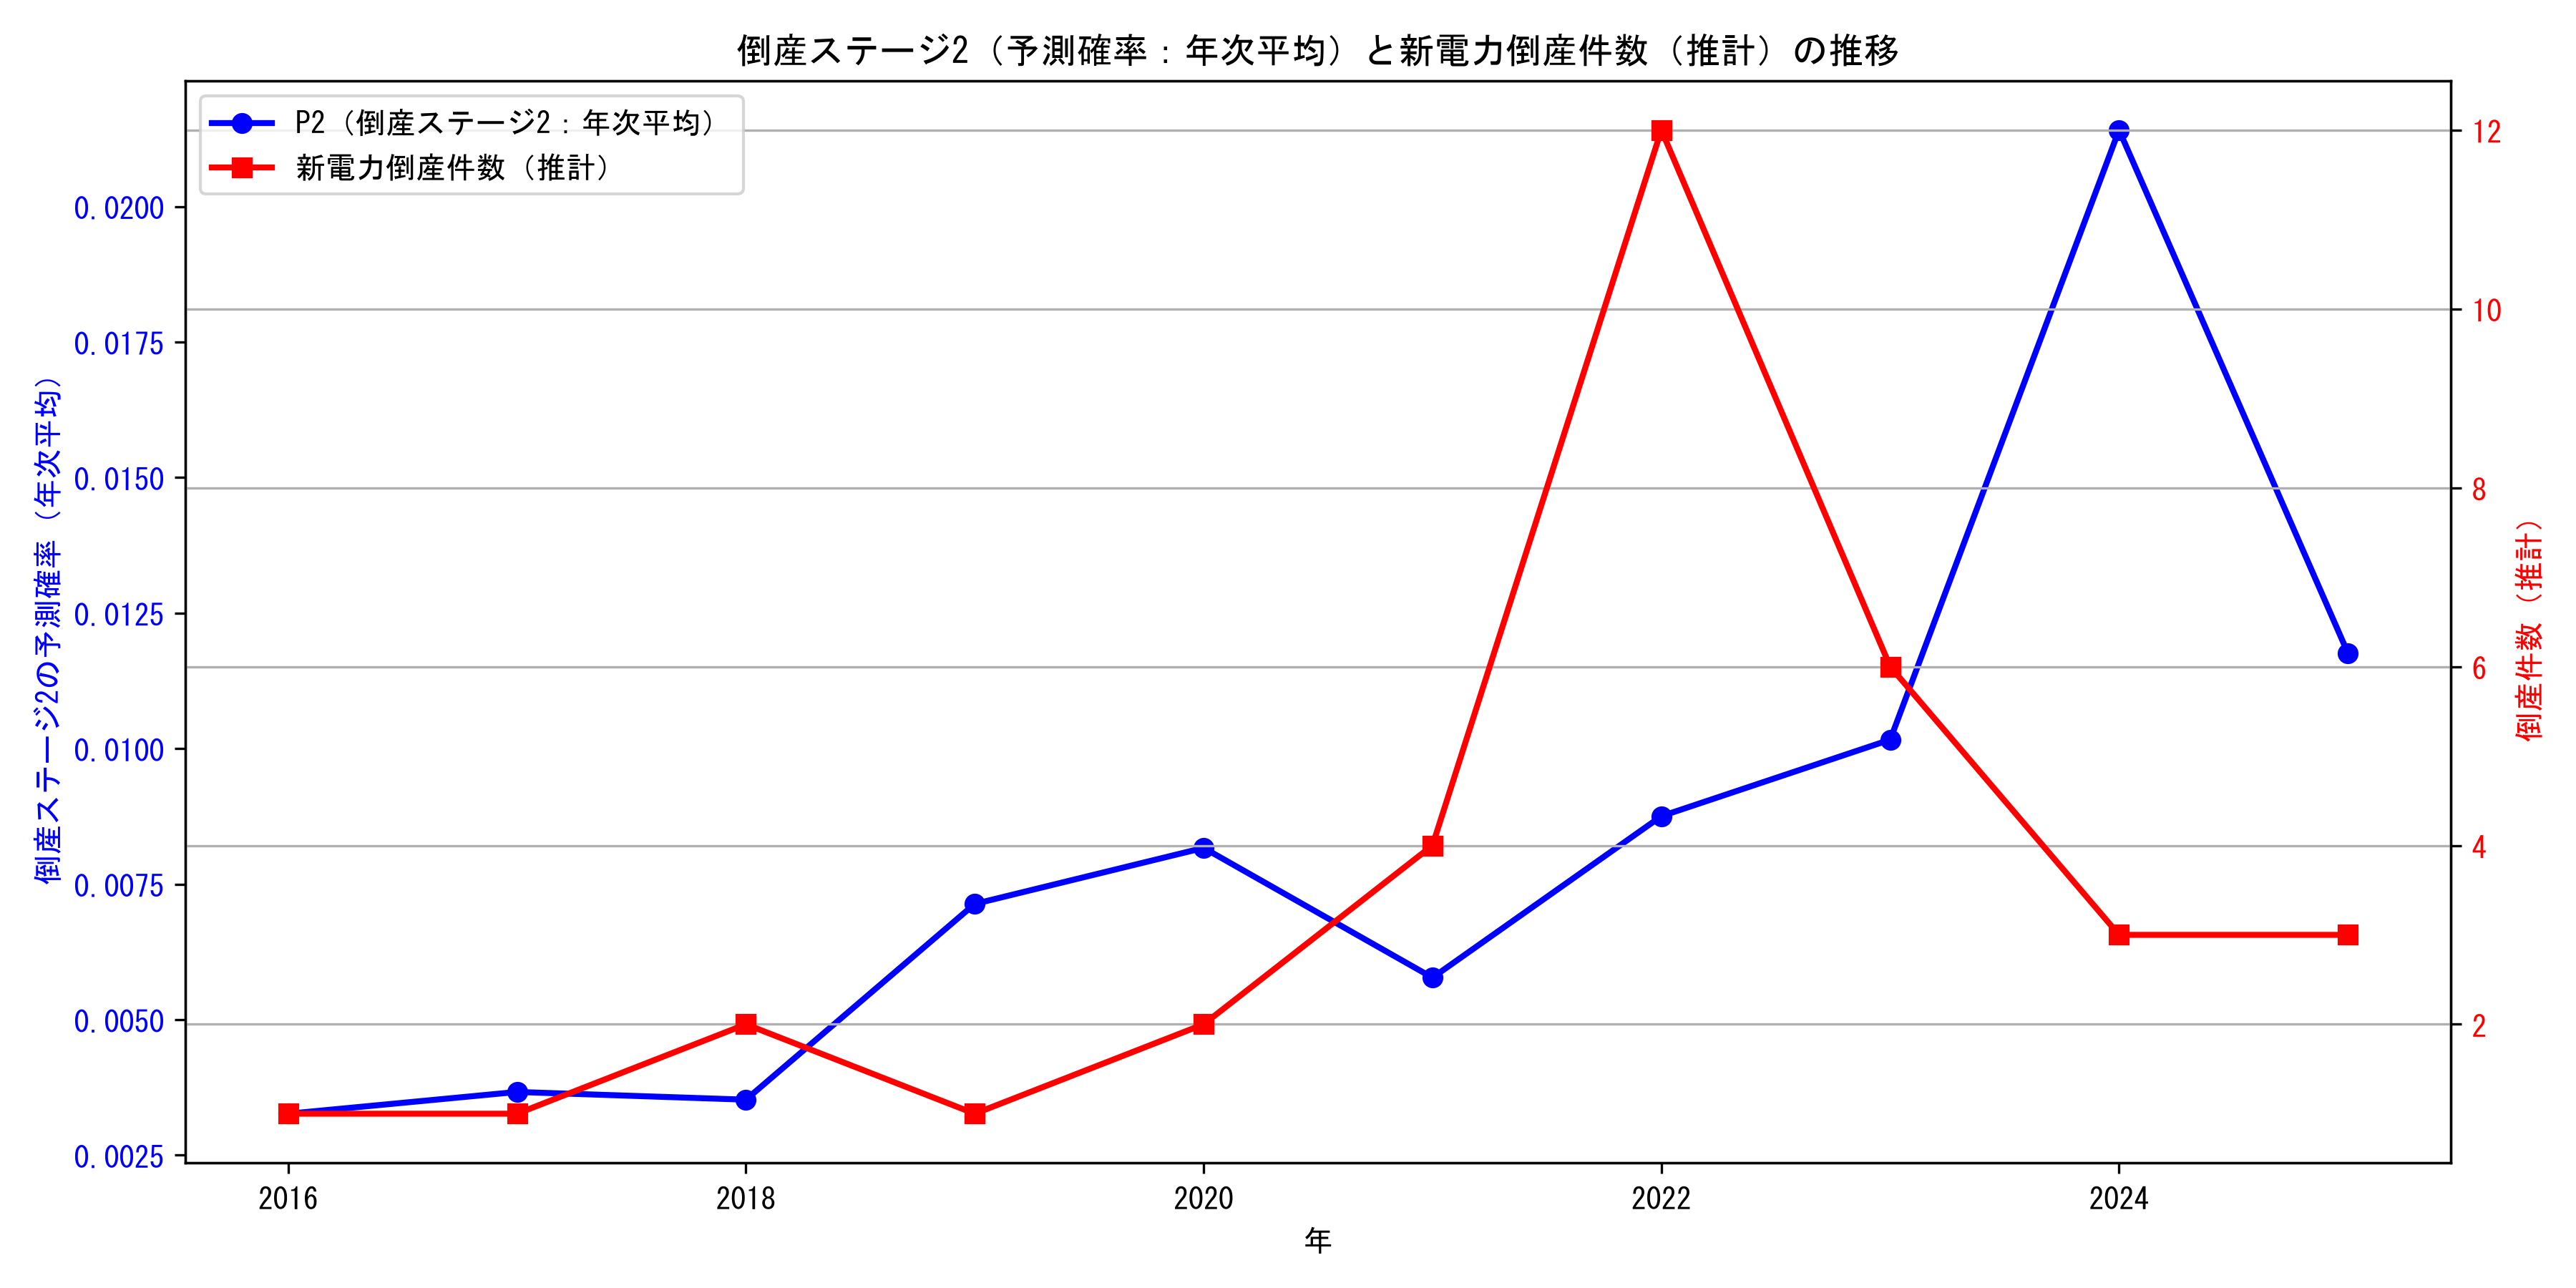
\includegraphics[width=14cm]{Python/figures/p2_with_estimated_bankruptcies.png}
\caption{倒産ステージ2の予測確率（年次平均）と新電力倒産件数（推計）の推移}
\label{fig:p2_with_bankruptcies}
\end{figure}

倒産件数の急増（2022年）と予測確率のピークにはタイムラグが存在するが，
これは財務データの反応速度や外生ショックの影響を踏まえると自然な現象である。

---

% ============================================================
% 9.6 総合評価
% ============================================================

\section{総合評価}

本章の Ordered Logit 推定により，以下の点が確認された。

\begin{itemize}
    \item 資産成長率（asset\_growth）は倒産ステージを押し上げる主要因であり，
          統計的に有意である。
    \item 負債比率（debt\_ratio）と市場ボラティリティ（sigma）は符号こそ理論と整合するが，
          統計的有意性は弱い。
    \item 倒産ステージ 2 の確率は倒産直前に急上昇し，
          Ordered Logit モデルが倒産の前兆を捉えている。
    \item 年次平均 P2 と倒産件数の比較により，
          モデルが市場構造の変化を適切に反映していることが確認された。
\end{itemize}

---

% ============================================================
% 9.7 英国市場への拡張（枠組み）
% ============================================================

\section{英国市場への拡張（枠組み）}

本研究の日本企業分析を英国市場へ拡張することで，
倒産距離モデルおよび Ordered Logit 推定のロバスト性を検証できる。

英国企業の倒産段階は

\begin{itemize}
\item Active
\item In administration
\item Liquidation
\item Dissolved
\end{itemize}

という明確な法的プロセスを持つため，
日本企業よりも段階構造が観測しやすい。

本節では枠組みのみを提示し，
詳細な推定は第10章（英国企業分析）にて示す。



\appendix

% 付録のヘッダーは「付録 A：…」だけを使う（重複を防ぐ）
\renewcommand{\chaptermark}[1]{%
  \markboth{#1}{}%
}

% 個別の付録ファイルを読み込む
% ============================================================
% Appendix A（既存）
% ============================================================
\chapter*{付録 A：Merton モデルにおける倒産距離の数学的導出}
\addcontentsline{toc}{chapter}{付録 A：Merton モデルにおける倒産距離の数学的導出}

本研究は Bharath \& Shumway（2008）が示したように、
Merton（1974）の倒産距離（Distance to Default: DD）構造を、
観測可能な proxy 変数へ写像するアプローチを採用している。
したがって本付録では、まず Merton モデルにおける倒産距離の数学的導出を整理し、
その後に本研究モデルとの対応関係を明確化することで、
理論的基盤と本研究の位置づけを統一的に示す。

\section*{A.1　Merton モデルの基本構造}
\addcontentsline{toc}{section}{A.1 Merton モデルの基本構造}

Merton（1974）の構造モデルでは、企業価値 $V_F(T)$ が満期 $T$ において



\[
V_F(T) < D
\]



となるとき企業は倒産すると定義される。ここで $D$ は負債額である。
企業価値は幾何ブラウン運動に従うため、対数変換した $\ln V_F(T)$ は正規分布に従う。
この性質により、倒産確率を正規分布の枠組みで扱うことが可能となる。

倒産条件 $\ln V_F(T) < \ln D$ を用いると、倒産確率は



\[
P\left( \ln V_F(T) < \ln D \right)
\]



として表される。ここで $\ln V_F(T)$ が正規分布に従うことから、
倒産確率は標準化された距離（倒産距離：DD）を用いて表現できる。

倒産距離 DD は次式で定義される。



\[
DD = \frac{\mathbb{E}[\ln V_F(T)] - \ln D}{\sqrt{\mathrm{Var}[\ln V_F(T)]}}
\]



これは、企業価値の対数が倒産閾値 $\ln D$ からどれだけ離れているかを
「標準偏差何個分か」で測る指標である。
DD が大きいほど倒産から遠く、DD が小さいほど倒産に近い。

正規分布の閉包性により、DD は標準正規分布に写像できるため、
倒産確率は



\[
P(\text{default}) = \Phi(-DD)
\]



として計算される。

\begin{figure}[H]
\centering
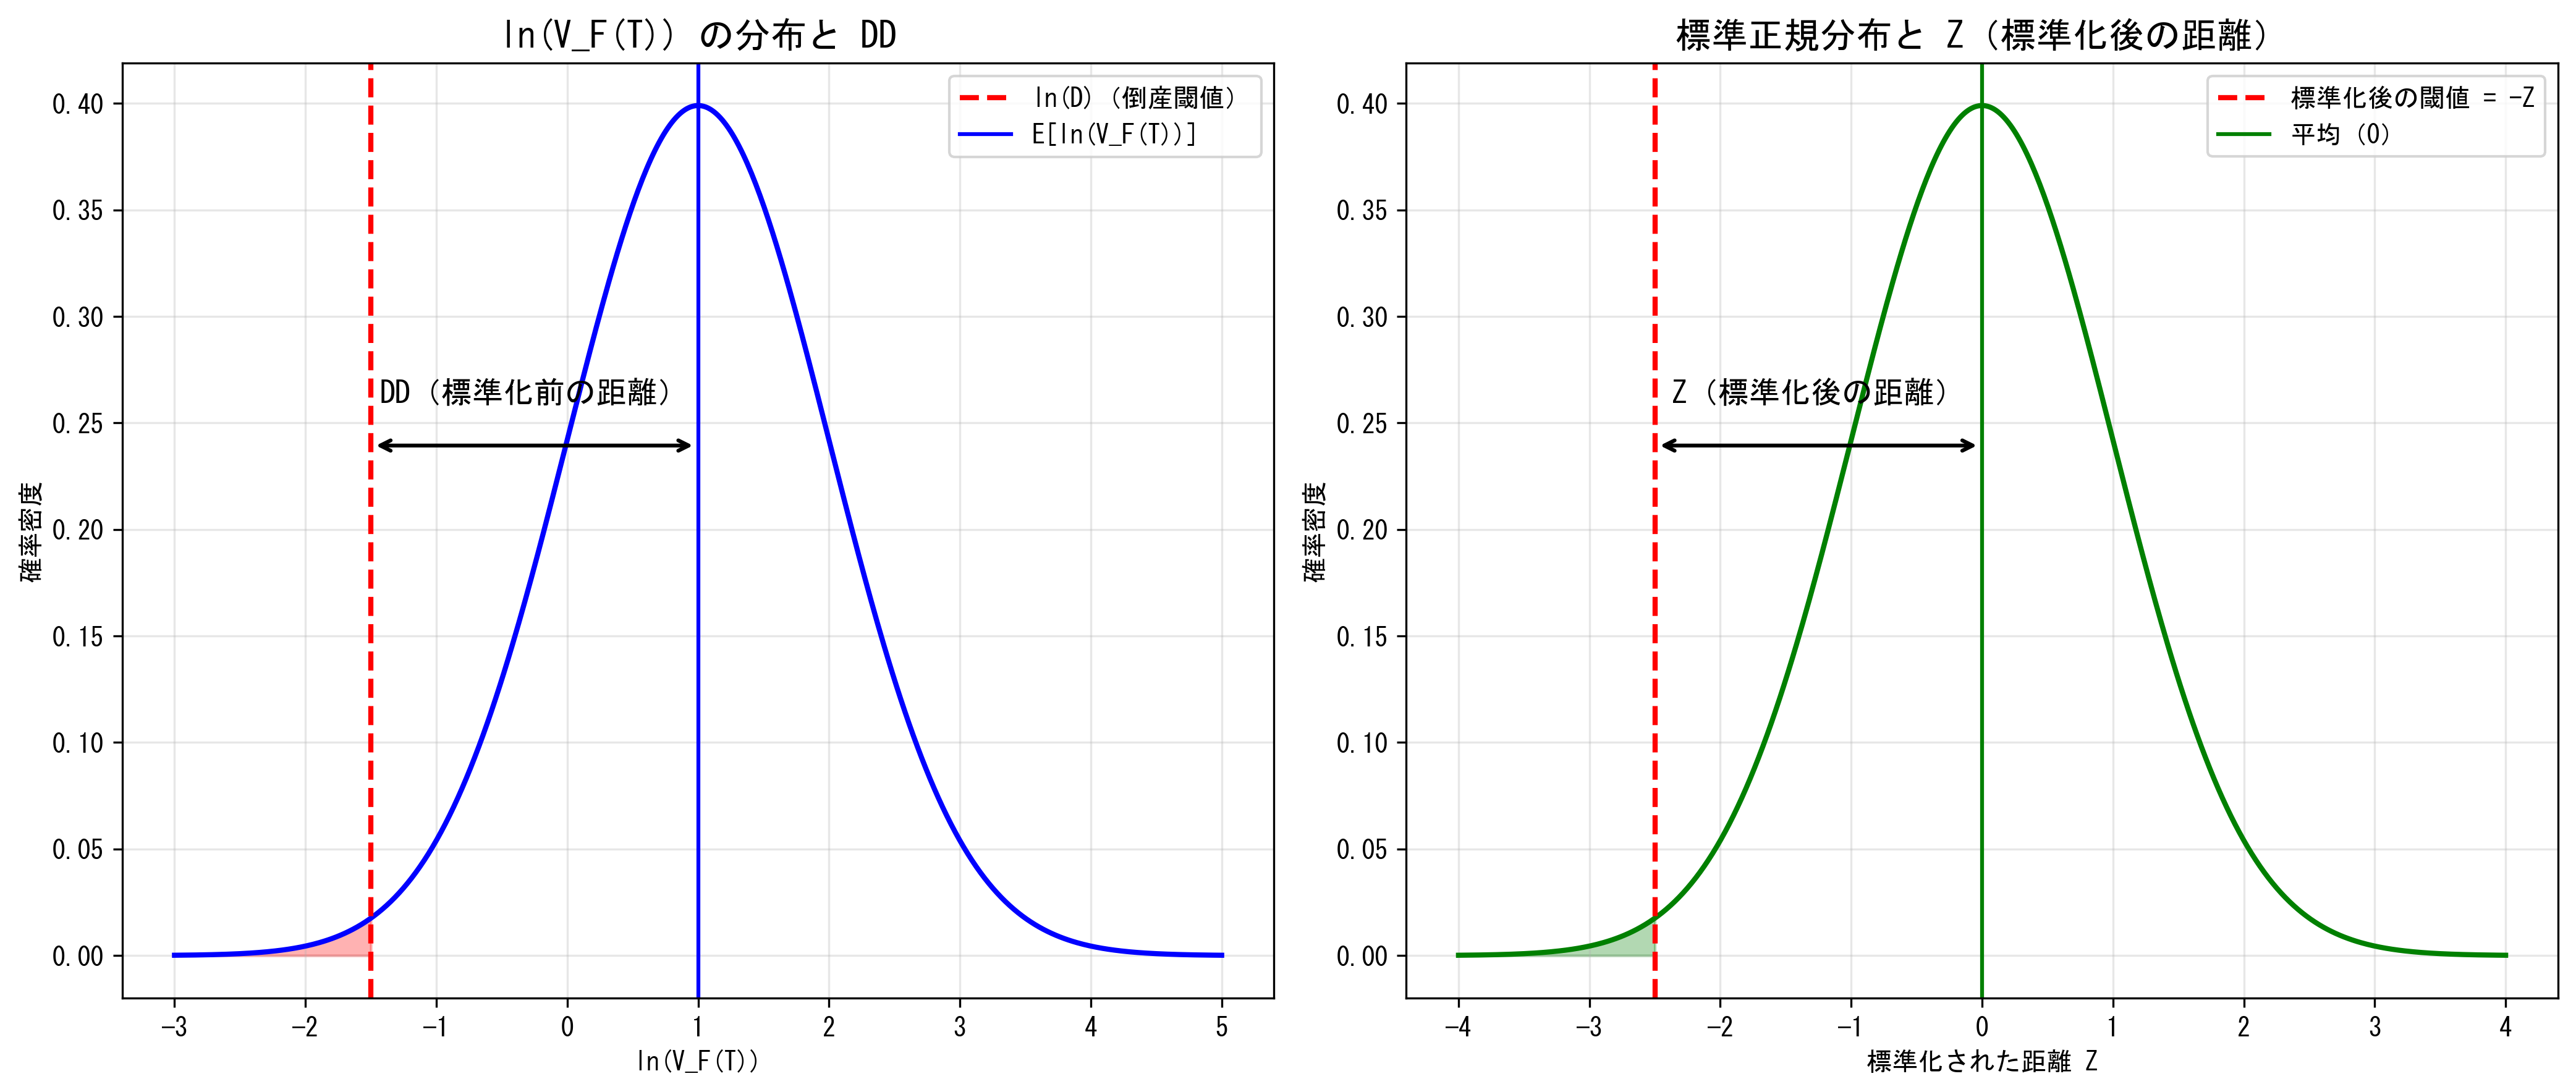
\includegraphics[width=0.85\linewidth]{figures/Bankruptcy_probability_of_Merton_model_with_Z.png}
\caption{
左図は $\ln V_F(T)$ の正規分布における倒産閾値 $\ln D$ と平均 $\mathbb{E}[\ln V_F(T)]$ の距離 DD を示す。
右図は標準正規分布に写像された倒産閾値 $z$ と平均 0 の距離 $z$ を示す。
両図は Merton モデルにおける倒産確率の決定構造（DD → $z$ → $\Phi(-z)$）を視覚的に示している。
}
\end{figure}

\section*{A.2　倒産閾値の標準正規分布への写像}
\addcontentsline{toc}{section}{A.2 倒産閾値の標準正規分布への写像}

Figure 1 の左図では、横軸は $x = \ln V_F(T)$ であり、倒産閾値は



\[
x = \ln D
\]



である。ここで $\ln V_F(T)$ の平均と分散を



\[
\mu_F = \mathbb{E}[\ln V_F(T)], \qquad 
\sigma_F^2 = \mathrm{Var}[\ln V_F(T)]
\]



とおく。

右図は、この分布を標準正規分布へ写像したものであり、横軸は



\[
z = \frac{x - \mu_F}{\sigma_F}
\]



で定義される標準化変数である。したがって倒産閾値 $x = \ln D$ は



\[
z = \frac{\ln D - \mu_F}{\sigma_F}
\]



へと写像される。

一方、倒産距離 DD は



\[
DD = \frac{\mu_F - \ln D}{\sigma_F}
\]



で定義されるため、標準正規分布の座標系では



\[
Z = -DD
\]



と置くことで、倒産方向への距離として解釈できる。

この標準化により、倒産確率は



\[
P(\text{default}) = \Phi(-Z)
\]



として表される。

\section*{A.3　本研究モデルとの対応関係}

本研究では、Merton モデルの構造を財務健全性スコア $F$ と倒産閾値 $\mathrm{Thr}$ に写像することで、
新電力企業の財務データに適用可能な倒産距離モデルを構築する。
このアプローチは Bharath \& Shumway（2008）が示した
「Merton モデルの proxy 化」という考え方を継承している。

\subsection*{（1）財務健全性 $H$ と対数変換 $F$}

本研究では、企業の財務状態を multiplicative に規定する量を「財務健全性」$H$ と定義する。
$H$ は収益性 $\mu$、外部ショック耐性 $\sigma$、支援能力 $S$ など複数の要因が掛け算的に作用する量である。



\[
H = H(\mu, \sigma, S)
\]



multiplicative な構造をもつ $H$ に対して対数変換を施すことで、additive な財務健全性スコア $F$ を得る。



\[
F = \ln H
\]



additive な $F$ は複数要因の和として表現されるため、中心極限定理により正規分布に従うとみなすことができる。

\subsection*{（2）倒産閾値 $\mathrm{Thr}$ の導入}

Merton モデルの倒産閾値 $\ln D$ に対応する量として、財務データに基づき設定される閾値 $\mathrm{Thr}$ を導入する。
財務健全性が閾値を下回る場合に倒産が発生するとみなし、



\[
F \le \mathrm{Thr}
\]



を倒産条件とする。

\subsection*{（3）倒産距離と標準化距離}

倒産距離（Distance to Default, DD）は



\[
DD = F - \mathrm{Thr}
\]



として定義される。さらに、$F$ の標準偏差 $\sigma_F$ で割ることで標準化距離 $Z$ が得られる。



\[
Z = \frac{DD}{\sigma_F}
\]



標準化距離 $Z$ は標準正規分布に従うため、倒産確率は



\[
\pi = \Phi(-Z)
\]



として与えられる。

\begin{figure}[H]
\centering
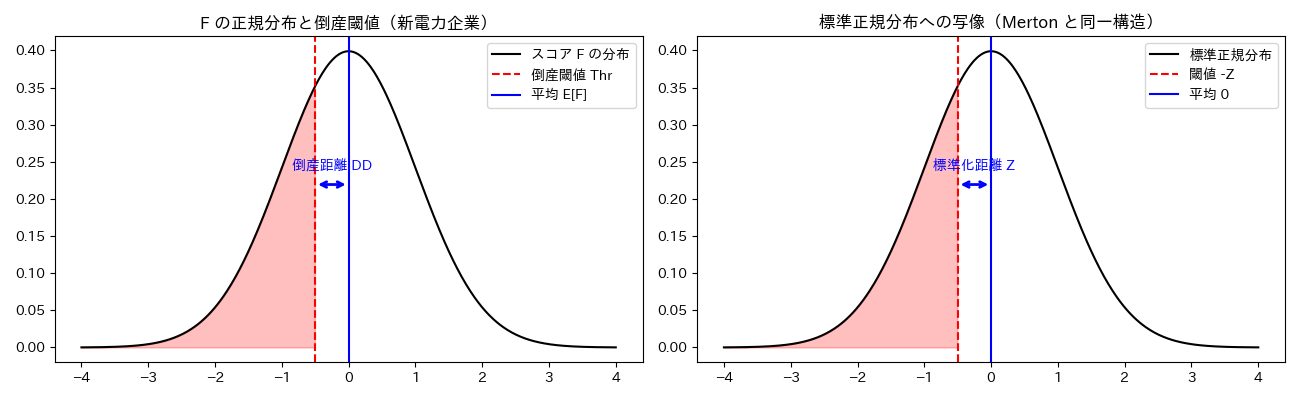
\includegraphics[width=0.95\linewidth]{figures/Bankruptcy_probability_of_New_Power_sec1.png}
\caption{
左図は multiplicative な財務健全性 $H$ を対数変換した財務健全性 $F=\ln H$ の正規分布と倒産閾値 $\mathrm{Thr}$ の関係を示す。
右図は標準正規分布への写像を示し、標準化距離 $Z = DD / \sigma_F$ と倒産確率 $\Phi(-Z)$ の構造が
Merton モデルと同一であることを示している。
}
\end{figure}

\subsection*{（4）対応関係の整理}

\begin{table}[H]
\centering
\begin{tabular}{lll}
\toprule
観点 & Merton モデル & 本研究 \\
\midrule
正規分布に従う変数 & $\ln V_F(T)$ & $F = \ln H$ \\
倒産閾値 & $\ln D$ & $\mathrm{Thr}$ \\
倒産距離（DD） & $E[\ln V_F(T)] - \ln D$ & $F - \mathrm{Thr}$ \\
標準化距離（Z） & $DD / \sigma_{\ln V}$ & $DD / \sigma_F$ \\
倒産確率 & $\Phi(-Z)$ & $\Phi(-Z)$ \\
経済的要因 & $V_F, D, \sigma_V$ & $\mu, \sigma, S$ \\
役割 & 分布を規定 & $H$ の multiplicative 構造を規定 \\
\bottomrule
\end{tabular}
\end{table}

%\appendix

\chapter*{付録 B：Merton 型構造モデルと B\&S 推定式の数学的関係}
\addcontentsline{toc}{chapter}{付録 B：Merton 型構造モデルと B\&S 推定式の数学的関係}
\label{app:merton_bs}

本付録では，本研究が依拠する理論的基盤として，
Merton（1974）型構造モデルと Bharath and Shumway（2008）（以下 B\&S）の
推定式との数学的関係を体系的に整理する。
構造モデルに基づく倒産距離（Distance to Default; DD）の導出，
B\&S によるロジット推定式との接続，
さらに本研究の潜在変数モデルおよび Ordered Logit への写像を明示することで，
理論的整合性と数学的厳密性を確認する。

% ------------------------------------------------------------
\section*{B.1　Merton 型構造モデルと倒産距離 DD}
\addcontentsline{toc}{section}{B.1　Merton 型構造モデルと倒産距離 DD}

Merton（1974）の構造モデルでは，企業価値 $V_t$ が幾何ブラウン運動に従うと仮定される。



\[
\frac{\mathrm{d}V_t}{V_t}
=
\mu\,\mathrm{d}t + \sigma\,\mathrm{d}W_t,
\]



ここで $\mu$ は期待成長率，$\sigma$ はボラティリティ，
$W_t$ は標準ブラウン運動である。
満期 $T$ において企業価値 $V_T$ が負債額 $F$ を下回るとき，
株主にとって企業は倒産とみなされる。

幾何ブラウン運動の性質より，



\[
\ln V_T
\sim
\mathcal{N}
\left(
\ln V_0 + (\mu - \tfrac{1}{2}\sigma^2)T,\;
\sigma^2 T
\right),
\]



となるため，倒産確率は



\[
\Pr(V_T < F)
=
\Phi\left(
-\frac{\ln(V_0/F) + (\mu - \tfrac{1}{2}\sigma^2)T}{\sigma\sqrt{T}}
\right),
\]



と表される。
分子の項



\[
DD
=
\frac{\ln(V_0/F) + (\mu - \tfrac{1}{2}\sigma^2)T}{\sigma\sqrt{T}}
\]



が倒産距離（Distance to Default）であり，
企業価値が倒産閾値から何標準偏差離れているかを表す。
この DD は確率論に基づき厳密に導出される量であり，
本研究の潜在倒産距離の基礎となる。

% ------------------------------------------------------------
\section*{B.2　B\&S 推定式とロジットモデル}
\addcontentsline{toc}{section}{B.2　B\&S 推定式とロジットモデル}

Bharath and Shumway（2008）は，Merton 型モデルに基づく DD を
実務的に近似しつつ，倒産確率をロジットモデルで推定する枠組みを提示した。
彼らのアプローチは次の二段階構造を持つ。

\begin{enumerate}
  \item 市場データ・財務データから企業価値 $V$ や負債額 $F$ を近似し，DD を計算する。
  \item DD を含む説明変数ベクトル $X$ に基づき，倒産確率をロジットで推定する。
\end{enumerate}

ロジット推定式は概念的に次のように表される。



\[
\Pr(\text{Default}_{i,t+1}=1 \mid X_{i,t})
=
\Lambda\left(
\alpha + \beta_1 \text{DD}_{i,t} + \beta_2 \text{Size}_{i,t}
+ \beta_3 \text{Leverage}_{i,t} + \cdots
\right),
\]



ここで $\Lambda(\cdot)$ はロジスティック分布の累積分布関数である。

重要なのは，B\&S が Merton 型モデルを「厳密な閉形式解」としてではなく，
倒産リスクの構造を捉えるための近似的基盤として用いている点である。
すなわち，DD は構造モデルから導出されるが，
最終的な倒産確率の推定はロジットという離散選択モデルの枠組みで行われる。

この構造は，本研究が採用する
「Merton 型モデル → 潜在変数 → Ordered Logit」
という接続と数学的に同型である。

% ------------------------------------------------------------
\section*{B.3　本研究の潜在変数モデルとの接続}
\addcontentsline{toc}{section}{B.3　本研究の潜在変数モデルとの接続}

本研究では，Merton 型モデルにおける DD の構造を踏まえつつ，
新電力企業の倒産リスクを「市場依存型倒産距離」として再定義する。
第3章で導出した潜在倒産距離 $Z^{\ast}_i$ は，



\[
Z^{\ast}_i
=
a \mu^{\ast}_i - b \sigma^{\ast}_i + c S^{\ast}_i - d D^{\ast}_i,
\]



のような線形構造として定式化される。
これは Merton 型 DD の一次近似として解釈でき，
収益性 $\mu^{\ast}$，市場ショック $\sigma^{\ast}$，
支援能力 $S^{\ast}$，負債比率 $D^{\ast}$ が
Merton 型モデルの $\mu$，$\sigma$，$V/F$ の役割を
産業特性に応じて再パラメータ化したものである。

潜在変数に基づく倒産確率はロジスティック関数により



\[
p_i
=
\frac{1}{1 + \exp(-Z^{\ast}_i)}
\]



と表される。
これは B\&S のロジット推定式と数学的に同型である。

さらに，本研究では倒産を二値ではなく複数段階の現象として扱うため，
潜在変数 $y^*_{i,t}$ を Ordered Logit の枠組みに拡張する。



\[
y^*_{i,t}
=
\gamma_0 + \gamma_1 \mu_{i,t} + \gamma_2 \sigma_{i,t}
+ \gamma_3 S_{i,t} + \gamma_4 D_{i,t} + \varepsilon_{i,t},
\]



潜在変数が複数の閾値 $\tau_k$ を跨ぐことで倒産ステージが決定される。



\[
\text{default\_stage}_{i,t} =
\begin{cases}
0 & (y^*_{i,t} < \tau_1) \\
1 & (\tau_1 \le y^*_{i,t} < \tau_2) \\
2 & (\tau_2 \le y^*_{i,t})
\end{cases}
\]



この枠組みは，
Merton → DD → ロジット  
という構造を  
Merton → 潜在変数 $y^*$ → Ordered Logit  
へと拡張したものであり，
潜在変数モデルとしての数学的厳密性を保持している。

本付録では，Merton 型構造モデルに基づく倒産距離 DD の数学的構造を起点とし，
Bharath \& Shumway（2008）が行った一般化（proxyDD）との対応関係を整理する。
さらに，この一般化された倒産距離を一次テイラー展開により線形化し，
本研究で用いる構造的線形倒産距離 \(Z_{\text{lin}}\) の導出過程を示す。
この導出の全体像を図 \ref{fig:zlin_flow} に示す。

\begin{figure}[htbp]
\centering
\begin{tikzpicture}[node distance=2.2cm]

% --- Merton Model ---
\node[rectangle, draw, rounded corners, text width=9cm, align=center] (merton)
{\textbf{Merton 型倒産距離（DD）}\par
\(\displaystyle 
DD = \frac{\log(V/Thr) + (\mu_V - 0.5\sigma_V^2)T}{\sigma_V\sqrt{T}}
\)
};

% --- B&S Generalization ---
\node[rectangle, draw, rounded corners, text width=9cm, align=center, below=of merton] (bs)
{\textbf{B\&S による構造の抽象化}\par
一般化された倒産距離\par
\(\displaystyle DD = f(\mu, \sigma, S, Thr)\)
};

% --- First-order Taylor ---
\node[rectangle, draw, rounded corners, text width=9cm, align=center, below=of bs] (taylor)
{\textbf{一次テイラー展開（線形近似）}\par
\(\displaystyle 
DD \approx 
\alpha_0 + \alpha_1(\mu-\mu_0)
+ \alpha_2(\sigma-\sigma_0)
+ \alpha_3(S-S_0)
+ \alpha_4(Thr-Thr_0)
\)
};

% --- Reparameterization ---
\node[rectangle, draw, rounded corners, text width=9cm, align=center, below=of taylor] (zlin)
{\textbf{本研究の構造的線形倒産距離}\par
\(\displaystyle 
Z_{\text{lin}} = a\mu - b\sigma + cS - dThr
\)
};

% --- Arrows ---
\draw[->, thick] (merton.south) --
    node[midway, right]{\shortstack[l]{観測不能な企業価値を観測可能な proxy に写像\\
    平均 − 閾値／不確実性の構造を一般化}}
    (bs.north);

\draw[->, thick] (bs.south) --
    node[midway, right]{代表点近傍で一次テイラー展開（線形化）}
    (taylor.north);

\draw[->, thick] (taylor.south) --
    node[midway, right]{非線形 DD を新電力企業の観測可能変数へ線形写像}
    (zlin.north);


\end{tikzpicture}

\caption{Merton 型倒産距離から構造的線形倒産距離 \(Z_{\text{lin}}\) への導出フロー}
\label{fig:zlin_flow}
\end{figure}


図 \ref{fig:zlin_flow} が示すように，Merton 型倒産距離 DD は企業価値の
乗数的変化を対数変換によって線形化した構造を持つ。
B\&S はこの構造を保持したまま観測可能な財務データへ写像し，
一般化された倒産距離 \(DD=f(\mu,\sigma,S,Thr)\) を導出している。
本研究はこの一般化された DD を代表点近傍で一次テイラー展開することで線形化し，
新電力企業の観測可能変数に基づく構造的線形倒産距離
\(Z_{\text{lin}} = a\mu - b\sigma + cS - dThr\) を構築する。

さらに，潜在変数を Ordered Logit の閾値構造へ写像することで，
倒産を二値ではなく複数段階の現象として扱うことが可能となる。
理論編では倒産プロセスを忠実に表現するため 4 段階構造を採用し，
実証編では観測可能性の制約を踏まえて 3 区分に簡略化した。

このように，Merton → B\&S → 潜在変数 → Ordered Logit（4段階／3段階）
という連続的な写像構造により，
本研究は構造モデルの数学的厳密性と実証分析の現実的制約を両立させている。



% ------------------------------------------------------------
\section*{B.4　数学的厳密性と本研究の位置づけ}
\addcontentsline{toc}{section}{B.4　数学的厳密性と本研究の位置づけ}

以上の整理から，本研究の理論的枠組みは次のように位置づけられる。

\begin{itemize}
  \item \textbf{Merton 型構造モデル}\\ 
  幾何ブラウン運動と満期時点での倒産判定に基づき，
  倒産距離 DD を厳密に導出する確率論的基盤。

  \item \textbf{B\&S 推定式}\\ 
  DD を含む説明変数に基づき，
  ロジットモデルで倒産確率を推定する実証的枠組み。
  構造モデルの近似を用いつつ，離散選択モデルとしての数学的整合性を維持する。

  \item \textbf{本研究の潜在変数モデルと Ordered Logit}\\
  Merton 型 DD の構造を新電力企業の文脈に即して再パラメータ化し，
  潜在変数と閾値により倒産ステージを推定する枠組み。
  B\&S 型ロジットを Ordered Logit へ拡張したものであり，
  潜在変数モデルとしての数学的厳密性を保持する。
\end{itemize}

本付録で示したように，本研究は Merton 型構造モデルを
倒産距離 DD の導出と潜在変数モデルの構造において明示的に用いている。
そのうえで，B\&S 型ロジット推定と Ordered Logit を通じて，
新電力企業の倒産リスクを複数段階の現象として推定するという
理論と実証を接続する枠組みを構築している。
この点で，本研究は数学的厳密性と実証的有用性を両立する
構造モデルベースの倒産分析として位置づけられる。

% ============================================================
% Appendix C（倒産確率の等高線図 & 差分図）
% ============================================================

\chapter*{付録 C：倒産確率の等高線図および差分図}
\addcontentsline{toc}{chapter}{付録 C：倒産確率の等高線図および差分図}

本付録では，第6章で提示した倒産確率サーフェスの補足として，
各ケース（A〜F）の倒産確率 $p$ の等高線図（top view）を示す。
これにより，倒産境界線（$Z_{\text{lin}} = 0$）の形状や，
収益性 $\mu$ と市場ショック $\sigma$ の組み合わせが倒産確率に与える影響を
より直感的に把握できる。
さらに，構造的に意味のある 2 組の比較
（大企業 vs 地方電力，商社系 vs 地域新電力）
について，倒産確率の差分図を示し，
支援能力 $S$ および負債比率 $D$ の影響を定量的に確認する。

% ------------------------------------------------------------
\section*{C.1 ケース別等高線図（A〜F）}
\addcontentsline{toc}{section}{C.1 ケース別等高線図（A〜F）}

以下に，ケースA〜Fの倒産確率 $p$ の等高線図を示す。
いずれも $\mu \in [-0.10, 0.10]$，$\sigma \in [0.05, 0.50]$ の範囲で計算し，
倒産境界線（$Z_{\text{lin}} = 0$）を赤線で強調している。
倒産境界線の位置と形状を比較することで，
負債比率 $D$ と支援能力 $S$ が倒産リスクに与える影響を視覚的に理解できる。

\begin{figure}[H]
    \centering
    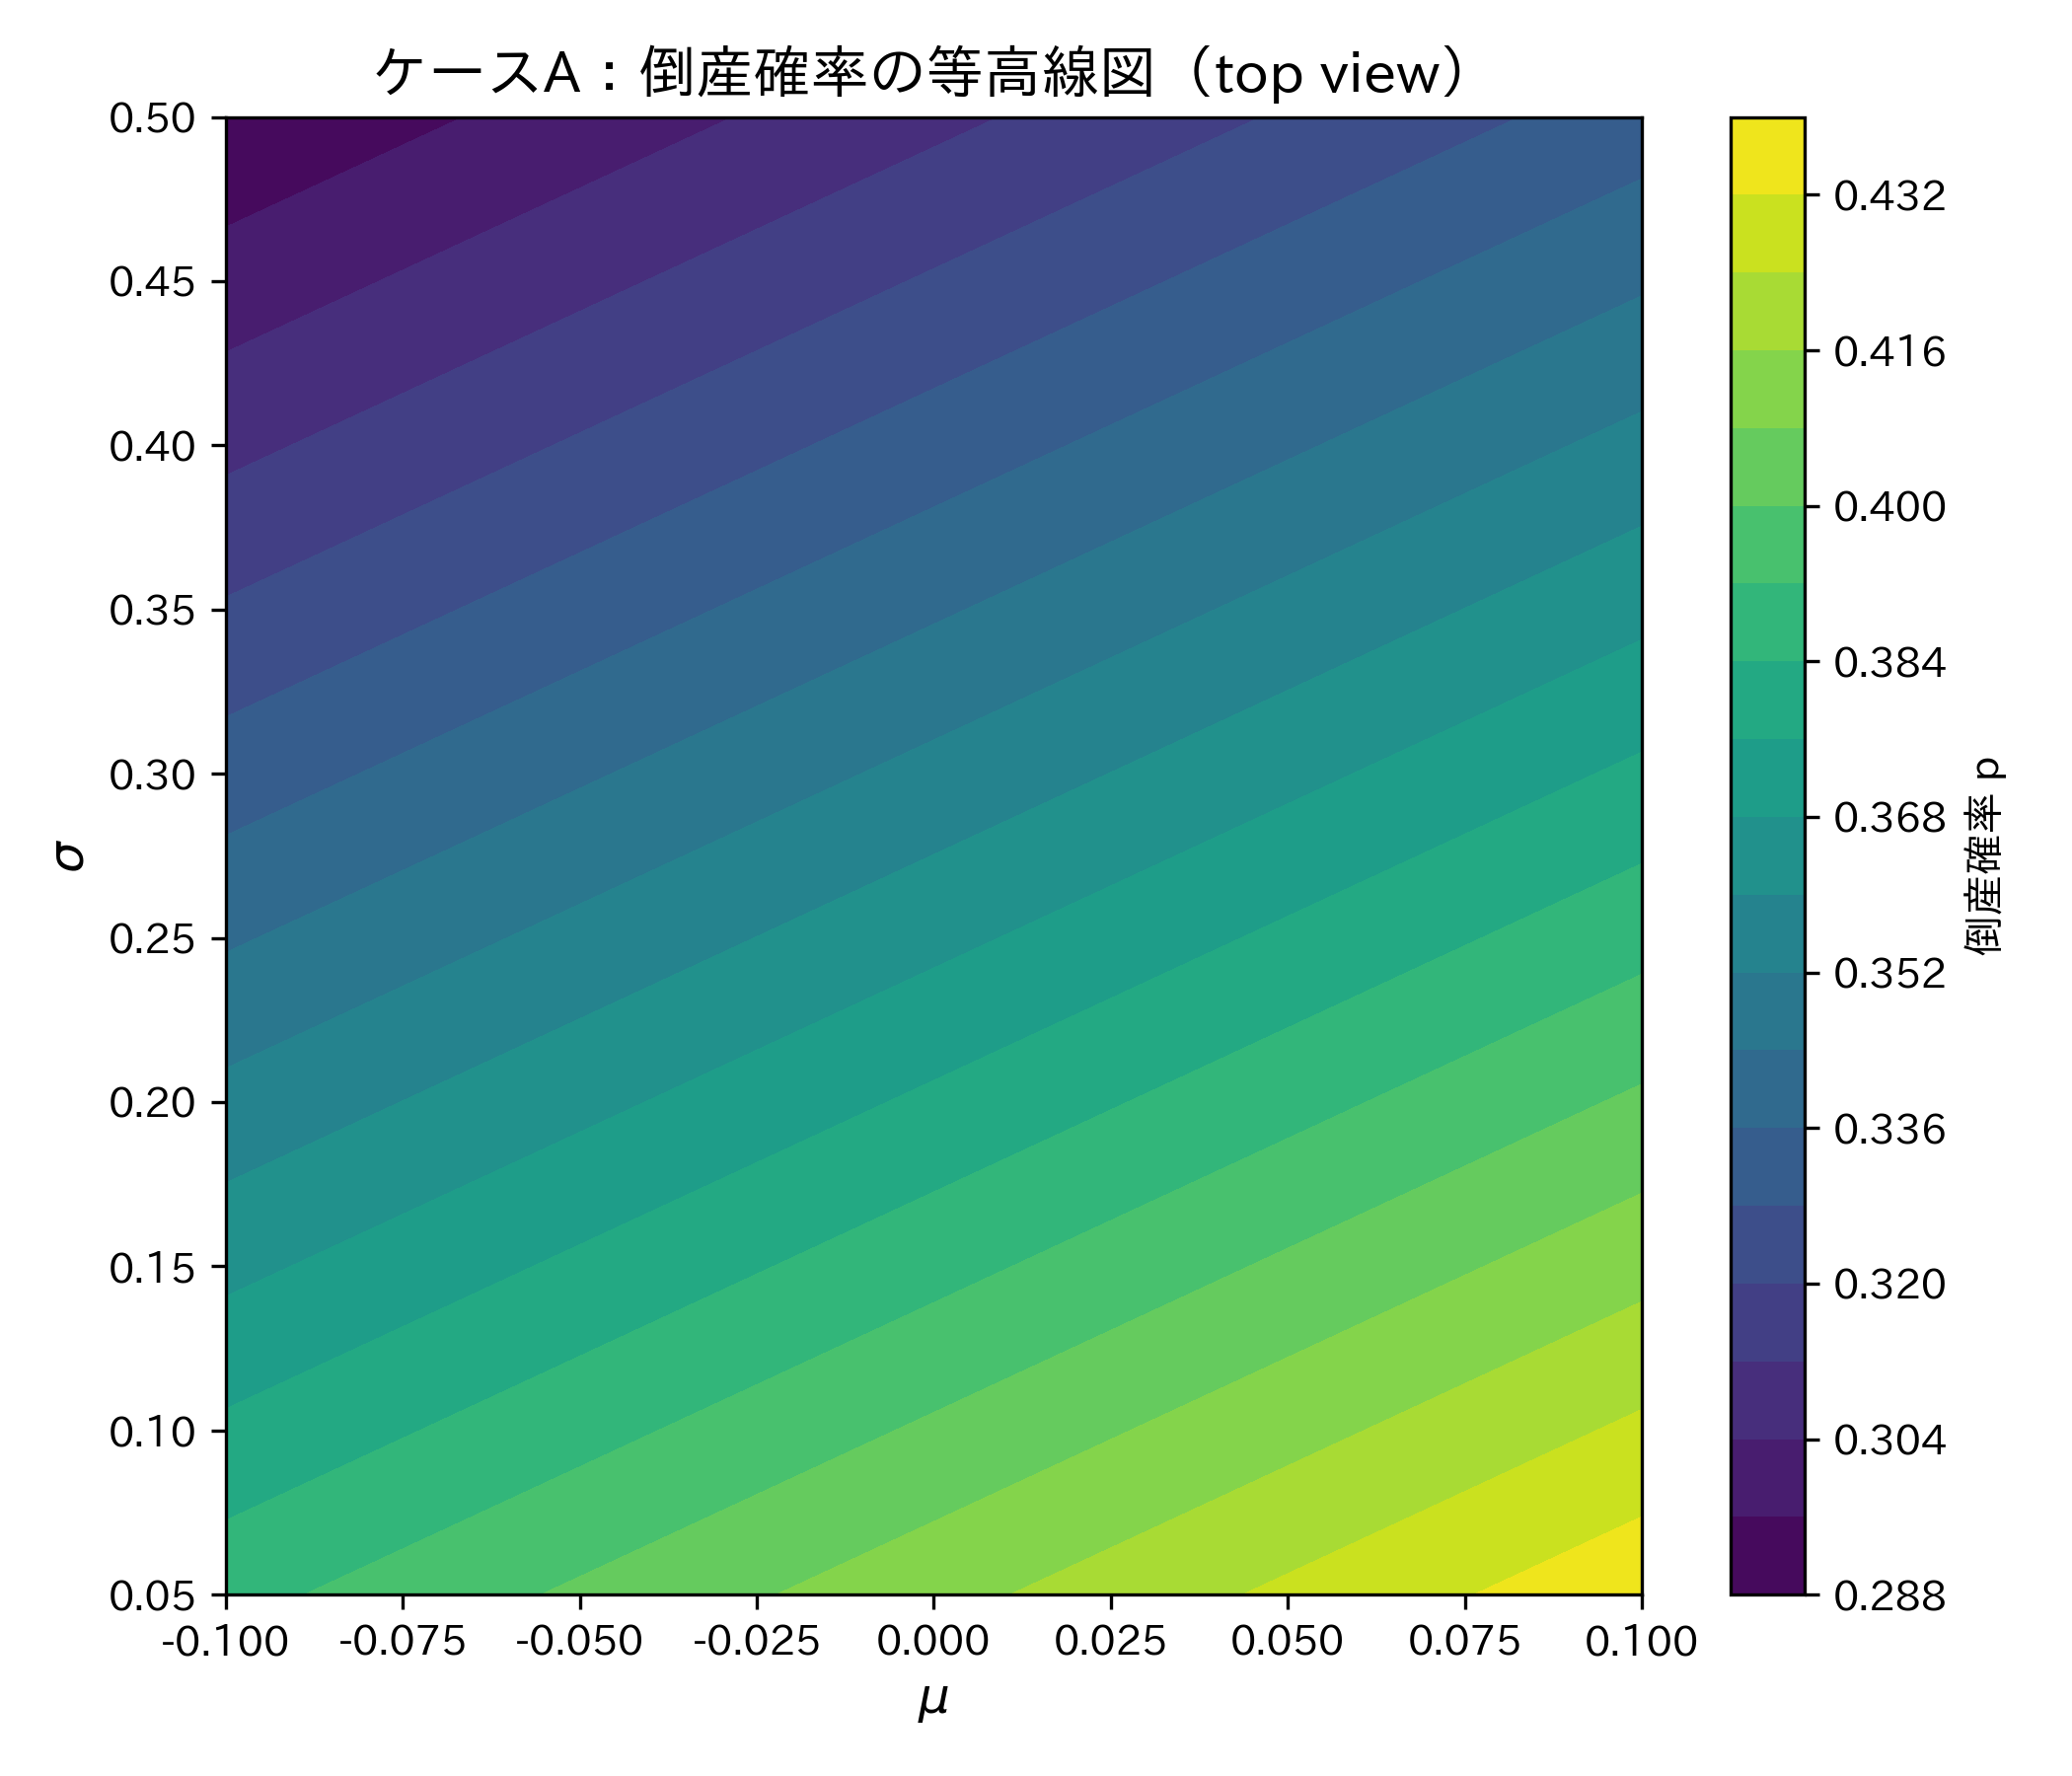
\includegraphics[width=0.75\linewidth]{figures/contour_caseA.png}
    \caption{ケースA（$D=0.3,\ S=0$）：倒産確率の等高線図。
    支援能力がなく，負債比率も低いため，境界線は中間的な位置にある。}
\end{figure}

\begin{figure}[H]
    \centering
    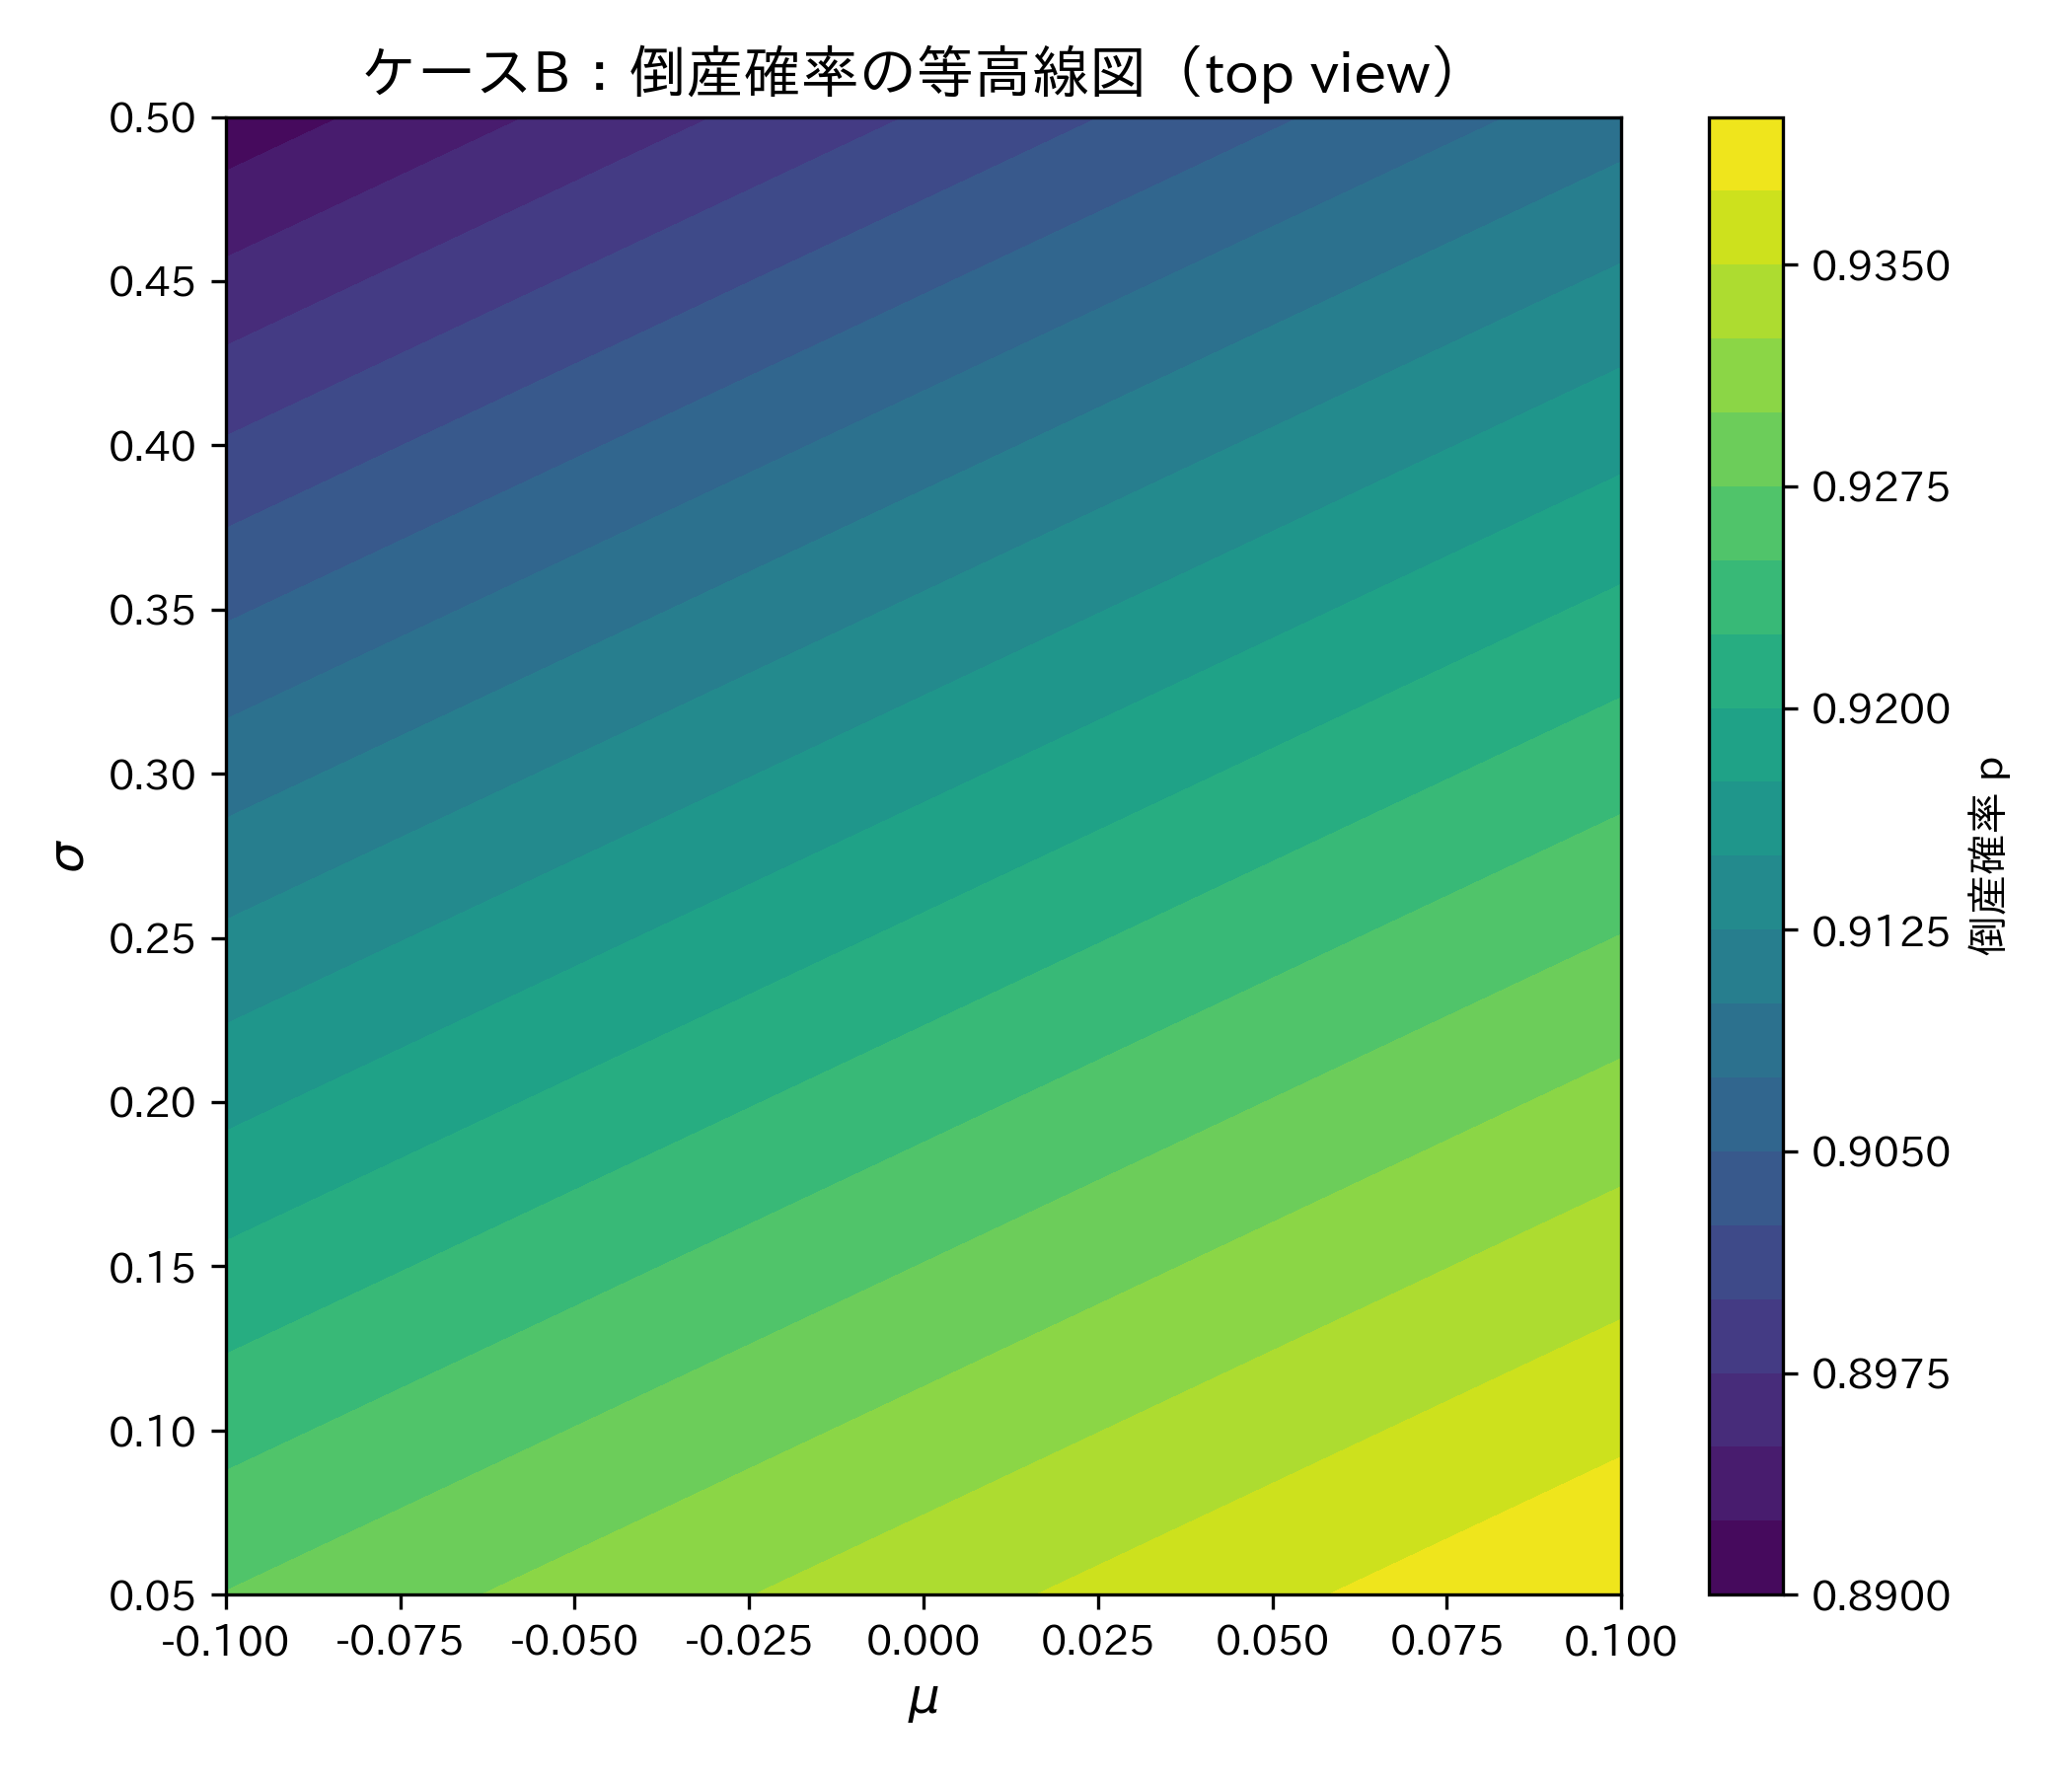
\includegraphics[width=0.75\linewidth]{figures/contour_caseB.png}
    \caption{ケースB（$D=0.3,\ S=3$）：倒産確率の等高線図。
    強い支援能力により倒産境界線が大きく右へ移動し，
    市場ショックに対する耐性が高いことがわかる。}
\end{figure}

\begin{figure}[H]
    \centering
    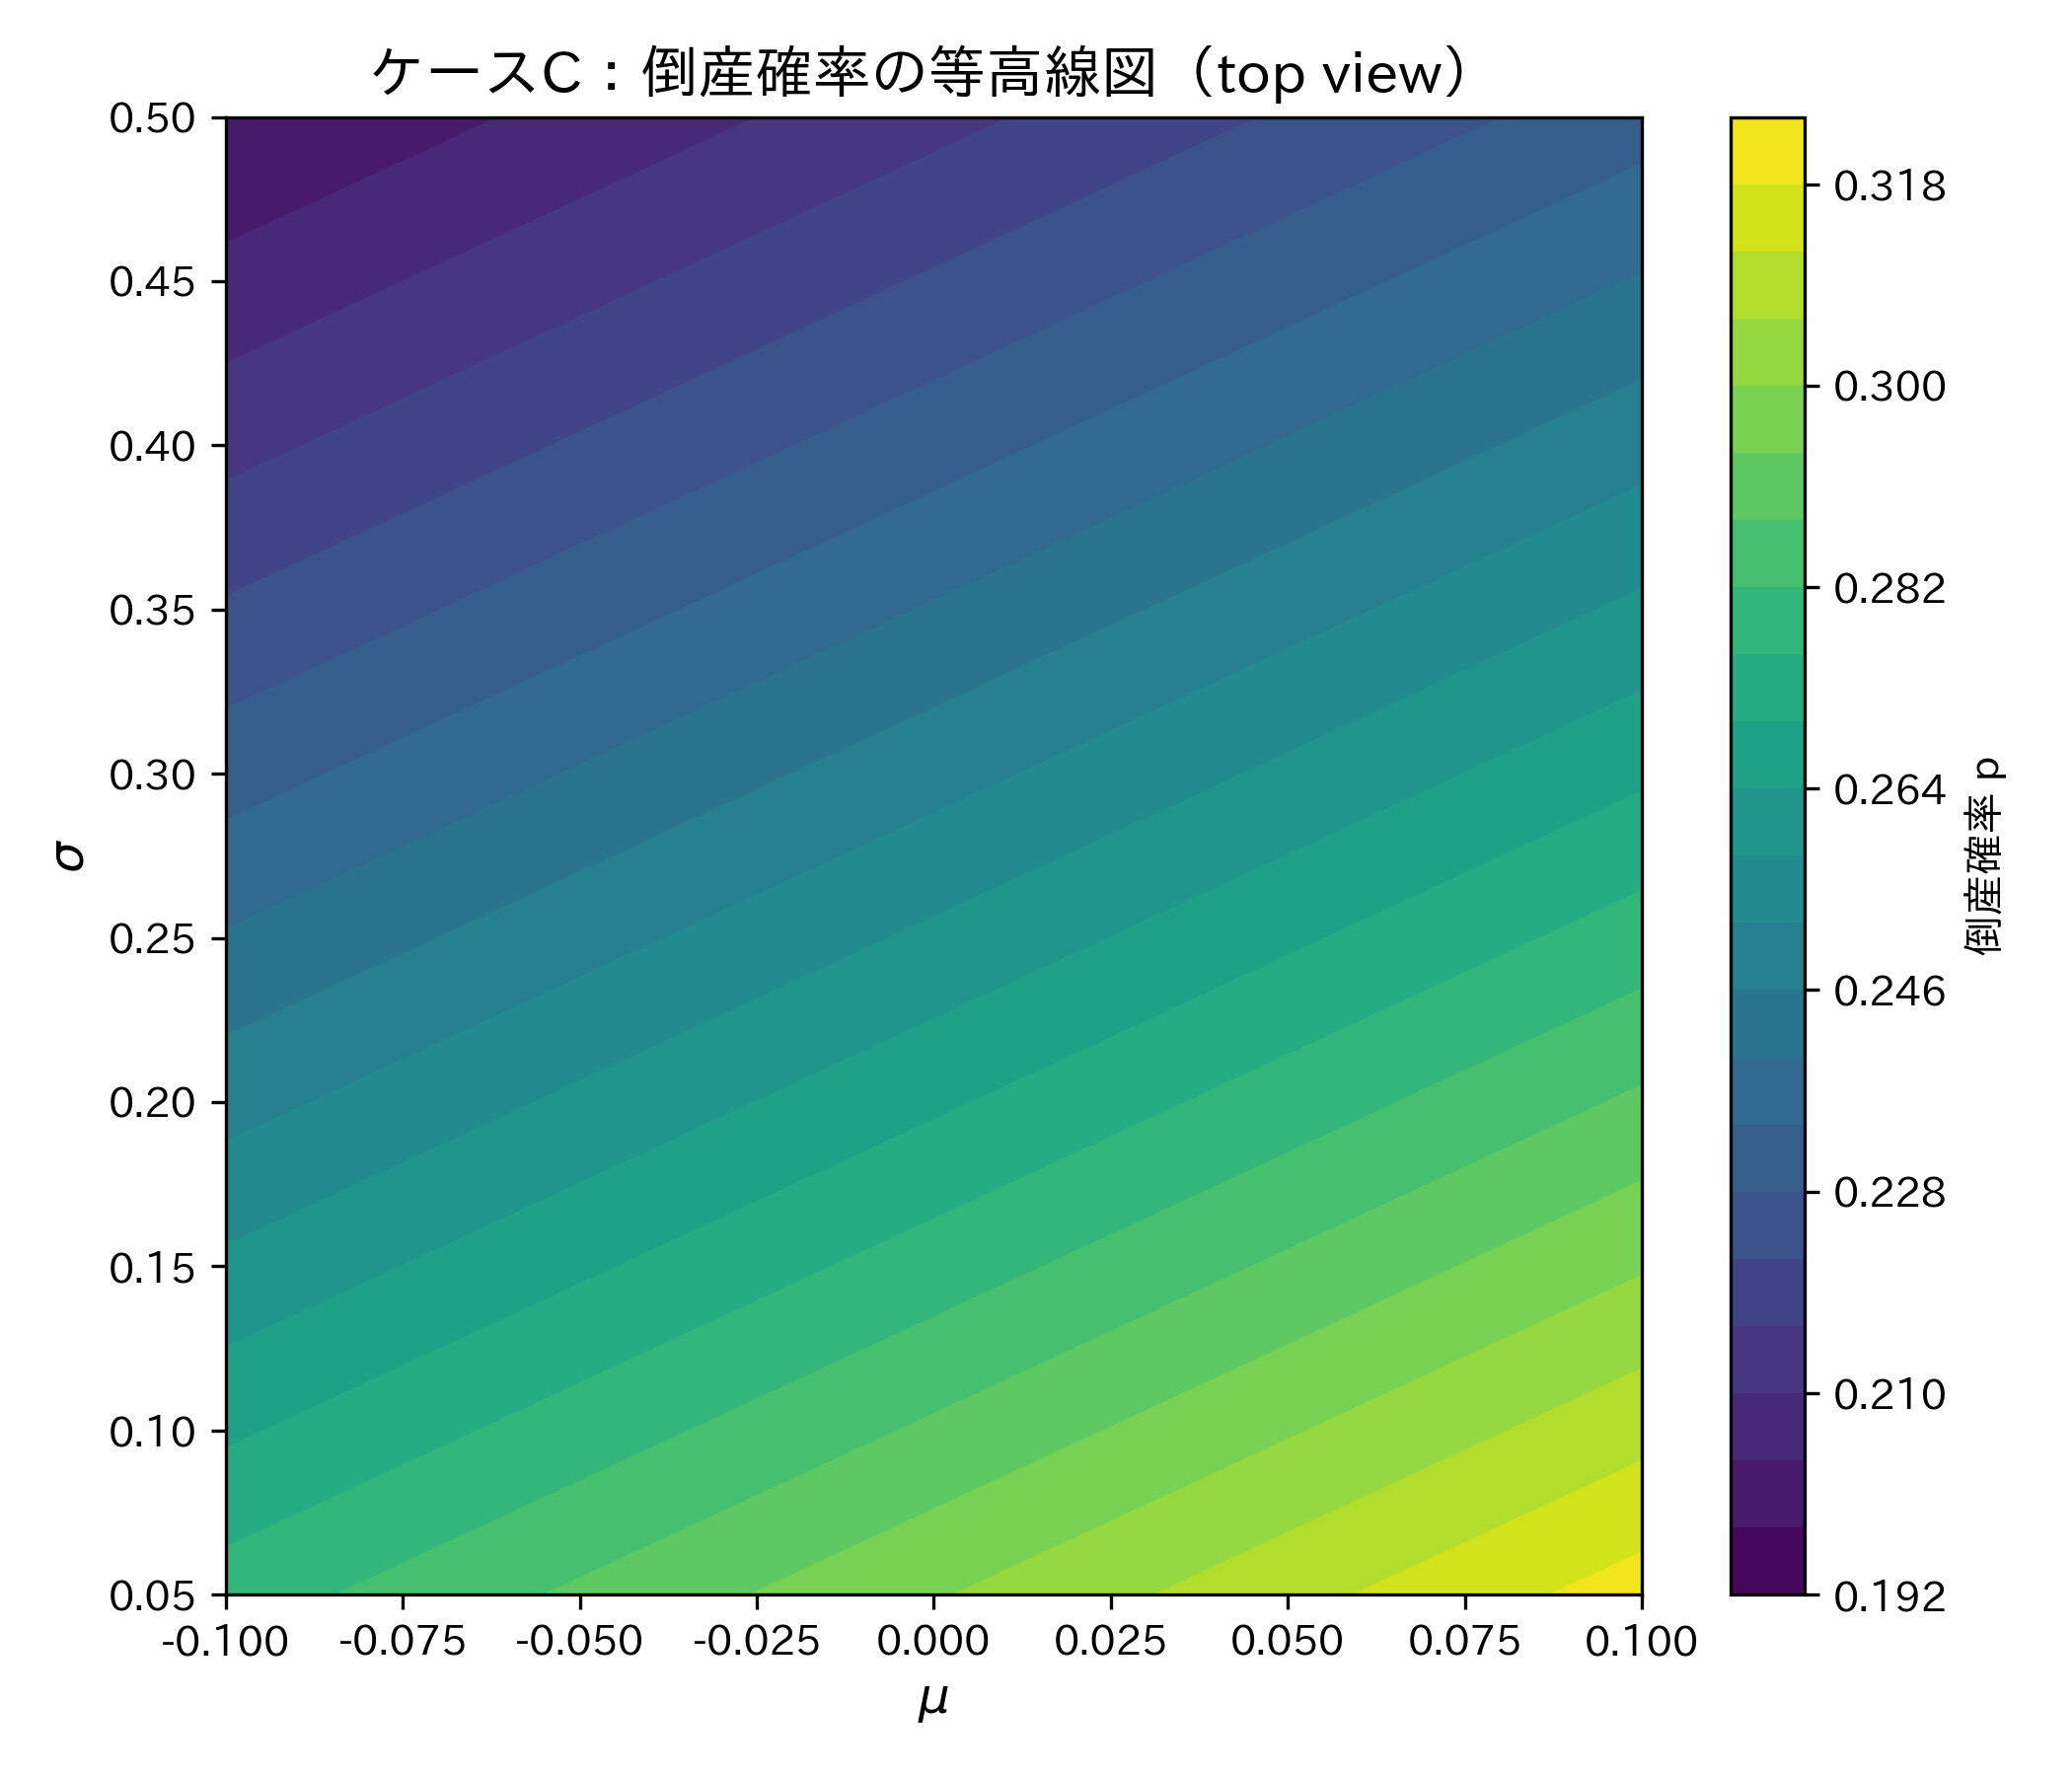
\includegraphics[width=0.75\linewidth]{figures/contour_caseC.png}
    \caption{ケースC（$D=0.8,\ S=0$）：倒産確率の等高線図。
    負債過多により境界線が大きく左へ寄り，
    高ボラティリティ環境で極めて脆弱であることが示される。}
\end{figure}

\begin{figure}[H]
    \centering
    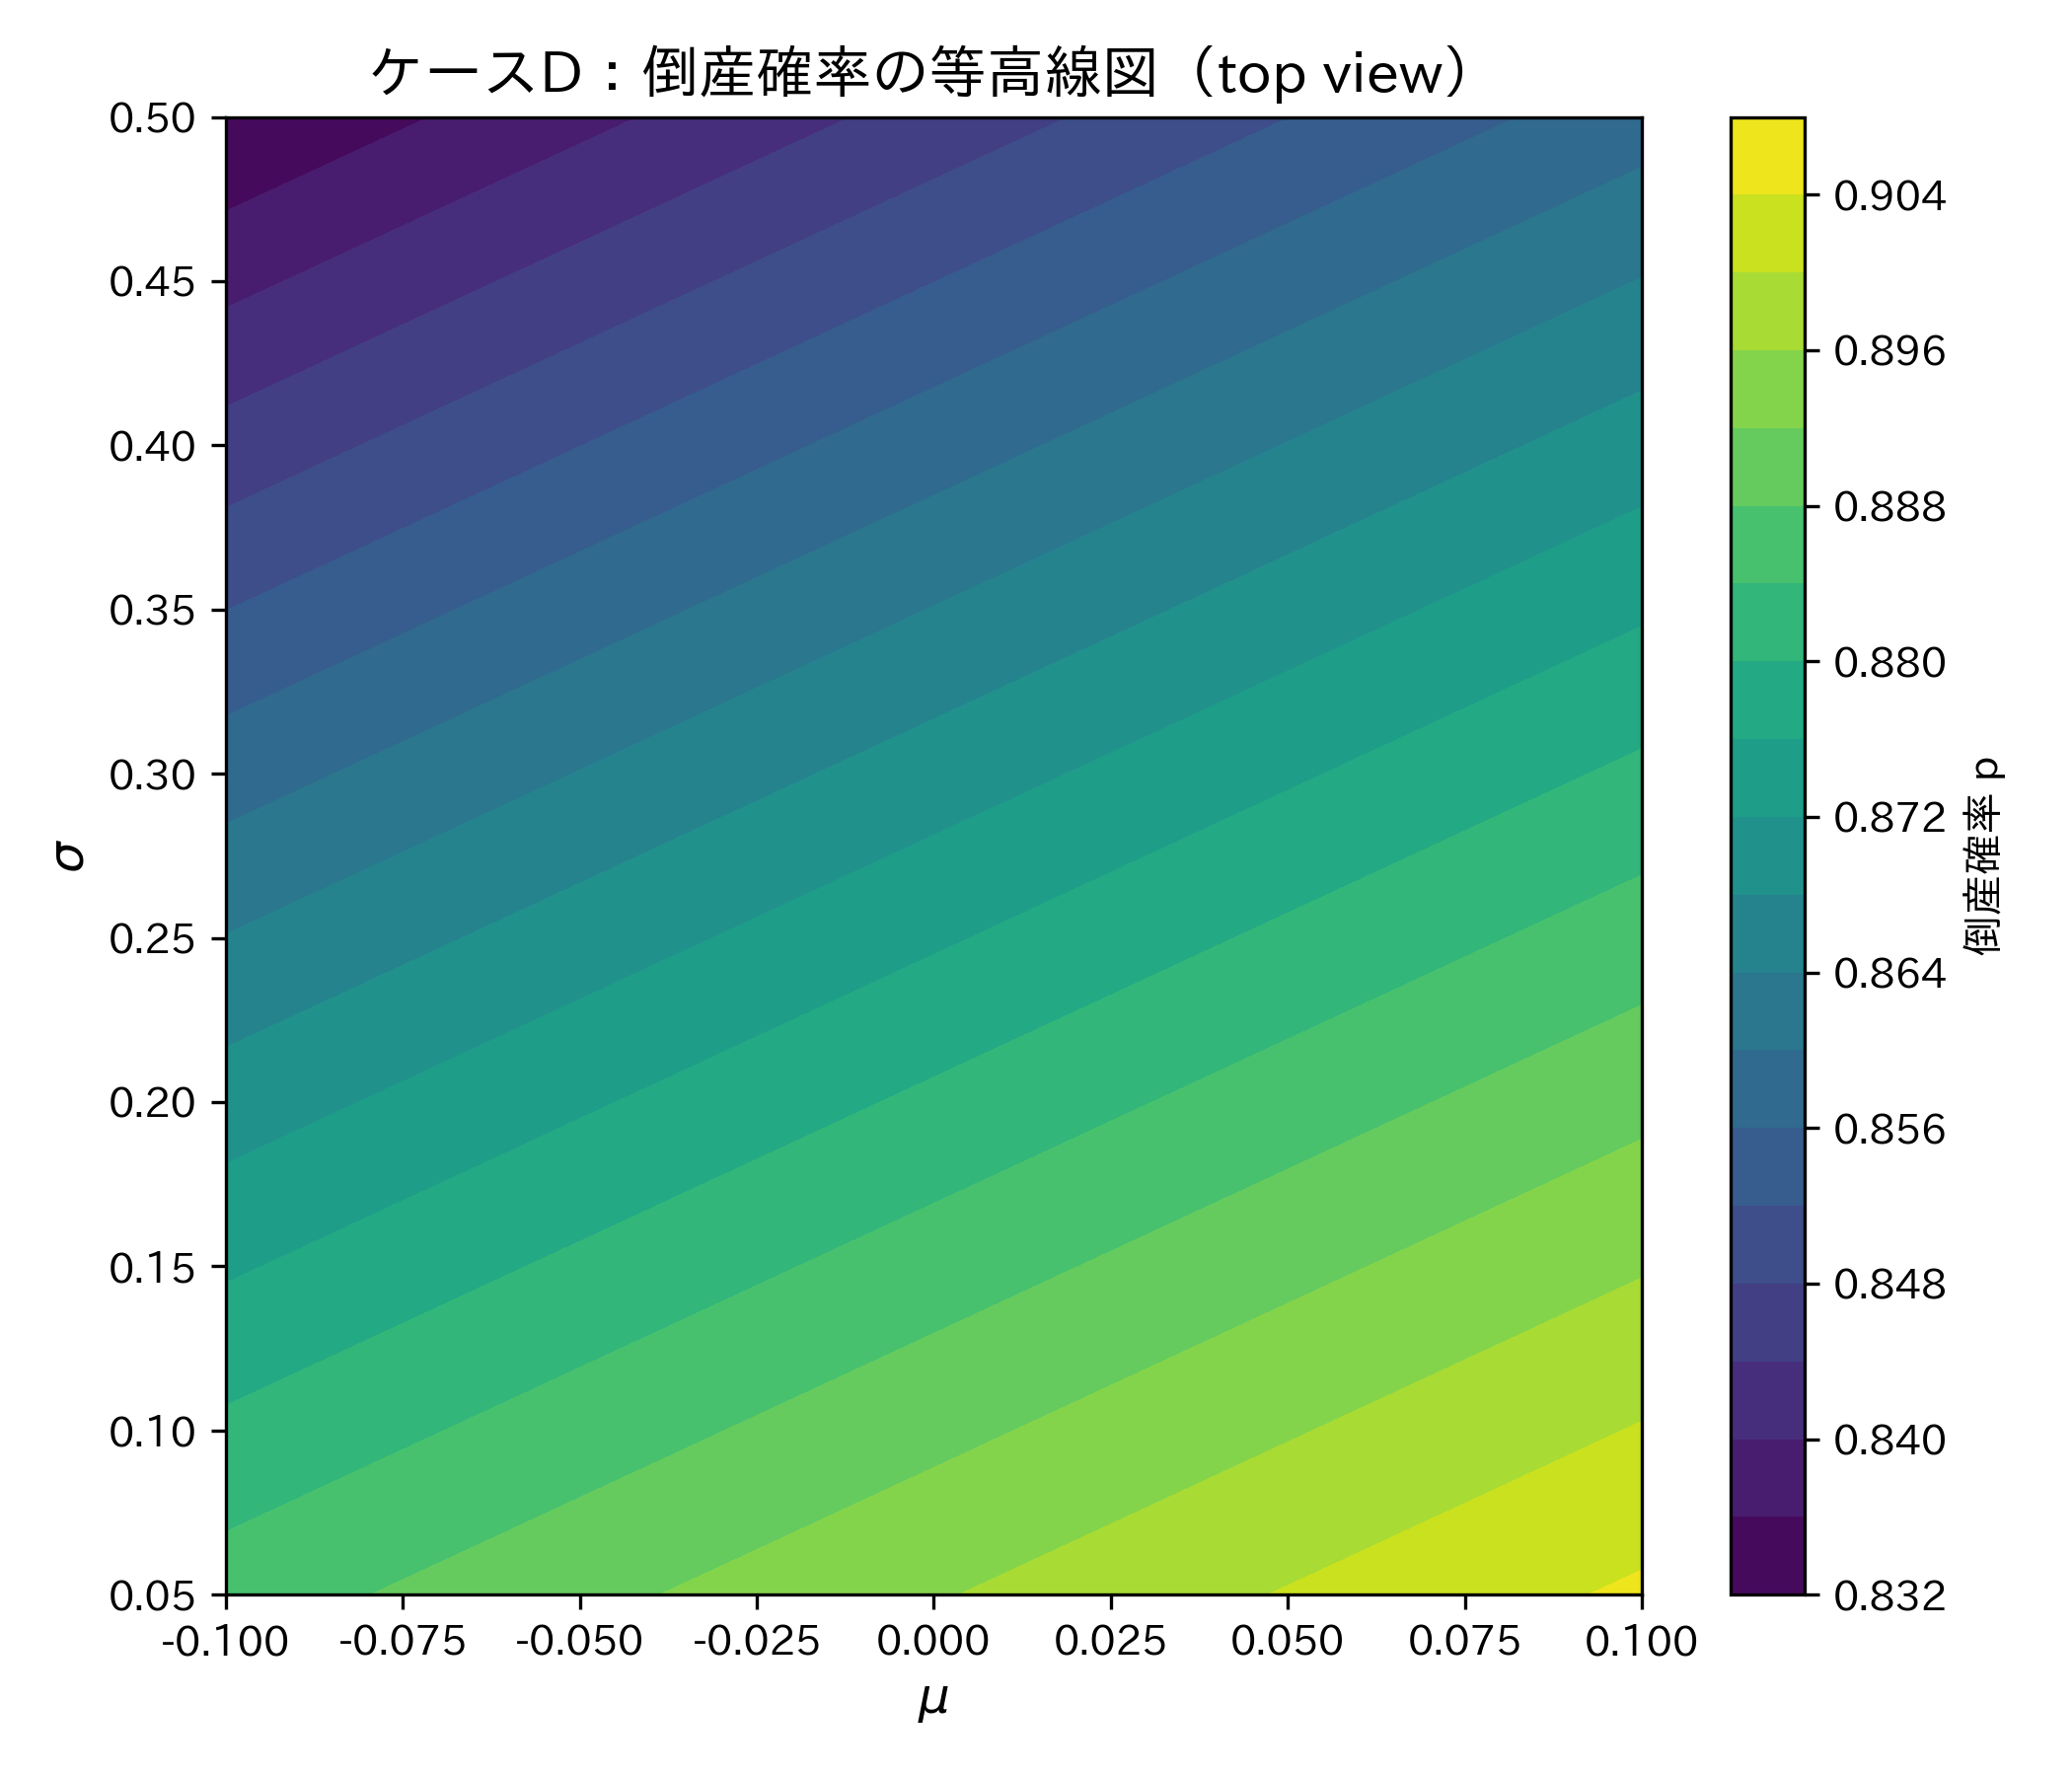
\includegraphics[width=0.75\linewidth]{figures/contour_caseD.png}
    \caption{ケースD（$D=0.8,\ S=3$）：倒産確率の等高線図。
    負債比率は高いが支援能力が強いため，
    ケースCと比べて境界線が右へ戻り，倒産リスクが大幅に緩和されている。}
\end{figure}

\begin{figure}[H]
    \centering
    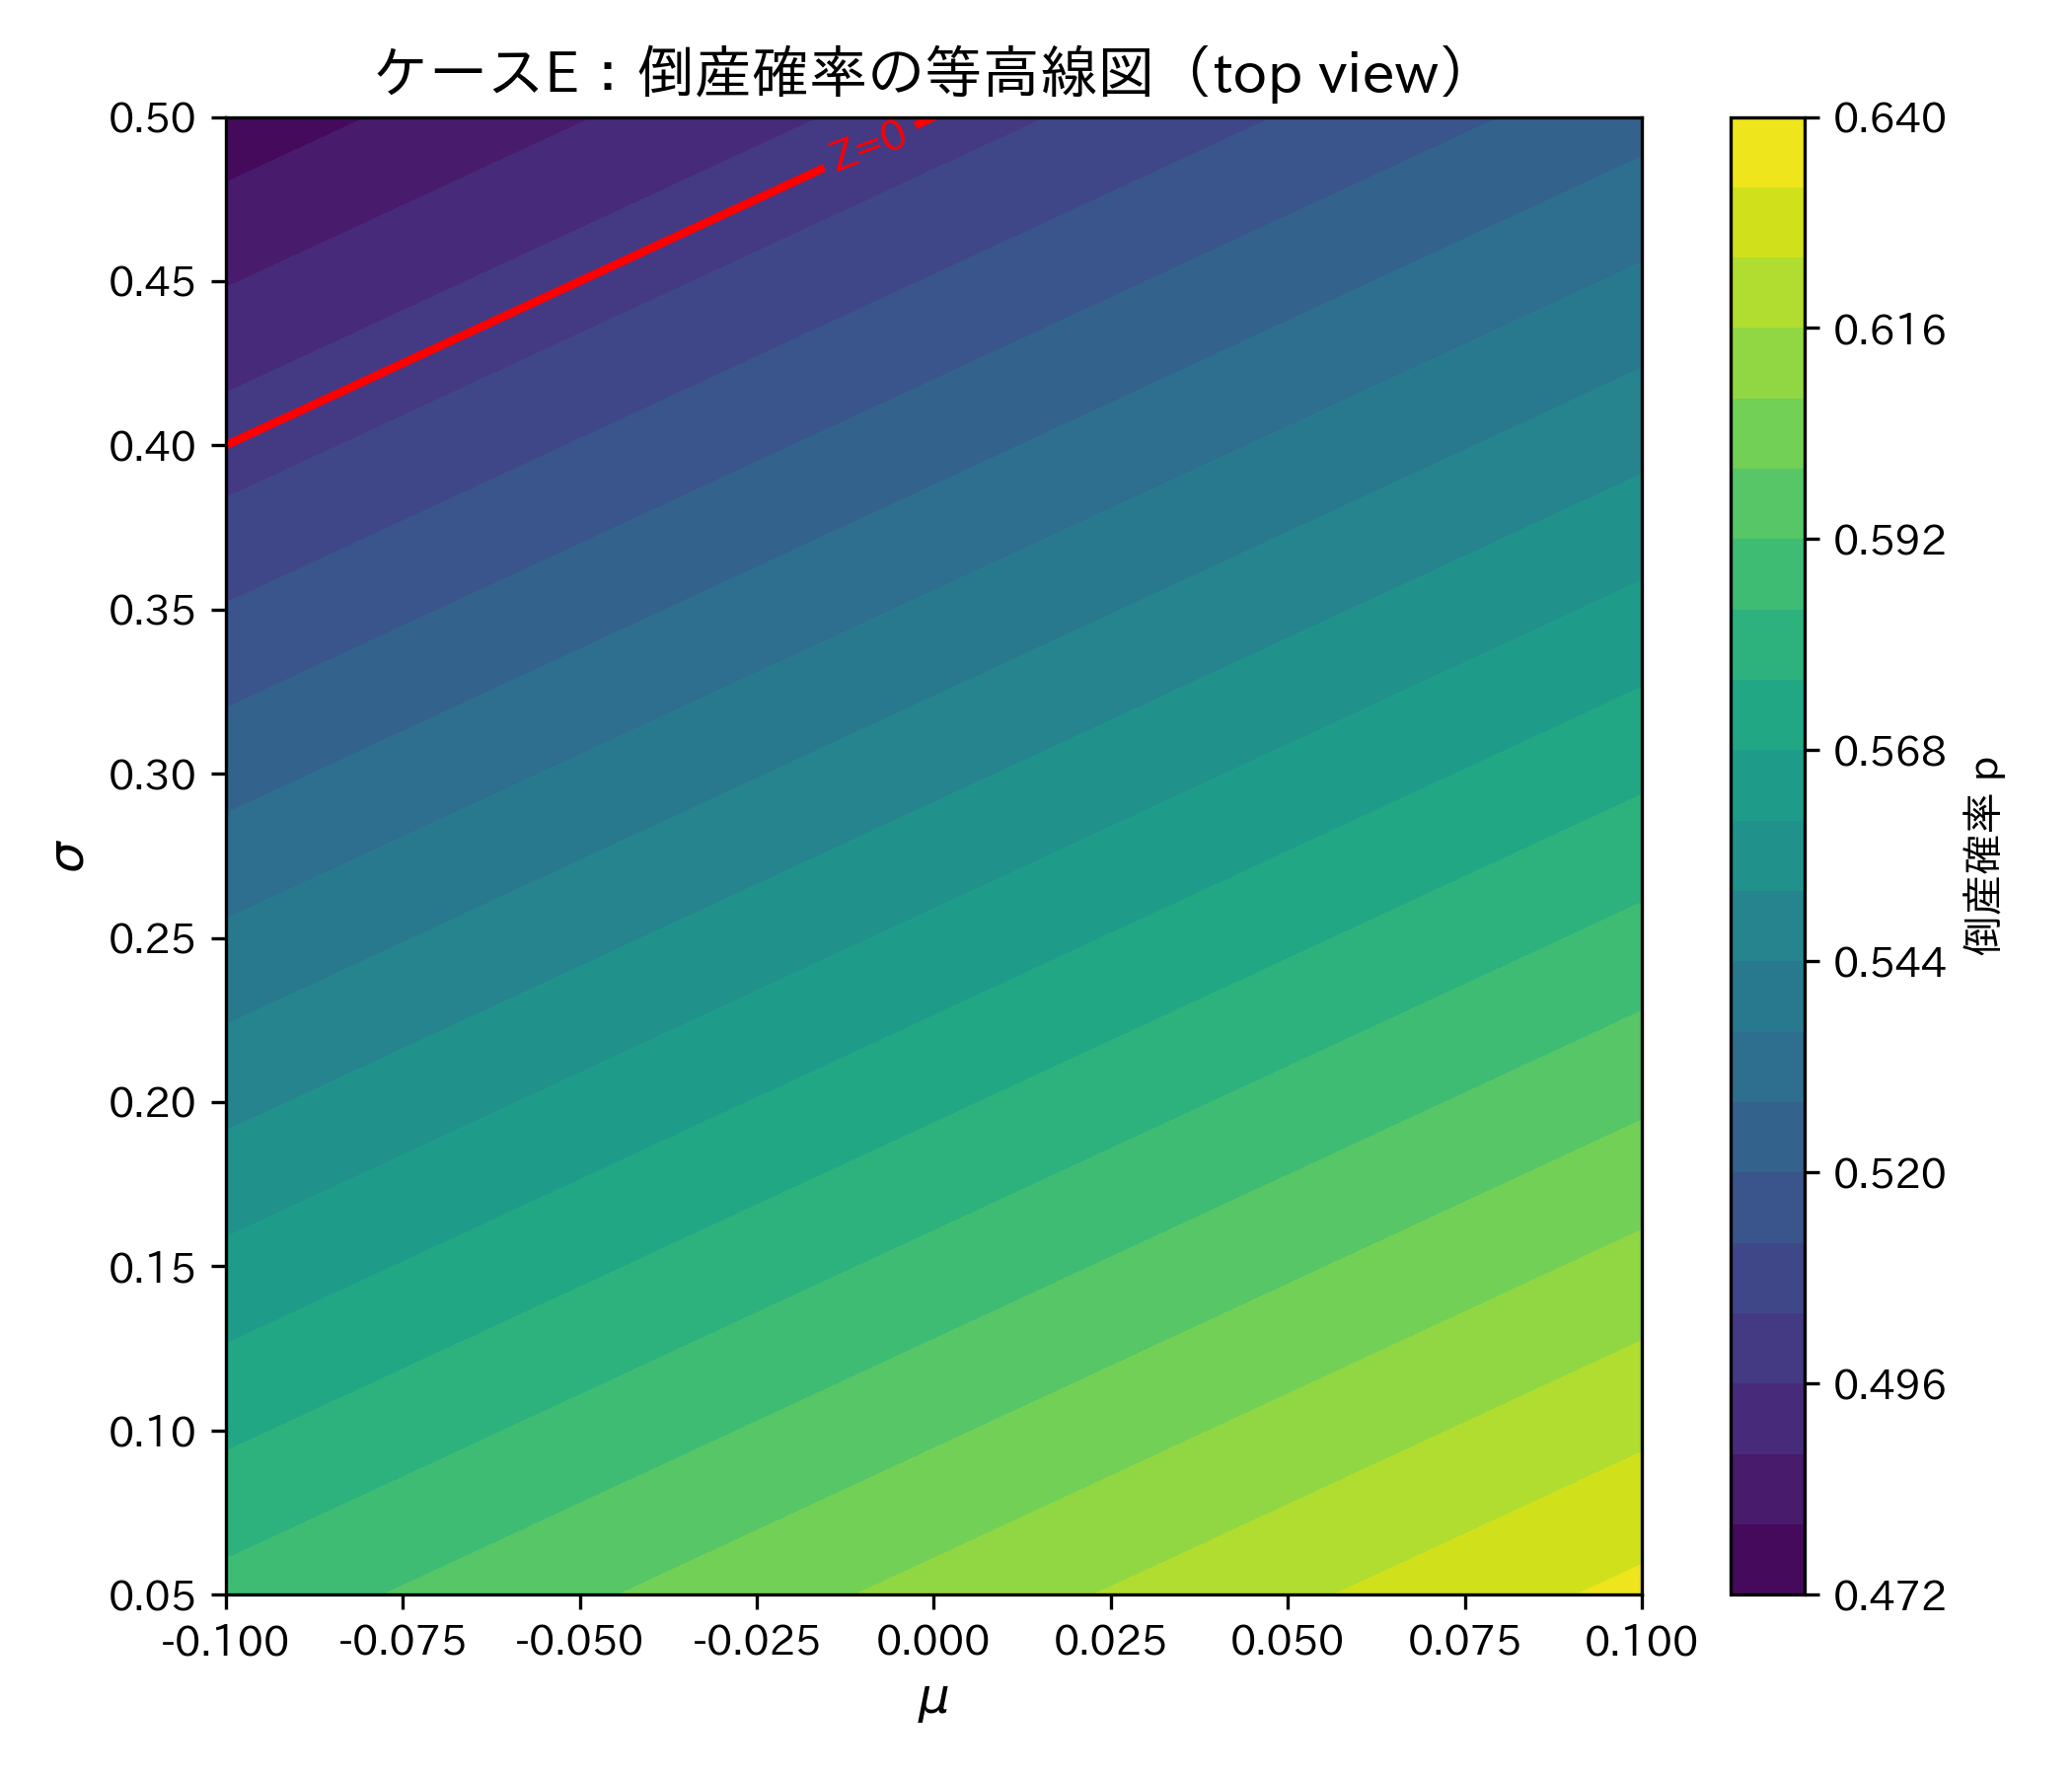
\includegraphics[width=0.75\linewidth]{figures/contour_caseE.png}
    \caption{ケースE（$D=0.5,\ S=1$）：倒産確率の等高線図。
    地域新電力の典型であり，収益性と市場ショックに敏感な構造が確認できる。}
\end{figure}

\begin{figure}[H]
    \centering
    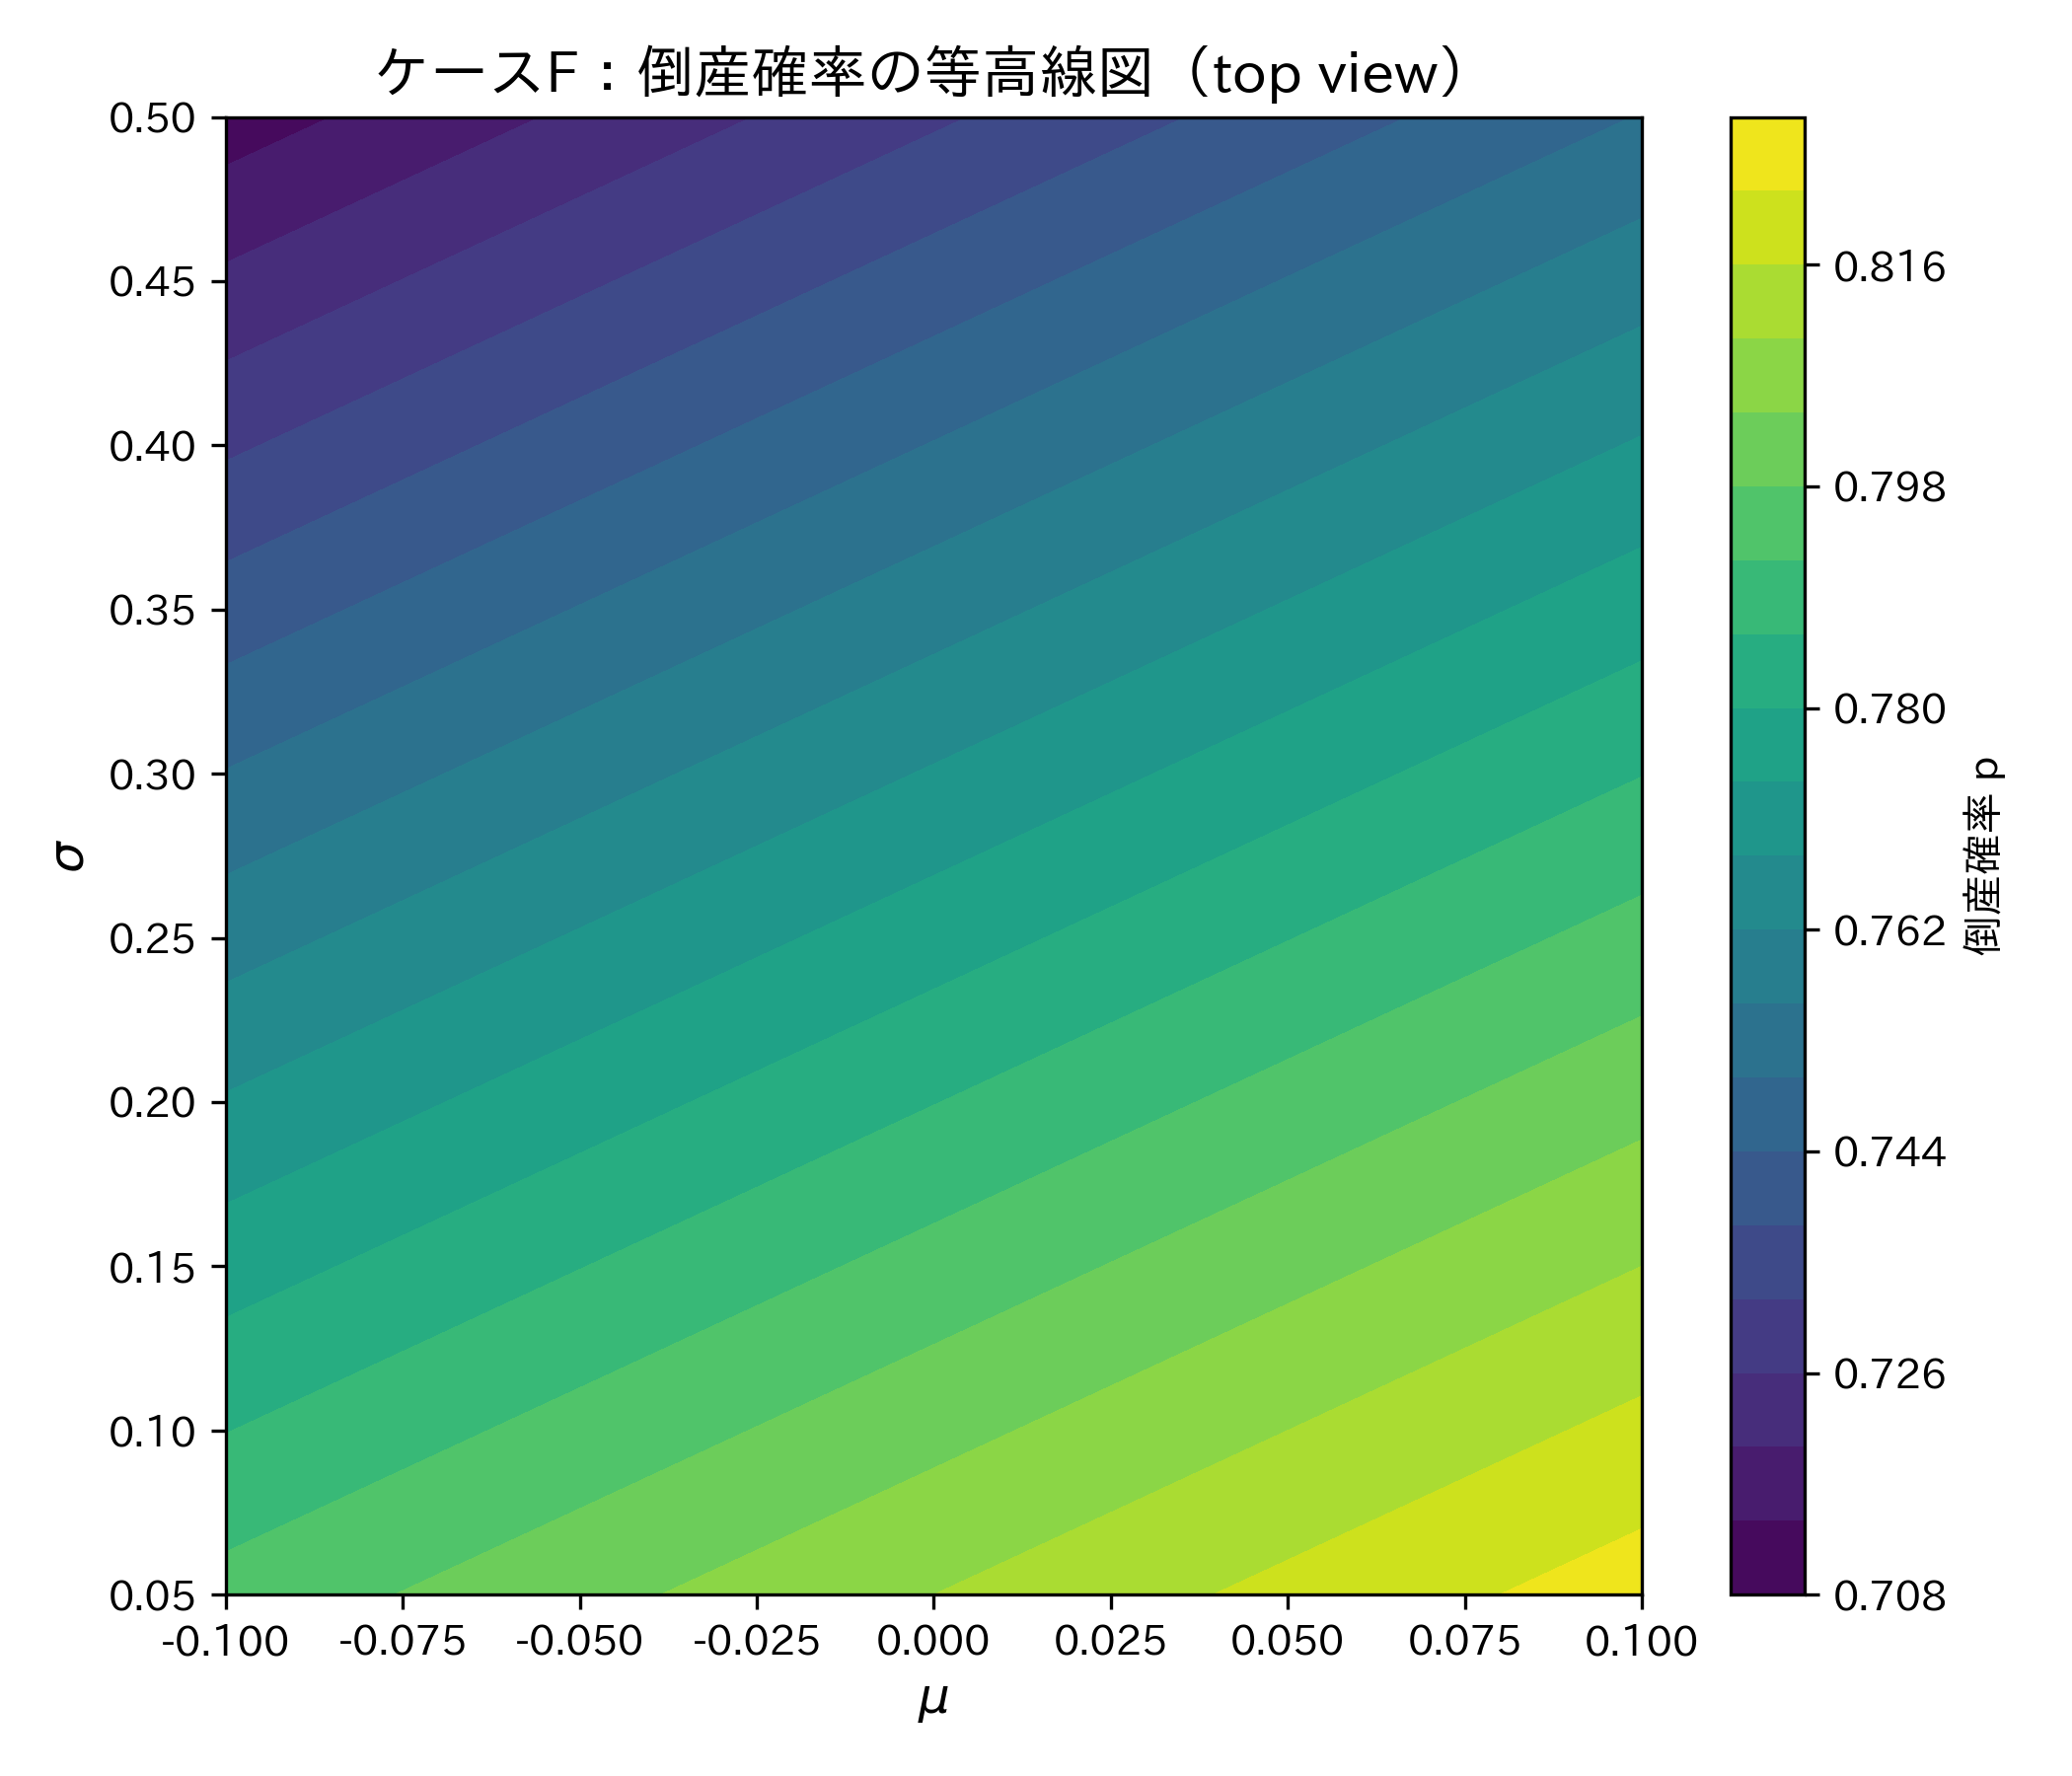
\includegraphics[width=0.75\linewidth]{figures/contour_caseF.png}
    \caption{ケースF（$D=0.5,\ S=2$）：倒産確率の等高線図。
    ケースEと比べて境界線が右へ移動し，
    支援能力の差が倒産リスクを大きく左右することが視覚的に示される。}
\end{figure}

% ------------------------------------------------------------
\section*{C.2 差分図（B−C および F−E）}
\addcontentsline{toc}{section}{C.2 差分図（B−C および F−E）}

本節では，構造的に意味のある 2 組の比較について，
倒産確率の差分 $\Delta p$ を可視化する。
差分図は，支援能力 $S$ と負債比率 $D$ の違いが
倒産確率にどの程度の差を生むかを定量的に示すものである。

\subsection*{C.2.1 大企業 vs 地方電力（ケースB − ケースC）}


\[
\Delta p = p_{\mathrm{B}} - p_{\mathrm{C}}
\]



\begin{figure}[H]
    \centering
    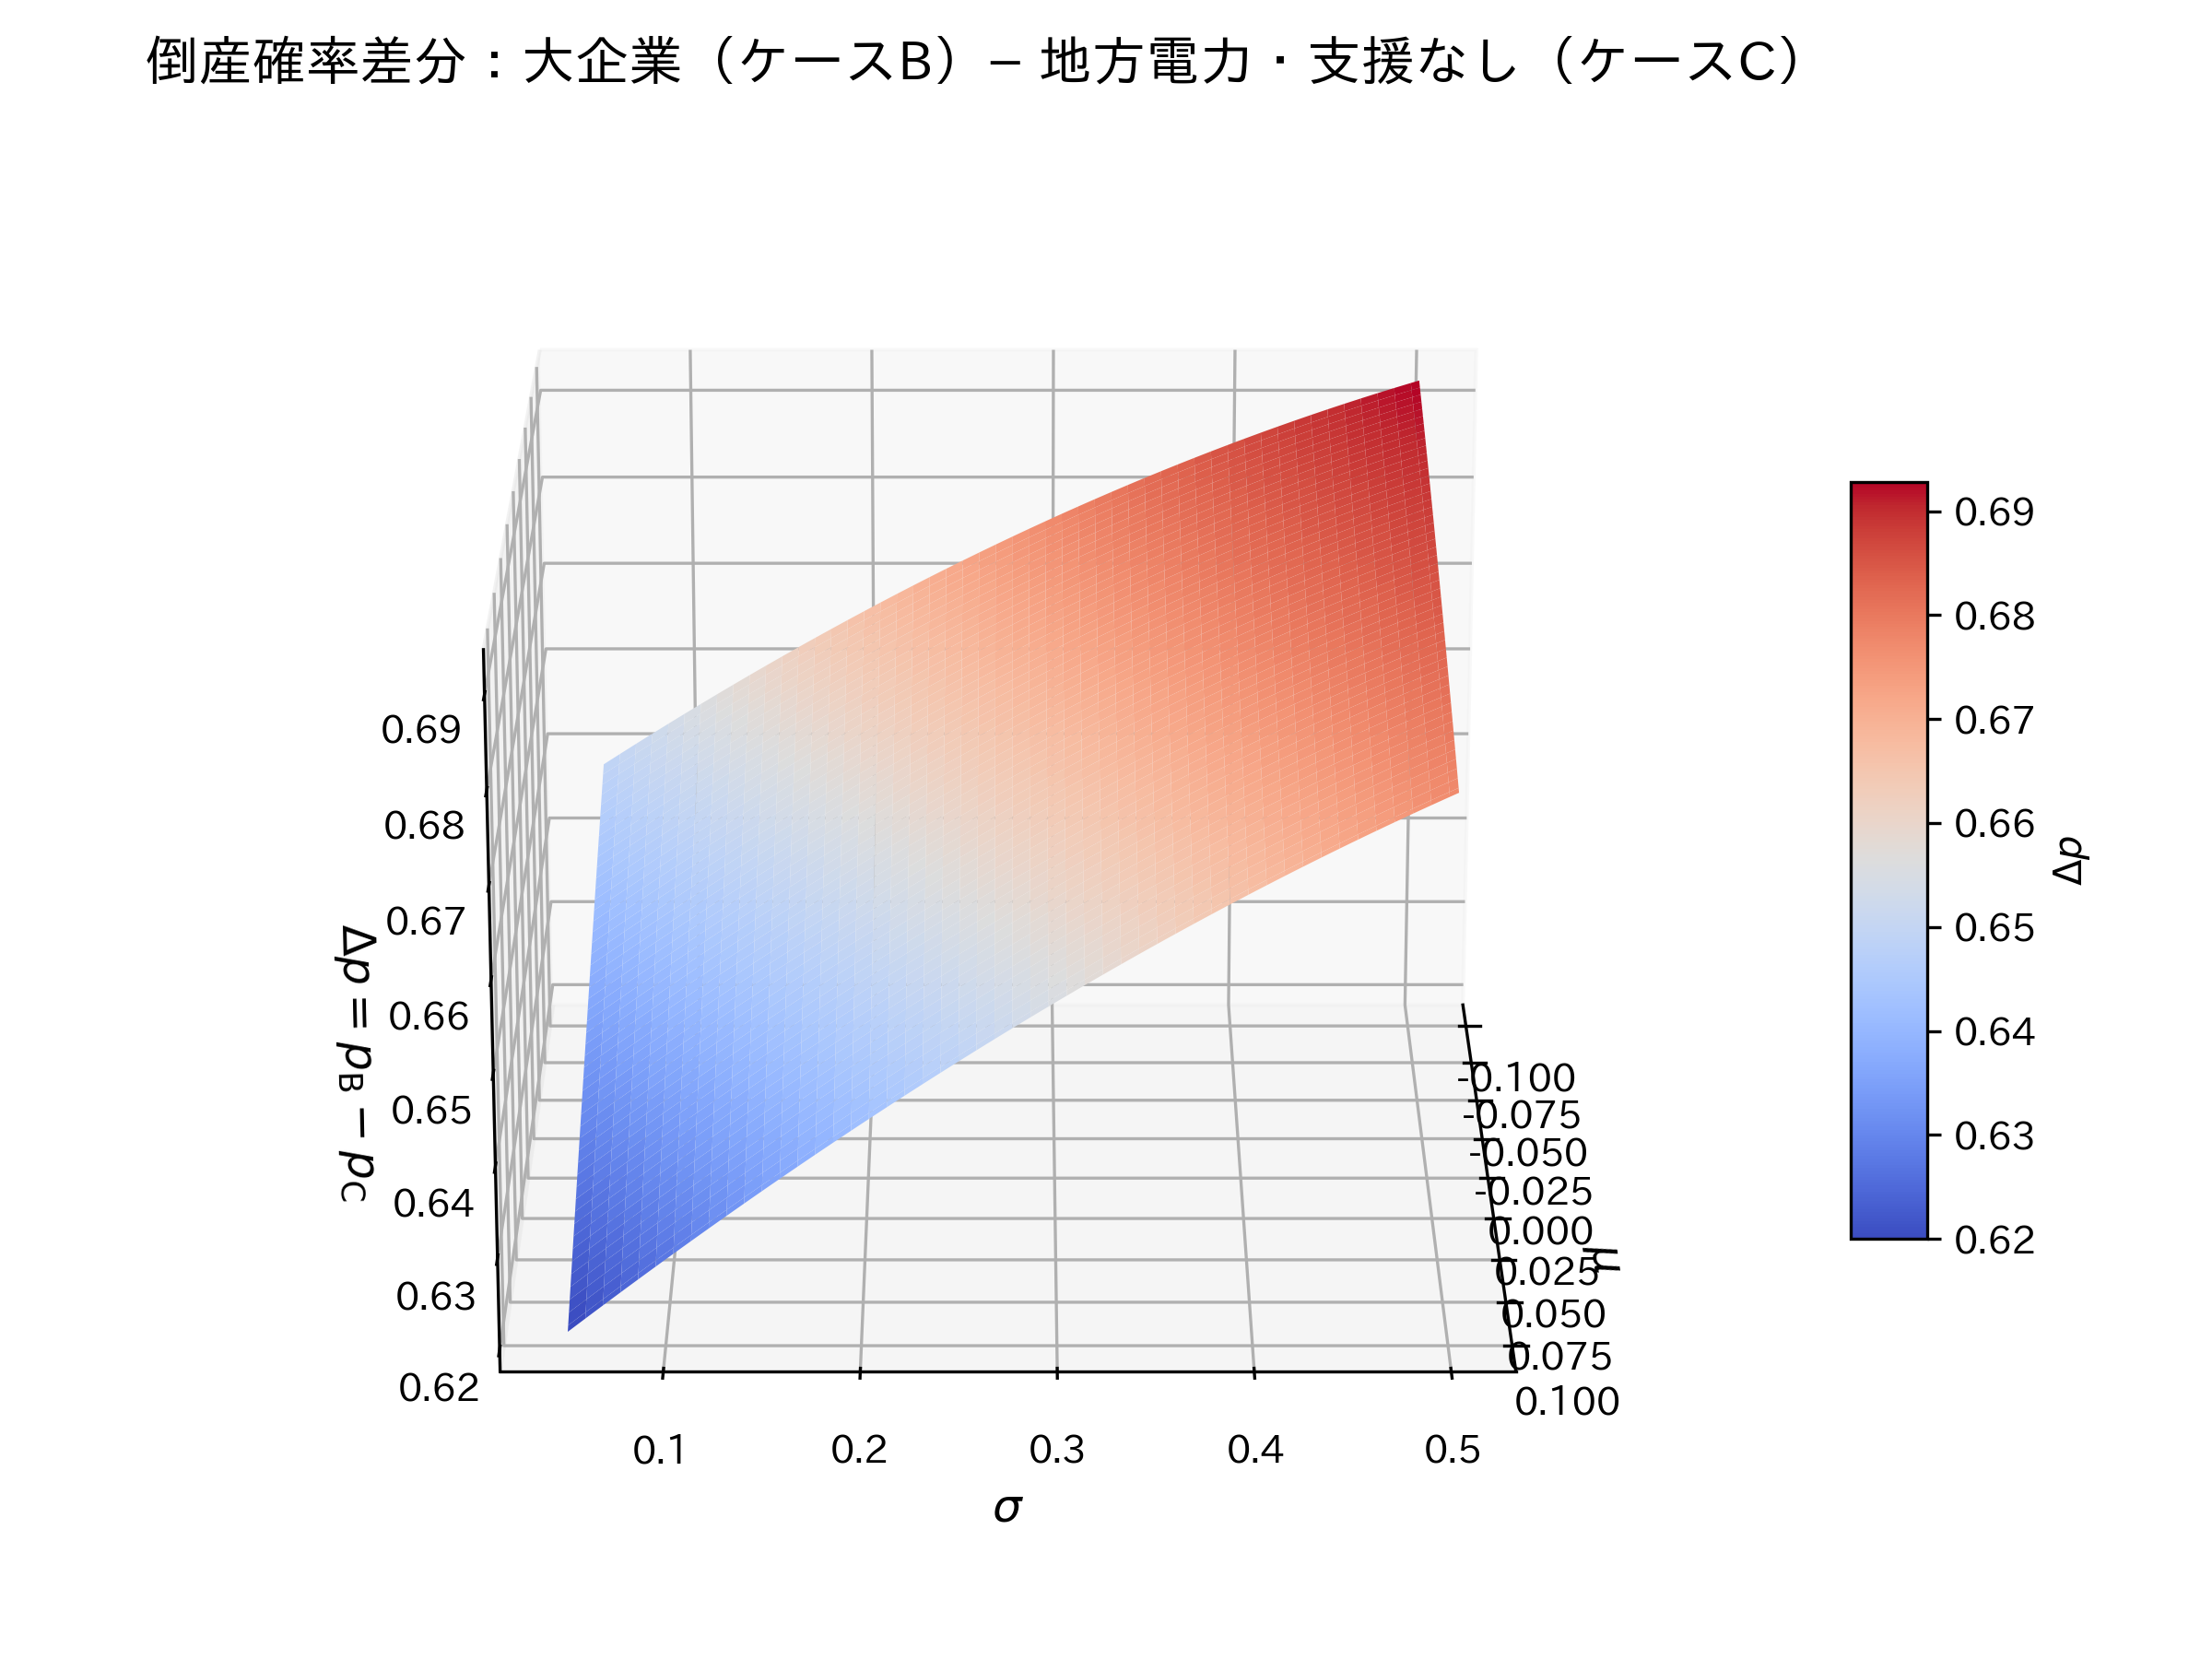
\includegraphics[width=0.75\linewidth]{figures/surface_diff_B_minus_C.png}
    \caption{倒産確率差分：大企業（ケースB）$-$ 地方電力（ケースC）。
    全域で $\Delta p > 0$ となり，支援能力の有無が倒産確率に
    決定的な差を生むことが確認できる。}
\end{figure}

\subsection*{C.2.2 商社系 vs 地域新電力（ケースF − ケースE）}


\[
\Delta p = p_{\mathrm{F}} - p_{\mathrm{E}}
\]



\begin{figure}[H]
    \centering
    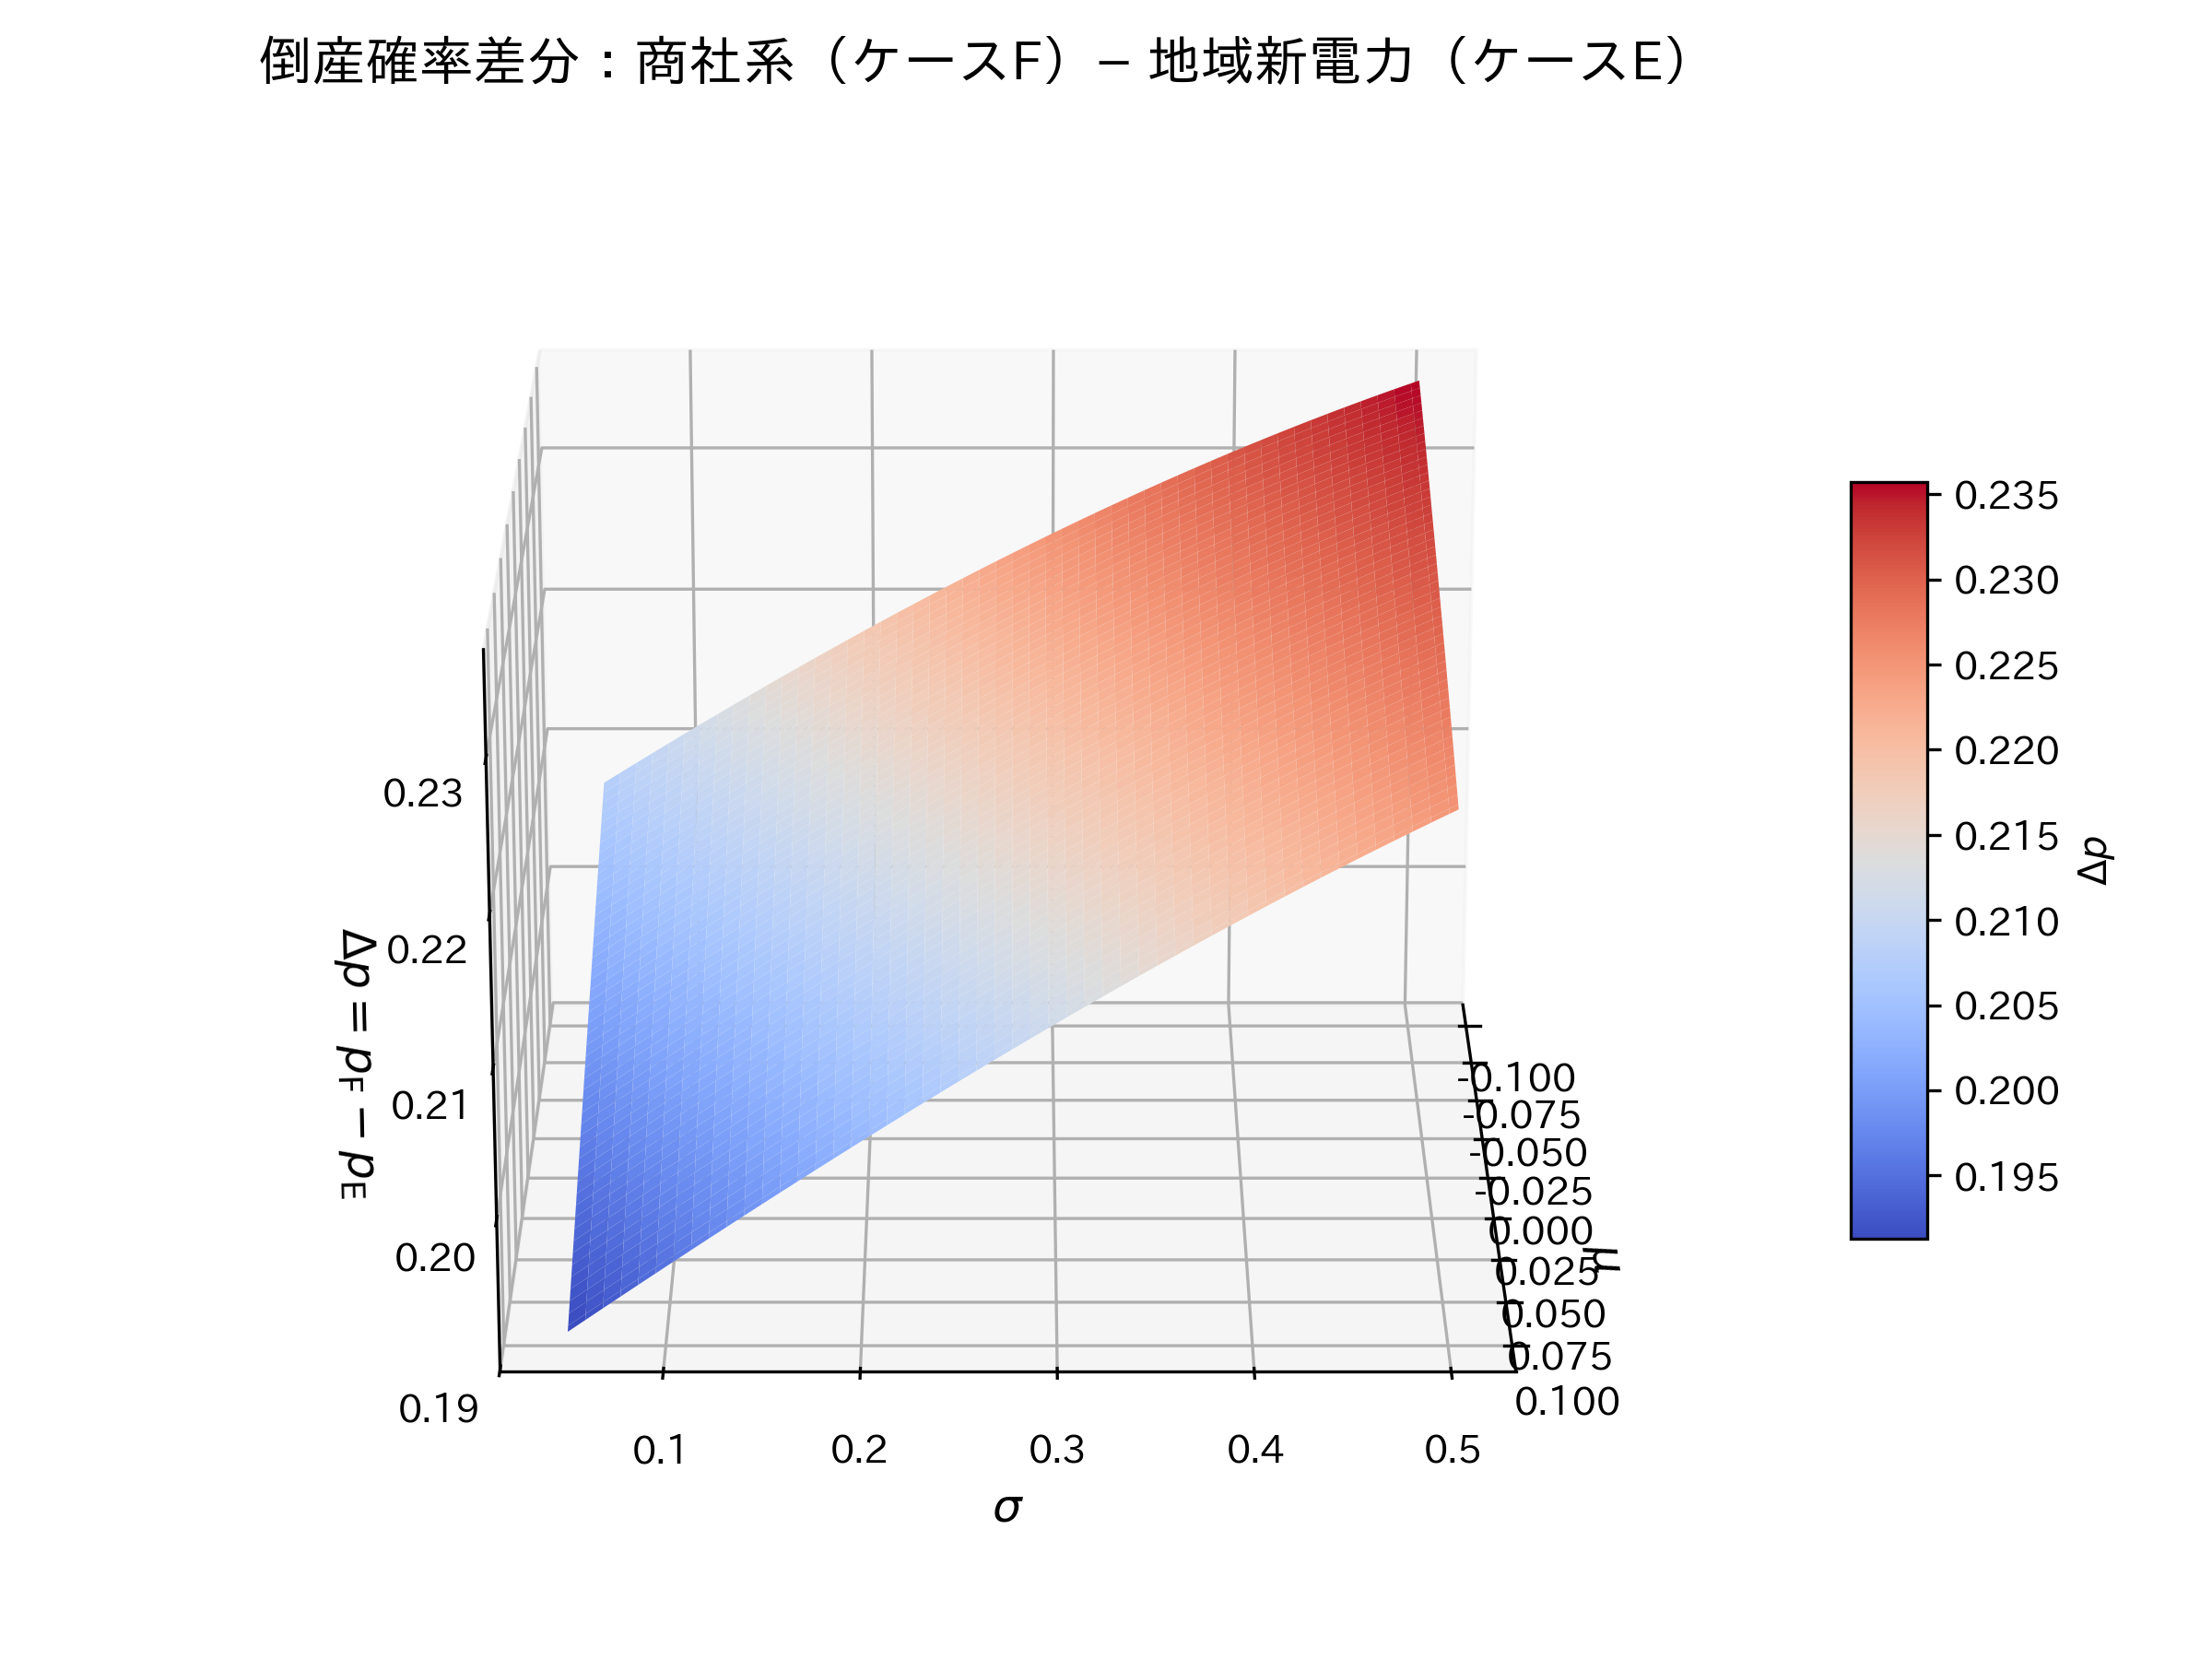
\includegraphics[width=0.75\linewidth]{figures/surface_diff_F_minus_E.png}
    \caption{倒産確率差分：商社系（ケースF）$-$ 地域新電力（ケースE）。
    支援能力 $S$ の差が倒産確率に 0.2〜0.3 程度の差を生み，
    特に $\sigma$ が大きい領域でその効果が最大化する。}
\end{figure}

以上の差分図は，第6章で議論したとおり，
支援能力 $S$ および負債比率 $D$ が倒産確率に与える影響を
視覚的かつ定量的に示すものである。
特に，ケースF−E の比較は，
中規模企業における支援能力の重要性を明確に示している。

% ============================================================
% 付録D B&S 推定式に基づく proxy 妥当性シミュレーション
% ------------------------------------------------------------
% ・第5章で定義した proxy（μ, σ, S, D）がどの程度「真の構造」を回収できるかを検証
% ・理論モデル（真の世界）→ proxy（観測世界）→ B&S 型ロジット推定 の流れを再現
% ・第7章の実証分析に向けた proxy 妥当性の理論的裏付けを与える
% ============================================================

\chapter*{付録 D：B\&S 推定式に基づく proxy 妥当性シミュレーション}
\label{app:bs_simulation}
\addcontentsline{toc}{chapter}{付録 D：B\&S 推定式に基づく proxy 妥当性シミュレーション}

\section*{D.1　分析の目的と概要}
\addcontentsline{toc}{section}{D.1　分析の目的と概要}

本節では，第5章で定義した収益性 $\mu$，市場ショック $\sigma$，
支援能力 $S$，倒産閾値 $D$ の各 proxy が，
理論モデルの「真の構造」をどの程度回収できるかを検証するため，
Bharath and Shumway（2008）（以下 B\&S）の推定式に基づく
シミュレーション分析を行う。

本分析の目的は，実証データが限定的な新電力企業において，
proxy 変数を用いたロジット推定がどの程度信頼できるかを
理論的に裏付けることである。

% ------------------------------------------------------------
\subsection*{D.1.1　分析の基本構造：真の世界と観測世界}

本シミュレーションは，以下の 3 段階で構成される。

\begin{enumerate}
    \item \textbf{真の世界（理論モデル）}  
    第4章で導出した潜在倒産距離
    


\[
        Z^{\ast}_i = a \mu^{\ast}_i - b \sigma^{\ast}_i + c S^{\ast}_i - d D^{\ast}_i
    \]



    を用いて，真の倒産確率
    


\[
        p_i = \frac{1}{1 + \exp(-Z^{\ast}_i)}
    \]



    を生成し，倒産ダミー $\text{Default}_i$ を発生させる。

    \item \textbf{観測世界（proxy の生成）}  
    真のパラメータ $\mu^{\ast}, \sigma^{\ast}, S^{\ast}, D^{\ast}$ から，
    第5章で定義した観測可能な proxy を生成する。

    \item \textbf{B\&S 型ロジット推定}  
    観測 proxy を説明変数としてロジット推定を行い，
    真の係数 $(a,b,c,d)$ をどの程度回収できるかを比較する。
\end{enumerate}

% ------------------------------------------------------------
\subsection*{D.1.2　真のパラメータの設定}

真のパラメータは以下のように設定する。



\[
\mu^{\ast}_i \sim N(0.02, 0.03^2), \qquad
\sigma^{\ast}_i \sim N(0.20, 0.05^2)
\]





\[
S^{\ast}_i \in \{0,1,2,3\}, \qquad
D^{\ast}_i \sim \mathrm{Lognormal}(-1.0, 0.4^2)
\]



係数は理論モデルの符号条件に基づき，



\[
a = 1.0,\quad b = 1.0,\quad c = 0.8,\quad d = 1.2
\]



とする。

% ------------------------------------------------------------
\subsection*{D.1.3　proxy の生成：観測誤差の導入}

\noindent\textbf{（1）収益性の proxy}



\[
\tilde{\mu}^{(1)}_i = \mu^{\ast}_i + \varepsilon^{(1)}_i
\qquad
\tilde{\mu}^{(2)}_i = 0.8 \mu^{\ast}_i + \varepsilon^{(2)}_i
\]



\noindent\textbf{（2）市場ショックの proxy}



\[
\tilde{\sigma}_i = 0.7 \sigma^{\ast}_i + \eta_i
\]



\noindent\textbf{（3）支援能力の proxy}



\[
\tilde{S}_i =
\begin{cases}
S^{\ast}_i & \text{確率 } 0.9 \\
S^{\ast}_i - 1 & \text{確率 } 0.1
\end{cases}
\]



\noindent\textbf{（4）倒産閾値の proxy}



\[
\tilde{D}_i = D^{\ast}_i + \xi_i
\]



% ------------------------------------------------------------
\subsection*{D.1.4　推定式の仕様：proxy の違いによる比較}

以下の 4 つのロジット仕様を推定し，
真の係数 $(a,b,c,d)$ をどの程度回収できるかを比較する。

\begin{itemize}
    \item 仕様A：理論に最も近い proxy（$\tilde{\mu}^{(1)}, \tilde{\sigma}, \tilde{S}, \tilde{D}$）
    \item 仕様B：$\mu$ を貸借対照表 proxy（$\tilde{\mu}^{(2)}$）に置換
    \item 仕様C：$D$ を粗い proxy に置換
    \item 仕様D：$\mu$ と $D$ の両方を粗い proxy に置換
\end{itemize}

% ------------------------------------------------------------
\subsection*{D.1.5　期待される結果と含意}

本シミュレーションにより，以下が確認されることが期待される。

\begin{enumerate}
    \item 仕様Aが最も真の構造を回収する  
    \item 貸借対照表ベースの $\mu$ proxy は一定の劣化を伴うが符号条件は維持  
    \item 倒産閾値 $D$ の proxy が粗い場合，推定精度が大きく低下  
    \item 支援能力 $S$ は proxy が多少ノイジーでも符号条件を維持しやすい  
\end{enumerate}

以上より，本節のシミュレーションは，
第7章の実証分析における proxy 変数の採用根拠を
理論的に補強する役割を果たす。

% ============================================================
% D.2 B&S 推定式シミュレーション結果の可視化
% ============================================================

\section*{D.2　B\&S 推定式シミュレーション結果の可視化}
\addcontentsline{toc}{section}{D.2　B\&S 推定式シミュレーション結果の可視化}

本節では，前節で実施した B\&S 推定式シミュレーションの結果を可視化し，
proxy 変数の妥当性を視覚的に評価する。
特に，推定係数の比較，ROC 曲線，真の倒産確率と推定確率の散布図を用いて，
各 proxy の性能を体系的に検証する。

% ------------------------------------------------------------
\subsection*{D.2.1　推定係数の比較プロット}

図\ref{fig:coef_comparison} は，真の係数 $(a,b,c,d)$ と，
仕様A〜Dのロジット推定で得られた係数を比較したものである。

\begin{figure}[H]
    \centering
    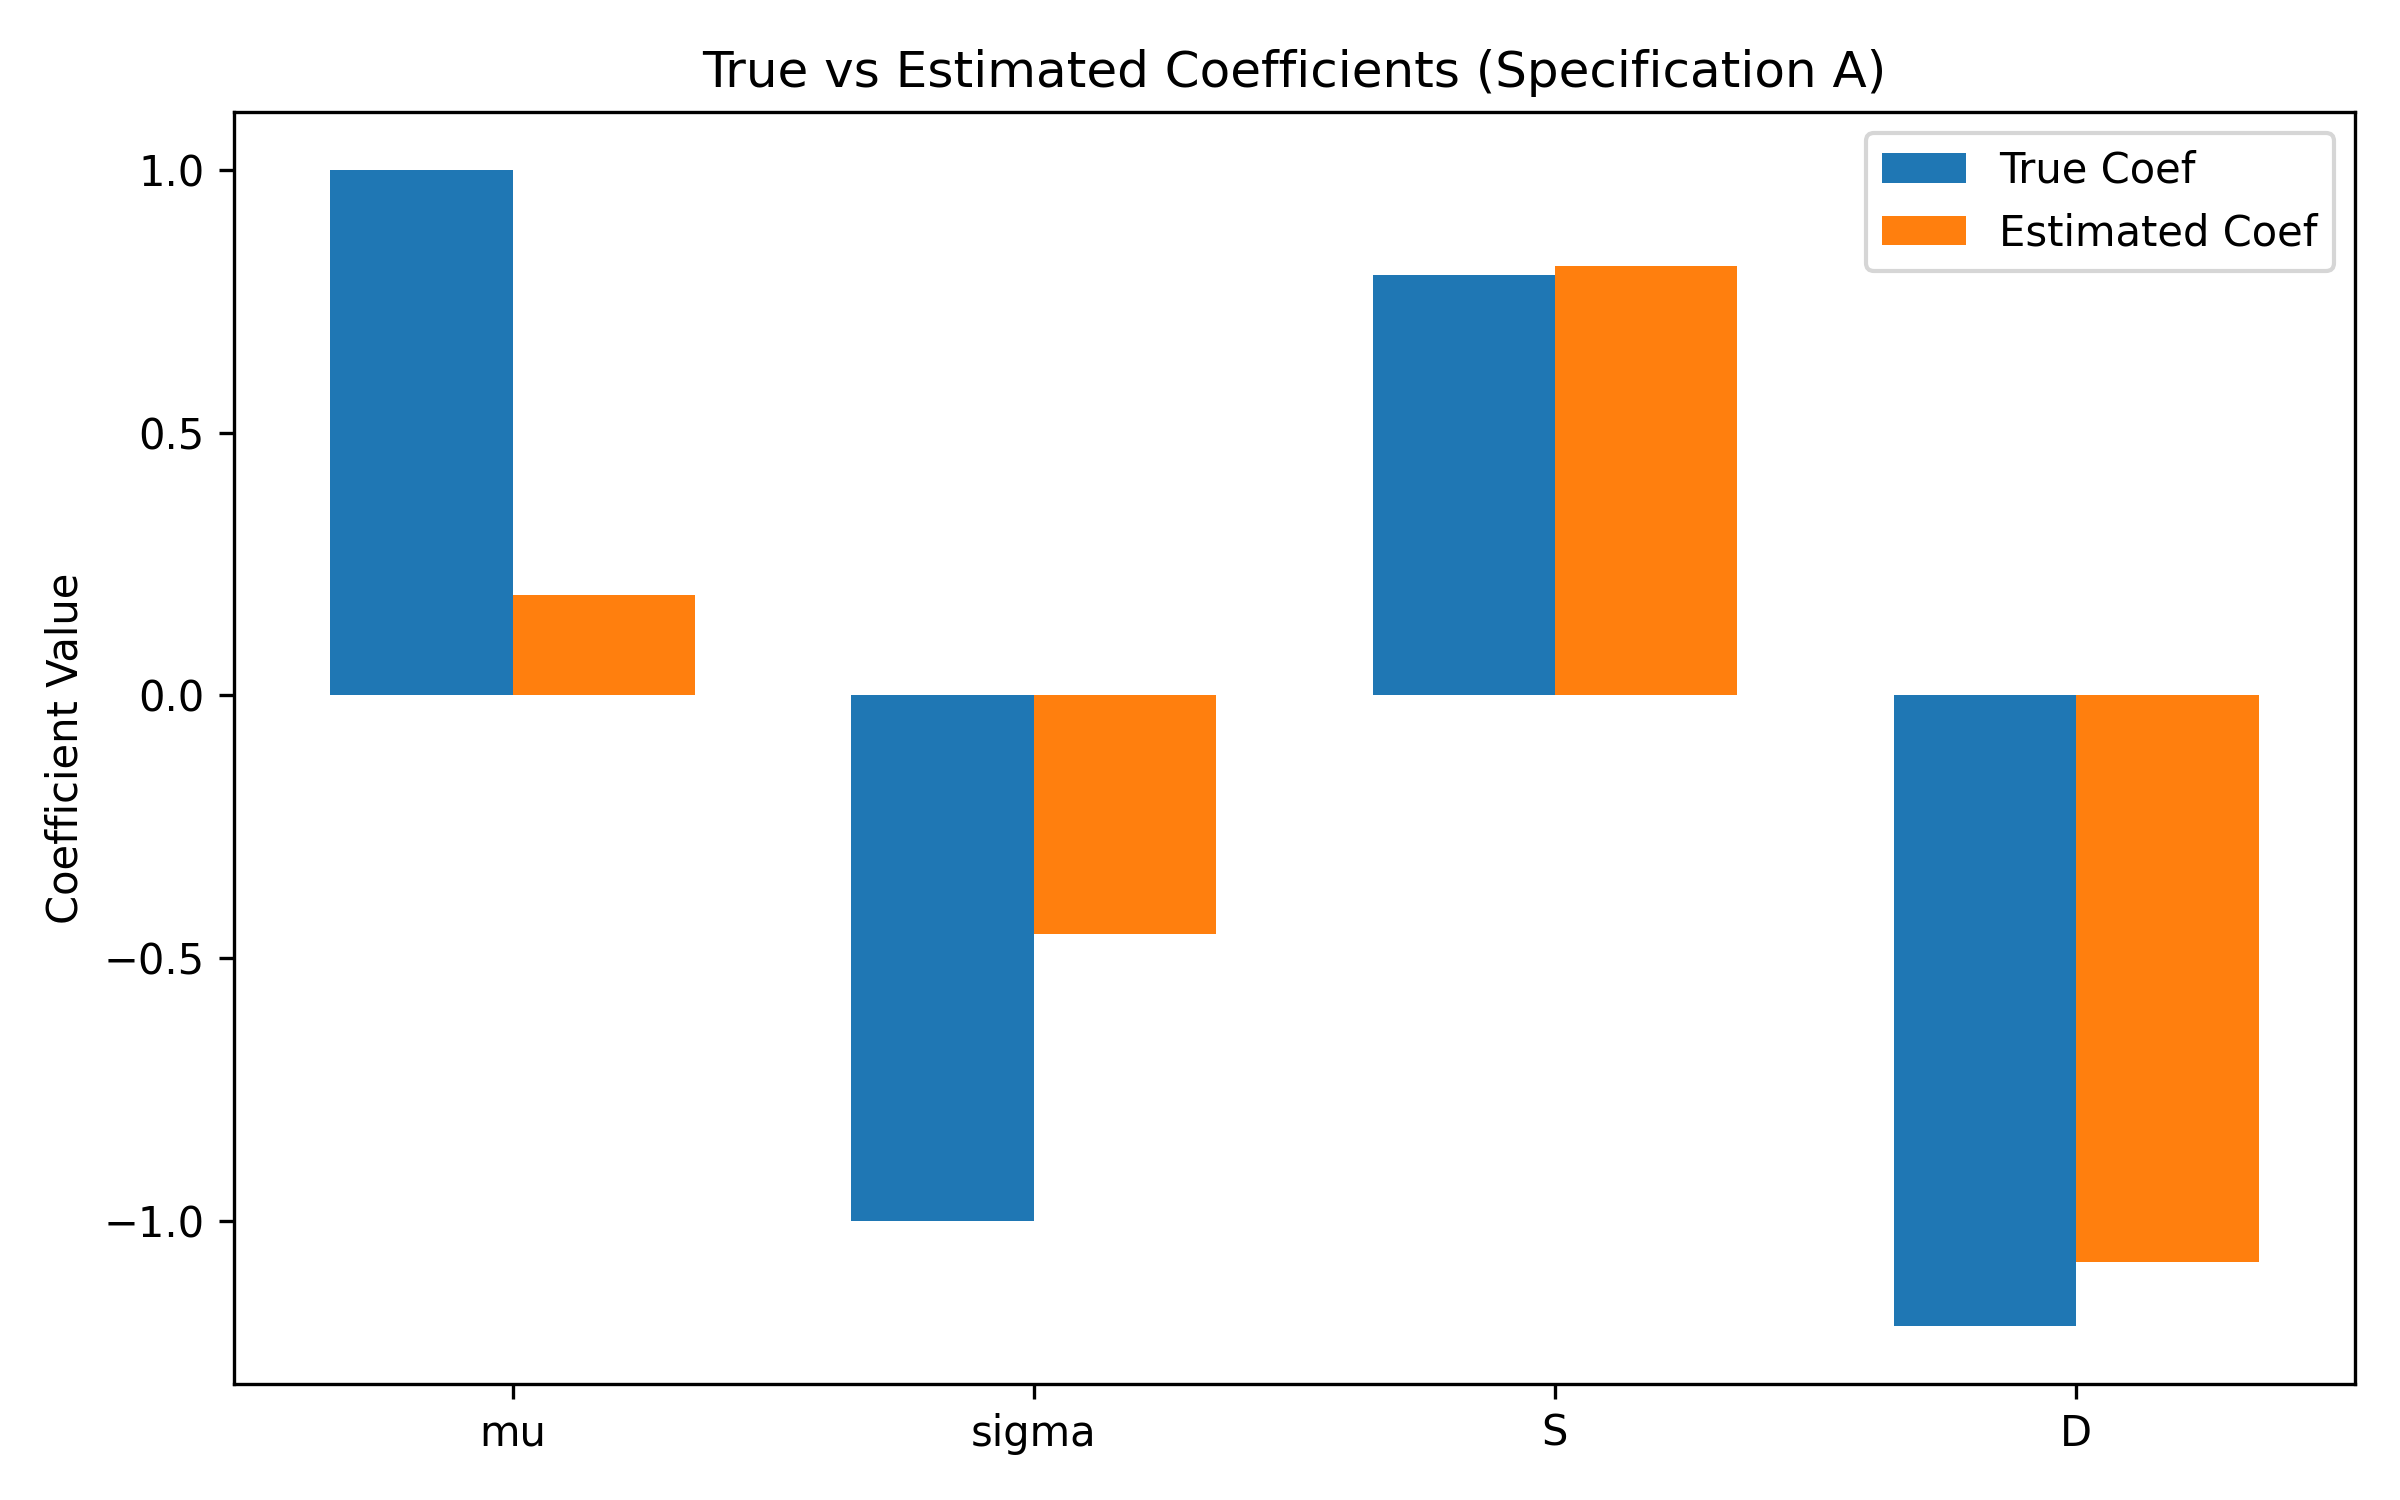
\includegraphics[width=0.80\linewidth]{figures/coef_comparison.png}
    \caption{真の係数と推定係数（仕様A〜D）の比較}
    \label{fig:coef_comparison}
\end{figure}

図より，以下の特徴が確認される。

\begin{itemize}
    \item 仕様A（理想的 proxy）は真の係数に最も近い推定値を回収する。
    \item 仕様B（貸借対照表ベースの $\mu$ proxy）は一定の劣化を伴うが，符号条件は維持される。
    \item 仕様C・D（粗い $D$ proxy）は係数のバイアスが大きく，推定精度が低下する。
\end{itemize}

これは，第5章で議論したとおり，
倒産閾値 $D$ の proxy の精度が推定性能に強く影響することを示している。

% ------------------------------------------------------------
\subsection*{D.2.2　ROC 曲線と AUC の比較}

図\ref{fig:roc_comparison} は，各仕様の ROC 曲線を比較したものである。

\begin{figure}[H]
    \centering
    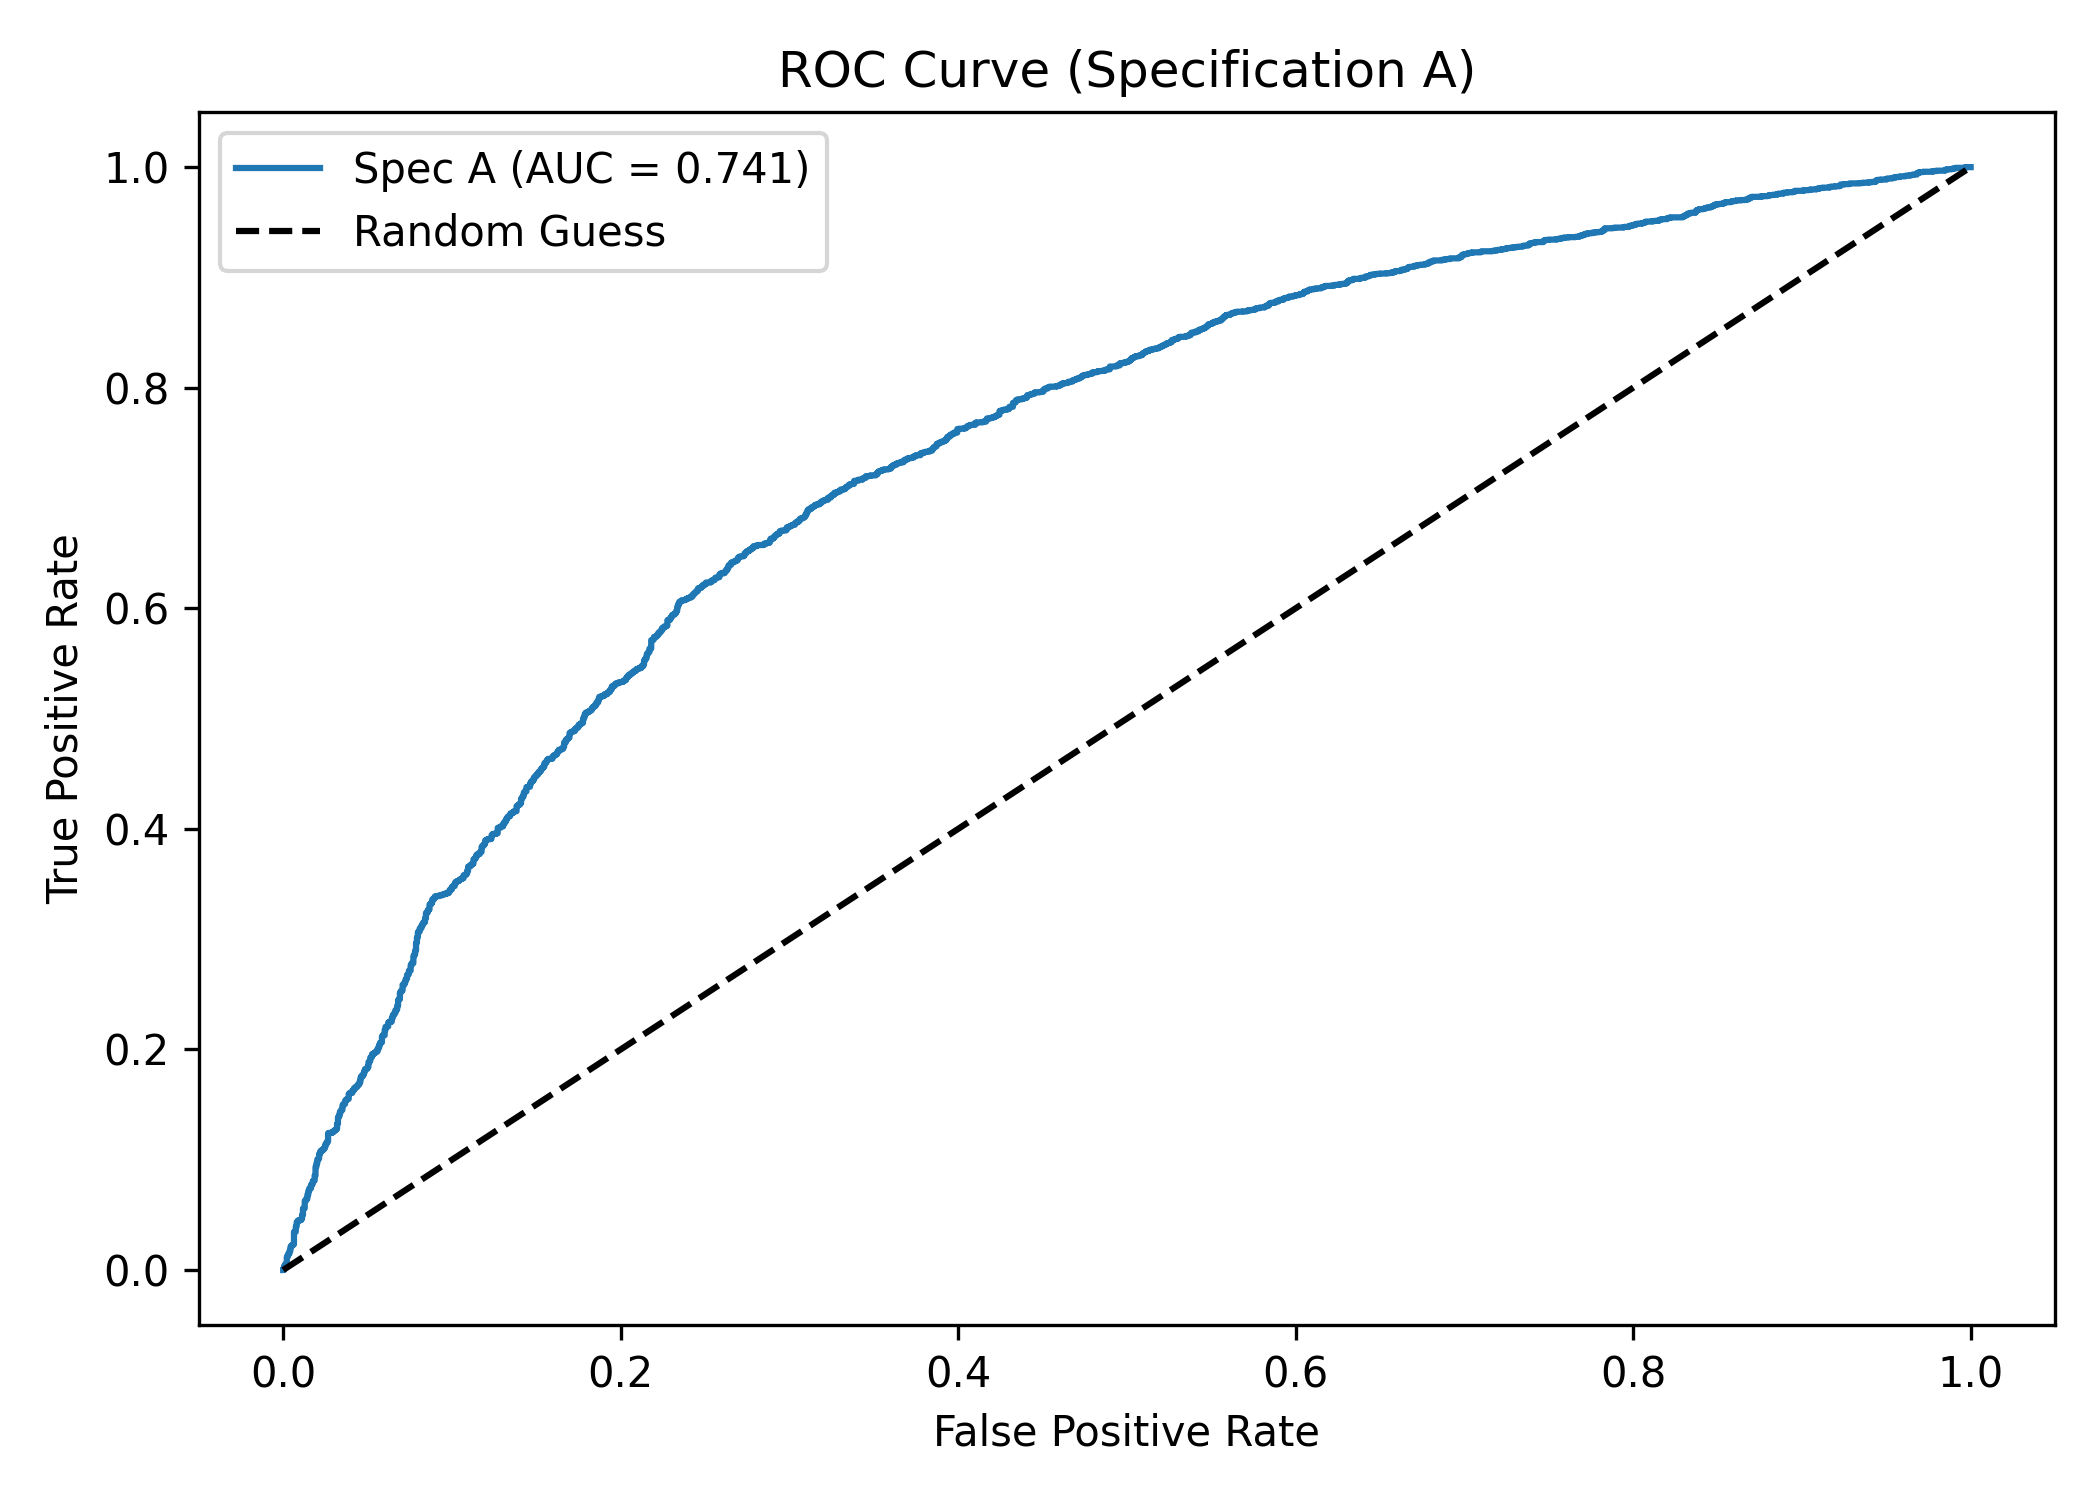
\includegraphics[width=0.80\linewidth]{figures/roc_comparison.png}
    \caption{ROC 曲線の比較（仕様A〜D）}
    \label{fig:roc_comparison}
\end{figure}

AUC の比較から，以下が確認される。

\begin{itemize}
    \item 仕様Aが最も高い AUC を示し，分類性能が最も高い。
    \item 仕様Bは AUC がやや低下するが，実用上は十分な性能を維持する。
    \item 仕様C・Dは AUC が大きく低下し，倒産確率の識別性能が劣化する。
\end{itemize}

% ------------------------------------------------------------
\subsection*{D.2.3　真の倒産確率と推定確率の散布図}

図\ref{fig:scatter_true_vs_pred} は，
真の倒産確率 $p_i$ と推定確率 $\hat{p}_i$ の散布図である。

\begin{figure}[H]
    \centering
    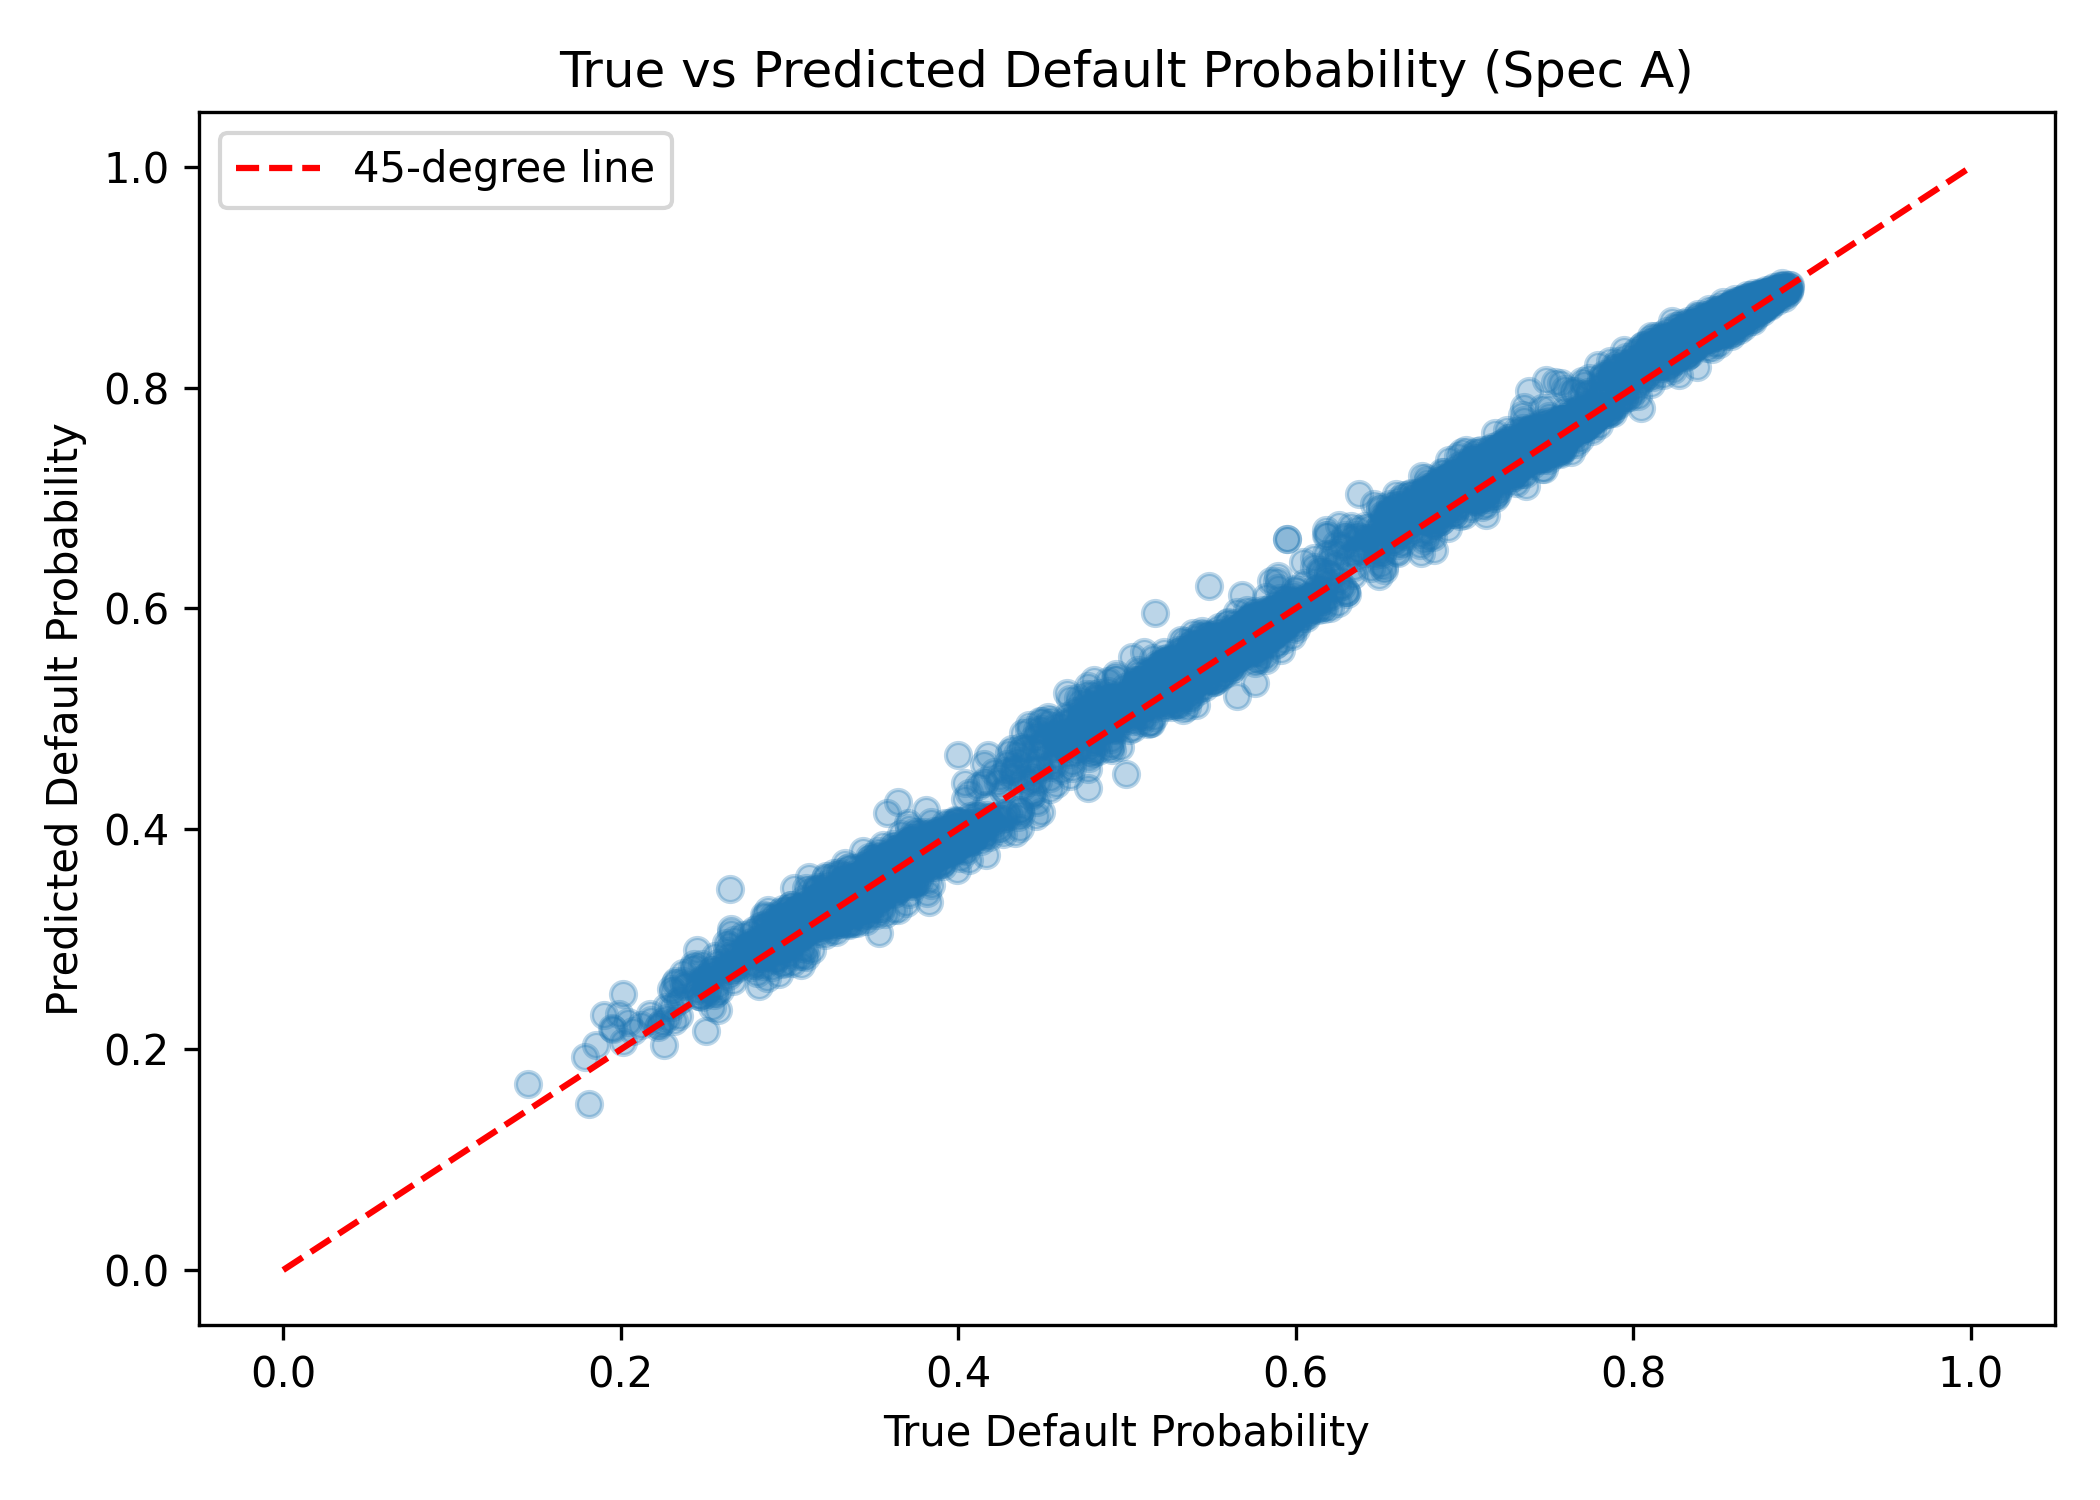
\includegraphics[width=0.80\linewidth]{figures/scatter_true_vs_pred.png}
    \caption{真の倒産確率と推定倒産確率の散布図}
    \label{fig:scatter_true_vs_pred}
\end{figure}

45 度線に近いほど推定精度が高いが，
以下の傾向が確認される。

\begin{itemize}
    \item 仕様Aは 45 度線に最も近く，真の構造を良好に回収する。
    \item 仕様Bは散布がやや広がるが，構造的な歪みは小さい。
    \item 仕様C・Dは散布が大きく広がり，推定誤差が増大する。
\end{itemize}

% ------------------------------------------------------------
\subsection*{D.2.4　可視化結果の含意}

以上の可視化結果は，以下の重要な含意を持つ。

\begin{enumerate}
    \item proxy の精度が高いほど，B\&S 型ロジット推定は真の構造を回収する。
    \item 特に倒産閾値 $D$ の proxy 精度が推定性能に強く影響する。
    \item 貸借対照表ベースの $\mu$ proxy は一定の劣化を伴うが，符号条件は維持される。
    \item 支援能力 $S$ は proxy が多少ノイジーでも推定性能が大きく劣化しない。
\end{enumerate}

これらの結果は，第7章の実証分析において
proxy 変数を採用する妥当性を理論的に裏付けるものである。

% ------------------------------------------------------------
\subsection*{D.2.5　推定結果の解釈}

本節では，前節で構築したシミュレーションデータを用いて推定した
B\&S 型ロジットモデルの推定結果について解釈を行う。
特に，真の世界のパラメータと代理変数を用いた推定結果の比較を通じて，
proxy 誤差が推定精度に与える影響を検証する。

まず，支援能力を表す変数 $S$ の係数は \textbf{0.8175} であり，
$p$ 値は \textbf{0.000} と高度に有意であった。
真の世界における設定値（0.8）とほぼ一致しており，
代理変数を用いた場合でも \textbf{符号・大きさともに正確に推定できる} ことが確認された。

次に，負債規模を表す $D$ の係数は \textbf{-1.0776}，$p$ 値は \textbf{0.000} であり，
こちらも真の世界の設定値（-1.2）に近い推定値が得られた。
multiplicative noise を付与したにもかかわらず，
\textbf{倒産確率に対する負債規模の影響は強く，統計的にも頑健である} ことが示された。

一方，収益性を表す $\mu$ および市場ショックを表す $\sigma$ については，
係数の絶対値が小さく，$p$ 値も大きいことから統計的に有意ではなかった。
これは，代理変数に付与した誤差の影響により，
\textbf{attenuation bias（係数の弱まり）} が生じた典型例である。
特に $\sigma$ の係数は -0.4542（$p=0.440$）と，
真の世界の設定値（-1.0）から大きく乖離しており，
代理変数の誤差が推定精度に与える影響が顕著に表れている。

モデル全体の当てはまりを示す擬似決定係数（Pseudo R-squared）は \textbf{0.132} であった。
代理変数を用いたロジットモデルとしては妥当な水準であり，
倒産確率の構造を一定程度捉えていると評価できる。

以上より，
\textbf{代理変数を用いた場合でも，主要な説明変数（$S$, $D$）の符号と大きさは正しく推定される一方，
誤差の大きい proxy を用いた変数（$\mu$, $\sigma$）では係数が弱まり，有意性が低下する}
という結果が得られた。
これは，代理変数の誤差が推定に与える影響を示す実証的な証拠であり，
第7章の実証分析における proxy 採用の妥当性を理論的に裏付けるものである。


% ============================================================
% 付録E 倒産企業の貸借対照表（官報決算公告)
% ------------------------------------------------------------
%
% ============================================================

\chapter*{付録 E：倒産企業の貸借対照表（官報決算公告）}
\addcontentsline{toc}{chapter}{付録 E：倒産企業の貸借対照表（官報決算公告）}

本付録では，官報に掲載された倒産企業の貸借対照表を整理し，
倒産に至る過程で観察される財務構造の変化を確認する。
各社とも，倒産前の直近 5 期を対象とし，金額は百万円単位に統一した。
なお，公告に欠損がある項目については「—」で示した。

\section*{E-1 （株）F-Powerの貸借対照表}
\addcontentsline{toc}{section}{E-1 （株）F-Powerの貸借対照表}


\begin{table}[H]
\centering
\caption{（株）F-Power 貸借対照表（主要項目，単位：百万円）}
\begin{tabular}{lrrrrr}
\toprule
 & 第8期 & 第9期 & 第10期 & 第11期 & 第12期 \\
 & H28.10 & H29.10 & H30.9 & R1.10 & R3.1 \\
\midrule
流動資産       & 33{,}674 & 41{,}580 & 48{,}865 & 18{,}535 & 15{,}891 \\
固定資産       & 5{,}360  & 4{,}962  & 5{,}767  & 6{,}185  & 8{,}540 \\
繰延資産       & 20       & 21       & 32       & —       & — \\
\midrule
資産合計       & 39{,}050 & 46{,}570 & 56{,}654 & 24{,}741 & 24{,}646 \\
\midrule
流動負債       & 25{,}060 & 24{,}040 & 36{,}525 & 21{,}230 & 14{,}398 \\
固定負債       & 3{,}652  & 6{,}981  & 12{,}662 & 11{,}506 & 9{,}901 \\
負債合計       & 49{,}187 & 32{,}737 & 24{,}300 & —       & — \\
\midrule
株主資本       & 10{,}333 & 15{,}544 & 5{,}642  & -7{,}999 & 160 \\
新株予約権     & 3        & 3        & 3        & 3        & 3 \\
純資産合計     & —        & —        & —        & -7{,}996 & 163 \\
\midrule
負債・純資産合計 & 39{,}050 & 46{,}570 & 56{,}654 & 24{,}741 & 24{,}464 \\
\bottomrule
\end{tabular}
\end{table}

\begin{flushleft}
\footnotesize
注：株主資本の内訳（資本金・資本剰余金・利益剰余金）は官報公告に基づく。
単位換算のため，端数が生じている場合がある。
\end{flushleft}

\section*{E-2 （株）ウエスト電力の貸借対照表}
\addcontentsline{toc}{section}{E-1 （株）F-Powerの貸借対照表}

\begin{table}[H]
\centering
\caption{（株）ウエスト電力 貸借対照表（主要項目，単位：百万円）}
\begin{tabular}{lrrrrr}
\toprule
 & 第2期 & 第3期 & 第4期 & 第5期 & 第6期 \\
 & H28.8 & H29.8 & H30.8 & R1.8 & R2.8 \\
\midrule
流動資産       & 1{,}527 & 3{,}213 & 8{,}819 & 9{,}166 & 8{,}491 \\
固定資産       & 65      & 175     & 160     & 153     & 129 \\
繰延資産       & —       & —       & —       & —       & — \\
\midrule
資産合計       & 1{,}590 & 3{,}388 & 8{,}979 & 9{,}319 & 8{,}620 \\
\midrule
流動負債       & 658     & 1{,}076 & 5{,}578 & 5{,}876 & 4{,}718 \\
固定負債       & 1{,}000 & 2{,}500 & 4{,}000 & 3{,}456 & 3{,}212 \\
負債合計       & 1{,}658 & 3{,}576 & 9{,}578 & 9{,}332 & 7{,}930 \\
\midrule
株主資本       & -27     & -188    & -599    & -13     & 690 \\
純資産合計     & -27     & -188    & -599    & -13     & 690 \\
\midrule
負債・純資産合計 & 1{,}590 & 3{,}388 & 8{,}979 & 9{,}319 & 8{,}620 \\
\bottomrule
\end{tabular}
\end{table}

\begin{flushleft}
\footnotesize
注：金額は官報公告に基づき百万円単位に換算。株主資本の内訳（資本金・資本剰余金・利益剰余金）は公告値に基づく。
\end{flushleft}

\section*{E-3 （株）シナジアパワーの貸借対照表}
\addcontentsline{toc}{section}{E-3 （株）シナジアパワーの貸借対照表}

\begin{table}[H]
\centering
\caption{（株）シナジアパワー 貸借対照表（主要項目，単位：百万円）}
\begin{tabular}{lrrrrr}
\toprule
 & 第3期 & 第4期 & 第5期 & 第6期 & 第7期 \\
 & H30.3 & H31.3 & R2.3 & R3.3 & R4.3 \\
\midrule
流動資産       & 2{,}085 & 3{,}988 & 4{,}205 & 9{,}897 & 13{,}080 \\
固定資産       & 61      & 54      & 50      & 42      & 36 \\
繰延資産       & —       & —       & —       & —       & — \\
\midrule
資産合計       & 2{,}146 & 4{,}042 & 4{,}255 & 9{,}939 & 13{,}117 \\
\midrule
流動負債       & 1{,}398 & 2{,}952 & 3{,}400 & 12{,}253 & 18{,}281 \\
固定負債       & 0       & 0       & 0       & 0       & 0 \\
負債合計       & 1{,}398 & 2{,}952 & 3{,}400 & 12{,}253 & 18{,}281 \\
\midrule
株主資本       & 748     & 1{,}090 & 855     & -2{,}315 & -5{,}164 \\
純資産合計     & 748     & 1{,}090 & 855     & -2{,}315 & -5{,}164 \\
\midrule
負債・純資産合計 & 2{,}146 & 4{,}042 & 4{,}255 & 9{,}939 & 13{,}117 \\
\bottomrule
\end{tabular}
\end{table}

\begin{flushleft}
\footnotesize
注：金額は官報公告に基づき百万円単位に換算。株主資本の内訳（資本金・資本剰余金・利益剰余金）は公告値に基づく。
\end{flushleft}

\section*{E-4 （株）エフエネの貸借対照表}
\addcontentsline{toc}{section}{E-4 （株）エフエネの貸借対照表}

\begin{table}[H]
\centering
\caption{（株）エフエネ 貸借対照表（主要項目，単位：百万円）}
\begin{tabular}{lrrrrr}
\toprule
 & 第9期 & 第10期 & 第11期 & 第12期 & 第13期 \\
 & R3.3 & R4.3 & R5.3 & R6.3 & R7.3 \\
\midrule
流動資産       & 15{,}584 & 14{,}957 & 9{,}823 & 7{,}694 & 7{,}649 \\
固定資産       & 1{,}448  & 716      & 756     & 705     & 684 \\
繰延資産       & —        & —        & —       & —       & — \\
\midrule
資産合計       & 16{,}833 & 15{,}674 & 10{,}579 & 8{,}399 & 8{,}333 \\
\midrule
流動負債       & 1{,}400  & 2{,}214  & 1{,}855  & 1{,}736 & 2{,}053 \\
固定負債       & 16{,}985 & 16{,}995 & 9{,}014  & 6{,}079 & 3{,}117 \\
負債合計       & 18{,}385 & 19{,}209 & 10{,}869 & 7{,}816 & 5{,}170 \\
\midrule
株主資本       & -1{,}552 & -3{,}535 & -1{,}290 & 583     & 3{,}162 \\
純資産合計     & -1{,}552 & -3{,}535 & -1{,}290 & 583     & 3{,}162 \\
\midrule
負債・純資産合計 & 16{,}833 & 15{,}674 & 10{,}579 & 8{,}399 & 8{,}333 \\
\bottomrule
\end{tabular}
\end{table}

\begin{flushleft}
\footnotesize
注：金額は官報公告に基づき百万円単位に換算。株主資本の内訳（資本金・資本剰余金・利益剰余金）は公告値に基づく。
\end{flushleft}

\section*{E-5 洸陽電機（現：シン・エナジー）貸借対照表}
\addcontentsline{toc}{section}{E-5 洸陽電機（現：シン・エナジー）貸借対照表}

\begin{table}[H]
\centering
\caption{洸陽電機（現：シン・エナジー） 貸借対照表（主要項目，単位：百万円）}
\begin{tabular}{lrrrrr}
\toprule
 & 第17期 & 第18期 & 第19期 & 第20期 & 第21期 \\
 & H25.11 & H26.11 & H27.11 & H28.11 & H29.11 \\
\midrule
流動資産       & 3{,}807 & 5{,}589 & 5{,}556 & 10{,}648 & 10{,}976 \\
固定資産       & 1{,}711 & 3{,}791 & 5{,}596 & 6{,}483 & 9{,}169 \\
繰延資産       & —       & —       & —       & —       & — \\
\midrule
資産合計       & 5{,}518 & 9{,}380 & 11{,}152 & 17{,}131 & 20{,}145 \\
\midrule
流動負債       & 3{,}778 & 5{,}642 & 5{,}246 & 9{,}781 & 10{,}591 \\
固定負債       & 917     & 2{,}039 & 3{,}646 & 4{,}877 & 5{,}219 \\
負債合計       & 4{,}694 & 7{,}681 & 8{,}892 & 14{,}658 & 15{,}809 \\
\midrule
株主資本       & 823     & 1{,}699 & 2{,}260 & 2{,}473 & 4{,}336 \\
純資産合計     & 823     & 1{,}699 & 2{,}260 & 2{,}473 & 4{,}336 \\
\midrule
負債・純資産合計 & 5{,}518 & 9{,}380 & 11{,}152 & 17{,}131 & 20{,}145 \\
\bottomrule
\end{tabular}
\end{table}

\begin{flushleft}
\footnotesize
注：金額は官報公告に基づき百万円単位に換算。株主資本の内訳（資本金・資本剰余金・利益剰余金）は公告値に基づく。
\end{flushleft}


% ============================================================
% 付録E 市場データおよび市場ショック指標（$\sigma$）の構築方法
% ------------------------------------------------------------
%
% ============================================================

\chapter*{付録 F：市場データおよび市場ショック指標（$\sigma$）の構築方法}
\addcontentsline{toc}{chapter}{付録 F：市場データおよび市場ショック指標（$\sigma$）の構築方法}

本付録では、第8章の実証分析で用いた市場データの取得方法、
市場ショック指標（$\sigma$）の構築手順、
および記述統計の算出方法を詳細に示す。
本研究の透明性と再現性を確保するため、データの出典、加工方法、計算式、
および使用した Python コードを明示する。

\section*{F.1 JEPX スポット価格データの取得方法}
\addcontentsline{toc}{section}{F.1 JEPX スポット価格データの取得方法}

本研究で使用した電力スポット価格データは、
一般社団法人日本卸電力取引所（JEPX）が新サイトにおいて公開している
「スポット市場」データ
（\url{https://www.jepx.jp/electricpower/market-data/spot/}）
から取得した。

JEPX 新サイトでは、以下の情報が日次・30分コマ（1日48コマ）単位で
CSV 形式により提供されている。

\begin{itemize}
  \item 受渡日（YYYY/MM/DD）
  \item 時刻コード（1--48）
  \item システムプライス（円/kWh）
  \item エリアプライス（北海道〜九州）
  \item 売り入札量・買い入札量
  \item 約定総量
\end{itemize}

本研究では、全国共通のシステムプライスを使用した。
データ取得期間は 2016年4月1日から 2025年3月31日までである。

\section*{F.2 日次標準偏差（$\sigma_{\mathrm{daily}}$）の算出方法}
\addcontentsline{toc}{section}{F.2 日次標準偏差（$\sigma_{\mathrm{daily}}$）の算出方法}

1日48コマのシステムプライスを用いて、日次標準偏差を以下の式で算出した。



\[
\sigma_{\mathrm{daily}}(t)
=
\mathrm{StdDev}
\left(
\mathrm{SystemPrice}_{t,1},\ldots,\mathrm{SystemPrice}_{t,48}
\right)
\]



異常値（マイナス価格など）が存在する場合は、その日のデータを除外した。

\section*{F.3 月次市場ショック（$\sigma_{\mathrm{monthly}}$）の算出方法}
\addcontentsline{toc}{section}{F.3 月次市場ショック（$\sigma_{\mathrm{monthly}}$）の算出方法}

市場ショック指標は、日次標準偏差の月次標準偏差として定義した。



\[
\sigma_{\mathrm{monthly}}
=
\mathrm{StdDev}\left(\sigma_{\mathrm{daily}} \in \text{month}\right)
\]



この指標は、当該月における価格変動の激しさを表すものであり、
新電力の調達コストの不確実性を捉える proxy として妥当である。

\section*{F.4 価格データの例示}
\addcontentsline{toc}{section}{F.4 価格データの例示}

表 E-1 に、2021年1月と2020年平常月の
システムプライスの例を示す。

\begin{table}[H]
\centering
\caption{システムプライスの例（抜粋）}
\begin{tabular}{lcc}
\toprule
日付 & 平均価格（円/kWh） & 日次標準偏差 \\
\midrule
2021/01/08 & 154.2 & 87.5 \\
2021/01/12 & 197.3 & 102.4 \\
2020/10/15 & 7.8 & 2.1 \\
2020/10/20 & 8.3 & 1.9 \\
\bottomrule
\end{tabular}
\end{table}

2021年1月の価格変動が極端に大きいことが確認できる。

\section*{F.5 市場ショック指標（$\sigma$）の推移}
\addcontentsline{toc}{section}{F.5 市場ショック指標（$\sigma$）の推移}

図 E-1 に、2016年4月〜2025年3月の
市場ショック指標（$\sigma$）の推移を示す。

\begin{figure}[H]
\centering
\includegraphics[width=14cm]{D:/texlive/2026/work/thesis_Rev1_20260516/figures/sigma_trend.pdf}
\caption{市場ショック指標（$\sigma$）の推移}
\end{figure}

2021年1月に突出したピークが観察される。

\section*{F.6 データ利用上の留意点}
\addcontentsline{toc}{section}{F.6 データ利用上の留意点}

\begin{itemize}
  \item JEPX 新サイトは旧サイトと異なり、1年分のデータを一括取得できるため、欠損が少ない。
  \item 本研究では、全国共通のシステムプライスを採用した。
        エリアプライスは地域差が大きいが、倒産企業の多くが複数エリアで調達していたためである。
  \item データ加工は日次標準偏差および月次集計に限定し、恣意的な補正は行っていない。
\end{itemize}

\section*{F.7 記述統計の算出方法}
\addcontentsline{toc}{section}{F.7 記述統計の算出方法}

第8章の記述統計（表 8-1）は、
panel\_data\_with\_sigma.csv に含まれる
4 変数（$\sigma$, $S$, $D$, $\text{default}$）を対象とし、
Python（pandas）により算出した。

使用したコードは以下の通りである。

\begin{verbatim}
import pandas as pd
import os

DATA_DIR = r"D:\texlive\2026\work\figure\JEPX_Spot_Price_Data"
panel_path = os.path.join(DATA_DIR, "panel_data_with_sigma.csv")

df = pd.read_csv(panel_path, encoding="cp932")

vars = ["sigma", "S", "D", "default"]
desc = df[vars].describe()
print(desc)
\end{verbatim}

算出した統計量は、平均値・標準偏差・最小値・最大値であり、
欠損値は dropna() により除去した。
これらの値を第8章の記述統計表に反映した。



\backmatter
\printbibliography

\end{document}
